\documentclass[a4paper,12pt]{article} %{article}
\title{Pixton's formula and Abel-Jacobi theory \\on the Picard stack}
%test_edit
%PACKAGES
%%%%%%%%%%%%%%%%%%%%%%%%%%%%%%%%%%%%%%%%%%%%%%%%
\usepackage{amsmath, amssymb, mathrsfs, amsthm, shorttoc, geometry, stmaryrd}% amsfonts, url,, tikz, wrapfig, newclude, }
\usepackage{mathtools} % for \coloneqq (and presumably other stuff!)
\usepackage{hyperref}
\usepackage{xcolor}
\hypersetup{
colorlinks,
linkcolor={black},
citecolor={blue!50!black},
urlcolor={blue!80!black}
}

\newcommand{\MWvone}[1]{}%{#1}
\newcommand{\MWref}[1]{#1}

\newcommand{\mat}[1]{\begin{bmatrix}#1\end{bmatrix}}

\usepackage[all]{xy}
%\usepackage[top=1.5cm, bottom=1.5cm]{geometry}
%\usepackage[left=2cm,right=2cm,top=3cm,bottom=3cm]{geometry}

\usepackage{tabularx}
\usepackage{longtable}
%\numberwithin{equation}{subsection}

%Enumitem
\usepackage{enumitem}
% eg \begin{enumerate}[label={\ref{definition:quasisplit}.\arabic*}]
% eg. \begin{enumerate}[label={1.\arabic*}]

%CLEVEREF STUFF	
\usepackage[capitalise]{cleveref}
%\usepackage{nameref}
\crefformat{equation}{(#2#1#3)}
\let\oref\ref
%\AtBeginDocument{\renewcommand{\ref}[1]{\cref{#1}}}

\usepackage{pgf,tikz}
\usetikzlibrary{matrix, calc, arrows}
%\usetikzlibrary{cd}
\DeclareMathOperator{\coker}{coker}

\usepackage{tikz-cd} %this is the old version, but it also the one the arXiv supports at the moment (2016)

%TODONOTES
%%%%%%%%
%\usepackage{todonotes}
%\setlength{\marginparwidth}{3cm}
%\reversemarginpar

% Double and triple arrows
\makeatletter
\newcommand*{\doublerightarrow}[2]{\mathrel{
  \settowidth{\@tempdima}{$\scriptstyle#1$}
  \settowidth{\@tempdimb}{$\scriptstyle#2$}
  \ifdim\@tempdimb>\@tempdima \@tempdima=\@tempdimb\fi
  \mathop{\vcenter{
    \offinterlineskip\ialign{\hbox to\dimexpr\@tempdima+1em{##}\cr
    \rightarrowfill\cr\noalign{\kern.5ex}
    \rightarrowfill\cr}}}\limits^{\!#1}_{\!#2}}}
\newcommand*{\triplerightarrow}[1]{\mathrel{
  \settowidth{\@tempdima}{$\scriptstyle#1$}
  \mathop{\vcenter{
    \offinterlineskip\ialign{\hbox to\dimexpr\@tempdima+1em{##}\cr
    \rightarrowfill\cr\noalign{\kern.5ex}
    \rightarrowfill\cr\noalign{\kern.5ex}
    \rightarrowfill\cr}}}\limits^{\!#1}}}
\makeatother
%eg
%$A\doublerightarrow{a}{bcdefgh}B$
%$A\triplerightarrow{d_0,d_1,d_2}B$

%MATH OPERATORS
\newcommand{\on}[1]{\operatorname{#1}}
\newcommand{\bb}[1]{{\mathbb{#1}}}
\newcommand{\cl}[1]{{\mathscr{#1}}}
\newcommand{\ca}[1]{{\mathcal{#1}}}
\newcommand{\bd}[1]{{\mathbf{#1}}}

\newcommand{\ul}[1]{{\underline{#1}}}


%Rahul abbreviations:
%%%%%%%%%%%%%%%%%%%%%%%%%%%%%%%%%%%%%%%%%%%%%%%%

\def\D{\mathrm{D}}
\def\d{\mathrm{d}}
\def\tw{\mathrm{tw}}
\def\red{\mathrm{red}}
\def\val{\mathrm{val}}
\def\log{\mathrm{log}}
\def\ev{\mathrm {ev}}
\def\vir{\mathrm {vir}}
\def\ct{\mathrm{ct}}
\def\virt{\mathrm{vir}}
\def\P{\mathsf{P}}
\def\PP{\mathbb{P}}
\def\DR{\mathsf{DR}}
\def\mathsff{{\mathcal{L}}}
\def\CP{{{\mathbb {CP}}}}
\def\oC{\overline{\mathcal{C}}}
\def\ooC{{\mathcal{C}}}
\def\cL{{\mathcal{L}}}
\def\cC{{\mathcal{C}}}
\def\cO{\mathcal{O}}
\def\oM{\overline{\mathcal{M}}}
\def\cM{{\mathcal{M}}}
\def\C{{\mathcal{C}}}
\def\eps{\varepsilon}
\def\Z{\mathbb{Z}}
\def\N{\mathbb{N}}
\def\ZZ{\mathcal{Z}}
\def\ZZZ{\mathsf{Z}}
\def\C{\mathbb{C}}
\def\Q{\mathbb{Q}}
%\def\d{\partial}
\def\qed{{\hfill $\Diamond$}}
\def\cS{{\mathcal S}}
\def\cg{{\mathcal G}}
\def\cR{{\mathcal R}}
\def\Aut{{\rm Aut}}
\def\F{{\mathsf{F}}}
\def\E{\mathrm{E}}
\def\n{\mathrm{n}}
\def\L{\mathrm{L}}
\def\V{\mathrm{V}}
\def\H{\mathrm{H}}
\def\HH{\mathcal{H}}
\def\g{\mathrm{g}}
\def\G{\mathsf{G}}
\def\rarr{\rightarrow}
\def\D{\mathsf{D}}
\def\tP{\widetilde{\mathsf{P}}}
\def\Klog{\omega_{\rm log}}
\def\rmW{\mathsf{W}}
\def\ff{\mathsf{Q}}
\def\fff{\widehat{\mathsf{Q}}}
\def\nice{\displaystyle}
\def\tC{\widetilde{\mathsf{C}}}
\def\ccoarseC{{\mathsf{C}}}
\def\coarseC{\overline{\mathsf{C}}}
\def\coarseL{\mathsf{L}}
\def\tL{\widetilde{{\mathcal L}}}
\def\tS{\widetilde{S}}
\def\tZ{\widetilde{Z}}
\def\oMM{\overline{\mathfrak{M}}}
\def\ooMM{{\mathfrak{M}}}
\def\oCC{\overline{\mathfrak{C}}}
\def\ooCC{{\mathfrak{C}}}
\def\oPP{\overline{\mathfrak{P}}}
\def\Pic{\mathcal{P}ic \,}
\def\ch{{\rm ch}}
\def\td{{\rm td}} 

\def\v{\mathsf{v}}
\def\h{\mathsf{h}}
\def\hH{\mathsf{h}}

%\def\bb{\mathsf{m}}
\def\cc{\ell}

\DeclareMathAlphabet{\mymathbb}{U}{BOONDOX-ds}{m}{n}
\def\zero{\mymathbb{0}}
\def\one{\mymathbb{1}}
\def\A{\mathcal{A}}

%SHEAF VERSIONS OF COMMON OPERATORS
%%%%%%%%%%%%%%%%%%%%%%%%%%%%%%%%%%%%%%%%%%%%%%%%
\def\sheaflie{\mathcal{L}ie}
\def\sheafhom{\mathcal{H}om}

%BRACKETS AND PAIRINGS
%%%%%%%%%%%%%%%%%%%%%%%%%%%%%%%%%%%%%%%%%%%%%%%%
\def\lleft{\left<\!\left<}%{\langle\langle}
\def\rright{\right>\!\right>}%{\rangle\rangle}
\newcommand{\Span}[1]{\left<#1\right>}
\newcommand{\SSpan}[1]{\lleft#1\rright}
\newcommand{\abs}[1]{\lvert#1\rvert}
\newcommand{\aabs}[1]{\lvert\lvert#1\rvert\rvert}

%SUB- AND SUPERSCRIPTS
%%%%%%%%%%%%%%%%%%%%%%%%%%%%%%%%%%%%%%%%%%%%%%%%
\newcommand{\algcl}{^{\textrm{alg}}}
\newcommand{\sepcl}{{^{\textrm{sep}}}}
\newcommand{\urcl}{{^{\textrm{ur}}}}
\newcommand{\ssm}{_{\smooth}}

%FONT ENCODING AND EXOTIC LETTERS
%%%%%%%%%%%%%%%%%%%%%%%%%%%%%%%%%%%%%%%%%%%%%%%%
%\usepackage[OT2,OT1]{fontenc}
%\DeclareSymbolFont{cyrletters}{OT2}{wncyr}{m}{n}
%\DeclareMathSymbol{\Sha}{\mathalpha}{cyrletters}{"58}

\newcommand{\ra}{\rightarrow} %depreciated; use \to
\newcommand{\lra}{\longrightarrow}
\newcommand{\hra}{\hookrightarrow}
\newcommand{\sub}{\subseteq}
\newcommand{\tra}{\rightarrowtail}
\newcommand{\iso}{\stackrel{\sim}{\lra}}


%THEOREMS
%%%%%%%%%%%%%%%%%%%%%%%%%%%%%%%%%%%%%%%%%%%%%%%%
\theoremstyle{definition}
\newtheorem{definition}{Definition} %[section]
\newtheorem{condition}[definition]{Condition}
\newtheorem{problem}[definition]{Problem}
\newtheorem{situation}[definition]{Situation}
\newtheorem{construction}[definition]{Construction}


\newtheorem{remark}[definition]{Remark}
\newtheorem{aside}[definition]{Aside}
\newtheorem{example}[definition]{Example}

\theoremstyle{plain}% default
\newtheorem{conjecture}[definition]{Conjecture}
\newtheorem*{conjectureA}{Conjecture A}
\newtheorem{proposition}[definition]{Proposition}
\newtheorem{lemma}[definition]{Lemma}
\newtheorem{theorem}[definition]{Theorem}
\newtheorem*{theorem*}{Theorem}
\newtheorem{corollary}[definition]{Corollary}
\newtheorem{claim}[definition]{Claim}
\newtheorem{inclaim}{Claim}[definition]

%\theoremstyle{remark}


%MISC
%%%%%%%%%%%%%%%%%%%%%%%%%%%%%%%%%%%%%%%%%%%%%%%%
\def\tam{c_{\tau}} %Tamagawa number
\def\defeq{\stackrel{\text{\tiny def}}{=}}%depreciated: use coloneqq
\newcommand{\linequiv}{\sim_{\text{\tiny lin}}}
\newcommand{\MbarX}{\Mbar_{g,n}(X, \beta)}

%% Some convolutions to redefine \phi as \varphi while storing the original \phi in \phiorig
\usepackage{letltxmacro}
\LetLtxMacro{\phiorig}{\phi}
% \newcommand{\phiorig}{\phi}
\renewcommand{\phi}{\varphi}
\newcommand{\aj}{{\scriptstyle \mathsf{AJ}}}
\newcommand{\vdim}{\mathrm{vdim}}


\newcommand{\cecH}{\check{\on H}}

%\newcounter{temp} 
%\newcommand\interitem[1]{\setcounter{temp}{\value{enumi}}\end{enumerate}{#1}\begin{enumerate}\setcounter{enumi}{\value{temp}}}
%Then use \interitem{text goes here} between two items in a top-level enumerate environment.  It doesn't work inside nested enumerate environments or if you forget to have another item after your interitem text.

\newcommand{\loz}{\lozenge}
\newcommand{\bloz}{\blacklozenge}
\newcommand{\barsigma}{\bar{\sigma}}

\newcommand{\Picabs}{\mathfrak{Pic}}
\newcommand{\Picrel}{\mathfrak{Pic}^{\mathrm{rel}}}
\newcommand{\Chow}{\mathsf{CH}}
\newcommand{\CHop}{\Chow_{\mathsf{op}}}

\newcommand{\tanmap}{\psi}

\newcommand{\invnrI}{I}
\newcommand{\invnrn}{II}
\newcommand{\invnrA}{III}
\newcommand{\invnrII}{IV}
\newcommand{\invnrIII}{V}
\newcommand{\invnrIV}{VI}

% \newcommand{\jocomment}[1]{\textcolor{red}{Jo: #1}}
%\newcommand{\jocomment}[1]{{\color{red}Jo: #1}}
 \newcommand{\jocomment}[1]{}
%\newcommand{\Dcomment}[1]{{\color{blue}D: #1}}
 \newcommand{\Dcomment}[1]{}
%\newcommand{\Rcomment}[1]{{\textbf{\color{red}RP: #1}}}
%\newcommand{\Rosacomment}[1]{{\color{violet}Rosa: #1}}
%\newcommand{\Ycomment}[1]{{\color{brown}Y: #1}}
%AUTHOR DETAILS
%%%%%%%%%%%%%%%%%%%%%%%%%%%%%%%%%%%%%%%%%%%%%%%%
\author{Y. Bae, D. Holmes, R. Pandharipande, J. Schmitt, R. Schwarz}
\date{May 2021}



%COMMENTS
%%%%%%%%%%%%%%%%%%%%%%%%%%%%%%%%%%%%%%%%%%%%%%%%
\newcounter{nootje}
\setcounter{nootje}{1}
\newcommand\todo[1]{[*\thenootje]\marginpar{\tiny\begin{minipage}
{20mm}\begin{flushleft}\thenootje : 
#1\end{flushleft}\end{minipage}}\addtocounter{nootje}{1}}
%\renewcommand{\todo}[1]{}


%Longer versions of proofs
%%%%%%%%%%%%%%%%%%%%%%%%%%%%%%%%%%%%%%%%%%%%%%%%
% \newcommand{\expanded}[1]{#1}
% \renewcommand{\expanded}[1]{}

%SHORTCUTS FOR COMMON COMMANDS
%%%%%%%%%%%%%%%%%%%%%%%%%%%%%%%%%%%%%%%%%%%%%%%%
\newcommand{\beq}{\begin{equation}}%depreciated
\newcommand{\eeq}{\end{equation}}%depreciated
\newcommand{\beqs}{\begin{equation*}}%depreciated
\newcommand{\eeqs}{\end{equation*}}%depreciated

\renewcommand{\k}{k}

\newcommand{\DRop}{\mathsf{DR}^{\mathsf{op}}}

% For using \subset in tikzcd
\tikzset{
  symbol/.style={
    draw=none,
    every to/.append style={
      edge node={node [sloped, allow upside down, auto=false]{$#1$}}}
  }
}
%For rotating labels in tikzcd - added by Rosa 01-04-2020
\tikzset{
    labl/.style={anchor=south, rotate=-90, inner sep=.5mm}
}


\begin{document}
\maketitle
\begin{abstract} 
Let $A=(a_1,\ldots,a_n)$ be a vector of integers with $d=\sum_{i=1}^n a_i$.
By partial resolution of the classical Abel-Jacobi map, we construct a universal
twisted double ramification cycle $\mathsf{DR}^{\mathsf{op}}_{g,A}$ as an operational Chow class
on the Picard stack $\Picabs_{g,n,d}$
of $n$-pointed genus $g$ curves carrying a degree $d$ line bundle. The method of construction
follows the log (and b-Chow) approach to the standard
double ramification cycle with canonical twists on the moduli space of curves \cite{Holmes2017Extending-the-d, Holmes2017Multiplicativit, Marcus2017Logarithmic-com}.



Our main result is a calculation of $\mathsf{DR}^{\mathsf{op}}_{g,A}$ on 
the Picard stack $\Picabs_{g,n,d}$
via an appropriate interpretation of Pixton's formula in the tautological ring. The basic
new tool used in the
proof is the theory of double ramification cycles for target varieties \cite{Janda2018Double-ramifica}.
The formula on the Picard stack is obtained from \cite{Janda2018Double-ramifica} for
target varieties $\mathbb{CP}^n$ in
the limit $n\rightarrow \infty$. The result may be viewed as a
universal calculation in Abel-Jacobi theory.

As a consequence of the calculation of  $\mathsf{DR}^{\mathsf{op}}_{g,A}$ on the Picard stack
$\Picabs_{g,n,d}$, we prove that
the fundamental classes of the moduli spaces of twisted meromorphic differentials
in $\overline{\mathcal{M}}_{g,n}$
are exactly given by Pixton's formula (as conjectured in \cite[Appendix]{Farkas2016The-moduli-spac} and \cite{Schmitt2016Dimension-theor}).
The comparison result  of fundamental classes proven in \cite{Holmes2019Infinitesimal-s} plays a crucial
role in our argument. 
We also prove the set of relations in the
tautological ring of the Picard stack $\Picabs_{g,n,d}$  associated
to Pixton's formula.


\end{abstract}


%\shorttableofcontents{Contents}{1}

\tableofcontents

\newcommand{\Mtildes}{ \widetilde{\ca M}^\Sigma}
\newcommand{\sch}[1]{\textcolor{blue}{#1}}

%new:
\newcommand{\Mbar}{\overline{\ca M}}
\newcommand{\MD}{\ca M^\blacklozenge}
\newcommand{\Md}{\ca M^\lozenge}
\newcommand{\DRL}{\operatorname{DRL}}
%\newcommand{\DR}{\operatorname{DR}}
\newcommand{\DRC}{\operatorname{DRC}}
\newcommand{\isom}{\stackrel{\sim}{\longrightarrow}}
\newcommand{\Ann}[1]{\on{Ann}(#1)}
\newcommand{\fm}{\mathfrak m}
\newcommand{\Mdk}{\Mbar^{\m, 1/\k}}
\newcommand{\field}{K}
\newcommand{\Mdm}{\Mbar^\m}
\newcommand{\m}{{\bd m}}
\newcommand{\cat}[1]{\mathbf{#1}}
%\newcommand{\oM}{\Mbar}
%\newcommand{\cO}{\ca{O}}
%\newcommand{\cM}{\ca{M}}
%\newcommand{\CP}{\bb{P}}
%\newcommand{\C}{\bb{C}}
%\newcommand{\virt}{\mathrm{vir}}
\newcommand{\targetmap}{\ell}
\newcommand{\sourcemap}{\ell'}
\newcommand{\rel}{\mathsf{rel}}
\newcommand{\pre}{\mathsf{pre}}
\setcounter{section}{-1}
\section{Introduction}

\parskip=5pt


\subsection{Double ramification cycles}
\label{Ssec:DRclassic}

Let $A = (a_1, \dots, a_n)$ be a vector of $n$ integers satisfying
%{\footnote{In the twisted case,
%the vanishing sum condition will be removed.}}
$$\sum_{i=1}^n a_i = 0\,. $$ In the moduli space $\cM_{g,n}$ of 
nonsingular curves of genus $g$ with $n$ marked points,
 consider the substack defined by the following classical condition: 
\begin{equation}\label{g445}
\left\{ (C, p_1, \dots, p_n) \in \cM_{g,n} \; \rule[-0.8em]{0.05em}{2em} \; 
\cO_C\Big(\sum_{i=1}^n a_i p_i\Big) \simeq \cO_C \right\}\, . 
\end{equation}
%nd it is natural to ask what is the homology class of its closure or of its natural compactification in $\oM_{g,n}$.
From the point of view of relative Gromov-Witten theory, 
the most natural compactification of the substack \eqref{g445} 
is the space $\oM^{\sim}_{g,A}$ of stable maps to
{\em rubber}\,: stable maps to
 $\CP^1$ relative to $0$ and $\infty$ modulo the $\C^*$-action on $\CP^1$.
The rubber moduli space carries a natural virtual fundamental class $\left[\oM^{\sim}_{g,A}\right]^\virt$ of (complex)
dimension $2g-3+n$. The pushforward 
via the canonical morphism
$$ \epsilon:\oM^{\sim}_{g,A} \rightarrow  \oM_{g,n}$$
is the {\em double ramification cycle} 
$$\epsilon_*\left[\oM^{\sim}_{g,A}\right]^\virt\, =\, \mathsf{DR}_{g,A}\ \in 
{\mathsf{CH}}_{2g-3+n}(\overline{\cM}_{g,n})\,. $$


Double ramification cycles have been studied intensively for the 
past two decades.
Examples of early results can be found in \cite{BSSZ,Cavalieri2011Polynomial-fami,cj,Faber2005Relative-maps-a,Grushevsky2012The-double-rami,Hain2013Normal-function, Marcus2013Stable-maps-to-}.
A complete formula was conjectured by
Pixton in 2014 and proven in \cite{Janda2016Double-ramifica}. 
For subsequent 
study and applications, see \cite{Bae,BGR,CGJZ,FanWu,Farkas2016The-moduli-spac,Holmes2017Extending-the-d,
Holmes2017Jacobian-extens,
Holmes2017Multiplicativit,MPS20,ObPix,Pix18,Schmitt2016Dimension-theor,
Tseng2,Tseng1}. Essential for our work is the formula for double ramification
cycles for target varieties in \cite{Janda2018Double-ramifica}.

We refer the
reader to \cite[Section 0]{Janda2016Double-ramifica} and \cite[Section 5]{RPSLC} for introductions to the subject. For a classical perspective from the point of view
of Abel-Jacobi theory, see 
\cite{Holmes2017Extending-the-d}.



\subsection{Twisted double ramification cycles}
We develop here a theory which extends the study of double ramification
cycles from the moduli space of stable  curves $\overline{\cM}_{g,n}$ to the Picard stack of
curves with line bundles $\Picabs_{g,n}$.
An object of $\Picabs_{g,n}$ over $\mathcal{S}$ is
a flat family $$\pi:\mathcal{C} \rightarrow \mathcal{S}$$ of prestable{\footnote{A prestable $n$-pointed
curve is a connected nodal curve with markings at distinct nonsingular points.
For the entire paper, we avoid the $(g,n)=(1,0)$ case because of 
non-affine stabilizers.}}
    $n$-pointed genus $g$ curves together with a line bundle
    $$\mathcal{L} \rightarrow \mathcal{C}\,. $$
The Picard stack $\Picabs_{g,n}$ is an algebraic (Artin) stack
which is locally of finite type, see \cref{sec:pic_stacks} for a treatment
of foundational issues. 


Since the degree of a line bundle is constant in flat families, there is a
disjoint union
$$\Picabs_{g,n} =\bigcup_{d\in \mathbb{Z}}  \Picabs_{g,n,d}\, ,$$
where $\Picabs_{g,n,d}$ is the Picard stack of curves with degree $d$
line bundles.
Let $$A = (a_1, \dots, a_n)\,,\ \ \ \ \  \sum_{i=1}^n a_i=d \,$$
be a vector of integers.
The first result of the paper is the construction of a 
{\em universal twisted double ramification
cycle} in the operational Chow theory{\footnote{All
Chow theories in the paper will be taken with $\mathbb{Q}$-coefficients.
}} of $\Picabs_{g,n,d}$,
$$\mathsf{DR}^{\mathsf{op}}_{g,A} \in {\mathsf{CH}}^g_{\mathsf{op}}(\Picabs_{g,n,d})\, .$$

The geometric intuition behind the construction is simple.
Let 
$$\pi:\mathcal{C}\rightarrow \mathcal{S}\, ,
\ \ \ \ p_1,\ldots,p_n: \mathcal{S} \rightarrow \mathcal{C}\, ,
\ \ \ \ \mathcal{L}\rightarrow \mathcal{C}$$
be an object of $\Picabs_{g,n,d}$.
The class
$\mathsf{DR}^{\mathsf{op}}_{g,A}$ should operate as the 
locus in the base $\mathcal{S}$ heuristically determined by the condition
$$
\cO_C\Big(\sum_{i=1}^n a_i p_i\Big) \simeq \mathcal{L}|_{C} \,.$$

%To make the above idea precise, we do {\em not} use the virtual class of the moduli space of stable
%maps in Gromov-Witten theory, but rather an alternative approach via log geometry based closely on the stack of %tropical divisors constructed in \cite{Marcus2017Logarithmic-com}. Our construction is presented in Section %\ref{sec:log_def}. We also give a naive interpretation in terms of the closure of the unit section in  $\Picabs$ in the spirit of \cite{Holmes2017Jacobian-extens} (Section \ref{sec:naive_def}), and an interpretation in terms of resolving the indeterminacies of the classical Abel-Jacobi map in the manner of \cite{Holmes2017Extending-the-d} (Section \ref{Sect:AJextension}, where we also describe a b-Chow version in the spirit of \cite{Holmes2017Multiplicativit}). 



To make the above idea precise, we do {\em not} use the virtual class of the moduli space of stable
maps in Gromov-Witten theory, but rather an alternative approach by
partially resolving the classical Abel-Jacobi map.
The method follows the path 
of \cite{Holmes2017Extending-the-d, Holmes2017Multiplicativit}
and
may be viewed  as a universal Abel-Jacobi construction
over the Picard stack. 
Log geometry based on the stack of tropical divisors constructed in \cite{Marcus2017Logarithmic-com}
plays a crucial role.
Our construction is presented in Section \ref{Sect:AJextension}.
%\jocomment{This is close to what we planned to discuss in Section \ref{Sect:AJextension}?}

The basic compatibility of our new operational class $$\mathsf{DR}^{\mathsf{op}}_{g,A} \in {\mathsf{CH}}^g_{\mathsf{op}}(\Picabs_{g,n,d})$$ with the
standard double ramification cycle is as follows.
Let 
$$A = (a_1, \dots, a_n)\,,\ \ \ \ \  \sum_{i=1}^n a_i=0 \,,$$
be given. 
The universal data 
\begin{equation}\label{fftt66677}
\pi: \mathcal{C}_{g,n} \rightarrow \overline{\cM}_{g,n}\, , \ \ \ \ \cO \rightarrow \mathcal{C}_{g,n}
\end{equation}
determine a map $\phi_{\ca O} : \overline{\cM}_{g,n} \to \Picabs_{g,n,0}$.
%Consider the universal family of over the moduli space of
%stable curves
%\begin{equation}\label{fftt55}
%\pi: \mathcal{C}_{g,n} \rightarrow \overline{\cM}_{g,n}
%\end{equation}
%equipped with the trivial line bundle
%\begin{equation}\label{fftt66}
%%\cO_{\mathcal{C}_{g,n}} \rightarrow {\mathcal{C}}_{g,n}\, .
%\end{equation}
%The data \eqref{fftt66677} and \eqref{fftt66} together determine an object of
%$\Picabs_{g,n,0}$.
The action of $\mathsf{DR}^{\mathsf{op}}_{g,A}$ on the fundamental class
of $\overline{\mathcal{M}}_{g,n}$ corresponding to the family \eqref{fftt66677} then equals the previously defined
double ramification cycle
$$\mathsf{DR}^{\mathsf{op}}_{g,A}(\phi_{\ca O})\Big( [\overline{\mathcal{M}}_{g,n}]\Big)= \mathsf{DR}_{g,A}
\in {\mathsf{CH}}_{2g-3+n}(\overline{\mathcal{M}}_{g,n})
\, .$$




More generally, 
for a vector $A = (a_1, \dots, a_n)$ of integers satisfying
$$\sum_{i=1}^n a_i = k(2g-2)\,, $$ 
canonically twisted double ramification cycles,
$$\mathsf{DR}_{g,A, \omega^k}
\in {\mathsf{CH}}_{2g-3+n}(\overline{\mathcal{M}}_{g,n})\, ,$$
related to the classical loci
\begin{equation*}
\left\{ (C, p_1, \dots, p_n) \in \cM_{g,n} \; \rule[-0.8em]{0.05em}{2em} \; 
\cO_C\Big(\sum_{i=1}^n a_i p_i\Big) \simeq  \omega^k_C \right\},\,  
\end{equation*}
have been constructed in
\cite{Guere2016A-generalizatio} for $k=1$ and in \cite{Holmes2017Extending-the-d,Holmes2017Jacobian-extens,Marcus2017Logarithmic-com} for all $k\geq 1$.
The universal data 
\begin{equation}\label{fftt66672}
\pi: \mathcal{C}_{g,n} \rightarrow \overline{\cM}_{g,n}\, , \ \ \ \ \omega_\pi^k \rightarrow \mathcal{C}_{g,n}
\end{equation}
determine a map 
$\phi_{\omega_\pi^k} : \overline{\cM}_{g,n} \to \Picabs_{g,n,k(2g-2)}$. 
Here,
$\omega_\pi$ is the relative dualizing sheaf
of the morphism $\pi$.

The action of $\mathsf{DR}^{\mathsf{op}}_{g,A}$ on the fundamental class
of $\overline{\mathcal{M}}_{g,n}$ corresponding to the family \eqref{fftt66672} is compatible with the constructions of \cite{Guere2016A-generalizatio,Holmes2017Extending-the-d,Holmes2017Jacobian-extens,Marcus2017Logarithmic-com},
$$\mathsf{DR}^{\mathsf{op}}_{g,A} (\phi_{\omega_\pi^k})\Big( [\overline{\mathcal{M}}_{g,n}]\Big)= \mathsf{DR}_{g,A, \omega^k}
\in {\mathsf{CH}}_{2g-3+n}(\overline{\mathcal{M}}_{g,n})
\, $$
for all $k\geq 1$.

The above compatibilities of $\mathsf{DR}^{\mathsf{op}}_{g,A}$ with
the standard and canonically twisted double ramification cycles are proven in Section \ref{proof1111}.

\begin{theorem} \label{cccc}
Let $g\geq 0$ and $d\in \mathbb{Z}$.
Let $A=(a_1,\ldots,a_n)$ be a vector of integers satisfying
$$\sum_{i=1}^n a_i=d\, .$$
Logarithmic compactification of the Abel-Jacobi map yields a universal twisted double
ramification 
cycle
$$\mathsf{DR}^{\mathsf{op}}_{g,A} \in {\mathsf{CH}}^g_{\mathsf{op}}(\Picabs_{g,n,d})$$
which is compatible with the standard double ramification
cycle 
$$\mathsf{DR}_{g,A, \omega^k}\in \mathsf{CH}_{2g-3+n}(\overline{\cM}_{g,n})\, $$
in case $d=k(2g-2)$ for $k\geq 0$.
\end{theorem}

%\{Do we want to mention the targets version here also? I see there is a remark of Johannes here along these %lines commented out, so maybe this has already been discussed? Rahul: no, too much for the intro}

%\jocomment{This seems weaker than the following theorem.}
%\begin{theorem*}
%Let $g\geq 0$, then partial resolution of the Abel-Jacobi map yields a universal twisted double
%ramification 
%cycle
%$$\mathsf{DR}^{\mathsf{op}}_{g} \in {\mathsf{CH}}^g_{\mathsf{op}}(\Picabs_{g,0,0}).$$
%For $A=(a_1, \ldots, a_n) \in \mathbb{Z}^n$ with $\sum_{i=1}^n a_i = k (2g-2)$ the pullback of this cycle by the map
%\[\overline{\cM}_{g,n} \to \Picabs_{g,0,0}, (C,p_1, \ldots, p_n) \mapsto \left(C, \omega_C^{\otimes k} \left( -\sum_{i=1}^n a_i p_i\right) \right),\]
%applied to the fundamental class $[\overline{\cM}_{g,n}]$ gives Holmes' definition of the Double ramification cycle \cite{Holmes2017Extending-the-d}. In particular, for $k=0$ this also recovers the Double ramification cycle defined using the space of rubber relative maps. \jocomment{Similarly, compatibility with DR cycle with targets.}
%\end{theorem*}


\subsection{Pixton's formula}

\subsubsection{Prestable graphs}\label{xvalsg}
We define the set $\G_{g,n}$ of {\em prestable graphs} as
follows. A prestable graph $\Gamma \in \G_{g,n}$ consists of the data
$$\Gamma=(\V\, ,\ \H\, ,\ \L\, , \ \mathrm{g}:\V \rarr \Z_{\geq 0}\, ,
\ v:\H\rarr \V\, , 
\ \iota : \H\rarr \H)$$
satisfying the properties:
\begin{enumerate}
\item[(i)] $\V$ is a vertex set with a genus function $\g:\V\to \Z_{\geq 0}$,
\item[(ii)] $\H$ is a half-edge set equipped with a 
vertex assignment $v:\H \to \V$ and an involution $\iota$,
\item[(iii)] $\E$, the edge set, is defined by the
2-cycles of $\iota$ in $\H$ (self-edges at vertices
are permitted),
\item[(iv)] $\L$, the set of legs, is defined by the fixed points of $\iota$ and is
placed in bijective correspondence with a set of $n$ markings,
\item[(v)] the pair $(\V,\E)$ defines a {\em connected} graph
satisfying the genus condition 
$$\nice \sum_{v \in \V} \g(v) + h^1(\Gamma) = g\, .$$
%\item[(vi)] for each vertex $v$, the stability condition holds: 
%$$2\g(v)-2+ \n(v) >0\, ,$$
%where $\n(v)$ is the valence of $\Gamma$ at $v$ including 
%both edges and legs.
\end{enumerate}
To emphasize $\Gamma$, the notation $\V(\Gamma)$, $\H(\Gamma)$, $\L(\Gamma)$, and $\E(\Gamma)$ will also be used for the vertex, half-edges, legs, and
edges of $\Gamma$. 

An isomorphism between $\Gamma$, $\Gamma' \in \G_{g,n}$ 
consists of bijections $\V \to \V'$ and $\H \to \H'$ respecting the
structures $\L$, $\mathrm{g}$, $v$, and $\iota$.
Let $\Aut(\Gamma)$ denote the automorphism group of $\Gamma$.

% An automorphism of $\Gamma \in \G_{g,n}$ 
% consists of automorphisms
% of the sets $\V$ and $\H$ which leave invariant the
% structures $\L$, $\mathrm{g}$, $v$, and $\iota$.
% Let $\Aut(\Gamma)$ denote the automorphism group of $\Gamma$.


While the set of isomorphism classes of prestable graphs is infinite, the set of isomorphism classes of prestable graphs with prescribed bounds on the number of edges is finite.
% subsets consisting of
% prestable graphs with prescribed bounds on the number of edges contain only finitely many isomorphism classes. 



Let $\mathfrak{M}_{g,n}$ be the algebraic (Artin) stack of prestable curves of genus $g$ with $n$ marked points.
A prestable graph $\Gamma$ determines an algebraic stack $\mathfrak{M}_\Gamma$ of 
curves
with degenerations forced by the graph,
$$
\mathfrak{M}_\Gamma = \prod_{v \in \V} \mathfrak{M}_{\g(v), \n(v)}\, $$
together with a 
canonical\footnote{To define the map, we choose an ordering on the half-edges at each vertex. } map
$$j_\Gamma : \mathfrak{M}_\Gamma \to \mathfrak{M}_{g,n}\, .$$
Since $\mathfrak{M}_{g,n}$ is smooth and
the morphism $j_\Gamma$ is proper, representable, and lci, we obtain an operational Chow class on the algebraic
stack of curves,
$$j_{\Gamma*}[\mathfrak{M}_\Gamma] \in \mathsf{CH}_{\mathsf{op}}^{|\E(\Gamma)|}(\mathfrak{M}_{g,n})\, .$$
Via the morphism of algebraic stacks,
$$\epsilon: \Picabs_{g,n,d} \rightarrow \mathfrak{M}_{g,n}\, ,$$
$j_{\Gamma*}[\mathfrak{M}_\Gamma]$ also defines an operational Chow class
on the Picard stack,
$$\epsilon^* j_{\Gamma*}[\mathfrak{M}_\Gamma] \in \mathsf{CH}_{\mathsf{op}}^{|\E(\Gamma)|}(\Picabs_{g,n,d})\, .$$

\subsubsection{Prestable graphs with degrees} \label{Sect:Prestgrwdeg}
We will require a refinement of the prestable graphs of Section \ref{xvalsg} which includes degrees
of line bundles. 

We define the set $\G_{g,n,d}$ of {\em prestable graphs of degree $d$} as
follows: $$\Gamma_\delta=(\Gamma,\delta) \in \G_{g,n,d}$$ consists of the data
\begin{enumerate}
    \item[$\bullet$] a prestable graph $\Gamma\in \mathsf{G}_{g,n}$,
    \item[$\bullet$] a function $\delta: \V \rightarrow \mathbb{Z}$
    satisfying the degree condition
$$\sum_{v\in V} \delta(v) = d\, .$$
\end{enumerate}
The function $\delta$ is  often called the {\em multidegree}.


An automorphism of $\Gamma_\delta \in \G_{g,n,d}$ 
consists of an automorphism of $\Gamma$
leaving $\delta$ invariant.
Let $\Aut(\Gamma_\delta)$ denote the automorphism group of $\Gamma_\delta$.


%For a prestable graph $\Gamma\in \mathsf{G}_{g,n}$ and a function $\delta:V \rightarrow \mathbb{Z}$
%which satisfies the degree condition (vi), let $\Gamma_\delta\in \mathsf{G}_{g,n,d}$ be the associated
%prestable graph of degree $d$.

For $\Gamma_\delta\in \mathsf{G}_{g,n,k}$, let $\mathfrak{M}_\Gamma$ be the algebraic stack of
curves defined in Section \ref{xvalsg} with respect to the underlying prestable graph $\Gamma$. 
Let
$\Picabs_{\Gamma_\delta}$ be the Picard stack,
$$\epsilon:\Picabs_{\Gamma_\delta} \rightarrow \mathfrak{M}_{\Gamma}\, ,$$
parameterizing curves with degenerations forced by $\Gamma$ and with  line bundles which
have 
degree $\delta(v)$ restriction to the components corresponding to the vertex $v\in \V$.
We have a
canonical map
$$j_{\Gamma_\delta} : \Picabs_{\Gamma_\delta} \to \Picabs_{g,n,d}\, .$$
Since $\Picabs_{g,n,d}$ is smooth and
the morphism $j_{\Gamma_\delta}$ is proper, representable, and lci,
we obtain an operational Chow class,
$$j_{\Gamma_\delta *}[\Picabs_{\Gamma_\delta}] \in \mathsf{CH}_{\mathsf{op}}^{|\E(\Gamma)|}(\Picabs_{g,n,d})\, .$$
As operational Chow classes, the following formula holds:
\begin{equation}\label{5599w}
\epsilon^*j_{\Gamma*}[\mathfrak{M}_\Gamma] = \sum_{\delta} j_{\Gamma_\delta *}[\Picabs_{\Gamma_\delta}]
\ \in \mathsf{CH}_{\mathsf{op}}^{|\E(\Gamma)|}(\Picabs_{g,n,d})
\, ,
\end{equation}
where the sum{\footnote{The sum is infinite, but only finitely many terms
are nonzero in any operation.}} is over all functions $\delta:\V \rightarrow \mathbb{Z}$ satisfying the degree condition.
Equivalently, we may write \eqref{5599w} as
\begin{equation*}
\frac{1}{|{\text{Aut}}(\Gamma)|}\, \epsilon^*j_{\Gamma*}[\mathfrak{M}_\Gamma] = 
\sum_{\Gamma_\delta\in \mathsf{G}_{g,n,d}} 
\frac{1}{|{\text{Aut}}(\Gamma_\delta)|}\, 
j_{\Gamma_\delta *}[\Picabs_{\Gamma_\delta}]\ 
\in \mathsf{CH}_{\mathsf{op}}^{|\E(\Gamma)|}(\Picabs_{g,n,d})
\, ,
\end{equation*}
where the sum on the right side is now over all isomorphism classes of
prestable graphs of degree $d$ with underlying prestable graph $\Gamma$.

\subsubsection{Tautological \texorpdfstring{$\psi$}{psi}, \texorpdfstring{$\xi$}{xi}, and \texorpdfstring{$\eta$}{eta} classes} \label{Ssec:PsiXiEta}

The universal curve $$\pi:\mathfrak{C}_{g,n} \to \Picabs_{g,n}$$ 
carries two natural line bundles: the relative dualizing sheaf $\omega_{\pi}$ 
and the universal line bundle
$$\mathfrak{L} \rightarrow \mathfrak{C}_{g,n}\, .$$
Let $p_i$ be the $i$th section of the universal curve, let 
$$\mathfrak{S}_i\subset \mathfrak{C}_{g,n}$$
be  the corresponding divisor, and let
$$\omega_\log = \omega_\pi\Big(\sum_{i=1}^n \mathfrak{S}_i\Big)$$ be the relative log-canonical line bundle 
with first Chern class $c_1 (\omega_\log)$. 
Let $$\xi = c_1(\mathfrak{L})$$ be the first Chern class of $\mathfrak{L}$.

\begin{definition} \label{Not:PsiXiEta}
The following operational classes on $\Picabs_{g,n}$ are obtained from the
universal structures:
\begin{itemize}
    \item $\psi_i = c_1(p_i^* \omega_\pi)\in \mathsf{CH}^1_{\mathsf{op}}(\Picabs_{g,n})\, $,
    \item $\xi_i = c_1(p_i^* \mathfrak{L})\in \mathsf{CH}^1_{\mathsf{op}}(\Picabs_{g,n})
    \, $,
    \item $\eta_{a,b} = \pi_*\left(c_1(\omega_\log)^a \xi^b\right)
    \in \mathsf{CH}^{a+b-1}_{\mathsf{op}}(\Picabs_{g,n})
    \, $.
\end{itemize}
\end{definition}
For simplicity in the formulas, 
we will use the
notation
$$\eta= \eta_{0,2} =\pi_*(\xi^2)\, .$$
The standard $\kappa$ classes are defined by the $\pi$ pushforwards
of powers of $c_1(\omega_\log)$, 
$$\eta_{a,0} = \kappa_{a-1}\, .$$

\begin{definition}
A {\em decorated prestable graph} $[\Gamma_\delta,\gamma]$ {\em of degree $d$} 
%of type $(g,n,\beta)$ 
is a prestable graph $\Gamma_\delta \in \G_{g,n,d}$ of degree $d$ together with the following
decoration data $\gamma$:
\begin{itemize}
\item each leg $i\in \L$ is decorated with a monomial $\psi_i^a \xi_i^b$,
\item each half-edge $h\in \H\setminus \L$ is 
decorated with a monomial $\psi^a_h$,
\item each edge $e\in \E$ is decorated with a monomial $\xi^a_e$,
\item each vertex in $\V$ is decorated with a monomial in the variables 
$\{\eta_{a,b}\}_{a+b \geq 2}$.
\end{itemize}
In all four cases, the monomial may be be trivial.
\end{definition}


Let $\D\G_{g,n,d}$ be the set of decorated prestable graphs of degree $d$.
To each decorated graph of degree $d$, 
$$[\Gamma_\delta,\gamma]\in \D\G_{g,n,d}\,,$$ we assign the 
operational class 
$$j_{\Gamma_\delta*}[\gamma] \in \mathsf{CH}^*_{\mathsf{op}}(\Picabs_{g,n,d})$$
obtained
via the proper representable morphism
$$j_{\Gamma_\delta} : \Picabs_{\Gamma_\delta} \rightarrow \Picabs_{g,n,d}$$
and the action of the decorations.

The action of decorations is described
as follows.
Given $\Gamma_\delta\in \mathsf{G}_{g,n,k}$, the stack $\Picabs_{\Gamma_\delta}$ admits a morphism{\footnote{The fibers of the map are torsors under the group $\mathbb{G}_m^{h^1(\Gamma)}$.}}
\[\Picabs_{\Gamma_\delta} \to \prod_{v \in \V(\Gamma_\delta)} \Picabs_{\g(v),\n(v),\delta(v)}\]
which sends a line bundle $\mathcal{L}$ on a prestable curve $\mathcal{C}$ to its restrictions on the various components,
$$ \mathcal{L}|_{\mathcal{C}_v}\, , \  \ \  v\in \V(\Gamma_\delta)\, . $$
For $v \in \V(\Gamma_\delta)$, we define the operational
class $\eta(v)$ on $\Picabs_{\Gamma_\delta}$ as the pullback of the operational class $\eta$ on the factor $\Picabs_{\g(v),\n(v),\delta(v)}$ above. The operational
classes $\psi$ at the markings and $\xi$ at the half-edges are
defined similarly.




\begin{definition} The {\em tautological  classes} in
 $\mathsf{CH}^*_{\mathsf{op}}(\Picabs_{g,n,d})$ consist of the 
 $\mathbb{Q}$-linear span
 of the operational classes associated to 
 all $[\Gamma_\delta,\gamma]\in \D\G_{g,n,d}$.
\end{definition}

By standard analysis \cite{GraberPandharipande}, the tautological classes
have a natural ring structure.
Our formula for $\mathsf{DR}_{g,A}^{\mathsf{op}}$ 
will be a sum of operational classes
determined by decorated prestable graphs of degree $d=\sum_{i=1}^n a_i$
(and hence will be tautological).

\subsubsection{Weightings mod \texorpdfstring{$r$}{r}} \label{Ssec:weightings}
Let $\Gamma_\delta\in \G_{g,n,d}$ be a prestable graph of degree $d$, and
let $r$ be a positive integer.

\begin{definition} A {\em weighting mod~$r$} of $\Gamma_\delta$ is a function on the set of half-edges,
$$ w:\H(\Gamma_\delta) \rightarrow \{0,1, \ldots, r-1\}\, ,$$
which satisfies the following three properties:

\begin{enumerate}
\item[(i)] $\forall i\in \L(\Gamma_\delta)$, corresponding to
 the marking $i\in \{1,\ldots, n\}$,
$$w(i)=a_i  \mod r\, ,$$
\item[(ii)] $\forall e \in \E(\Gamma_\delta)$, corresponding to two half-edges
$h,h' \in \H(\Gamma_\delta)$,
$$w(h)+w(h')=0 \mod r\, ,$$
\item[(iii)] $\forall v\in \V(\Gamma_\delta)$,
$$\sum_{v(h)= v} w(h)= \delta(v) \mod r\, ,$$ 
where the sum is taken over {\em all} $\mathsf{n}(v)$ half-edges incident 
to $v$.\end{enumerate}
\end{definition}



We denote by $\mathsf{W}_{\Gamma_\delta,r}$ the finite set of all possible weightings
mod $r$
of
$\Gamma_\delta$. The set $\mathsf{W}_{\Gamma_\delta,r}$ has cardinality $r^{h^1(\Gamma_\delta)}$.
We view $r$ as a {\em regularization parameter}.

\subsubsection{Calculation of the twisted double ramification cycle} \label{Ssec:MainFormula}
We denote by
$\P_{g,A,d}^{c,r}\in \mathsf{CH}^c_{\mathsf{op}}(\Picabs_{g,n,d})$
the codimension{\footnote{Codimension here is usually
called degree. But since we already have line bundle degrees,
we use the term codimension for clarity.}}
 $c$ component of the tautological operational class 
\begin{multline*}
\hspace{-10pt}\sum_{
\substack{\Gamma_\delta\in \G_{g,n,d} \\
w\in \mathsf{W}_{\Gamma_\delta,r}}
}
\frac{r^{-h^1(\Gamma_\delta)}}{|\Aut(\Gamma_\delta)| }
\;
j_{\Gamma_\delta*}\Bigg[
\prod_{i=1}^n \exp\left(\frac12 a_i^2 \psi_i + a_i \xi_i \right)
\prod_{v \in \V(\Gamma_\delta)} \exp\left(-\frac12 \eta(v) \right)
\\ \hspace{+10pt}
\prod_{e=(h,h')\in \E(\Gamma_\delta)}
\frac{1-\exp\left(-\frac{w(h)w(h')}2(\psi_h+\psi_{h'})\right)}{\psi_h + \psi_{h'}} \Bigg]\, .
\end{multline*} 
Several remarks about the formula are required:
\begin{enumerate}
    \item[(i)]
    The sum is over all isomorphism classes of prestable graphs of degree $d$ in the
    set $\mathsf{G}_{g,n,d}$. 
    Only finitely many underlying prestable graphs $\Gamma\in \mathsf{G}_{g,n}$ can
    contribute in fixed codimension $c$. However, for each such prestable graph, the above formula
    has infinitely many summands corresponding to the infinitely many functions
    $$\delta: \V \rightarrow \mathbb{Z}$$
    which satisfy the degree condition.
    The operational Chow class $\P_{g,A,d}^{c,r}$ is nevertheless well-defined since
      only finitely many summands have nonvanishing operation on any given family of curves
       carrying a degree $d$ line bundle over a base $\mathcal{S}$ of finite type.
    \item[(ii)] 
    Once the prestable graph $\Gamma_\delta$ is chosen, we sum over all $r^{h^1(\Gamma_\delta)}$ different 
    weightings $w\in \mathsf{W}_{\Gamma_\delta,r}$.
    \item[(iii)]
Inside the pushforward in the above formula, the first product 
$$\prod_{i=1}^n \exp\left(\frac{1}{2}a_i^2 \psi_{h_i}+a_i \xi_{h_i}\right)\, $$
is over $h\in \L(\Gamma)$
via the correspondence of legs and markings.
\item[(iv)]The class $\eta(v)$ is the $\eta_{0,2}$ class 
of Definition \ref{Not:PsiXiEta} associated to the vertex.
\item[(v)]
The third product is over all $e\in \E(\Gamma_\delta)$.
The factor 
$$\frac{1-\exp\left(-\frac{w(h)w(h')}{2}(\psi_h+\psi_{h'})\right)}{\psi_h + \psi_{h'}}$$
is well-defined since 
\begin{enumerate}
\item[$\bullet$]
the denominator formally divides
the numerator,
\item[$\bullet$] the factor is symmetric in $h$ and $h'$.
\end{enumerate}
No edge orientation is necessary.
\end{enumerate}

The following fundamental polynomiality property of $\P_{g,A,d}^{c,r}$ 
 is
parallel to Pixton's polynomiality in \cite[Appendix]{Janda2016Double-ramifica} and
is a consequence of \cite[Proposition $3''$]{Janda2016Double-ramifica}.

\begin{proposition} \label{pply} For fixed $g$, $A$, $d$, and $c$ and a decorated graph $[\Gamma_\delta, \gamma]$ of
degree $d$, the coefficient of $j_{\Gamma_\delta*} [\gamma]$ in the
tautological class
$$\P_{g,A,d}^{c,r} \in \mathsf{CH}^c_{\mathsf{op}}(\Picabs_{g,n,d})$$
is polynomial in $r$ (for all sufficiently large $r$).
\end{proposition}

We denote by $\P_{g,A,d}^c$ the value at $r=0$ 
of the polynomial associated to $\P_{g,A,d}^{c,r}$ by Proposition~\ref{pply}. In other words, $\P_{g,A,d}^c$ is the {\em constant} term of the associated polynomial in $r$. 

The main result of the paper is a 
 formula for the universal twisted double ramification cycle in operational Chow.{\footnote{Our
handling of the prefactor $2^{-g}$ in \cite[Theorem 1]{Janda2016Double-ramifica} differs here.
The factors of $2$ are now placed in the definition of $\P_{g,A,d}^{c,r}$
as in \cite{Janda2018Double-ramifica}}


\begin{theorem} \label{Thm:main}
Let $g\geq 0$ and $d\in \mathbb{Z}$.
Let $A=(a_1,\ldots,a_n)$ be a vector of integers with
$\sum_{i=1}^n a_i=d\,$.
The universal twisted double ramification cycle is calculated by Pixton's formula:
$$\mathsf{DR}^{\mathsf{op}}_{g,A} =\P_{g,A,d}^g\
\in {\mathsf{CH}}^g_{\mathsf{op}}(\Picabs_{g,n,d})\, .$$
\end{theorem}



Theorem \ref{Thm:main} is the most fundamental formulation of the relationship
between Abel-Jacobi theory and Pixton's formula that we know. Certainly,  
Theorem \ref{Thm:main} 
implies the double ramification cycle and $X$-valued
double ramification cycle results of \cite{Janda2016Double-ramifica,Janda2018Double-ramifica} }. But since we will
use \cite{Janda2018Double-ramifica} in the proof of Theorem \ref{Thm:main}, we provide no new approach to
these older results. However, the additional depth of Theorem \ref{Thm:main} immediately
allows new applications.


\subsection{Vanishing}
From his original double
ramification cycle formula,
Pixton conjectured an associated
vanishing property in the
tautological ring of the moduli
space of curves which
was proven by Clader and Janda \cite{cj}.
The parallel vanishing statement
in the tautological ring of the
moduli space of stable maps to $X$
was proven in \cite{Bae}.
The most general vanishing
statement is the following
result.


\begin{theorem} \label{Thm:mainvan}
Let $g\geq 0$ and $d\in \mathbb{Z}$.
Let $A=(a_1,\ldots,a_n)$ be a vector of integers with
$\sum_{i=1}^n a_i=d$.
 Pixton's vanishing holds
 in operational Chow:
$$ \P_{g,A,d}^c\ = 0 \
\in {\mathsf{CH}}^c_{\mathsf{op}}(\Picabs_{g,n,d})\, \ \ \ 
{\text{for all}} \ \ c>g\, .
$$ 
\end{theorem}

 



Theorem \ref{Thm:mainvan} may be viewed
as providing relations among
tautological classes in the operational
Chow ring of the Picard stack -- a new
direction of study with many open questions.{\footnote{See \cite{RandalWilliams2012,Yin}
for tautological relations on the Picard variety over
the moduli space of smooth curves.}}
While Theorem \ref{Thm:mainvan} 
implies the
vanishings of
\cite{Bae, cj}, 
we will use these results in our
proof. 


\subsection{Twisted holomorphic and meromorphic differentials} \label{Sect:Twistdiffintro}
\subsubsection{Fundamental classes}
Let $A=(a_1,\ldots,a_n)$ be a vector of zero and pole multiplicities
satisfying
$$\sum_{i=1}^n a_i= 2g-2\, .$$
Let $\HH_g(A) \subset \mathcal{M}_{g,n}$ be the quasi-projective locus 
of pointed curves $(C,p_1,\ldots,p_n)$ satisfying the condition
$$\mathcal{O}_C\Big(\sum_{i=1}^n a_i p_i\Big) \simeq \omega_C\, .$$
In other words, $\HH_g(A)$ is the locus of meromorphic differentials{\footnote{If all
the parts of $A$ are non-negative, then $\HH_g(A)$ is the locus of
holomorphic differentials.}}
with zero and pole multiplicities prescribed by $A$.
In \cite{Farkas2016The-moduli-spac}, a compact moduli space of twisted canonical divisors
$$\widetilde{\HH}_g(A) \subset \overline{\mathcal{M}}_{g,n}$$
is constructed which contains $\HH_g(A)$ as an open set.

In the strictly meromorphic
case, where $A$ contains at least one strictly negative part,
$\widetilde{\HH}_g(A)$ is of pure codimension $g$ in
$\overline{\mathcal{M}}_{g,n}$ by \cite[Theorem 3]{Farkas2016The-moduli-spac}. 
A weighted fundamental cycle of $\widetilde{\HH}_g(A)$, 
\begin{equation}\label{wwww4}
\mathsf{H}_{g,A}\in \mathsf{CH}_{2g-3+n}(\oM_{g,n})\ ,
\end{equation}
is constructed in
\cite[Appendix A]{Farkas2016The-moduli-spac} with explicit nontrivial 
weights on the irreducible components.
In the strictly meromorphic case,
$\HH_{g}(A)\subset \oM_{g,n}$ 
is also of pure codimension $g$.
The closure
$$\overline{\HH}_{g}(A)\subset \oM_{g,n}$$
contributes to the fundamental class $\mathsf{H}_{g,A}$ with
multiplicity 1, but there are additional boundary contributions, see
\cite[Appendix A]{Farkas2016The-moduli-spac}.

The  
universal family over the moduli space of
stable curves together with the 
relative dualizing sheaf,
\begin{equation}\label{rrrr}
\pi: \mathcal{C}_{g,n} \rightarrow \overline{\cM}_{g,n}\, , \ \ \ \ \omega_\pi \rightarrow \mathcal{C}_{g,n}\, ,
\end{equation}
determine an object of
$\Picabs_{g,n,2g-2}$.
By \cite{Holmes2019Infinitesimal-s} and
the compatibility of Theorem \ref{cccc},
the action of $\mathsf{DR}^{\mathsf{op}}_{g,A}$ on the fundamental class
of $\overline{\mathcal{M}}_{g,n}$ equals the  weighted
fundamental class of $\widetilde{\HH}_g(A)$,
$$\mathsf{DR}^{\mathsf{op}}_{g,A}(\phi_\omega)\Big( [\overline{\mathcal{M}}_{g,n}]\Big)= \mathsf{H}_{g,A}
\in {\mathsf{CH}}_{2g-3+n}(\overline{\mathcal{M}}_{g,n})
\, .$$
We can now apply Theorem \ref{Thm:main} to prove the following result.
 
\begin{theorem}\label{FPA1}
In the strictly meromorphic case,
$$\mathsf{H}_{g,A} = \mathsf{P}_{g,A,2g-2}^g[\oM_{g,n}]$$
for the universal family
$$\pi: \mathcal{C}_{g,n} \rightarrow \overline{\cM}_{g,n}\, ,\ \ \ \
\omega_\pi \rightarrow \mathcal{C}_{g,n}\,. $$
\end{theorem}


Theorem \ref{FPA1} is exactly equivalent to Conjecture A of 
\cite[Appendix A]{Farkas2016The-moduli-spac}.
Since both the moduli space  $\widetilde{\HH}_g(A)$ and the weighted
fundamental cycle 
$\mathsf{H}_{g,A}$
have explicit geometric definitions, 
the result provides a geometric representative
of Pixton's cycle class in terms of twisted differentials. 
%A different 
%approach to Conjecture A should be possibile
%using new logarithmic compactifications of the moduli of
%meromorphic differentials and the virtual localization formula
%in the log context.
Theorem \ref{FPA1} is proven in Section \ref{Sect:ProofConjA} where the parallel conjectures \cite{Schmitt2016Dimension-theor}
for higher differentials  are also proven (by parallel  arguments).

\subsubsection{Closures}
Let $A=(a_1,\ldots, a_n)$ be a vector of integers satisfying
$$\sum_{i=1}^n a_i =2g-2\, .$$
A careful investigation of the closure
$$\HH_g(A) \subset \overline{\HH}_g(A) \subset \oM_{g,n}$$
is carried out in \cite{Bainbridge2018Compactificatio} in
both the holomorphic and meromorphic cases.
By a simple procedure presented in \cite[Appendix]{Farkas2016The-moduli-spac},
Theorem \ref{FPA1} determines the cycle classes of the 
closures
$$ [\overline{\HH}_g(A)] \in \mathsf{CH}_{*} (\oM_{g,n})\, .$$
for $A$ in both the holomorphic and meromorphic cases. 

A similar procedure determines the corresponding classes for $k$-differentials, see \cite[Section 3.4]{Schmitt2016Dimension-theor} for an explanation. In particular, 
our results imply that the cycle classes of the closures 
are tautological{\footnote{The precise statement is given in
Corollary \ref{kk333} of Section \ref{clozzz}.}} 
for all $k$ (as was previously known only for $k=1$ due to \cite{Sauvaget2017Cohomology-clas}).

In the case of holomorphic differentials, another approach to the class of
the closure $\overline{\HH}_g(A) \subset \oM_{g,n}$ is provided
by Conjecture A.1 of the Appendix of \cite{Pandharipande2019Tautological-re} via a limit of
Witten's $r$-spin class. A significant first step in the proof of \cite[Conjecture A.1]{Pandharipande2019Tautological-re} by 
Chen, Janda, Ruan, and Sauvaget can be found in \cite{Chen2018Towards-a-Theor}. Further progress
requires 
a virtual localization analysis for moduli spaces of 
stable log maps. An approach to 
Theorem \ref{FPA1} using log stable maps, virtual localization in the log context, and
the strategy of \cite{Janda2016Double-ramifica} also appears possible (once the
required moduli spaces and localization formulas are established).


%\jocomment{In fact, Conjecture A for the $k$-differentials (in the case where one element of the partition is negative or not divisible by $k$ are the first proof that the corresponding cycles $[\overline{\HH}^k_g(A)]$ are tautological. In Adrien's paper \cite{Sauvaget2017Cohomology-clas} he only shows this for $k=1$. We should probably cite  his paper anyway.}
%\{Added a line to this effect above. Feel free to delete/edit, or remove  these comments if happy. }

\subsection{Invariance properties} \label{Sect:introinvariance}

%\Dcomment{Temporary paragraph proposing names for invariances}
%\begin{enumerate}
%    \item inverses \jocomment{alternative: dualizing} \Rcomment{I like "dualizing" invariance}
%    \item adding an unweighted marking\Rcomment{How about  "unweighted marking" invariance}
%    \item moving weights to the bundle \Rcomment{perhaps  "weight translation" invariance}
%    \item pullback from the base \Rcomment{perhaps  "pullback twisting" invariance}
%    \item twisting by a vertical divisor \Rcomment{perhaps  "vertical twisting" invariance}
%    \item subdividing the curve \jocomment{alternative (going the other way): partial stabilization of the curve}\Dcomment{Maybe J's is %better - the subdivision language is more logarithmic. }
%    \Rcomment{"partial stabilization" invariance}
%\end{enumerate}
%\jocomment{Is the idea of the referee to give a name to each invariance once the first time it is introduced, but continuing to use the %shorthands I - VI in the text, or writing the full name for each mention? If it is the second (which would be rather long and clumsy in the %main text) we could compromise and choose a 1-2 letter abbreviation for each, e.g. Invariance D(uality), Invariance U(nweighted marking), %Invariance W(eights to the bundle) etc.}
%\Dcomment{I guess the ref just wants it to be easier to rea/remember, I thik it's up to us what we do exactly. Your D, U, ... suggestion %seems fun to me,. }
%\Rcomment{names should have at most two words if we are going to use them again}.


The 
universal twisted double ramification cycle has several
basic invariance properties 
which play 
an important role in our study. 

Recall that an object of $\Picabs_{g,n,d}$ over $\mathcal{S}$ is
a flat family  of prestable
    $n$-pointed genus $g$ curves together with a line bundle
    of relative degree $d$,
    \begin{equation}
    \label{ff449911}    
    \pi:\mathcal{C} \rightarrow \mathcal{S}\, , \ \ \ \ p_1,\ldots,p_n: \mathcal{S} \rightarrow \mathcal{C}\, , \ \ \ \
        \mathcal{L} \rightarrow \mathcal{C}\, .
        \end{equation}
    Let $\mathsf{DR}^{\mathsf{op}}_{g,A,\mathcal{L}}\in \mathsf{CH}^g_{\mathsf{op}}(\mathcal{S})$
    be the twisted double ramification cycle associated to the above
    family \eqref{ff449911} and
     the vector
    $$A=(a_1,\ldots, a_n)\, , \ \ \ \ d =\sum_{i=1}^n a_i\, .$$


 
        \noindent{\bf{Invariance \invnrI: {\rm Dualizing}.}}
\vspace{10pt}

A new object of $\Picabs_{g,n,-d}$  over $\mathcal{S}$ is
obtained from \eqref{ff449911} by dualizing $\mathcal{L}$:
    \begin{equation}
    \label{ff44992}    
    \pi:\mathcal{C} \rightarrow \mathcal{S}\, , \ \ \ \ p_1,\ldots,p_n: \mathcal{S} \rightarrow \mathcal{C}\, , \ \ \ \
        \mathcal{L}^* \rightarrow \mathcal{C}\, .
        \end{equation}
 Let $\mathsf{DR}^{\mathsf{op}}_{g,-A, \mathcal{L}^*}\in \mathsf{CH}^g_{\mathsf{op}}(\mathcal{S})$ be the twisted double ramification cycle associated to the new family \eqref{ff44992} and the vector $-A=(-a_1,\ldots,-a_n)$. We have the invariance
        $$\mathsf{DR}^{\mathsf{op}}_{g,-A, \mathcal{L}^*}
        =\epsilon^* \mathsf{DR}^{\mathsf{op}}_{g,A, \mathcal{L}}
        \, , $$
where $\epsilon: \Picabs_{g,n,-d} \rightarrow \Picabs_{g,n,d}$
is the natural map obtained via dualizing the line bundle.
    

 \vspace{10pt}
        \noindent{\bf{Invariance \invnrn: {\rm Unweighted markings}.}}
\vspace{10pt}

Assume we have an additional section $p_{n+1}: \mathcal{S} \rightarrow \mathcal{C}$ of $\pi$ which yields an object of $\Picabs_{g,n+1,d}$,
    \begin{equation}
    \label{ff44993}    
    \pi:\mathcal{C} \rightarrow \mathcal{S}\, , \ \ \ \ p_1,\ldots,p_n,p_{n+1}: \mathcal{S} \rightarrow \mathcal{C}\, , \ \ \ \
        \mathcal{L} \rightarrow \mathcal{C}\, .
        \end{equation}
 Let $A_0 \in \mathbb{Z}^{n+1}$ be the vector obtained by appending $0$ (as the last coefficient) to $A$.
 Let $\mathsf{DR}^{\mathsf{op}}_{g,A_0, \mathcal{L}}\in \mathsf{CH}^g_{\mathsf{op}}(\mathcal{S})$ be the twisted double ramification cycle associated to the new family \eqref{ff44993} and the vector $A_0$. We have the invariance
        $$\mathsf{DR}^{\mathsf{op}}_{g,A_0, \mathcal{L}}
        =F^*\mathsf{DR}^{\mathsf{op}}_{g,A, \mathcal{L}}
        \, , $$
    where $F:\Picabs_{g,n+1,d} \rightarrow \Picabs_{g,n,d}$
    is the map forgetting the last marking.
 
 \vspace{10pt}
        \noindent{\bf{Invariance \invnrA: {\rm Weight translation}.}}
\vspace{10pt}

Let $B=(b_1,\ldots,b_n) \in \bb Z^n$ satisfy $\sum_{i=1}^n b_i=e$, then the family 
    \begin{equation}
    \label{ff44994}    
    \pi:\mathcal{C} \rightarrow \mathcal{S}\, , \ \ \ \ p_1,\ldots,p_n: \mathcal{S} \rightarrow \mathcal{C}\, , \ \ \ \
        \mathcal{L}\big(\sum_{i=1}^n b_i p_i\big) \rightarrow \mathcal{C}\, .
        \end{equation}
 defines an object of $\Picabs_{g,n,d+e}$. 
 Let $\mathsf{DR}^{\mathsf{op}}_{g,A+B, \mathcal{L}(\sum_i b_i p_i)}\in \mathsf{CH}^g_{\mathsf{op}}(\mathcal{S})$ be the twisted double ramification cycle associated to the new family \eqref{ff44994} and the vector $A+B$. We have the invariance
        $$\mathsf{DR}^{\mathsf{op}}_{g,A+B, \mathcal{L}(\sum_i b_i p_i)}
        =\mathsf{DR}^{\mathsf{op}}_{g,A, \mathcal{L}}
        \, . $$
    \vspace{10pt}   

        \noindent{\bf{Invariance \invnrII: {\rm Twisting by pullback.}}}
\vspace{10pt}
    
    Let $\mathcal{B} \rightarrow \mathcal{S}$ be any line bundle on the
    base. By tensoring \eqref{ff449911} with $\pi^*\mathcal{B}$, we obtain a new object of $\Picabs_{g,n,d}$ over $\mathcal{S}$:
    \begin{equation}
    \label{ff4499}    
    \pi:\mathcal{C} \rightarrow \mathcal{S}\, , \ \ \ \ p_1,\ldots,p_n: \mathcal{S} \rightarrow \mathcal{C}\, , \ \ \ \
        \mathcal{L}\otimes \pi^*\mathcal{B} \rightarrow \mathcal{C}\, .
        \end{equation}
        Let $\mathsf{DR}^{\mathsf{op}}_{g,A, \mathcal{L}\otimes\pi^*\mathcal{B}}\in \mathsf{CH}^g_{\mathsf{op}}(\mathcal{S})$ be the twisted double ramification cycle associated to the new family \eqref{ff4499} and the vector $A$. We have the invariance
        $$\mathsf{DR}^{\mathsf{op}}_{g,A, \mathcal{L}\otimes\pi^*\mathcal{B}}
        =\mathsf{DR}^{\mathsf{op}}_{g,A, \mathcal{L}}
        \, . $$
    
 \vspace{10pt}
        \noindent{\bf{Invariance \invnrIII: {\rm Vertical twisting}.}}
\vspace{10pt}
    
    Consider a partition of the genus, marking, and degree data,
    \begin{equation}\label{ss445}
    g_1+g_2=g\, , \ \ \ N_1\sqcup N_2 = \{1,\ldots,n\}\,, \ \ \ d_1+d_2=d\, ,
    \end{equation}
    which is {\em not} symmetric.{\footnote{We require
    $(g_1,N_1,d_1)\neq (g_2,N_2,d_2)$ so that the two sides of a separating node
    with separating data \eqref{ss445} can be distinguished.}}
    Such a partition defines a divisor 
    $$ \Delta_1 \in \mathsf{CH}^1(\mathfrak{C}_{g,n,d})$$
    in the universal curve over $\Picabs_{g,n,d}$
    by twisting by the $(g_1,N_1,d_1)$-component of a 
    curve with a separating node with separating data \eqref{ss445}.
 
    
    By tensoring \eqref{ff449911} with $\mathcal{O}_{\mathcal{C}}(\Delta_1)$, we obtain a new object of $\Picabs_{g,n,d}$ over $\mathcal{S}$:
    \begin{equation}
    \label{ff44999}    
    \pi:\mathcal{C} \rightarrow \mathcal{S}\, , \ \ \ \ p_1,\ldots,p_n: \mathcal{S} \rightarrow \mathcal{C}\, , \ \ \ \
        \mathcal{L}(\Delta_1) \rightarrow \mathcal{C}\, .
        \end{equation}
        Let $\mathsf{DR}^{\mathsf{op}}_{g,A, \mathcal{L}(\Delta_1)}\in \mathsf{CH}^g_{\mathsf{op}}(\mathcal{S})$ be the twisted double ramification cycle associated to the new family \eqref{ff44999} and the vector $A$. We have the invariance
        \begin{equation}\label{k55k9}
        \mathsf{DR}^{\mathsf{op}}_{g,A, \mathcal{L}(\Delta_1)} =
        \mathsf{DR}^{\mathsf{op}}_{g,A, \mathcal{L}}
        \, . \end{equation}
        
    For \emph{symmetric} separating data \eqref{ss445}, equality \eqref{k55k9}
    holds with $\Delta_1\subset \mathfrak{C}_{g,n,d}$ defined as the full preimage of the locus $\Delta \subset \Picabs_{g,n,d}$ of curves with a separating node \eqref{ss445}. Then, equality \eqref{k55k9}
    follows from Invariance \invnrII{} with $\mathcal{B}=\mathcal{O}(\Delta)$.
    
\vspace{10pt}
        \noindent{\bf{Invariance \invnrIV: {\rm Partial stabilization}.}}
\vspace{10pt}
    
    Consider a second family 
    of prestable
    $n$-pointed genus $g$ curves over $\mathcal{S}$,
    \begin{equation*}
    \pi':\mathcal{C}' \rightarrow \mathcal{S}\, , \ \ \ \ p'_1,\ldots,p'_n: \mathcal{S}
    \rightarrow \mathcal{C}'\, ,\end{equation*}
    together with a birational $\mathcal{S}$-morphism 
    $$f: \mathcal{C}' \rightarrow \mathcal{C}\, , \ \ \ \ f\circ p'_i = p_i\, .$$
    A line bundle of relative degree $d$ is defined on $\mathcal{C}'$ by
    $$f^*\mathcal{L} \rightarrow \mathcal{C}'\, .$$
    We require the following property to hold: {\em if the section $p'_i$ meets the
    exceptional locus of $f$, then $a_i=0$}. 
        
        Let $\mathsf{DR}^{\mathsf{op}}_{g,A, f^*\mathcal{L}}\in \mathsf{CH}^g_{\mathsf{op}}(\mathcal{S})$ be the twisted double ramification cycle associated to the new family
    \begin{equation} \label{eqn:primefamily}    \pi':\mathcal{C}' \rightarrow \mathcal{S}\, , \ \ \ \ p'_1,\ldots,p'_n: \mathcal{S}
    \rightarrow \mathcal{C}'\, , \ \ \ \ f^*\mathcal{L} \rightarrow \mathcal{C}' \end{equation}
    and the vector $A$.
        We have the invariance
        $$\mathsf{DR}^{\mathsf{op}}_{g,A, f^*\mathcal{L}}=
        \mathsf{DR}^{\mathsf{op}}_{g,A, \mathcal{L}}\, . $$


\vspace{10pt}
Theorem \ref{Thm:main} provides two paths to viewing 
the  above  invariance properties. The invariances can be 
seen
either from
formal
properties of the
geometric construction of the universal twisted double ramification
cycle or from formal symmetries of
Pixton's formula. In fact, all invariances hold not only for the codimension $g$ part $\P^g_{g,A,d}$ which computes the double ramification cycle, but for the full mixed-degree class $\P_{g,A,d}^\bullet$.

For example, Invariance \invnrIV{} on the 
formula side says that for the maps 
\[\phi_{\ca L}, \phi_{f^* \ca L} : \ca S \to \Picabs_{g,n,d}\]
obtained from the families  \eqref{ff449911} and \eqref{eqn:primefamily}, we have  
\[\phi_{f^* \ca L}^* \P^g_{g,A,d}=
\phi_{\ca L}^* \P^g_{g,A,d}  \in \mathsf{CH}^g_{\mathsf{op}}(\mathcal{S})\,  \] 
 for
$\P^g_{g,A,d} \in \CHop^g(\Picabs_{g,n,d})$.
%\in \prod_{c=0}^\infty \CHop^c(\Picabs_{g,n,d})\, .$$

Proofs of all of the invariances
will be presented in Section \ref{Sect:proofInvariance}.
The above invariances (together with geometric definitions
when transversality to the Abel-Jacobi map holds)  do not
characterize{\footnote {Further geometric properties are
required, see Section 1.6 of \cite{HolSch} for a discussion.}} 
$\DRop$. 

\subsection{Universal formula in degree 0}\label{sec:intro_deg_0}
The most efficient statement of the double ramification cycle formula
on the Picard stack of curves occurs in the degree $d=0$ case with {\em no} markings. 
In order to avoid{\footnote{For $g=1$, a parallel formula holds for $n=1$ and $A=(0)$.}} the unpointed genus 1 case, let $g\neq 1$.  


The specialization of Theorem \ref{Thm:main} to $d=0$ calculates $\DRop_{g,\emptyset}$ as
%The result $\P_g^g$ on $\Picabs_{g,0,0}=\Picabs_g$ is 
the value at $r=0$ of the degree $g$ part of
\begin{align*} %\label{eqn:P_gformula2}
\exp\left(-\frac12 \eta \right) \sum_{
\substack{\Gamma_\delta\in \G_{g,0,0} \\
w\in \mathsf{W}_{\Gamma_\delta,r}}
}
\frac{r^{-h^1(\Gamma_\delta)}}{|\Aut(\Gamma_\delta)| }
\;
j_{\Gamma_\delta*}\Bigg[&
% \prod_{v \in \V(\Gamma_\delta)} 
%\\ &
\prod_{e=(h,h')\in \E(\Gamma_\delta)}
\frac{1-\exp\left(-\frac{w(h)w(h')}2(\psi_h+\psi_{h'})\right)}{\psi_h + \psi_{h'}} \Bigg]\,  %\nonumber
\end{align*}
as an operational Chow class on 
$$\Picabs_g=\Picabs_{g,0,0}\, .$$
%As proven in  Lemma \ref{Lem:pullbackP_g} of 
The full
statement of Theorem \ref{Thm:main} can 
be recovered from the above $d=0$ specialization via pullback under the map
%that the full formula $\P_{g,A,d}^{g}$ can be reconstructed from $\P_g^g$ as a pullback under the maps
\[\Picabs_{g,n,d} \to \Picabs_{g}\, ,\ \ \  (C,p_1, \ldots, p_n, \ca L) \mapsto \left(C, \ca L\left(-\sum_{i=1}^n a_i p_i\right)\right).\]
Indeed, the above map is the composition of the morphism 
\[\tau_{-A} : \Picabs_{g,n,d} \to \Picabs_{g,n,0}, (C,p_1, \ldots, p_n, \ca L) \mapsto \left(C, p_1, \ldots, p_n, \ca L\left(-\sum_{i=1}^n a_i p_i\right)\right)\]
with the morphism $$F : \Picabs_{g,n,0} \to \Picabs_{g}$$ forgetting the markings $p_1, \ldots, p_n$. 

\vspace{5pt}
\noindent $\bullet$
For the $\DRop_{g,A}$ side of Theorem \ref{Thm:main}, 
Invariance \invnrn{} 
implies $$F^* \DRop_{g,\emptyset} = \DRop_{g,\bd 0}$$ for the zero vector $\bd 0 \in \mathbb{Z}^n$. Furthermore, Invariance \invnrA{} implies $$\tau_{-A}^*\DRop_{g,\bd 0} = \DRop_{g,A}\, .$$ 

\vspace{5pt}
\noindent $\bullet$ For the $\mathsf{P}^g_{g,A,d}$
side of Theorem \ref{Thm:main}, 
the corresponding invariance properties of Pixton's formula
(discussed in Section \ref{Sect:proofInvariance}) 
yield the parallel transformation 
$$\tau_{-A}^*F^*\mathsf{P}^g_{g,\emptyset,0} = \mathsf{P}^g_{g,A,d}\, .$$ 

\vspace{5pt}
\noindent Therefore, the equality in Theorem \ref{Thm:main} for general $A$ and $d$ follows from the specialization to $A=\emptyset$ and $d=0$.
For certain steps in our proof of Theorem \ref{Thm:main}, the 
$A=\emptyset$ and $d=0$
geometry is
advantageous and is used.

%Combining this with Theorems \ref{cccc} and \ref{Thm:main} we see that all classical double ramification cycles $\DR_{g,A,\omega^k}$ can be recovered from the single class $\P_g^g$ by pullbacks under maps
%\[\overline{\mathcal{M}}_{g,n} \to \Picabs_{g}, (C,p_1, \ldots, p_n) \mapsto \left(C, \omega_C^k\left(-\sum_{i=1}^n a_i p_i\right)\right).\]

By restricting to suitable open subsets of $\Picabs_{g}$, we can simplify the $d=0$ formula even further. Let $$\Picabs_{g}^\textup{ct} \subset \Picabs_{g}$$
be the locus where the curve $C$ is of compact type. 
We obtain 
\begin{equation}\label{ccttt}
 %\P_g^g |_{\Picabs_{g}^\textup{ct}} 
 \DRop_{g,\emptyset}|_{\Picabs_{g}^\textup{ct}} 
 = \frac{\theta^g}{g!} \,, \ \ \  
 \text{for}\ \ \theta = -\frac12 \left(\eta +  \sum_{\Delta} d_\Delta^2 [\Delta] \right),
\end{equation}
where the sum is over the boundary divisors $\Delta \subset \Picabs_g$ on which generically the curve splits into two components carrying line bundles of degrees $d_\Delta$ and $-d_\Delta$. 
The class $\theta$ here may be viewed as a universal theta divisor on $\Picabs_{g}^\textup{ct}$. 

Formula \eqref{ccttt} was first written on the moduli space of stable curves of compact type in 
\cite{Grushevsky2012The-double-rami,Hain2013Normal-function}. The operational Chow class  $\DRop_{g,\emptyset}$ on $\Picabs_g$,
however, is {\em not} the  power of a divisor. 

%\jocomment{Was this what you had in mind, Rahul? I suspect it would not be terribly hard to make the statements about $\theta$ above precise and prove them, but it needs some nontrivial argument, I think. We should probably also include some references to previous computations on compact type and the formula $[e]=\theta^g/g!$ above.}






\subsection{Acknowledgements}
We thank D. Chen, A. Chiodo, F. Janda, G. Farkas, T. Graber, S. Grushevsky, A. Kresch,
S. Molcho, M. M\"oller, A. Pixton, D. Ranganathan, A. Sauvaget, H.-H. Tseng,
J. Wise, and D. Zvonkine
for  
many discussions about Abel-Jacobi theory, double ramification cycles,
and meromorphic differentials. The AIM workshop on {\em Double ramification cycles and integrable systems} 
played a key role at the start of the paper. We are grateful to the organisers A. Buryak, R. Cavalieri, E. Clader, and P. Rossi. We thank the referees for several 
improvements in the presentation.



Y.~B. was supported by ERC-2017-AdG-786580-MACI and the
Korea Foundation for Advanced Studies.
D.~H. was partially supported by NWO grant 613.009.103. 
R.~P. was partially supported by 
SNF-200020-182181, SwissMAP, and
the Einstein Stiftung. 
J.~S. was supported by the SNF Early Postdoc.Mobility grant 184245 and thanks
the Max Planck Institute for Mathematics in Bonn for its hospitality. 
R.~S. was supported by  NWO grant 613.009.113. 


The project has received funding from the European Research
Council (ERC) under the European Union Horizon 2020 research and
innovation program (grant agreement No. 786580).


\section{Notation, conventions, and the plan}


\subsection{Ground field}



In the Introduction, the ground field
was the complex numbers $\bb C$. However, for the remainder of the paper,
we will work more generally over a field ${\field}$ of characteristic zero. 
We will make essential use of the results of \cite{Janda2018Double-ramifica} which are stated over $\bb C$, 
but also
hold over $\bb Q$ by the following
standard argument:
\begin{enumerate}
\item[(i)] Both the $\mathsf{DR}$ cycle  (via the b-Chow approach \cite{Holmes2017Extending-the-d}) and Pixton's class are defined over $\bb Q$. 
\item[(ii)] Rational equivalence of cycles uses finitely many subschemes and rational functions and  hence descends to a finitely generated 
$\bb Q$-subalgebra of $\bb C$. A non-empty scheme of finite type over $\bb Q$ has points over some finite extension, hence the rational equivalence descends to a finite extension of $\bb Q$. 
\item[(iii)]
The rational equivalence descends (via a Galois argument)
further to $\bb Q$ since we work in Chow with rational coefficients. 
\end{enumerate}
By similar arguments,
our results are in fact true over $\bb Z[1/N]$ for a positive integer $N$ depending on the ramification data. Understanding what happens at small primes (or integral Chow groups)
is an interesting question. 


\subsection{Basics}\label{sec:prestable_vs_log_curves}

%For the geometric construction of the operational class $\DRop_{g,A}$ on the Picard stack, 
Let ${\field}$ be a ground field of characteristic zero. When we work in the logarithmic category, we assume $\on{Spec} {\field}$ to be equipped with the trivial log structure. 

%\Dcomment{Ref complains about (ordered) below saying that being ordered is the most common convention. Sure, but it is not universal, and from log perspective is rather unnatural, so seems to me harmless ot leave it in. }
We write $\overline{\mathcal M}$ for the stack of all stable (ordered) marked curves over ${\field}$ 
and $\mathfrak M$ for the stack of all prestable curves with ordered marked points. Both come with natural log structures, and the universal marked curves over these spaces are naturally log curves.
For $\Mbar$, the log structure is described in \cite{Kato2000Log-smooth-defo}. 
The same construction applies unchanged to $\frak M$, see
\cite[Appendix A]{Gross2013Logarithmic-Gro}.
The natural open immersion $$\overline{\mathcal M} \to \frak M$$ is strict (though, in contrast to  \cite{Gross2013Logarithmic-Gro,Kato2000Log-smooth-defo},
we order the markings of our log curves). We use subscripts $g$ and $n$ to fix the genus and number of markings when necessary. 

Let $\frak C$ be
the universal prestable curve over $\frak M$. 
For efficiency of notation, we will also denote by $\frak C$ the universal curve over the various other moduli stacks
of curves with additional structure which
will appear in the paper. 
These universal curves are always obtained by 
pulling-back $\frak C$ over $\frak M$.


For the convenience of the reader, we provide here a table of the key symbols.

{\renewcommand{\arraystretch}{1.5}
\begin{table}[htp]
\caption{Key notation}
\begin{center}
\begin{tabular}{|c|l|}
\hline
$\frak M_{g,n}$ & stack of prestable marked curves of genus $g$ with $n$ markings\\
$\Mbar_{g, n}$ & stack of stable marked curves of genus $g$ with $n$ markings\\
$\frak C$ & universal prestable curve over $\frak M$ \\
$A = (a_1, \dots, a_n)$ & $A\in \bb Z^n$ with $\sum_{i=1}^n a_i$  denoted by $d$\\
$\Picabs_{g,n}$ &  Picard stack,  Section \ref{sec:pic_stacks}  \\ 
$\Picrel_{g,n}$ & relative universal Picard stack,  Section \ref{sec:pic_stacks} \\
$\CHop$ & operational Chow group, Section \ref{ssec:Chopstacks}    \\
$\xi_i$ &  tautological class on $\Picabs_{g,n}$, Section \ref{Ssec:PsiXiEta}\\
$\eta_{a,b}$ &  tautological class on $\Picabs_{g,n}$, Section \ref{Ssec:PsiXiEta}\\
$\psi_i$ &  tautological class on $\Picabs_{g,n}$, Section \ref{Ssec:PsiXiEta}\\
$\mathsf{P}_{g,A,d}^{c}$ & Pixton's cycle, Section \ref{Ssec:MainFormula}\\
$c(\phi)$& homomorphisms $c(\phi): \Chow_*(B) \to \Chow_{*-p}(B)$ given by an operational \\
~& class $c \in \CHop^p(\frak X)$ and $\phi: B \to \frak X$ with $B$ finite type scheme, \cref{ssec:Chopstacks}\\
$\DRop_{g,A}$&  operational DR cycle, Section \ref{sec:uni_DR_defs}\\
\hline
\end{tabular}
\end{center}
\label{default}
\end{table}%
}

%\todo{D: I'm not sure what our conventions on labelling for markings and genera should be; maybe wait and see what form the final theorems take?}


\subsection{Plan of the paper}


Section \ref{sec:pic_and_chow}  concerns
 the treatment
of several technical issues related to operational Chow groups
of 
the Picard stack $\Picabs$.
In fact,
we develop a general theory of operational Chow groups of algebraic stacks which are
locally of finite type over ${\field}$. 
The theory is certainly known to experts, but for our later results, we will require
the precise definitions. In particular, to a proper representable morphism of algebraic stacks, we associate an operational class, which will be the key to constructing the operational double ramification cycle. 

The core  of the
paper starts in Section \ref{sec:uni_DR_defs} where
we give three equivalent definitions of the universal double ramification cycle on $\Picabs$. Our first definition is by taking a closure in the spirit of \cite{Holmes2017Jacobian-extens}
which is simple, but rather difficult to work with. The second is via logarithmic geometry following \cite{Marcus2017Logarithmic-com}. The third is a  b-Chow definition along the path of
\cite{Holmes2017Multiplicativit}. 
In  Section \ref{sec:image_of_aj}, we give an explicit description of the 
set-theoretic image of the double ramification cycle in $\Picabs$.
We prove Theorem \ref{cccc} in Section \ref{proof1111}.

In Section \ref{sec:univeral_pixton}, we discuss properties 
of Pixton's  cycle $\P_{g,A,d}^{c}$ defined  Section \ref{Ssec:MainFormula}. In particular, 
formal properties of Pixton's cycle parallel to the invariances of the double ramification cycles
are proven. Compatibilities with definitions in previously studied
cases are also proven.


\Cref{sec:proof_of_main_theorem} contains the proof of Theorem \ref{Thm:main}, the main
result of the paper, by an eventual
reduction to the formula of \cite{Janda2018Double-ramifica} in the case of target $\bb P^n$ for large $n$.  
A crucial step in the proof is the matching of the double ramification cycle defined in \cite{Janda2018Double-ramifica} via rubber maps with
 our new universal definition on $\Picabs$ in a suitable sense when the target is $\bb P^n$. 
 The matching is verified in Section \ref{sec:comparing_stacks} where we follow the pattern of the proof given in \cite{Marcus2017Logarithmic-com} in case the target is a point. 

In Section \ref{Sect:proofInvariance}, we prove the  invariance properties of
Section \ref{Sect:introinvariance}. Theorems \ref{Thm:mainvan} and \ref{FPA1} are
proven as a consequence of Theorem \ref{Thm:main} in Section
 \ref{sec:applications}. The connections between the vanishing result of
 Theorem \ref{Thm:mainvan} and past (and future) work is discussed in Section \ref{pasfut}.
 
% we deduce various consequences of  Theorem \ref{Thm:main} as described in the Introduction: Theorem \ref{FPA1}  concerning the loci  of meromorphic differentials and  
%the invariance properties of 




\section{Picard stacks and operational Chow}\label{sec:pic_and_chow}

\subsection{The Picard stack and relative Picard space} \label{sec:pic_stacks}
%We write $\cat{Sch}_{\frak M_{g,n}}$ for the category of schemes over $\field$ equipped with the 
Our stacks will be with respect to the fppf topology (\cite[Definition 9.1.1]{OlssonAlgebraic-spaces}). 
We define the Picard stack $\Picabs_{g,n}$ as the fibred category over $\frak M_{g,n}$ whose fibre over a scheme $T \to \frak M_{g,n}$ is the groupoid of line bundles on $\frak C_{g,n} \times_{\frak M_{g,n}} T$ with morphisms given by isomorphisms of line bundles, see \cite[14.4.7]{Laumon2000Champs-algebriq}. We define the relative Picard space $\Picrel_{g,n}/\frak M_{g,n}$ to be the quotient of $\Picabs_{g,n}$ by its relative inertia over $\frak M_{g,n}$. Equivalently $\Picrel_{g,n}$ is the fppf-sheafification of the fibred category of \emph{isomorphism classes} of line bundles on $\frak C_{g,n} \times_{\frak M_{g,n}} T$,
see \cite[Chapter 8]{Bosch1990Neron-models} and \cite[Chapter 9]{Fantechi2005Fundamental-alg}. 

Relative representability of $\Picrel_{g,n}/\frak M_{g, n}$ by smooth algebraic spaces can be checked locally on $\frak M_{g,n}$. It then follows from \cite[Appendix]{Artin1974Versal-deform} as the curve $$\frak C_{g,n} \to \frak M_{g,n}$$
is flat, proper, relatively representable by algebraic spaces, and cohomologically flat in dimension 0 (reduced and connected geometric fibers). The Picard stack $\Picabs_{g,n}$ is a $\bb G_m$-gerbe over $\Picrel_{g,n}$, hence is a (smooth) algebraic stack. In particular, $\Picabs_{g,n}$ is smooth over $\field$ of pure dimension $4g-4 + n$, and $\Picrel_{g,n}$ is smooth over $\field$ of pure dimension $4g - 3 + n$. 

\begin{remark} \label{Rmk:genus1n0}
We will moreover assume  $(g,n) \neq (1,0)$. Then, $\frak M_{g,n}$ and hence $\Picrel$, $\Picabs$, and anything of Deligne-Mumford type over them, has affine stabilisers, and so is therefore stratified by global quotient stacks in the sense of \cite{Kresch1999Cycle-groups-fo}. The latter property 
will be important for some intersection-theoretic computations, in particular the proof of Proposition \ref{prop:invarianceproperbirat}. 
\end{remark}
%\{Removed references to Brochard, Frenkel and Aoki. If we decide to stick with this version we can remove them from the bibliography (after checking not used elsewhere). }
%We write $\cat{Sch}_{\frak M_{g,n}}$ for the category of schemes over $\field$ equipped with the fppf topology (\cite[Definition 9.1.1]{OlssonAlgebraic-spaces}). In \cite[14.4.7]{Laumon2000Champs-algebriq}, for an algebraic stack $\frak X$ over a scheme $S$, the Picard stack $\cat{Pic} (\frak X/S)$ is defined by letting $\cat{Pic}(\frak X/S)(T)$ be the category with objects invertible sheaves on $\frak X \times_S T$ and 
%morphisms isomorphisms of $\mathcal{O}_{\frak X \times _S T}$-modules for $T$ an affine noetherian scheme over $S$. 

%Analogously, we define the Picard stack $\Picabs_{g,n}$ as $\cat{Pic}(\frak C_{g,n}/\frak M_{g,n})$. That is, for $T \to \frak M_{g,n}$ in $\cat{Sch}_{\frak M_{g,n}}$, the category $\Picabs_{g,n}(T)$ is the groupoid of invertible sheaves on $\frak C_{g,n} \times_{\frak M_{g,n}} T$. 

%The relative Picard space $\Picrel_{g,n}$ is defined
%by considering the relative Picard functor as in \cite[Chapter 8]{Bosch1990Neron-models} or \cite[Chapter 9]{Fantechi2005Fundamental-alg}. Define the presheaf
%\begin{align*}
%    P_{\frak C_{g,n} / \frak M_{g,n}}\colon \cat{Sch}_{\frak M_{g,n}} &\to \cat{Grp} \\
%    T &\mapsto \on{Pic}(\frak C_{g,n} \times_{\frak M_{g,n}} T) / p_2^*\on{Pic}(T) .
%\end{align*}
%The fppf sheafification of $P_{\frak C_{g,n} / \frak M_{g,n}}$ is the relative Picard functor $\Picrel_{g,n}$. Locally on the base, we can prove that the relative Picard functor is representable by an algebraic space (see \cite[Appendix]{Artin1974Versal-deform}) as the curve $C \to T$ is a flat proper morphism of algebraic spaces and cohomologically flat in dimension 0 (geometrically reduced and connected fibers). 
%The 
%This gives the relative Picard space which we denote by $\Picrel_{g,n}$. 

%Proving that the relative Picard functor is representable by an algebraic space and that the Picard stack is actually an algebraic stack are closely related, see  \cite[Chapter 2.3]{Bronchard2007Foncteur}, as $\Picabs_{g,n}$ is a $\mathbb{G}_m$-gerbe over $\Picrel_{g,n}$. This also allows us to deduce properties of $\Picabs_{g,n}$ from $\Picrel_{g,n}$ or vice versa. 

%The Picard stack $\Picabs_{g,n}$ is an algebraic stack of locally finite type over ${\field}$ of dimension $4g-4+n$. It is formally smooth (unobstructed) and of locally finite presentation, so it is a smooth algebraic stack. These facts can be found in \cite[Section 2]{Frenkel2009Gromov-Witten-g} over the complex numbers ${\field}=\mathbb{C}$. To show $\Picabs_{g,n}$ is an algebraic stack, we can work locally over the base and refer to \cite[Theorem 5.1]{Aoki2005Hom-stack} as our curves are flat and proper. The relative Picard space $\Picrel_{g,n}$ is locally of finite type over ${\field}$ and of dimension $4g-3+n$.
%\Rosacomment{Do we need any (other) properties of $\Picabs$ explained?} \textcolor{brown}{Y. Yes, we need smoothness.}

\subsection{Operational Chow groups of algebraic stacks}\label{ssec:Chopstacks}
Our goal here is to define the operational Chow group of $\Picabs_{g,n}$, following \cite[Chapter 17]{Fulton1984Intersection-th}. 
% To emphasise that our construction does not depend on any very specific properties of $\Picabs_{g,n}$, we simply construct an operational Chow group for algebraic stacks locally of finite type over a field. 
In fact, we construct an operational Chow group for any algebraic stack locally of finite type over a field. 
The definition is a simple generalisation of  \cite{Fulton1984Intersection-th}. 
%though in the subsequent section we will have to work a %little harder to construct classes. 

\begin{definition}
    Let $\frak Y$ be a locally finite type algebraic stack over ${\field}$. Let $p$ be an integer. A bivariant class $c$ in the $p$th operational Chow group $\CHop^p(\frak Y)$ is a collection of  homomorphisms
\[c(\phi)^{m}\colon \Chow_m(B) \to \Chow_{m-p}(B)\]
for all maps $\phi \colon B \to \frak Y$ where $B$ is a scheme of finite type over ${\field}$, and for all integers $m$, compatible with proper pushforward, flat pullback, and Gysin homomorphisms for regular embeddings (conditions (C1)-(C3) in \cite[Section 17.1]{Fulton1984Intersection-th}). 
\end{definition}
For a class $\alpha \in \Chow_m(B)$, we will sometimes write $c(\alpha)$ in place of $c(\phi)^m(\alpha)$, if the morphism $\phi$ is clear. 

%\Rosacomment{We need to work with algebraic spaces of finite type instead of schemes to make sense of pushing forward an operational Chow class along a representable map that is not necessarily representable by schemes, such as $\pi\colon \frak C_{g,n} \to \Picabs_{g,n}$ for certain $g$ and $n$.   }\{I suggest making this into a remark in the paper, else people will wonder why we do it. }

Such a definition for the operational Chow group of a Deligne-Mumford stack is given in \cite{Edidin2017Towards-an-inter}. To be able to use Chow groups on algebraic stacks as defined in \cite{Kresch1999Cycle-groups-fo} for algebraic stacks of finite type over a field, we will use the following result. 
\begin{lemma}\label{lem:factorisationopenquasi}
Let $f\colon \frak A \to \frak B$ be a morphism over a field ${\field}$ where $\frak B$ is an algebraic stack 
locally of finite type over ${\field}$ and $\frak A$ is an algebraic stack of finite type over ${\field}$. Then there exists a factorisation of $f$ via a commutative diagram

\begin{center}
\begin{tikzcd}
\frak A \arrow[dr] \arrow[rr, "f"]
&~
& \frak B \\
~
&\frak B' \arrow[ur]
&~
\end{tikzcd}
\end{center}
where $\frak B' \to \frak B$ is an open immersion and $\frak B'$ is quasi-compact (and hence of finite type).  
\end{lemma}

\begin{proof}
We cover $\frak B$ by affine flat finite presentation morphisms $\{V_i \to \frak B\}_{i \in I}$.  
Let $U_i$ be the image of the $V_i$ in $\frak B$. The $U_i$ are open, and the $f^{-1}(U_i)$ cover $\frak A$. As $\frak A$ is quasi-compact, there is a finite subset $J \subset I$ such that $\{f^{-1}(U_i)\}_{i \in J}$ covers $\frak A$. Then $\frak B' = \cup_{i \in J} U_i$ 
defines the required factorisation.
\end{proof}

For representable morphisms (representable by algebraic spaces) $f\colon \frak X \to \frak Y$, we can also define the operational Chow group $\CHop^p(\frak X \to \frak Y)$ as a collection of morphisms 
\[c(\phi)^{m}\colon \Chow_{m}(B) \to  \Chow_{m-p}(B \times_{\frak Y} \frak X)\]
for all maps $\phi \colon B \to \frak Y$ where $B$ is a scheme of finite type over ${\field}$, and for all integers $m$, compatible with proper pushforward, flat pullback, and Gysin homomorphisms. We have
$$\CHop^p(\frak X) = \CHop^p(\on{id}\colon \frak X \to \frak X)\,. $$
%\{Mention relationship to chow cohomology (apply to the identity IIRC)? }

We have products, pullbacks, and proper representable pushforwards on these operational Chow groups of algebraic stacks as described in \cite[chapter 17.2]{Fulton1984Intersection-th} satisfying the properties described there.               
                              
                              
\vspace{8pt}                              
\begin{remark}\label{remark:opclassactonalgspaces}         
Even for $B$ a scheme and $\pi: \frak X \to \frak Y$ representable, the fibre product $B \times_{\frak Y}\frak X$ can be an algebraic space. Therefore, some care is needed when generalizing classical constructions such as the product
\[\CHop^{a}(\frak X) \times \CHop^{b}(\pi\colon \frak X \to \frak Y) \to \CHop^{a+b}(\pi\colon \frak X \to \frak Y).\]
Indeed, for $c \in \CHop^{a}(\frak X)$ and  $d \in \CHop^{b}(\pi\colon \frak X \to \frak Y)$  we want to define $$c \cdot d \in \CHop^{a+b}(\pi\colon \frak X \to \frak Y)\, .$$
For a map $\phi: B \to \frak Y$ with $B$ a finite type scheme fitting in a pullback diagram
\[
\begin{tikzcd}
B \times_{\frak Y}\arrow[d] \arrow[r,"\phi'"] \frak X  & \frak X \arrow[d,"\pi"]\\
B \arrow[r,"\phi"] & \frak Y
\end{tikzcd}
\]
we want to define the induced map
\[(c \cdot d)(\phi)^m : \Chow_m(B) \to \Chow_{m-a-b}(B \times_{\frak Y} \frak X)\]
% The classical construction tells us it should be given 
as the composition
\[\Chow_m(B) \xrightarrow{d(\phi)^m} \Chow_{m-b}(B \times_{\frak Y} \frak X) \xrightarrow{c(\phi')^{m-b}} \Chow_{m-a-b}(B \times_{\frak Y} \frak X)\, .\]
But, a priori, the map $c(\phi')^{m-b}$ does not make sense since the domain $B \times_{\frak Y} \frak X$ of $\phi'$ is an algebraic space.
%, so performing operations such as products and pushforwards  in  $$\Chow_{m-p}(B \times_{\frak Y} \frak X)$$ requires care. \Rosacomment{Technically, the problems arise when you want to apply an operational class to something living in the chow group $\Chow_{m-p}(B \times_{\frak Y} \frak X)$ such as happens when you want to do products or pushforwards of operational classes. There is not really a pushforward \'in the Chow group $\Chow_{m-p}(B \times_{\frak Y} \frak X)$... are you sure this is how you want to formulate?} 
%\jocomment{Just to be sure: if I understand correctly, the intention of \cref{remark:opclassactonalgspaces} is to argue that given an operational class $c(\phi)^m$ for $B \to \frak Y$ with $B$ a scheme, we \emph{also} get corresponding maps for $B$ an algebraic space? I think then the first sentence should indeed be reformulated accordingly. Do we use this in the proofs below? I wasn't able to find a concrete instance, but I also didn't look very carefully.
%}\Rosacomment{Yes, the intention is to argue that we also get maps $c(\phi)$ for B an algebraic space. This is used, for example in the text just below this remark to construct a pushforward: the product map sends the pair $(c, \pi)$ for $c \in \CHop(\frak X)$ and $\pi^* \in \CHop(\pi: \frak X \to \frak Y)$ to $c \cdot \pi^*$ which is the composition, but then you want to apply $c$ to a (possibly) algebraic space $B \times_{\frak Y} \frak X$ mapping to $\frak X$. }
However, given a collection 
$$c= c(\phi')^{n}\colon \Chow_{n}(B') \to  \Chow_{n-a}(B') $$ for all finite type schemes $B'$ with $\phi'\colon B' \to \frak X$, we can construct  a collection of maps $${c}(\phi')^n\colon \Chow_{n}(B') \to \Chow_{n-a}(B')$$ for $\phi'\colon B' \to \frak X$ with $B'$ a finite type algebraic space via \cite[Section 5.1]{Vistoli1989Intersection-th}. Indeed, for each integral closed substack $Z \subset B'$, \cite[Section 5.1]{Vistoli1989Intersection-th} defines an action of $c$ on $[Z]$ which is independent of the chosen cover of the algebraic space by a scheme. This action induces a map 
$\Chow_{n}(B') \to \Chow_{n-a}(B')$
which commutes with proper pushforward and flat morphisms via \cite[Lemma 5.3]{Vistoli1989Intersection-th} and is compatible with Gysin homomorphisms. Applying this to $$\phi' : B' = B \times_{\frak Y} \frak X \to \frak X$$
with $n=m-b$ gives the desired map ${c}(\phi')^{m-b}$.
% However, given a collection 
% $$c= c(\phi)^{m}\colon \Chow_{m}(B) \to  \Chow_{m-p}(B \times_{\frak Y} \frak X) $$ for all finite type schemes $B$ with $\phi\colon B \to \frak Y$, one can also construct  a collection of maps $$\hat{c}(\phi)^m\colon \Chow_{m}(B) \to \Chow_{m-p}(B \times_{\frak Y} \frak X)$$ for $\phi\colon B \to \frak Y$ with $B$ a finite type algebraic space via \cite[Section 5.1]{Vistoli1989Intersection-th}. Indeed, for each integral closed substack $Z \subset B$, \cite[Section 5.1]{Vistoli1989Intersection-th} defines an action of $c$ on $[Z]$ which is independent of the chosen cover of the algebraic space by a scheme. This action induces a map 
% $\Chow_{m}(B) \to \Chow_{m-p}(B \times_{\frak Y} \frak X)$
% which commutes with proper pushforward and flat morphisms via \cite[Lemma 5.3]{Vistoli1989Intersection-th} and is compatible with Gysin homomorphisms. 
%This is used for example when defining the product
\end{remark}
\vspace{8pt}

For a proper representable morphism $\pi\colon \frak X \to \frak Y$ which is flat of relative dimension $q$, the pushforward 
\[\CHop^*(\pi\colon \frak X \to \frak Y) \to \CHop^*(\frak Y)\]
can be extended to a pushforward
$$\CHop^{p}(\frak X)\to \CHop^{p-q} (\frak Y) $$
as follows. Because $\pi$ is flat, the pullback $\pi^*$ gives a natural element in $$\CHop^{-q}(\pi\colon \frak X \to \frak Y)$$ %(actually $\pi$ need not be flat, but there only needs to be an orientation, ie. a natural element in this Chow group), 
and then we can compose
\[\CHop^{p}(\frak X)\to \CHop^{p}(\frak X) \times \CHop^{-q}(\pi\colon \frak X \to \frak Y) \]
given by $c \mapsto  (c,\pi^*)$ with the product and the pushforward maps 
\[\CHop^{p}(\frak X) \times \CHop^{-q}(\pi\colon \frak X \to \frak Y) \to \CHop^{p-q}(\pi\colon \frak X \to \frak Y) \to \CHop^{p-q}(\frak Y),\]
yielding the desired pushforward map $\pi_*\colon \CHop^{p}(\frak X)\to \CHop^{p-q} (\frak Y)$. This may for example be applied to the universal curve $\pi\colon \frak C_{g,n} \to \Picabs_{g,n}$. A similar construction also works for $\pi$ proper representable and lci. This pushforward map commutes with pullback of operational classes.
%\{Here the level of generality suddenly changed}For proper representable $\pi\colon \frak C_{g,n} \to \Picabs_{g,n}$ we also need a pushforward 
%\[\pi_*\colon \CHop^p(\frak C_{g,n}) \to \CHop^{p-1}(\frak \Picabs_{g,n}).\]
%Because $\pi$ is flat, we have a natural element in $\CHop^{-1}(\pi\colon \frak C_{g,n} \to \Picabs_{g,n})$ given by pullback via $\pi^*$. Then we \{...something missing...}
%\[\CHop^p(\frak C_{g,n}) \to \CHop^p(\frak C_{g,n})  \times \CHop^{-1}(\pi\colon \frak C_{g,n} \to \frak M_{g,n})\]
%and composing by the product and then pushforward maps 
%\[\CHop^p(\frak C_{g,n})  \times \CHop^{-1}(\pi\colon \frak C_{g,n} \to \Picabs_{g,n}) \to \CHop^{p}(\pi:\frak C_{g,n} \to \Picabs_{g,n}) \to \CHop^{p-1}(\frak \Picabs_{g,n})\]
%gives the desired $\pi_*$. 
%\subsubsection{Some basic properties}
%Here we prove to simple results which will be used later in the proof of our main theorem. Let $\frak Y$ be a locally finite type algebraic stack over ${\field}$ and let $c$, $c'$ be two invariant classes in $\CHop^p(\frak Y)$. 
%
%\begin{lemma}\label{lem:check_equality_on_integral}
%Suppose that $c(\phi)^{m} = c'(\phi)^{m}$ for all $m$ and all finite type \emph{integral} schemes $B$ over ${\field}$ and maps $\phi\colon B \to \frak Y$. Then $c = c'$. 
%\end{lemma}
%\begin{proof}
%For any $B$ the union of irreducible components of $B$ maps properly and surjectively to $B$, and thus the pushforward from the Chow groups of the irreducible components to that of $B$ is surjective, so it suffices to test equality on irreducible $B$. The inclusion of the underlying reduced induces an isomorphism on Chow, from which the lemma follows. 
%\end{proof}
%
%\begin{lemma}\label{lem:check_equality_on_cover_of_integral}
%Suppose that for every scheme $B/{\field}$ of finite type and $\phi\colon B \to \frak Y$ there exists a flat morphism $\pi\colon U \to B$ such that 
%\begin{enumerate}
%\item the pullback $\pi^*\colon \Chow(B) \to \Chow(U)$ is injective, and
%\item we have  $c(\phi\circ \pi)^{m} = c'(\phi\circ \pi)^{m}$ for all $m$. 
%\end{enumerate}
%Then $c = c'$. 
%\end{lemma}
%\begin{proof}
%Subtracting, we may assume $c' = 0$. The result is then immediate from \cref{lem:check_equality_on_integral} and the commutative square
%\begin{equation}
% \begin{tikzcd}
%  \Chow(U) \arrow[r, "c(\phi\circ \pi)^{m}"] & \Chow(U)\\
%  \Chow(B) \arrow[r, "c(\phi)^{m}"] \arrow[u,"\pi^*",hookrightarrow]& \Chow(B) \arrow[u,"\pi^*",hookrightarrow]. \\  
%\end{tikzcd}
%\end{equation}
%\end{proof}

\subsection{Relationship to usual Chow groups}
%{Relation to the usual Chow groups in the smooth finite-type case}


Let $\frak Y$ be a locally finite type algebraic stack over ${\field}$, and $(\frak U_i)_{i \in \bb N}$ an increasing sequence of finite type open substacks of $\mathfrak Y$ with 
%$(I, \le)$ a directed set (every two elements have an upper bound), and  and consider a net{\footnote{Define net: I guess the open sets are getting bigger, this is used in the
%proof of the Lemma.}}
%of open substacks $\frak U_i \sub \frak Y$ indexed by a directed set $I$ such that 
$$\bigcup_i \frak U_i =  \frak Y\, .$$
In particular, for a finite type scheme $B/{\field}$, every
map $B \to \frak Y$ factors via some $\frak U_i$. We have pullback maps 
\begin{equation}
\CHop^*(\frak Y) \to \CHop^*(\frak U_i)\, 
\end{equation}
which induce a map 
\begin{equation}\label{eq:chop_lim}
\Phi\colon \CHop^*(\frak Y) \to \lim_i \CHop^*(\frak U_i)
\end{equation}
to the inverse limit of the $\CHop^*(\frak U_i)$, with transition maps given by pullback of operational classes along open immersions. 

\begin{lemma}\label{lem:chop_and_limits}
The map $\Phi\colon \CHop^*(\frak Y) \to \lim_i \CHop^*(\frak U_i)$ is an isomorphism of abelian groups. 
\end{lemma}
\begin{proof}
We first show injectivity. Let $c$ in $\CHop^*(\frak Y)$ with $\Phi(c) = 0$. For every $B \to \frak Y$ with $B/{\field}$ of
finite type, we get a map $$c(B/\frak Y):\Chow_*(B) \to \Chow_*(B)\, . $$
There exists $i$ such that the map $B \to \frak Y$ factors via $\frak U_i$. Then $\Phi(c) = 0$ implies that
$$c(B/\frak U_i):\Chow_*(B) \to \Chow_*(B)$$ is the zero map. By definition of the pullback, $c(B/\frak Y) = c(B/\frak U_i)$.

Next we show surjectivity. Suppose we have a compatible collection 
$$c_i \in \CHop^*(\frak U_i)\, .$$
We will build $c \in \CHop^*(\frak Y)$ as follows.
Let $B \to  \frak Y$ with $B/{\field}$ of finite type. There exists $N$ such that for all $i\ge N$,
the map $B \to \frak Y$ factors via $\frak U_i$. Then for all $i \ge N$,
we have maps $$c(B/\frak U_i):\Chow_*(B) \to \Chow_*(B)\, ,$$
and the compatibly means $c_i(B/\frak U_i) = c_j(B/\frak U_i)$ for all $i$, $j \ge N$. 
We define $c = c_N$, which clearly is sent by $\Phi$ to
the $c_i$.

To conclude, we must check that $c$ satisfies the axioms of an operational class. This follows easily from the fact that each $B \to \frak Y$ factors via some $\frak U_i$. 
\end{proof}


%We recall the relation between our operational Chow groups and the usual Chow groups of smooth finite-type Deligne-Mumford stacks as defined by Vistoli \cite{Vistoli1989Intersection-th}. 
\begin{lemma}[Proposition 5.6 of \cite{Vistoli1989Intersection-th}]\label{lem:op_eq_ch_for_smooth}
Let $\frak Y$ be a smooth finite type Deligne-Mumford stack over ${\field}$ of pure dimension $d$, and 
let $\iota\colon \frak Y \to \frak Y$ be the identity. Then for $m \geq 0$ the map 
\begin{equation}\label{eq_chop_to_chow}
\CHop^m(\frak Y) \to \Chow_{d-m}(\frak Y)\,, \ \ \alpha \mapsto \alpha(\iota)([\frak Y])
\end{equation}
is an isomorphism.
\end{lemma}
%A similar result can be proven for smooth global quotient stacks using the finite-dimensional approximations of \cite{Edidin1997Characteristic-,Totaro1994The-Chow-ring-o}. %, but we cannot apply the argument to $\frak M$ or $\Picabs$ (which have more subtly defined Chow groups \cite{Kresch1999Cycle-groups-fo}).

%\textcolor{brown}{Y: Edidin-Graham proved this isomorphism for a global quotient stack when it has a representation $[X/G]$, $X$: smooth. Can we always find such representation when the global quotient stack is smooth?  --- no since the stabilizers can be arbitrarily large, but probably can do this up to finite codim.}
%
%, as the stack of nodal curves with at most two nodes has no global quotient stack presentation by \cite[Proposition 5.2]{Kresch2013Flattening-stra}. 
%When $\frak Y$ is a general algebraic stack we do not at present know how to make sense of the expression $\alpha(\iota)([\frak Y])$. %, as our operational classes act a-priori on finite type schemes, and outside the Deligne-Mumford case one cannot in general find a finite cover of a stack by a scheme. 
%\Rosacomment{For this to make sense, you need $\alpha$ to act on the (Kresch) Chow group of algebraic stack $\frak Y$, the way Vistoli makes this work for DM-stacks in Section 5.1. However, I do not think we can do the similar story with the generic cover by a finite type scheme, so I am not sure how this would work...}
%\{Yup, I think this is a problem. I don't see a way around it just now. How should we define a map from operational to Kresch chow of an Artin stack? Given that this Section is just for fun, if we don't easily find a solution I suggest we just delete it... }
%
%\{P.s. This is just the question of whether `operation chow = chow for smooth finite type Artin stacks'. It appears I still don't know the answer. }
%
%\jocomment{Looks great! To put an unnecessary cherry on top of that: in good situations ($\frak Y$ a smooth stack admitting a good filtration by finite-type substacks, stratified by quotient stacks) there exists an intersection product on $\Chow_*(\frak Y)$ and I think it will make the above map into a ring isomorphism. I'm not necessarily saying we should prove it here, but it is very likely true.}
%
%\jocomment{As Rosa pointed out to me, in the context of Deligne-Mumford stacks the above results is proved in \cite[Proposition 5.6]{Vistoli1989Intersection-th}.}


Combining \cref{lem:chop_and_limits,lem:op_eq_ch_for_smooth}, we immediately obtain the following
result.
\begin{corollary}
Let $\frak Y$ be a smooth Deligne-Mumford stack over ${\field}$ of pure dimension $d$, and let $\frak U_i$ be a sequence of finite type open substacks with $\bigcup_I \frak U_i = \frak Y$. Then the natural map 
\begin{equation}
\Phi\colon \CHop^m(\frak Y) \to \lim_I \Chow_{d-m}(\frak U_i)
\end{equation}
obtained by combining \eqref{eq:chop_lim} and \eqref{eq_chop_to_chow} is an isomorphism. 
\end{corollary}
%\textcolor{brown}{Y. Let $\cat{Div}_{g,A,i}$ be the inverse image of $\mathfrak{U}_i$. Can we define $\aj_*[\cat{Div}_{g,A}]\in \lim_I \Chow_*(\frak{U}_i)$ as the limit of $\aj_*[\cat{Div}_{g,A,i}]$? If it works, we have another definition of DR-cycle via the isomorphism $\Phi$...}
%\{Yes, this works fine. All we need is that forming $\DRop$ is compatible with pullback along open immersions (Which is certainly true, and I guess we prove it). This implies first that the $(\DRop_i)_i$ form a compatibly system and therefore an element of the limit. Then we use that the pullback of $\DRop$ to $\frak U_i$ is $\DRop_i$, hence $\DRop$ maps to that system under $\Phi$. Since $\Phi$ is an iso we are done. But, we can't state this here, as we've not defined $\DRop$ yet (or more precisely, the class associated to a proper representable morphism; there's nothing special about $\DRop$). So we could add this lemma later on if we wanted to. 
%}

As a final remark{\footnote{We thank A. Kresch for related
discussion.}}, we note that there exists a map of Chow groups in the opposite direction of \eqref{eq_chop_to_chow} in greater generality. Let $\frak Y$ be a smooth algebraic stack of finite type over $\field$ and of pure dimension $d$
which has a stratification\footnote{See \cite{Kresch1999Cycle-groups-fo} for the precise definition. The property is always satisfied for Deligne-Mumford stacks.}
by quotient stacks. Then, there exists a map
\[\Psi: \Chow_{d-m}(\frak Y) \to \CHop^m(\frak Y)\]
from the Chow group $\Chow_*(\frak Y)$ constructed in \cite{Kresch1999Cycle-groups-fo} to the operational Chow group of $\frak Y$ 
defined as follows. Given $\phi : B \to \frak Y$ with $B$ a finite type scheme, let $$\phi_B : B \to B \times \frak Y$$ be 
the diagonal morphism. Since $\frak Y$ is smooth, $\phi_B$
is representable and  is a local complete intersection of codimension $d$. For $\beta \in \Chow_{d-m}(\frak Y)$, we define
\begin{equation*}
    \Psi(\beta)(\phi) : \Chow_*(B) \to \Chow_{*-m}(B)\, \ \
    \alpha \mapsto \phi_B^!(\alpha \times \beta)\, ,
\end{equation*}
where $\alpha \times \beta \in \Chow_{*+d-m}(B \times \frak Y)$ is the exterior product of $\alpha$ and $\beta$ as defined in \cite[Section 3.2]{Kresch1999Cycle-groups-fo}. The collection of maps $\Psi(\beta)(\phi)$ defines an element $$\Psi(\beta) \in \CHop^m(\frak Y)\, .$$
For $\frak Y$ a Deligne-Mumford stack, the map $\Psi$ is the inverse of the map \eqref{eq_chop_to_chow}. 
However, for an arbitrary smooth algebraic stack $\frak Y$,
we do {\em not} know whether  $\Psi$ is injective or surjective.

\subsection{Constructing an operational Chow class} \label{sec:constructing_chow_class}
\subsubsection{Overview}
Given a vector $A \in \bb Z^n$ of ramification data satisfying
$$\sum_{i=1}^n {a_i} =d\, ,$$
we will construct in \cref{sec:log_def} 
a stack $\cat{Div}_{g,A}$ together with a proper representable  Abel-Jacobi map 
$$\cat{Div}_{g,A} \to \Picabs_{g,n,d}\, .$$
We wish to define the twisted universal double ramification cycle $\DRop_{g,A}$ as the pushforward of the fundamental class of $\cat{Div}_{g,A}$ to $\Picabs_{g,n,d}$. 
However, two basic issues must be settled
to carry out the construction:
\begin{itemize}
\item[$\bullet$] The stack $\cat{Div}_{g,A}$ is not Deligne-Mumford and is not quasi-compact, so the existence of a well-behaved fundamental class in the operational Chow group is not clear. 
\item[$\bullet$] The proper representable pushforward of \cite[Appendix B]{BaeSchmitt1} is only defined between finite-type stacks, and so cannot be applied directly. \footnote{Chow theory of non-finite type algebraic stacks will be developed in \cite[Appendix A]{BaeSchmitt1}.}
\end{itemize}


To solve these problems, we provide here a very general construction which associates to a suitable proper morphism $$a\colon \frak X \to \frak Y$$ an operational Chow class on $\frak Y$ which plays the role of the pushforward of the fundamental class of $\frak X$. 
In \cref{sec:log_def}, we will apply the result to construct the universal twisted double ramification cycle $\DRop_{g,A}$. We also verify certain basic properties such as invariance of the class under proper birational maps which will be important in \cref{sec:comparing_stacks}. 

\subsubsection{Construction}\label{c44c}
Let $\frak X$ and $\frak Y$ be algebraic stacks locally of finite type over a field ${\field}$ and suppose we have a proper morphism $$a\colon \frak X \to \frak Y$$
of Deligne-Mumford type. 
Suppose further that $\frak Y$ is smooth of pure dimension $\dim \frak Y$ over the field, and $\frak X$ is of pure dimension $\dim \frak X$. Let 
$$e = \dim \frak Y-  \dim \frak X\, .$$
We  will construct an operational Chow class associated to $\frak X$ in $\CHop^e(\frak Y)$. 

For all finite type schemes $B$ with a morphism $\phi\colon B \to \frak Y$, and for all integers $m$, we must define maps
\[c(\phi)^{m}\colon \Chow_m(B) \to \Chow_{m-e}(B) \]
which are compatible under proper pushforward and flat pullback and satisfy commutativity (properties (C1), (C2), (C3) of \cite[Section 17.1]{Fulton1984Intersection-th}).


%\jocomment{Maybe to emphasize the global structure of what follows, you could add a sentence like "Below we construct the maps $c(\phi)^{m}$ and in Lemma .. we show this construction is well-defined and independent of choices. Then we check the properties (C1), (C2), (C3) in Lemmas ...., respectively." }

Let $[V] \in \Chow_m(B)$ be an irreducible cycle, and let $i_V\colon V \to B$ be the inclusion. Let $V \to B \to \frak Y$ be factored as in \cref{lem:factorisationopenquasi} into $V \to \frak Y' \to \frak Y$ where $\frak Y'$ is of finite type and $\frak Y' \to \frak Y$ is an open immersion. 

We form the diagram
\begin{equation} \label{eq:definingdiagram}
 \begin{tikzcd}
  \frak X' \times_{\frak Y'} V \arrow[r] \arrow[d, "\psi_V"] & \frak X' \times V \arrow[d, "a \times \on{id}"]  \\
  V \arrow[r, "\phi_V"] & \frak Y' \times V 
\end{tikzcd}
\end{equation}
where $\frak X'$ is the inverse image of $\frak Y'$ under $a$. Each stack in this diagram is of finite type, and therefore has a Chow group in the sense of \cite{Kresch1999Cycle-groups-fo}. Since $\frak Y$ is  smooth over ${\field}$, the map $\phi_V$ is a regular embedding of codimension $\dim \frak Y$. Also $\phi_V$ is unramified and hence a regular local embedding, so Kresch's contruction yields a map $$\phi_V^!\colon \Chow_m(\frak X' \times V) \to \Chow_{m-\dim \frak Y}(\frak X' \times_{\frak Y'} V)\, .$$ 
In particular, $[\frak X' \times V]$ is a class in dimension $\dim \frak X + m$, so the class $\phi_V^! ([\frak X \times V])$ lies in $\Chow_{m-e} (\frak X \times_{\frak Y} V)$. 
%\textcolor{brown}{Y. We say $\phi_V$ is regular embedding and then say $\phi_V$ is regular local embedding. }\Rosacomment{Wording as in Kresch...}
The morphism $\psi_V$ is proper and of Deligne-Mumford type, and so by \cite[Appendix B]{BaeSchmitt1} we have a pushforward ${\psi_V}_*$. \begin{definition}\label{defbivariantclass}
We define a class $a_{\on{op}}[\frak X] \in \CHop(\frak Y)$ 
via the formula
\begin{align}
    c(\phi)^{m}\colon Z_m(B) &\to \Chow_{m-e}(B) \\
    [V] &\mapsto {i_V}_* {\psi_V}_* \phi_V^! ([\frak X' \times V])\, . \nonumber
\end{align}
\end{definition}
We must verify that this construction passes to rational equivalence, is independent of the choices made, and satisfies the properties (C1), (C2), and (C3). 
After verifying in Lemma \ref{lem:classindepfact} independence on the choice of factorisation, we follow the logic in \cite{Fulton1984Intersection-th}: we verify in Lemmas \ref{lem:C1proper}, \ref{lem:C2flat}, and \ref{lem:C3regimb} of Section \ref{c45c} that the properties (C1), (C2), and (C3) hold on the level of cycles, and finally in \cref{lem:ratequiv} we use these to show that the construction passes to rational equivalence. 

%and the Gysin homomorphism in \cite{Kresch1999Cycle-groups-fo} 

%\textcolor{brown}{Y. We say $\phi_V$ is regular embedding and then say $\phi_V$ is regular local embedding. }\Rosacomment{Wording as in Kresch...}

\begin{lemma}\label{lem:classindepfact}
The class $c(\phi)^{m}([V])$ defined above is independent of the chosen factorisation $V \to \frak Y' \to \frak Y$. 
\end{lemma}
\begin{proof}
Let $V \to \frak Y' \to \frak Y$ and $V \to \frak Y'' \to \frak Y$ be two such factorisations. By considering $\frak Y' \cap \frak Y''$ inside $\frak Y$, we may restrict to the case where one is contained in the other. So we 
suppose there is an open immersion $$\iota\colon \frak Y'' \to \frak Y'\, .$$
Let $j\colon \frak X'' \to \frak X'$ be the induced map. Consider the diagram
\begin{equation}
\begin{tikzcd}[column sep=small, row sep = small]
 ~ & \frak X'' \times_{\frak Y''} V 	\arrow[rr] \arrow[dd, dashed, near start, "j \times \on{id}"] \arrow[dl, swap, "\psi_V''"] & ~ & \frak X'' \times V \arrow[dl, "a \times \on{id}"] \arrow[dd, "j \times \on{id}"]\\
 V \arrow[rr, near end, swap, "\phi_V''"] \arrow[dd, "\on{id}"]& ~ & \frak Y'' \times V \arrow[dd, near start, "\iota \times \on{id}"] & ~ \\
~ & \frak X' \times_{\frak Y'} V \arrow[dl, swap, "\psi_V'"] 	\arrow[rr] & ~ & \frak X' \times V \arrow[dl, "a \times \on{id}"] \\
 V  \arrow[rr, near end, swap, "\phi_V'"] &~ & \frak Y' \times V & ~ 
\end{tikzcd}
\end{equation}
where  $\frak X'' \times_{\frak Y''} V \to \frak X' \times_{\frak Y'} V$ is an isomorphism. 
We must show 
$${\psi_V'}_* {\phi_V'}^! 
([\frak X' \times V]) = {\psi_V''}_* {\phi_V''}^! ([\frak X'' \times V])\, .$$

Because $\phi_V''$ and $\phi_V'$ are both regular embeddings of the same codimension and the front square commutes, by the same proof as for \cite[Theorem 6.2(c)]{Fulton1984Intersection-th}, we obtain  ${\phi_V''}^!([\frak X '' \times V]) = {\phi_V'}^!([\frak X '' \times V])$. Therefore,
\begin{equation}\label{kk992}
{\psi_V''}_* {\phi_V''}^! ([\frak X'' \times V]) = {\psi_V''}_* {\phi_V'}^! ([\frak X'' \times V]) = {\psi_V''}_* {\phi_V'}^! ( (j \times \on{id})^*[\frak X' \times V])
\end{equation}
as $j \times \on{id}$ is an open immersion so in particular flat, and the flat pullback of the fundamental class is the fundamental class. By the compatibility of the flat pullback and Gysin maps  \cite[Section 3.1]{Kresch1999Cycle-groups-fo}, we obtain 
that \eqref{kk992} is equal to 
\[{\psi_V''}_*(j \times \on{id})^* {\phi_V'}^! ([\frak X' \times V])\, .\]
By commutativity of the left side of the cube and because of the pullback pushforward formula, we obtain  
\[{\psi_V''}_* {\phi_V''}^! ([\frak X'' \times V]) =  {\psi_V''}_*(j \times \on{id})^* {\phi_V'}^! ([\frak X' \times V]) = {\psi_V'}_* {\phi_V'}^! ([\frak X' \times V])\, \]
as required.
\end{proof}


\subsubsection{Compatibility} \label{c45c}
We will now check that the maps $c(\phi)^{m}$ 
defined in Section \ref{c44c} are
 compatible under proper pushforward and flat pullback and satisfy commutativity (properties (C1), (C2), (C3) of \cite[Section 17.1]{Fulton1984Intersection-th}).
%are compatible with proper pushforward, 
%compatible with flat pullback, 
%and are commutative in the sense of (C1),(C2),(C3) in \cite[Section %17.1]{Fulton1984Intersection-th}.


The proper pushforward along DM-type maps between finite type algebraic stacks over a field which are stratified by global quotient stacks is defined in  \cite[Appendix B]{BaeSchmitt1}.  We cannot use the results of \cite{Kresch1999Cycle-groups-fo} for  compatibility with the proper  pushforward
since Kresch discusses only projective pushforward. 
Nevertheless, we now show that the proper pushforward for DM-type maps of finite type algebraic stacks over a field as defined in \cite[Appendix B]{BaeSchmitt1} is compatible with the Gysin maps of \cite{Kresch1999Cycle-groups-fo}.

%\jocomment{Maybe say "proper representable pushforward" from the start?}

\begin{proposition}\label{prop:Gysinproperpush}
 For a pullback diagram of algebraic stacks of finite type over $K$,
 \begin{center}
 \begin{tikzcd}
 \frak X'' \arrow[r, "i''"] \arrow[d, "q"]
 &\frak Y'' \arrow[d, "p"] \\
 \frak X' \arrow[r, "i'"] \arrow[d, "g"] 
 &\frak Y' \arrow[d,"f"] \\
 \frak X \arrow[r, "i"]
 &\, \, \frak Y\, ,
 \end{tikzcd}
 \end{center}
 where $i$ is a regular local embedding of codimension $d$, $p$ is a proper DM-type morphism, and $\frak Y'$ is stratified by global quotient stacks, we have 
 \[i^!p_*(\alpha) = q_* (i^! \alpha)\]
 for all  $\alpha \in \Chow_*(\frak Y'')$.
\end{proposition}

\begin{proof}
 A class $\alpha$ on $\frak Y''$ is represented by a projective map $z''\colon Z'' \to \frak Y''$, a vector bundle $E'' \to Z''$ and a class $[V]$
 in the naive Chow group of $E''$ represented  by $V \subset E$. 

We want to push $\alpha$ forward via the construction of \cite[Appendix B]{BaeSchmitt1}: by \cite[Theorem B.17]{BaeSchmitt1}, it suffices to treat the case where $E'' \to Z'' \to \frak Y''$ fits in a pullback diagram of the form 
\begin{equation}\label{diagramskowerapushf}
\begin{tikzcd}
E'' \arrow[r] \arrow[d, "p''"]
&Z'' \arrow[r, "z''"] \arrow[d, "p'"]
&\frak Y'' \arrow[d,"p"] \\
E' \arrow[r] 
&Z' \arrow[r, "z'"]
&\frak Y' 
\end{tikzcd}
\end{equation}
where $z'$ is projective. %\jocomment{If I remember correctly, it would be slightly better to say "by the main result of the paper it suffices to treat the case where $E'' \to Z'' \to \frak Y''$ fits in a diagram of the form ..."? The paper does not actually say that any $E''$ is a pullback, just that all classes can be represented on such vector bundles.} 
Then the pushforward is defined by simply pushing forward on the level of bundles, so 
$$p_*(z'',[V]) = (z',p''_*([V]))\, .$$
If $W = p''(V)$, then $p''_*([V]) = \deg(V/W)[W]$.  

Let $N$ be the normal bundle $N_{\frak X} \frak Y$.
The Gysin maps constructed in \cite[Section 3.1]{Kresch1999Cycle-groups-fo} are described explicitly on level of representatives as follows: $i^!(z',[W])$ is represented by $[C_{W\times_{\frak Y} \frak X} W]$ as a class on the bundle $N_{\mid Z' \times_{\frak Y} \frak X} \oplus E'_{\mid Z' \times_{\frak Y} \frak X}$ with the projective map $\tilde{z}'\colon Z' \times_{\frak Y} \frak X \to \frak X'$ induced by $z'$. Hence, $$i^!p_*(z'',[V]) =(\tilde{z}', \deg(V/W) [C_{W\times_{\frak Y} \frak X} W])\, .$$


Next, we study $q_*i^!(z'',[V])$. 
To start, $i^!(z'',[V])$ is represented by $[C_{V\times_{\frak Y} \frak X} V]$ as class on the bundle $N_{\mid Z'' \times_{\frak Y} \frak X} \oplus E''_{\mid Z'' \times_{\frak Y} \frak X}$   with the projective map $Z'' \times_{\frak Y} \frak X \to \frak X''$ induced by $z''$.
We push $i^!(z'',[V])$
forward via the construction of \cite[Appendix B]{BaeSchmitt1}. We complete the diagram
\begin{center}
\begin{tikzcd}
N_{\mid Z'' \times_{\frak Y} \frak X} \oplus E''_{\mid Z'' \times_{\frak Y} \frak X} \arrow[r] 
&Z'' \times_{\frak Y} \frak X \arrow[r, "\tilde{z}''"]
&\frak X'' \arrow[d,"q"] \\
&~
&~ \frak X'
\end{tikzcd}
\end{center}
to a pullback diagram so that we can pushforward on the levels of bundles: %For the sake of the comparison, it would be nice if we could use \eqref{diagramskowerapushf}.
%Consider
\begin{center}
    \begin{tikzcd}[column sep = small, row sep = small]
    ~ 
    &E'' \arrow[rr] \arrow[dd,near start, "p''"]
    &~ 
    &Z'' \arrow[rr, near end,"z''"] \arrow[dd,near start, "p'"]
    &~
    &\frak Y'' \arrow[dd, near start, "p"]\\
    N_{\mid Z'' \times_{\frak Y} \frak X} \oplus E''_{\mid Z'' \times_{\frak Y} \frak X} \arrow[rr]
    &~
    &Z'' \times_{\frak Y} \frak X \arrow[rr, near end, "\tilde{z}''"]  \arrow[dd,near start, "\tilde{p}'"] \arrow[ur]
    &~ 
    &\frak X'' \arrow[ur, "i''"] \arrow[dd,near start, "q"] \\
    ~
    &E' \arrow[rr]
    &~
    &Z' \arrow[rr, near end, "z'"] 
    &~
    &\frak Y' \arrow[dd, "f"] \\
    N_{\mid Z' \times_{\frak Y} \frak X} \oplus E'_{\mid Z' \times_{\frak Y} \frak X} \arrow[rr]
    &~ 
    & Z' \times_{\frak Y} \frak X \arrow[rr, near end, "\tilde{z}'"] \arrow[ur]
    &~ 
    &\frak X' \arrow[dd, "g"] \arrow[ur, "i'"]
    &~ \\
    ~
    &~
    &~
    &~
    &~
    & \frak Y \\
    ~
    &~
    &~
    &~
    & \frak X \arrow[ur, "i"]
    &~ 
    \end{tikzcd}
\end{center}
The map $p'\colon Z'' \to Z'$ induces a map $\tilde{p}'\colon Z'' \times_{\frak Y} \frak X  \to Z' \times_{\frak Y} \frak X $, and the square with $q, \tilde{p}', \tilde{z}'$ and $\tilde{z}''$ is a pullback (as the pullback of a pullback square). 

There is a map $q''\colon N_{\mid Z'' \times_{\frak Y} \frak X} \oplus E''_{\mid Z'' \times_{\frak Y} \frak X} \to  N_{\mid Z' \times_{\frak Y} \frak X} \oplus E'_{\mid Z' \times_{\frak Y} \frak X}$ induced by $p''$ such that it forms a pullback square, and so 
%\[\iota_q(\tilde{z}',[C_{V\times_{\frak Y} \frak X} V]) = (\tilde{z}'', [C_{V\times_{\frak Y} \frak X} V])\]
%\{I think the displayed formula just above is incorrect, I think the formula we want to state here is maybe (but maybe not, this already appeared above...keep thinking...:}
%\jocomment{I think the formula as stated is correct but a bit abstract-nonsensical: the map $\iota_q$ sends a cycle on a pullback vector bundle \emph{remembering the original map} to just a cycle on a bundle. I.e. it sends $q$-adapted cycles to just cycles.}
%\{Wow, I'm not sure I would have got there... Will read again. }
%\[i^!(z'', [V]) = (\tilde{z}'', [C_{V\times_{\frak Y} \frak X} V])
%\]
%\jocomment{on p. 3 of skowera's paper, read the paragraph starting with "
%Recall that we only consider vector ..."}
%\{Yup. But did we define the $\iota_q$ notating in our paper? }
%\jocomment{No. I guess Rosa wanted to be extra careful, but maybe we should just sweep some things under rugs here?}
%\{That is probably a good idea! }
%jocomment{I can write an answer to Rahul.}sounds good. Maybe we can just delete the displayed formula, as the argument then seems clear by putting the existing things together. sounds good to me.
 the pushforward along $q$ is simply 
$$q_*(i^!(z'', [V])) = q_*(\tilde{z}'', [C_{V\times_{\frak Y} \frak X} V]) = (\tilde{z}', q''_*([C_{V\times_{\frak Y} \frak X} V]))\, . $$ 

The proof then reduces to comparing $q''_*([C_{V\times_{\frak Y} \frak X} V])$ and $\deg(V/W)([C_{W\times_{\frak Y} \frak X} W])$, which follows from \cite[Lemma 3.15]{Vistoli1989Intersection-th}. The result is a completely local statement and
therefore extends from the setting of schemes to the setting of Deligne-Mumford stacks which we need here. %\jocomment{I proposed a slight rewording here, old working in comments.}% so even for the algebraic spaces here follows from the schemes lemma there. 
\end{proof}


Let $\phi\colon B \to \frak Y$ and $\phi'\colon B' \to \frak Y$ be morphisms from finite-type schemes, and let 
$$h\colon B' \to B$$ be a $\frak Y$-morphism. By \cref{defbivariantclass}, we have morphisms
\[c(\phi)^{m} \colon Z_m(B) \to \Chow_{m-e}(B)
\ \ \ \
\text{and}
\ \ \ \
c(\phi')^{m} \colon Z_m(B') \to \Chow_{m-e}(B')\, . 
\]
If $h$ is proper, we have a pushforward map{\footnote{We use the same notation for the proper pushforward on the Chow groups.}}
\[h_*\colon Z_m(B') \to Z_m(B)\, \]
which descends to Chow.
\begin{lemma}\label{lem:C1proper}
If $h$ is proper, 
 $$c(\phi)^m\circ h_* = h_*\circ c(\phi h)^m\, . $$
%Let the morphisms $c(\phi)^{m}$ be given as in \eqref{defbivariantclass} and let $h\colon B' \to B$ be a proper morphism of schemes. Let $\alpha \in \Chow_i(B' )$, then $c(\phi)^{m} (h_*(\alpha)) = h_* c(\phi h)^m(\alpha)$. 
\end{lemma} 
\begin{proof}
Let $[V']\in Z_m(B')$ for 
an irreducible cycle $V'$. Let $V = h(V')$. By definition, $$h_*([V']) = \deg(V'/V) [V]\, .$$ Let $\frak Y'$ be a factorisation of $V' \to V \to \frak Y$. We have 
$$(\on{id}\times h)_*([\frak X' \times V']) = \deg(V'/V) [\frak X' \times V]\, . $$ 
Via the commutative diagram
\begin{equation}
\begin{tikzcd}[column sep=small, row sep = small]
~ & ~ & \frak X' \times_{\frak Y'} V' 	\arrow[rr] \arrow[dd, dashed, near start, "\on{id} \times h"] \arrow[dl, swap, "\psi_{V'}"] & ~ & \frak X' \times V' \arrow[dl] \arrow[dd, dashed, near start, "\on{id} \times h"]\\
~ & V' \arrow[dl, "i_{V'}"] \arrow[rr, near end,swap, "\phi_{V'}"] \arrow[dd, "h"]& ~ & \frak Y' \times V' \arrow[dd, dashed, near start, "\on{id} \times h"] & ~ \\
 B' \arrow[dd, "h"] & ~ & \frak X' \times_{\frak Y'} V \arrow[dl, swap,"\psi_V"] 	\arrow[rr] & ~ & \frak X' \times V \arrow[dl] \\
~ & V \arrow[dl, "i_V"] \arrow[rr, near end, swap, "\phi_V"] &~ & \frak Y' \times V & ~ \\
B \arrow[d, "\phi"] &~ & ~ &~ & ~ \\
\frak Y &~ & ~ &~ & ~ 
\end{tikzcd}
\end{equation}
we compute
\begin{eqnarray*}
    c(\phi)^{m} (h_*(\alpha)) &=& c(\phi)^{m} (\deg(V'/V) [V])\\
    &=& {i_V}_* {\psi_V}_* \phi_V^! (\deg(V'/V) [\frak X' \times V]) \\
    &=& {i_V}_* {\psi_V}_* \phi_V^! ( (\on{id} \times h)_* [\frak X' \times V']) \\
    &=& h_* {i_{V'}}_* {\psi_{V'}}_* \phi_{V'}^! ( [\frak X' \times V'])    \\
    &=& h_* c(\phi h)^m(\alpha)\, ,
\end{eqnarray*}
where the final line follows from compatibility of the Gysin map with proper representable pushforward (Proposition \ref{prop:Gysinproperpush}). 
\end{proof}

If $h:B'\to B$  is flat of relative dimension $n$, we have a pullback map
\[h^*\colon Z_m(B) \to Z_{m+n}(B') \]
which descends to Chow.

\begin{lemma}\label{lem:C2flat}
If $h$ is flat of relative dimension $n$,
$$c(\phi h)^{m+n} \circ h^* = h^* \circ c(\phi)^m. $$
%Let $V \in Z^m(B)$ be a prime cycle and let $W= h^{-1}V$ viewed as an element of $Z^{m}(B')$, so that $h^*[V] = [W]$. Then 
%$$c(\phi h)^{m+n}(W) = h^*(c(\phi)^m(V)), $$
%Given the morphisms $c(\phi)^{m}$ as in \eqref{defbivariantclass}, let $h\colon B' \to B$ be a flat morphism of schemes of relative dimension $n$. Let $\alpha \in \Chow_i(B)$, then $c(\phi h)^{m+n} (h^*(\alpha)) = h^* c(\phi)^m(\alpha)$. 
\end{lemma} 

\begin{proof}
Let $[V] \in Z_m(B)$ for an
 irreducible cycle $V$. Let $$V' = h^{-1}(V)\, ,$$ so
$[V'] = h^*([V])$. Let $\frak Y'$ be a factorisation of $V' \to V \to \frak Y$. We have 
$$(\on{id}\times h)^*([\frak X' \times V]) = [\frak X' \times V']\, .$$ 
Via the commutative diagram
\begin{equation}
    \begin{tikzcd}[column sep=small, row sep = small]
~ & ~ & \frak X' \times_{\frak Y'} V' 	\arrow[rr] \arrow[dd, dashed, near start, "\on{id} \times h"] \arrow[dl, swap, "\psi_{V'}"] & ~ & \frak X' \times V' \arrow[dl] \arrow[dd, dashed, near start, "\on{id} \times h"]\\
~ & V' \arrow[dl, "i_{V'}"] \arrow[rr, near end, , swap, "\phi_{V'}"] \arrow[dd, "h"]& ~ & \frak Y' \times V' \arrow[dd, dashed, near start, "\on{id} \times h"] & ~ \\
 B' \arrow[dd, "h"] & ~ & \frak X' \times_{\frak Y'} V \arrow[dl, swap, "\psi_V"] 	\arrow[rr] & ~ & \frak X' \times V \arrow[dl] \\
~ & V \arrow[dl, "i_V"] \arrow[rr,swap, near end, "\phi_V"] &~ & \frak Y' \times V & ~ \\
B \arrow[d, "\phi"] &~ & ~ &~ & ~ \\
\frak Y &~ & ~ &~ & ~ 
\end{tikzcd}
\end{equation}
we compute
\begin{align*}
     c(\phi h)^{m+n} ([V']) &= {i_{V'}}_* {\psi_{V'}}_* \phi_{V'}^! ([\frak X' \times V']) \\
    &= {i_{V'}}_* {\psi_{V'}}_* \phi_{V'}^! ( (\on{id} \times h)^* [\frak X' \times V]) \\
    &= h^* {i_V}_* {\psi_V}_* \phi_V^! ( [\frak X' \times V]) \\
    &=  h^* c(\phi)^m([V])\, , 
\end{align*}
where the final line follows from the compatibility of the Gysin map with flat pullback for a morphism of finite type algebraic stacks (\cite[Section 3.1]{Kresch1999Cycle-groups-fo}) and the pullback and pushforward formulas. %Compatibility of the Gysin map with flat pullback for a map of \emph{finite type} algebraic stacks over a field can be found in \cite[Section 3.1]{Kresch1999Cycle-groups-fo}.
\end{proof}



Let $\phi\colon B \to \frak Y$ be a morphism from a finite type scheme
as above. Let $$g\colon B \to Z$$ be a morphism of finite type schemes, and let $i\colon Z' \to Z$ be a regular embedding of codimension $f$. 
%Let the morphisms $c(\phi)^{m}$ be given as in \eqref{defbivariantclass} for  $\phi\colon B \to \frak Y$ and let $g\colon B \to Z'$ be a morphism of schemes of finite type and $i\colon Z' \to Z$ a regular embedding of codimension $f$. 
Form the fiber square 
\begin{center}
\begin{tikzcd}
B' \arrow[r] \arrow[d, "i'"] & Z' \arrow[d,  "i"] \\
B \arrow[r, "g"] \arrow[d, "\phi"] & Z \\
\, \frak Y.  &~ 
\end{tikzcd}
\end{center} 
Let $V$ be an irreducible cycle in $B$ with inverse image $V' = (i')^{-1}(V)$. 
We choose a representative $i^![V] = \sum_j n_j [V'_j]$ in $Z_{m-f}(V')$. 
\begin{lemma}\label{lem:C3regimb}
We have 
\[i^! c(\phi)^m ([V]) = c(\phi i')^{m-f}\left(\sum n_j [V'_j]\right). \]
\end{lemma}
\begin{remark}
In particular, once we have shown that the maps $c(\phi)^m$ pass to rational equivalence, 
Lemma \ref{lem:C3regimb} will imply 
\[i^! c(\phi)^m(\alpha) = c(\phi i')^{m-f}(i^! \alpha) \]
for  $\alpha \in \Chow_m(B)$. 
\end{remark}
\begin{proof}  
From the equality $i^! [V] = \sum n_j [V'_j]$, we deduce 
$$i^![\frak X' \times V] = \sum n_j [\frak X' \times V'_j]\, .$$ 
Via the commutative diagram\footnote{We should also add another layer of the diagram for the $V'_j$. 
% \Rosacomment{is this a footnote or a serious to do? See the diagram above on how it would look...} 
}

% \begin{center}
% \begin{tikzcd}[column sep = small, row sep = small]
% ~ & ~ & ~  & \frak X' \times_{\frak Y'} {V_j'} 	\arrow[rr] \arrow[dd, dashed] \arrow[dl, swap, "\psi_{V_j'}"] & ~ & \frak X' \times  {V_j'} \arrow[dl] \arrow[dd, dashed]\\
% ~ & ~ & {V_j'}  \arrow[dddl, swap, "i_{V_j'}"] \arrow[rr, swap,near end, "\phi_{V_j'}"] \arrow[dd]& ~ & \frak Y' \times {V_j'} \arrow[dd, dashed] & ~ \\
% ~ & ~ & ~  & \frak X' \times_{\frak Y'} {V'} 	\arrow[rr] \arrow[dd, dashed, near start, "\on{id} \times i'"] \arrow[dl, swap, "\psi_{V'}"] & ~ & \frak X' \times  {V'} \arrow[dl] \arrow[dd, dashed, near start, "\on{id} \times i'"]\\
% ~ & ~ & {V'}  \arrow[dll] \arrow[dl, "i_{V'}"] \arrow[rr, swap,near end, "\phi_{V'}"] \arrow[dd, "i'"]& ~ & \frak Y' \times {V'} \arrow[dd, dashed, near start, "\on{id} \times i'"] & ~ \\
% Z' \arrow[dd,"i"] & B' \arrow[l] \arrow[dd, "i'"] & ~ & \frak X' \times_{\frak Y'} V \arrow[dl, swap, "\psi_V"] 	\arrow[rr] & ~ & \frak X' \times V \arrow[dl] \\
% ~ & ~ & V \arrow[dll] \arrow[dl, "i_V"] \arrow[rr, swap, near end, "\phi_V"] &~ & \frak Y' \times V & ~ \\
%  Z & B \arrow[l, "g"] \arrow[d, "\phi"] &~ & ~ &~ & ~ \\
% ~ & \frak Y,  &~ & ~ &~ & ~ 
% \end{tikzcd}
% \end{center}


\begin{equation}
\begin{tikzcd}[column sep = small, row sep = small]
~ & ~ & ~  & \frak X' \times_{\frak Y'} {V'} 	\arrow[rr] \arrow[dd, dashed, near start, "\on{id} \times i'"] \arrow[dl, swap, "\psi_{V'}"] & ~ & \frak X' \times  {V'} \arrow[dl] \arrow[dd, dashed, near start, "\on{id} \times i'"]\\
~ & ~ & {V'}  \arrow[dll] \arrow[dl, "i_{V'}"] \arrow[rr, swap,near end, "\phi_{V'}"] \arrow[dd, "i'"]& ~ & \frak Y' \times {V'} \arrow[dd, dashed, near start, "\on{id} \times i'"] & ~ \\
Z' \arrow[dd,"i"] & B' \arrow[l] \arrow[dd, "i'"] & ~ & \frak X' \times_{\frak Y'} V \arrow[dl, swap, "\psi_V"] 	\arrow[rr] & ~ & \frak X' \times V \arrow[dl] \\
~ & ~ & V \arrow[dll] \arrow[dl, "i_V"] \arrow[rr, swap, near end, "\phi_V"] &~ & \frak Y' \times V & ~ \\
 Z & B \arrow[l, "g"] \arrow[d, "\phi"] &~ & ~ &~ & ~ \\
~ & \frak Y,  &~ & ~ &~ & ~ 
\end{tikzcd}
\end{equation}
we compute
\[i^! c(\phi)^m ([V]) = i^! {i_V}_* {\psi_V}_* \phi_V^! ( [\frak X' \times V]) \]
and
\[c(\phi i')^{m-f}(\sum n_j [V'_j]) = \sum n_j  {i_{V'_j}}_* {\psi_{V'_j}}_* \phi_{V'_j}^! ( [\frak X' \times V'_j]) =  {i_{V'}}_* {\psi_{V'}}_* \phi_{V'}^! ( i^![\frak X' \times V])\, . \]
We deduce equality of these expressions by using the compatibility of Gysin maps with proper pushforward (\cref{prop:Gysinproperpush}) and then the commutativity of Gysin maps from \cite{Kresch1999Cycle-groups-fo} to obtain $\phi_{V'}^!  i^! = i^! \phi_V^!$. 
%Gysin maps as stated in \cite{Kresch1999Cycle-groups-fo}, yielding that $\phi_{V'}^!  i^! = i^! \phi_V^!$
%follows from commutativity of the Gysin maps as stated in \cite{Kresch1999Cycle-groups-fo}, yielding that $\phi_{V'}^!  i^! = i^! \phi_V^!$. Compatibility of Gysin maps and proper representable pushforward follows from Proposition \ref{prop:Gysinproperpush}, and we compute
%\[i^! c(\phi)^m ([V]) = i^! {i_V}_* {\psi_V}_* \phi_V^! ( [\frak X' \times V]) \]
%and
%\[c(\phi i')^{m-f}(i^![V]) = c(\phi i')^{m-f}(\sum n_j [V'_j]) = \sum n_j  {i_{V'_j}}_* {\psi_{V'_j}}_* \phi_{V'_j}^! ( [\frak X' \times V'_j]) \]
%\[ =  {i_{V'}}_* {\psi_{V'}}_* \phi_{V'}^! ( i^![\frak X' \times V]).\]
\end{proof}

\begin{lemma}\label{lem:ratequiv}
The morphisms $c(\phi)^{m}$ from \cref{defbivariantclass} pass to rational equivalence, 
\[c(\phi)^{m}\colon \Chow_m(B) \to \Chow_{m-e}(B)\, .\]
\end{lemma}

\begin{proof}
The proof is now completely analogous to \cite[Theorem 17.1]{Fulton1984Intersection-th}. %\Rosacomment{In the case where $B$ is a finite type scheme.}
\end{proof}

\subsubsection{Properties}
The class constructed in \cref{defbivariantclass} is invariant under proper birational maps in the following sense.
\begin{proposition}\label{prop:invarianceproperbirat}
Let $f\colon \frak W \to \frak X$ be a proper DM-type birational morphism of locally finite type algebraic stacks over ${\field}$ of pure dimension, with $\frak X$ stratified by global quotient stacks. Then,
\[(a\circ f)_{\on{op}}[\frak W] = a_{\on{op}}[\frak X] \in \CHop^e(\frak Y)\]
where $(a\circ f)_{\on{op}}[\frak W]$ and $a_{\on{op}}[\frak X]$ are the operational classes constructed in \cref{defbivariantclass} with respect to $a\circ f\colon \frak W \to \frak Y$ and $a\colon \frak X \to \frak Y$.
\end{proposition}

\begin{proof}
The proper pushforward of the fundamental class along $f$ is the fundamental class, as the map $f$ is birational and hence of degree 1. 

Choose a factorisation $V \to\frak Y' \to\frak Y$. Denote by $\frak X'$ the pullback of $\frak X$ along $a$ and by $\frak W'$ the the pullback of $\frak X'$ along $f$. As in \eqref{eq:definingdiagram}, we
form a pullback diagram 
\begin{equation} 
 \begin{tikzcd}
   \frak W' \times_{\frak Y'} V \arrow[r] \arrow[d, "\tilde{f}"] & \frak W' \times V \arrow[d, "f \times \on{id}"]  \\
  \frak X' \times_{\frak Y'} V \arrow[r] \arrow[d, "\psi_V"] & \frak X' \times V \arrow[d, "\on{a} \times \on{id}"]  \\
  V \arrow[r, "\phi_V"] & \ \frak Y' \times V\, . 
\end{tikzcd}
\end{equation}
 \cref{prop:Gysinproperpush} then yields
\begin{eqnarray*}
{\psi_V}_* \phi_V^!([\frak X' \times V]) &=&  {\psi_V}_* \phi_V^!((f \times \on{id})_*[\frak W' \times V])\\
&=& {\psi_V}_* \tilde{f}_* \phi_V^! ([\frak W' \times V])\\
&= &{(\psi_V \tilde{f})}_* \phi_V^! ([\frak W' \times V])\, ,
\end{eqnarray*}
which is the required equality. 
%The operational classes from \cref{defbivariantclass} defined by $\frak W \to \frak Y$ and $\frak X \to \frak Y$ are the same. 
\end{proof}

We will also require a flat pullback property.
Let $\frak X, \frak Y, \frak Z$ be pure dimensional algebraic stacks of locally finite type over ${\field}$  with $\frak Y$ and $\frak Z$ smooth. 
Suppose we have a fibre diagram
\begin{center}
\begin{tikzcd}
\frak X \times_{\frak Y} \frak Z \arrow[r, "\tilde{a}"] \arrow[d, "\tilde{f}"] 
& \frak Z \arrow[d, "f"] \\
\frak X \arrow[r, "a"] 
&\frak Y
\end{tikzcd}
\end{center}
where  $a: \frak X \to \frak Y$ is a proper DM-type morphism and $f: \frak Z \to \frak Y$ is flat {\em and} lci\footnote{A flat and lci map is called {\em syntomic}.}, with $\frak Z$ stratified by global quotient stacks. 
\begin{lemma}\label{lem:pushpullcommutes}
In $\CHop(\frak Z)$, we have
$$\tilde{a}_{\on{op}} [\frak X \times_{\frak Y} \frak Z] = f^* a_{\on{op}}[\frak X]\, .$$
\end{lemma}

\begin{proof}
Let $\frak X', \frak Y', \frak Z'$ denote appropriate finite-type factorisations as in \cref{defbivariantclass}. Then we compare the two operational classes via the following diagram:
\begin{center}
\begin{tikzcd}
~
&(\frak X' \times_{\frak Y'} \frak Z') \times_{\frak Z'} V \arrow[d, "\sim" labl] \arrow[r]
& \frak X' \times_{\frak Y'} \frak Z' \times V \arrow[dr, "\tilde{f} \times \on{id}"] \arrow[dd, near start, "\tilde{a} \times \on{id}"] \\
~
&\frak X' \times_{\frak Y'} V \arrow[rr] \arrow[d, "\psi_V"]
&~
&\frak X' \times V \arrow[d, "a \times \on{id}"] \\
~
&V \arrow[dl, "i_V"] \arrow[r, "\phi_V"] \arrow[rr, bend right, "(f \circ \phi)_V"]
& \frak Z' \times V \arrow[r, "f \times \on{id}"]
& \frak Y' \times V \\
B &~ &~ &~ .
\end{tikzcd}
\end{center}
By definition,
\[\tilde{a}_{\on{op}} [\frak X \times_{\frak Y} \frak Z] (\phi)([V]) = {i_V}_* {\psi_V}_* \phi_V^! ([\frak X'\times_{\frak Y'} \frak Z' \times V]) \]
and
\[f^* a_{\on{op}}[\frak X](\phi)([V]) = a_{\on{op}}[\frak X](f \circ \phi)([V])  = {i_V}_* {\psi_V}_* (f \circ \phi)_V^! ([\frak X'\times V])\, .\]
Since $f$ is lci, the above expression is equal to 
\[{i_V}_* {\psi_V}_* \phi_V^! (f \times \on{id})^! ([\frak X'\times V])\, .\]
Because $f$ is also flat, we see as in  \cite[Prop 6.6(b)]{Fulton1984Intersection-th} that we obtain
\[{i_V}_* {\psi_V}_* \phi_V^! (\tilde{f} \times \on{id})^* ([\frak X'\times V]) = {i_V}_* {\psi_V}_* \phi_V^! ([\frak X' \times_{\frak Y'} \frak Z' \times V])\, . \]
which yields the required equality. 
\end{proof}

%\jocomment{I personally would introduce notation for this pushforward such that it makes sense to write
%\[(a \circ f)_* [\frak W] = a_* [\frak X] \in \CHop^e(\frak Y)\]
%}
%\Rosacomment{Technically, if one writes $a_* [\frak X]$ for an operational class... I would expect that we view $[\frak X]$ as an operational class, because this is the notation introduced at the end of Section \ref{ssec:Chopstacks}. The $[\frak X]$, or actually $[\frak X']$, is a class in $\Chow_*(\frak X')$, not operational Chow... But maybe some notation along this line would be nice. Suggestion for notation:
%\[a_{\on{op}}[\frak X] \in \CHop^e(\frak Y)\]}
%\{This notation seems fine to me. I have propogated it in the next section where we define the DR cycle. }

\section{The universal double ramification cycle}\label{sec:uni_DR_defs}
\subsection{Overview}
We fix a genus $g$, a number of markings $n$, and a vector $A=(a_1,\ldots,a_n) \in \bb Z^n$
of ramification data satisfying
$$\sum_{i=1}^{n}a_i=d\, .$$
We define here 
the associated universal twisted double ramification cycle class
in the operational Chow group of the universal Picard stack $\Picabs_{g,n,d}$.
The operational class is the class associated to a certain proper
representable
morphism 
$$\cat{Div}_{g,A} \to \Picabs_{g,n,d}$$
using the theory of Section \ref{sec:constructing_chow_class}.
Our goal here is to define the stack $\cat{Div}_{g,A}$ over $\Picabs_{g,n,d}$. 

%\begin{remark}
%In fact, to state and prove the main \cref{Thm:main} it would suffice to consider the case $n=0$, since all other cases can be recovered from this one by pullback (see Section \ref{sec:varying_n_and_A} for the geometric side and Lemma \ref{Lem:pullbackP_g} for the side concerning Pixton's formula). %\jocomment{As far as I see, the statement for DR follows from the discussion in Section \ref{sec:varying_n_and_A}, whereas the statement for the Pixton formula is in Lemma \ref{Lem:pullbackP_g}. One possibility is to mention this as Invariance 0 in the intro and discussing it in the corresponding section below.}\{That seems a reasonable idea to me. }.
%But the other cases are important for comparison to existing results in the literature. 
%\end{remark}

We will present three essentially equivalent definitions of the universal
twisted double ramification cycle
in Sections \ref{sec:naive_def}--\ref{sec:rub_log_def} which yield the same operational class: 
\begin{enumerate}
%\item[\ref{sec:naive_def}]
\item[$\bullet$] a definition in Section \ref{sec:naive_def} by closing
the Abel-Jacobi section
which is simple to state but difficult to
handle,
%\item[\ref{sec:log_def}] 
\item[$\bullet$] an intrinsic logarithmic definition in Section
\ref{sec:log_def}
following Marcus-Wise \cite{Marcus2017Logarithmic-com},
 
\item[$\bullet$] a slight variation of the log definition in
Section \ref{sec:rub_log_def}
which facilitates  comparison to the spaces of rubber maps.
\end{enumerate}
After analyzing the set-theoretic closure of the Abel-Jacobi section in
Section \ref{sec:image_of_aj},
the equality of the three resulting classes will be shown in \cref{sec:proof_of_equiv_defs}. 
%In Section \ref{sec:varying_n_and_A}, the compatibility of the universal twisted
% double ramification cycle
% under forgetful and translation maps is proven.
In \cref{Sect:AJextension}, we briefly discuss 
the lift of universal twisted
 double ramification cycle to operational b-Chow.

\subsection{$\mathsf{DR}^{\mathsf{op}}_{g,A}$ by closure}
\label{sec:naive_def}

We define the Abel-Jacobi section $\sigma$ of $\Picabs_{g,n,d} \to \frak M_{g,n}$  by
\begin{equation}
\sigma\colon \frak M_{g,n} \to \Picabs_{g,n,d}\, ,\ \ \ \ (C, p_1, \dots, p_n) \mapsto \ca O_C\Big(\sum_{i=1}^n a_i p_i\Big)\, . 
\end{equation}
The section $\sigma$  is not a closed immersion (both because 
of the $\bb G_m$-automorphism groups of line bundles and because the
image is not closed).
%its non-empty fibres for smooth curves have dimension $1$, and 
%because $\Picabs_{g,n,d} \to \frak M_{g,n}$ is not separated). 
However, $\sigma$ is quasi-compact and relatively representable by schemes, and hence admits a well-defined \emph{schematic image} (we use that the formation of the schematic image is compatible with flat base-change, see \cite[\href{https://stacks.math.columbia.edu/tag/081I}{Tag 081I}]{stacks-project}). 
The schematic image is the smallest closed reduced substack through which
$\sigma$ factors.



Since the schematic image $\bar\sigma$ is a closed substack of pure dimension, 
$$\iota:\bar\sigma\to \Picabs_{g,n,d}\, ,$$
we obtain an operational class $\iota_{\mathsf{op}}[\bar\sigma]$ by \cref{defbivariantclass}.  
Our first definition of the universal twisted double ramification
cycles is via the schematic image of $\sigma$:
\begin{equation}\label{ddd111}
\DRop_{g,A} = \iota_{\mathsf{op}}[\bar\sigma] \, \in\, 
\mathsf{CH}^g_{\mathsf{op}}(\Picabs_{g,n,d})
\, . 
\end{equation}

Let $\Picabs_{\ul 0} \hra \Picabs$ be the open substack consisting of line bundles having degree 0 on every irreducible component of every geometric fibre (\emph{multidegree $\ul 0$}), and let $\Picrel_{\ul 0} \hra \Picrel$
be defined analogously. We have a commutative diagram in which all squares are pullbacks: 
\begin{equation}\label{eq:multidegree0}
\begin{tikzcd}
(B \bb G_m)_{\frak M_{g,n}} \arrow[r] \arrow[d, equals] & \frak M_{g,n} \arrow[d, equals] \arrow[ddrr, "e = \ca O_C"]\\
\bar \sigma^{\ul 0} \arrow[r]\arrow[dd]  \arrow[drr]& \bar\sigma_{\mathsf{rel}}^{\ul 0}\arrow[dd]\arrow[drr]\\
& & \Picabs_{g,n, \ul 0} \arrow[r]\arrow[dd] & \Picrel_{g,n,\ul 0}\arrow[dd]\\
\bar\sigma \arrow[r]\arrow[drr] & \bar\sigma_{\mathsf{rel}} \arrow[drr] &&\\
& & \Picabs_{g,n,0} \arrow[r] & \Picrel_{g,n,0}\, .\\
\end{tikzcd}
\end{equation}

Let $(C/B, p_1, \dots, p_n)$ be a prestable curve over
a scheme $B$ of finite type over $\field$.
Let $L$ be a line bundle on $C$ such that 
$L(-\sum_{i=1}^n a_i p_i)$ is of multidegree $\ul 0$ 
for $A=(a_1,\ldots, a_n) \in \bb Z^n$.
The 
data 
$$C\to B\, , \ \ \ \ L\Big(-\sum_{i=1}^n a_i p_i\Big)\to C$$
determine a map $$\phi\colon B \to \Picabs_{g,n,\ul 0}\, ,$$
and we form a pullback diagram
\begin{equation}\label{dia:easy}
    \begin{tikzcd}
    B' \arrow[r] \arrow[d,"\psi"] & \frak M_{g,n}\arrow[d, "e"]\\
    B \arrow[r, "\phi^{\rel}"] & \Picrel_{g,n,\ul 0}\, . 
    \end{tikzcd}
\end{equation}
Since $\frak M_{g,n}$ is smooth and $\Picrel_{g,n,\ul 0}$ is separated, the map $e$ is a regular embedding. 


\begin{lemma} In the multidegree $\ul 0$ case, we have
\begin{equation}
    \DRop_{g,A}(\phi)([B]) = \psi_*e^![B]\, .
\end{equation}
\end{lemma}
\begin{proof}
We begin by expanding the diagram \cref{dia:easy} to
\begin{equation}
    \begin{tikzcd}
    B' \arrow[r] \arrow[d,"\psi"] & \frak M_{g,n} \times B \arrow[r,"f'"] \arrow[d] & \frak M_{g,n}\arrow[d, "e"]\\
    B \arrow[r, "\phi' "]& \Picrel_{g,n,\ul 0} \times B \arrow[r,"f"] & \Picrel_{g,n,\ul 0}\, . 
    \end{tikzcd}
\end{equation}
Since $\Picabs_{g,n} \to \Picrel_{g,n}$ is smooth, we deduce from \cref{lem:pushpullcommutes} and  diagram \cref{eq:multidegree0} that 
\begin{equation}
    \DRop_{g,A}(\phi)([B]) = \psi_*\phi'^![\frak M_{g,n} \times B]\, .
\end{equation}
We then compute
\begin{equation}
    \begin{split}
        \DRop_{g,A}(\phi)([B]) & = \psi_*\phi'^![\frak M_{g,n} \times B]\\
        & = \psi_*\phi'^! f'^*[\frak M_{g,n}]\\
        & = \psi_*\phi'^! f'^*e^![\Picrel_{g,n,\ul 0}]\\
        & = \psi_*\phi'^! e^! f^*[\Picrel_{g,n,\ul 0}]\\
        & = \psi_*\phi'^! e^! [\Picrel_{g,n,\ul 0}\times B]\\
        & = \psi_*e^! \phi'^!  [\Picrel_{g,n,\ul 0}\times B]\\
        & = \psi_*e^! [B]\, . \\
    \end{split}
\end{equation}
\end{proof}
In particular, if the intersection of $B$ with the unit section in $\Picrel_{g,n,\ul 0}$ is transversal, then we simply take the naive intersection in $\Picrel_{g,n,\ul 0}$ and push it down to $B$. 


\subsection{Logarithmic definition of \texorpdfstring{$\DRop$}{DR\^{}op}}\label{sec:log_def}

%In this section we recall some definitions from \cite{Marcus2017Logarithmic-com}. We necessarily make use of log geometry; this will not play a substantial role elsewhere in the paper, though it will reappear in \cref{sec:comparing_stacks}. 

\subsubsection{Overview of log divisors}

%Note: in this section we work with relative Pic. We can just pull back Div, or equivalently take the flat pullback of the operational class, to get a class on absolute Pic. 
We begin by recalling various results and definitions from log geometry. We refer the reader to \cite{Kato1989Logarithmic-str} for basics on log geometry and \cite{Marcus2017Logarithmic-com} for the details of what we do here. 
While log geometry will not play a substantial role elsewhere in the paper, 
it will reappear in \cref{sec:comparing_stacks}. 


Given a log scheme $S = (S, M_S)$, we write
\begin{equation*}
\mathbb G_m^{log}(S) = \Gamma(S, M_S^{gp})
\ \ \ \ 
\text{and} \ \ \ \  
\mathbb G_m^{trop}(S) = \Gamma(S, \bar M_S^{gp}), 
\end{equation*}
which we call the logarithmic and tropical multiplicative groups.  Both can naturally be extended to presheaves on the category $\cat{LSch}_S$ of log schemes over $S$,
and both
admit log smooth covers by log schemes (with subdivisions $\bb P^1$ and $[\bb P^1/\bb G_m]$ respectively). A \emph{log (tropical)} line on $S$ is a $\bb G_m^{log}$ ($\bb G_m^{trop}$) torsor on $S$, for the strict \'etale topology. 


\begin{definition}(See \cite[Def. 4.6]{Marcus2017Logarithmic-com}) 
\label{Def:logdivisor}%newer version: Def 4.2.1
Let $C$ be a logarithmic curve over a logarithmic scheme $S$. A \emph{logarithmic divisor} on $C$ is a tropical line $P$ over $S$ and an $S$-morphism $C \to P$. 

Let $\cat{Div}^{\rel}_g$ be the stack{\footnote{The stack $\cat{Div}^{\rel}_g$ was denoted $\cat{Div}_g$ in \cite{Marcus2017Logarithmic-com}, but we wish to reserve the
latter notation for a certain $\bb G_m$-gerbe over $\cat{Div}^{\rel}_g$ which will play a much more prominent role in our paper.}} 
in the strict \'etale topology on logarithmic schemes whose $S$-points are triples $(C, P, \alpha)$ where $C$ is a logarithmic curve of genus $g$ over $S$, $P$ is a tropical line over $S$, and 
$$\alpha \colon  C \to P$$ is an $S$-morphism. 
\end{definition}



If $S$ is a geometric log point and $C/S$ a log curve, then the set of isomorphism classes of $\cat{Div}_g^{\rel}(S)$ is given by $\pi_*\bar M_C^{gp}/\bar M_S^{gp}$. At the markings, an element of $\pi_*\bar M_C^{gp}/\bar M_S^{gp}$ determines an element of the groupified relative characteristic monoid $\bb Z$ (for those who prefer a tropical perspective, this can be viewed as the outgoing slope at the marking). 

\begin{definition}
Let $\cat{Div}^{\rel}_{g,A}$ be the (open and closed) substack of $\cat{Div}^{\rel}_g$ consisting of those triples where the curve carries exactly $n$ markings and where on each geometric fibre the outgoing slopes at the markings correspond to $A$ (our
log curves come with an ordering of their markings as explained in \cref{sec:prestable_vs_log_curves}). 
\end{definition}

%If in addition $C/S$ is strict (i.e. classically smooth), then $\cat{Div} = \bb Z^n$ where $n$ is the number of nodes. 

%Given $g$ and $n$ and a vector of integers $a_1, \dots, a_n$ we can define an ($S_n$ cover of an) open and closed substack $\cat{Div}_{g,\bd a}$ where the curve has genus $g$ and $n$ marked points with outgoing slopes given by the $a_i$. 

\begin{remark}
It is natural to ask for a description of the functor of points of the underlying (non-logarithmic) stack of $\cat{Div}^{\rel}_{g,A}$ as a fibred category over $\frak M_{g,n}$. However, we expect that such a description will not be simple. A closely related problem is solved in \cite{Biesel2016Fine-compactifi}, and the intricacy of the resulting definition suggests that the path will not be easy. 
\end{remark}

%\jocomment{The above definition gives $\cat{Div}$ as a stack on log schemes by giving its $S$-points for $S$ a log-scheme. But is it not also somehow possible to describe it as a stack over schemes and give its scheme-points? To be more modest, one could ask what the fibre of $\cat{Div}_{\ul 0}$ over a geometric point $C$ of $\frak M$ is. If I understand correctly, for $C$ of compact type, this is just a single point (mapping to the trivial line bundle on $C$ under the Abel-Jacobi map). }\{Added remark just above. Over a point it's more reasonable. I agree over compact type. }

\subsubsection{Abel-Jacobi map}\label{sec:abel-jacobi-map}

Given a log curve $\pi\colon C \to S$ of genus $g$,  the right-derived pushforward to $S$ of the standard exact sequence
\begin{equation}\label{eq:log_exact_seq}
1 \to \ca O_C^\times \to M_C^{gp} \to \bar M_C^{gp} \to 1\, ,
\end{equation}
yields a natural map 
$$\pi_*\bar M_C^{gp} \to R^1\pi_*\ca O_C^\times\, ,$$
which factors via the quotient $$\pi_*\bar M_C^{gp}/\bar M_S^{gp} = \cat{Div}^{\rel}_g(S)\, .$$ We therefore obtain
a \emph{relative Abel-Jacobi} map $$\aj^{\rel}\colon \cat{Div}^{\rel}_{g} \to \Picrel_{g}\, ,$$ 
which restricts to maps 
$$\aj^{\rel}\colon \cat{Div}^{\rel}_{g,A} \to \Picrel_{g,n,d}\, .$$ 

For a first example, suppose $S$ is a geometric log point with $\bar M_S = \bb N$. 
The data then determines
to first order a deformation of the curve over a DVR (which we take generically smooth),  and the section of $\pi_*\bar M_C^{gp}/\bar M_S^{gp}$ gives the multiplicities of components in the special fibre and the twists by the markings. 

For another example, consider what happens over the locus of (strict) smooth curves. Writing $N/\ca M^{\mathsf{log}}_{g,n}$ for the stack of markings (finite \'etale), we see $\cat{Div}^{\rel}_g$ is just the category of locally constant functions from $N$ to $\bb Z$ -- in other words, choices of outgoing slope/weight on each leg. 
The Abel-Jacobi map yields  $\ca O_C(\sum_{i=1}^n a_ip_i)$ where 
the $p_i$ are the markings and $a_i$ are the weights. In particular, we see  $$\cat{Div}^{\rel}_{g,A} \to \ca M^{\mathsf{log}}_{g,n}$$
is birational (as we fixed an ordering of the markings) and log \'etale. 

\begin{definition}\label{def:div}
Let  $\cat{Div}_{g}$ be the fibre product 
\begin{equation}
\cat{Div}^{\rel}_{g} \times_{\Picrel_{g}}\Picabs_{g}\, .
\end{equation}
\end{definition}

More concretely, an $S$-point of $\cat{Div}_{g}$ is a quadruple $(C,P,\alpha,\ca L)$ where $(C, P, \alpha)$ is an $S$-point of $\cat{Div}^{\rel}_{g}$ and $\ca L$ is a line bundle on $C$ satisfying{\footnote{Here, $[\,]$ denotes the
equivalence class under the relations of isomorphism and tensoring with the pullback of a line bundle from the base. }}% class up to a twist from the base (David: do you want
%to write more here?).}}
$$[\ca L] = \aj^{\rel}(C, P, \alpha)\in \Picrel_{g}(S)\, .$$ 
We will denote by $\aj$ the resulting Abel-Jacobi map 
$$\cat{Div}_g \to \Picabs_{g}\, .$$
Observe that $\cat{Div}_g$ is a $\bb G_m$-gerbe over $\cat{Div}^{\rel}_{g}$, just as $\Picabs_{g,n,d}$ is a $\bb G_m$-gerbe over $\Picrel_{g,n, d}$. 
Analogously,
we define  
\begin{equation}
\cat{Div}_{g,A} = \cat{Div}^{\rel}_{g,A} \times_{\Picrel_{g,n,d}}\Picabs_{g,n,d}
\ \ \ \ 
\text{and} 
\ \ \ \ \aj\colon \cat{Div}_{g,A} \to \Picabs_{g,n,d}\, .
\end{equation}
%$\cat{Div}_{g,A}$ ... I think the treatment
%has to be slightly rewritten above since $A$ gives the $n$ and $d$.



%(S) = \pi_*\bar M_C^{gp}/\bar M_S^{gp} \to R^1\pi_*\ca O_C^\times$. 

% {\footnote{The current arXiv version of \cite{Marcus2017Logarithmic-com} incorrectly asserts in Theorem 4.11 that $\aj$ is a closed immersion.  A
% correction will appear in a forthcoming version of \cite{Marcus2017Logarithmic-com}), since the underlying scheme morphism of a log monomorphism need not be a monomorphism.}}

We summarise the key properties of the Abel-Jacobi map. These are proven
in \cite{Marcus2017Logarithmic-com} for $\aj^{\rel}$, and are stable under base-change. 
\begin{proposition}
The Abel-Jacobi map 
$$\aj\colon \cat{Div}_{g,A} \to \Picabs_{g,n,d}$$
is proper, relatively representable by algebraic spaces, and is a monomorphism of log stacks. 
\end{proposition}


We obtain an operational class $\aj_{\mathsf{op}}[\cat{Div}_{g,A}]$ associated by \cref{defbivariantclass} to the Abel-Jacobi map $\aj$.
Our second definition of the universal twisted double ramification
cycles is via $\aj$:
\begin{equation}\label{ddd222}
\DRop_{g,A} = \aj_{\mathsf{op}}[\cat{Div}_{g,A}] \, \in\, 
\mathsf{CH}^g_{\mathsf{op}}(\Picabs_{g,n,d})
\, . 
\end{equation}
The equivalence of 
definitions \eqref{ddd111} and \eqref{ddd222} will be proven in \cref{sec:proof_of_equiv_defs}.

% \jocomment{Should we not comment on the fact that the abel-jacobi map is proper? Also in \cite[Theorem 4.11]{Marcus2017Logarithmic-com} they say that this map is a closed embedding. Now probably this is meant in a log-sense and it is not actually an embedding of algebraic stacks? Maybe in general it would be nice to have a Proposition collecting properties of $\cat{Div}_{g,A}$ and the abel-jacobi map (formulated in the world of algebraic stacks), e.g. that it is irreducible(?). E.g. this follows from Lemma \ref{Lem:UschemdenseDiv} below, so one could move this lemma up, since it's of independent interest.}

% \{Good points, thanks. Done most of it. Not sure about moving the lemma below up, to me it is just part of the proof of the equivalence, but I don't mind (I'm too close to it to see clearly). I'll leave it to you (feel free to delete comments when done either way). }

\subsubsection{Description of \texorpdfstring{$\cat{Div}_g$}{Div\_g} with log line bundles}
Our approach to $\cat{Div}_g$ in \cref{def:div} via
a fiber product is indirect.
While it will not be used in the paper, a more conceptual path is to consider the stack $\cat{Div}'_g$ whose objects are tuples
\begin{equation*}
(C/S, \ca P, \alpha)
\end{equation*}
where $C/S$ is a log curve, $\ca P$ is a \emph{logarithmic} line on $S$  (a $\bb G_m^{log}$ torsor), and $\alpha$ is a map from $C$ to the \emph{tropical} line $P$ on $S$ induced from $\ca P$ by the exact sequence \eqref{eq:log_exact_seq}. 
There is a natural map 
$$\cat{Div}'_g \to \cat{Div}^{\rel}_g\, .$$ We can see $\alpha$ as a section of the tropicalisation of the pullback of $\ca P$ to $C$. As such, by the sequence \eqref{eq:log_exact_seq}, $\alpha$ induces a $\bb G_m$-torsor on $C$, giving us an Abel-Jacobi map $\cat{Div}_g'\to \Picabs_g$. Together these maps induce a map 
\begin{equation*}
\cat{Div}_g' \to \cat{Div}_g
\end{equation*}
to the fibre product, and a local computation verifies that this is an isomorphism. 

 The above discussion points\footnote{The {\it unit section} of $\Picabs$ is given by the stack of $\bb G_m$ torsors on the base. Similarly, the {\it unit section} of the \emph{logarithmic} Picard stack $\frak{LogPic}_g$ is given by the stack of $\bb G_m^{log}$ torsors on the base. The natural map $\Picabs_g \to \frak{LogPic}_g$ is neither injective nor surjective: a logarithmic line bundle comes from a line bundle if and only if the associated tropical line bundle is trivial, and a choice of trivialisation of that tropical line bundle then determines a lift to a line bundle. Hence, we see that $\cat{Div}'_g$ is precisely the pullback of the unit section of $\frak{LogPic}_g$ to $\Picabs_g$.} towards a definition of the double ramification cycle via the \emph{logarithmic Picard functor} of \cite{Molcho2018The-logarithmic}
which we hope will be pursued in future. 


%Recall that the `unit section' of $\Picabs$ is given by the stack of $\bb G_m$ torsors; to a curve $C/S$ and a $\bb G_m$ torsor $L$ on $S$ we assign the pullback of $L$ to $C$. Similarly, the `unit section' of the \emph{logarithmic} Picard stack $\frak{LogPic}_g$ is given by the stack of $\bb G_m^{log}$ torsors; to a log curve $C/S$ and a $\bb G_m^{log}$ torsor $\ca P$ on $S$ we again assign the pullback of $\ca P$ to $C$. The natural map $\Picabs_g \to \frak{LogPic}_g$ is neither injective nor surjective; a logarithmic line bundle comes from a line bundle if and only if the associated tropical line bundle is trivial, and a choice of trivialisation of that tropical line bundle then determines a lift to a line bundle. In this way, we see that $\cat{Div}'_g$ is precisely the pullback of the unit section of $\frak{LogPic}_g$ to $\Picabs_g$. 


\subsection{Logarithmic rubber definition of \texorpdfstring{$\DRop$}{DR\^{}op}}\label{sec:rub_log_def}
Marcus and Wise introduce a slight variant $\cat{Rub}^{\mathsf{rel}}_{g}$ of the stack $\cat{Div}^{\mathsf{rel}}_{g}$
which
parametrises pairs $(C,P, \alpha)$ where $P$ is a tropical line on $S$ and $\alpha\colon C \to P$ is an $S$-morphism \emph{such that on each geometric fibre over $S$ the values taken by $\alpha$ on the irreducible components of $C$ are totally ordered in $(\bar{M}_S^{gp})_s$}, with the ordering given by declaring the elements of $(\bar{M}_S)_s$ to be the non-negative elements. 

The space $\cat{Rub}_{g,A}$,
defined via pullback
$$
\cat{Rub}_{g,A} \, \stackrel{\sim}{=}\, 
\cat{Div}_{g,A}
\times_{\cat{Div}^{\mathsf{rel}}
_{g,A}} 
\cat{Rub}^{\mathsf{rel}}_{g,A}\, ,$$
is pure dimensional and comes with a proper birational map 
\begin{equation}\label{rrrbbb}
\cat{Rub}_{g,A} \to \cat{Div}_{g,A}\, .
\end{equation}
The stack $\cat{Rub}_{g,A}$  will 
play an important role in the comparison to classes coming from stable map spaces in \cref{sec:comparing_stacks}. 

%Again, we can associate an operational class on $\Picabs_{g,n,d}$ using %\cref{defbivariantclass}. 

We obtain an operational class $\aj^{\mathsf{rub}}_{\mathsf{op}}[\cat{Rub}_{g,A}]$ associated by \cref{defbivariantclass} to 
$$\aj^{\mathsf{rub}}: \cat{Rub}_{g,A} \to \Picabs_{g,n,d}$$
obtained by composing \eqref{rrrbbb} with $\aj$.
Our third defintion of the universal twisted double ramification
cycles is via $\aj^{\mathsf{rub}}$:
\begin{equation}%\label{ddd222}
\DRop_{g,A} = \aj^{\mathsf{rub}}_{\mathsf{op}}[\cat{Rub}_{g,A}] \, \in\, 
\mathsf{CH}^g_{\mathsf{op}}(\Picabs_{g,n,d})
\, . 
\end{equation}
The equivalence with the first two 
definitions will be proven in \cref{sec:proof_of_equiv_defs}. 


\subsection{The image of the Abel-Jacobi map}\label{sec:image_of_aj}
The set theoretic image of the Abel-Jacobi map 
$$\aj\colon \cat{Div}_{g, A} \to \Picabs_{g,n,d}$$ 
can be characterized 
in terms of a condition on twisted divisors similar to the 
conditions of \cite{Farkas2016The-moduli-spac} for the moduli spaces $\widetilde{\HH}_g(A)$
twisted
canonical divisors.

Given a prestable graph $\Gamma_{\delta}$ of degree $d$, a \emph{twist} on $\Gamma_\delta$ is a function $I: H(\Gamma) \to \mathbb{Z}$ satisfying
\begin{enumerate}
\item[(i)] $\forall j\in \L(\Gamma_\delta)$, corresponding to
 the marking $j\in \{1,\ldots, n\}$,
$$I(j)=a_j\, ,$$
\item[(ii)] $\forall e \in \E(\Gamma_\delta)$, corresponding to two half-edges
$h,h' \in \H(\Gamma_\delta)$,
$$I(h)+I(h')=0 \, ,$$
\item[(iii)] $\forall v\in \V(\Gamma_\delta)$,
$$\sum_{v(h)= v} I(h)= \delta(v) \, ,$$ 
where the sum is taken over {\em all} $\mathsf{n}(v)$ half-edges incident 
to $v$.%\{The stack $\cat{Div}_{g,A}$ does not see this condition directly. This condition arises by taking the part that lives in multidegree $\delta$. }
\item[(iv)] There is no \emph{strict cycle}\footnote{A strict cycle 
 is a sequence $\vec e_i = (h_i, h_i')$, $i=1, \ldots, \ell$ of directed edges in $\Gamma$ forming a closed path in $\Gamma$ such that $I(h_i) \geq 0$ for all $i$ and there exists at least one $i$ with $I(h_i)>0$. Condition (iv)
corresponds to the combination of the Vanishing, Sign, and Transitivity conditions for twists in \cite[Section 0.3]{Farkas2016The-moduli-spac}.} in $\Gamma$.
%\{I'll need to think more about how/when this comes about in $\cat{Div}$. }
\end{enumerate}


Let $(C,p_1, \ldots, p_n)$ together with a line bundle $\mathcal{L} \to C$ of degree $d$ be a geometric point of $\Picabs_{g,n,d}$. Let $\Gamma_\delta$ be the prestable graph of $C$ decorated with the degrees $\delta(v)$ of the line bundle $\mathcal{L}$ restricted to the components $C_v$ of $C$. Given a twist $I$ on $\Gamma_\delta$, let
\[\eta_I : C_I \to C\]
be the partial normalization of $C$ at all nodes $q \in C$ corresponding to edges $e=(h,h')$ of $\Gamma$ with $$I(h) = -I(h') \neq 0\, .$$
Denote by $q_h, q_{h'} \in C_I$ the preimages of $q$ corresponding to the half-edges $h,h'$. Denote by $\widehat{p}_i \in C_I$ the unique preimage of the $i$th marking $p_i \in C$.

We say the point $(C,p_1, \ldots, p_n, \mathcal{L})$ of $\Picabs_{g,n,d}$ satisfies the \emph{twisted divisor condition} for the integer vector $A$ if and only if there exists a twist $I$ on $\Gamma_\delta$ such that on the partial normalization $C_I$ of $C$ there exists an isomorphism of line bundles
\begin{equation}\label{eq:twisted_diff_condition}
    \eta_I^* \mathcal{L} \cong  \mathcal{O}_C\left(\sum_{i=1}^n a_i \widehat{p}_i + \sum_{h \in H(\Gamma)} I(h) q_h \right).
\end{equation}
For $\mathcal{L}=\omega_C$ this exactly corresponds to the notion \cite[Definition 1]{Farkas2016The-moduli-spac} of a twisted canonical divisor. 

\begin{proposition}\label{prop:aj_image}
A geometric point $(C,p_1, \ldots, p_n, \mathcal{L})$ of $\Picabs_{g,n,d}$ lies in the image of the Abel-Jacobi map $\aj \colon \cat{Div}_{g,A} \to \Picabs_{g,n,d}$ if and only if the twisted divisor condition for the vector $A$ is satisfied.
\end{proposition}



% Since we will not use 
% Proposition \ref{prop:aj_image},
% we omit the proof which, in any case, closely follows \cite{Farkas2016The-moduli-spac}.

% \{To discuss: maybe restore the proof. }
%\footnote{We believe that an analogous result will appear in a forthcoming revision of %\cite{Marcus2017Logarithmic-com}. }. 









%Let the vector $A$ satisfy $d=\sum_i a_i = k(2g-2)$. Then the above result shows that, as expected, on the set-theoretic level pulling back the image of $\cat{Div}_{g,A}$ under the map
%\[\overline{\cM}_{g,n} \to \Picabs_{g,n,k(2g-2)}, (C,p_1, \ldots, p_n) \mapsto (C, p_1, \ldots, p_n, \omega_C^{\otimes k})\]
%we exactly obtain the moduli space $\widetilde{\HH}^k_g(A)$. In particular, combining with Theorem \ref{cccc} this gives another argument why the cycle
%$$\mathsf{DR}_{g,A, \omega^k}\in \mathsf{CH}_{2g-3+n}(\overline{\cM}_{g,n})$$
%is naturally supported on $\widetilde{\HH}^k_g(A)$ (this also follows from \cite[Theorem 1.1]{Holmes2019Infinitesimal-s}). 


\begin{proof}
%\jocomment{Is this easy for people knowing more log geometry than myself??}
%\{I think it should be OK, I'll have a go... }
We may suppose that ${\field}$ is a separably closed field and $(C/S, p_1, \dots, p_n)$ is a prestable curve over ${\field}$. We must show
that the twisted divisor condition is equivalent to the existence of a log structure on $C/S$ satisfying the following property: {\em $C/S$  is a log curve with markings given by the $p_i$  which admits
a global section $\alpha$ of $\bar M_C^{gp}$ with outgoing slope at $p_i$ given by $a_i$}. 

Suppose that such a log structure exists. From the log structure,
we can determine a twist. To each leg we associate the outgoing 
slope of $\alpha$ on the corresponding leg. For an edge $\{ h, h'\}$,
we define $\ell(\{ h, h'\})$ to be the element of $\bar M_S$ associated via the data of the log morphism $C \to S$ to the node of $C$ corresponding to $\{h,h'\}$. If $\{ h, h'\}$ is an edge with half-edge $h$ attached to a vertex $u$ and the opposite half-edge $h'$ attached to $v$, we set the integer $I(h)$ to be the unique integer such that 
\begin{equation}\label{eq:slope}
\alpha(u) + I(h)\cdot \ell(\{h,h'\})  = \alpha(v) \in \bar M_S^{gp}\, .
\end{equation}
%\jocomment{Can you insert a half-sentence explaining what $\ell(\{h,h'\})$ is? Maybe something like ", where $\ell(\{h,h'\}) \in \bar M_S$ is the monoid element associated via the data of the log morphism $C \to S$ to the node of $C$ corresponding to the edge $\{h,h'\}$." Maybe better to explain the notation before the equation?}
That such an $I(h)$ exists follows from the structure of $\bar M_C^{gp}$. 

Next, we verify that $I$ is a twist. Conditions (i) and (ii) are immediate from the construction.  We deduce condition (iv) because by following
a strict cycle starting at some vertex $u$ and applying \eqref{eq:slope} along each edge would yield 
$\alpha(u) < \alpha(u)$, 
which is impossible. Condition (iii) is immediate from the twisted divisor condition \eqref{eq:twisted_diff_condition} and the fact that isomorphic line bundles have the same degree, so this will be proven once we have checked the latter condition. 

%For (iii) we restrict the condition \eqref{eq:twisted_diff_condition} to the component $v$, and use that isomorphic line bundles have the same degree.
For the latter condition,
we must work a little harder. To start,
we claim that there exists a morphism $\bar M_S \to \bb N$ which does not send the label of any edge to $0$. Indeed, $\bar M_s^{gp}$ injects into its groupification which is a finitely generated torsion-free abelian group, hence isomorphic to $\bb Z^m$. Since $\bar M_S$ is sharp\footnote{A monoid is sharp if $0$ is indecomposable: $a+b=0$ implies $a=b=0$.} and finitely generated, the non-zero elements of its image in $\bb Z^m$ land in some strict half-space of $\bb Z^m$ cut out by a linear equation with integral coefficients.  Such a half-space admits a map to $\bb N$ such that the only preimage of $0$ is $0$. 

After base changing over $S$ along such a map, we may assume 
that $\bar M_S^{gp} = \bb N$ and that all edges have non-zero label. 
We  obtain a first order map passing through our given point,
$$S = \on{Spec} {\field}[[t]] \to \cat{Div}_{g,A}\, $$
for which the induced prestable curve $C/S$ is generically smooth. On the curve $C$, we define a Weil divisor $D$ by assigning to an irreducible component $v$ the integer $\alpha(v)$. The divisor $D$ is then Cartier by \eqref{eq:slope}, which still applies after base-change, and hence determines a line bundle $\ca O_C(-D)$, which is exactly the image of the Abel-Jacobi map. In particular, the bundle $\ca L$ is (up to isomorphism) given by restricting $\ca O_C(-D)$ to the central fibre, so it suffices to verify \eqref{eq:twisted_diff_condition} for the latter bundle, which is a standard local calculation on a prestable curve over a discrete valuation ring. 


%From this data we can determine a twist. First, to each leg we associate the outgoing slope of $\alpha$ on the corresponding leg. Then for a non-leg half-edge $h$ attached to a vertex $u$ and with the opposite half-edge $h'$ attached to $v$, we set the integer $I(h)$ to be the unique integer such that 
%\begin{equation}\label{eq:slope}
%\alpha(u) + I(h)\ell(\{h,h'\})  = \alpha(v) \in \bar M_S^{gp}
%\end{equation}
%(that such an $I(h)$ exists follows from the structure of $\bar M_C^{gp}$). 
%
%It remains to verify that this is a twist. The conditions (i) and (ii) are immediate from the construction. For (iii) we restrict the condition \eqref{eq:twisted_diff_condition} to the component $v$, and use that isomorphic line bundles have the same degree. Finally we deduce condition (iv) because walking around a strict cycle starting at some vertex $u$ and applying \eqref{eq:slope} along each edge would yield that $\alpha(u) < \alpha(u)$, which is impossible. 


Conversely, suppose the twisted divisor condition is satisfied. We must build a log structure and a suitable section $\alpha \in \bar M_C^{gp}(C)$. We could try equipping $(C/S, p_1, \dots, p_n)$ with its minimal log structure (see \cref{sec:prestable_vs_log_curves}), but then the section $\alpha$ is
unlikely to exist -- if there are no separating edges then there are no non-constant sections of $\bar M_C^{gp}$. Instead, we will construct a log structure by deforming the curve. 

First, we claim that there exists an assignment of a positive integer $\ell(e) \in \bb Z_{>0}$ to each edge and of an integer $d(v) \in \bb Z$ to each vertex such that the following condition is satisfied: 
  \begin{equation}
    \begin{array}{c}
         \text{\emph{if $e = \{ h, h'\}$ is an edge with $h$ attached to $u$ and $h'$ to $v$, then}} \\
          d(u) + I(h)\cdot \ell(e)  = d(v)\, .
    \end{array}\tag{*}
  \end{equation}
% \\
% \emph{if $e = \{ h, h'\}$ is an edge with $h$ attached to $u$ and $h'$ to $v$, then $d(u) + \ell(e) I(h) = d(v)$. (*)}
A twist $I$ on $\Gamma$ induces a binary relation $\preceq$ on $V(\Gamma)$ by 
\[u \preceq v \iff \text{there is an edge }e=\{h,h'\}\text{ with $h$ at $u$, $h'$ at $v$ and } I(h) \geq 0\, .\]
The fact that $\Gamma$ contains no strict cycles is equivalent by \cite{Suzumura1976Remarks-on-the-} to the existence of an extension of $\preceq$ to a total preorder on $V(\Gamma)$ (a reflexive, total, and transitive binary relation). Hence there exists a level function $d_0 : \V(\Gamma) \to \mathbb{Z}$ such that 
\begin{equation} \label{eqn:levelfunct} u \preceq v \iff u, v\text{ connected by an edge and }d_0(u) \leq d_0(v)\, .\end{equation}
We define
\[L = \mathrm{lcm}(I(h) : h \in H(\Gamma), I(h) > 0)\, .\]
Then, $d(v) = L d_0(v)$ still has property (\ref{eqn:levelfunct}), and,
for any edge $e = \{ h, h'\}$  with $h$ attached to $u$ and $h'$ to $v$, we have two cases:
\begin{itemize}
    \item $I(h) = 0$, in which case all edges $\{\tilde h, \tilde h'\}$ connecting $u,v$ must satisfy $I(\tilde h)=0$ (due to the strict cycle condition), so we can set $\ell(e)=1$,
    \item $I(h) \neq 0$, in which case the number $\ell(e) = (d(v) - d(u))/I(h)$ is indeed a positive integer (since $d$ has values in $L \cdot \mathbb{Z}$).
\end{itemize}
Clearly the functions $d$ and $\ell$ thus constructed satisfy the condition above.

Such $d$ and $\ell$ are far from unique, but we pick them. Consider then the space of all smoothings $\ca C$ of $C$ over ${\field}[[t]]$ such that the thickness\footnote{The local equation of the node is $xy = t^r$ for some positive integer $r$ which we call the \emph{thickness} of the node. } of $\ca C$ at the node corresponding to edge $e$ is $\ell(e)$. Given such a smoothing $\ca C$, we construct a vertical Weil divisor $D$ by assigning to the irreducible component corresponding to vertex $v$ the weight $d(v)$. The divisor $D$ is then Cartier by the condition (*). Set $$\ca L_{\ca C} = \ca O_{\ca C}(D)|_{C}\otimes \ca O_C(\sum_i a_i p_i)\, .$$
The smoothing $\ca C$ also induces a log structure on $C$ by  taking the divisorial log structure of the special fibre. The twist $I$ then determines an element $\alpha$ of $\pi_*\bar M_C^{gp}/\bar M_S^{gp}$. Applying the Abel-Jacobi map to $\alpha$ recovers $\ca L_{\ca C}$. 

One can readily verify that $\ca L_{\ca C}$ satisfies \eqref{eq:twisted_diff_condition} by a local computation, but we need to show more:  the smoothing $\ca C$ can be chosen so that $\ca L_{\ca C}$ is isomorphic to the line bundle $\ca L$ that we started with. The space of such smoothings $\ca C$ naturally surjects onto 
\begin{equation}
\bigoplus_{e = \{ h, h'\} : I(h) \neq 0} \left( \ca O_{C_I}(h) \otimes \ca O_{C_I}(h')\right)^{\otimes \ell(e)}, 
\end{equation}
where the 1-dimensional $\field$-vector space $\left( \ca O_{C_I}(h) \otimes \ca O_{C_I}(h')\right)^{\otimes \ell(e)}$ corresponds exactly to the ways to glueing the two branches of $\eta_I^*\ca L$ together at the points $h$ and $h'$. In other words, by moving over the space $\bigoplus_{e = \{ h, h'\} : I(h) \neq 0} \left( \ca O_{C_I}(h) \otimes \ca O_{C_I}(h')\right)^{\otimes \ell(e)}, $ we can recover \emph{all} ways of glueing $\eta_I^*\ca L$ to a line bundle on $C$. In particular, we can recover $\ca L$, hence we can realise $\ca L$ as $\ca L_{\ca C}$ for some smoothing $\ca C$, as required. 
\end{proof}

\subsection{Proof of the equivalence of the definitions}\label{sec:proof_of_equiv_defs}

The equivalence of the classes coming from $\cat{Div}_{g,A}$ and from $\cat{Rub}_{g,A}$ is immediate by applying \cref{prop:invarianceproperbirat}. We must compare 
the latter two with the class defined by  \eqref{ddd111}
via the schematic image. We will require the following two easy results. 
\begin{lemma}\label{lem:smooth_dense}
Let $U \hra \cat{Div}_{g,A}$ denote the open locus where the log curve is classically smooth. Then $U$ is schematically dense in $\cat{Div}_{g,A}$. 
\end{lemma}
\begin{proof}
Since $\cat{Div}_{g,A} \to \ca M^{\mathsf{log}}_{g,n}$ is log \'etale, we deduce that $\cat{Div}_{g,A}$ is log regular. In particular, $\cat{Div}_{g,A}$
 is reduced,  and the locus where the log structure is trivial is dense. %. It thus suffices to show that any geometric point of $\cat{Div}_{g,A}$ can be hit by a trait (the spectrum of a discrete valuation ring)
% \jocomment{Since I had not heard of traits in this sense before, maybe one can add a footnote explaining the concept (possibly with a reference)?}\{Is this OK? Struggling to find a canonical source to use as a reference (it's in Section 8 of \url{https://publications.ias.edu/sites/default/files/Theorie-de-Hodge-I.pdf}, 
%but this is surely not the first place). Please delete if happy. } 
%in $\cat{Div}_{g,A}$ whose generic point lies in $U$, but this was shown in the proof of \cref{prop:aj_image}. %Now the log \'etale-ness of $\cat{Div}_{g,A} \to \ca M^{log}_{g,n}$ allows us to lift traits from $ \ca M^{log}_{g,n}$ to $\cat{Div}_{g,A}$, so it suffices to show that any geometric point in $\ca M^{log}_{g,n}$ can be hit by a trait in $\ca M^{log}_{g,n}$ whose generic point corresponds to a smooth curve, but this is clear. 
%
%Write $(C/{\field}, \bb G_m^{trop}, \alpha)$ for such a geometric point, where $\alpha\in \bar M_C^{gp}(C)$ (we may as well take the tropical line to be trivial). It then suffices to construct a monoid map $\bar M_{\field} \to \bb N$, not sending any edge-label to 0, and such that there exists $\alpha' \in (\bar M_C \oplus_{\bar M_{\field}} \bb N)^{gp}(C)$ which pulls back to $\alpha \in \bar M_C^{gp}$. 
\end{proof}

%Before we can claim that these classes are equal we must arrange for them to live on the operational Chow group of the same stack; a-priori the closure is taken over the stack of prestable curves, and $\cat{Div}_{g,A}$ is constructed over the stack of log curves. For this we simply pull back the logarithmic construction along the strict open immersion $\phi\colon \frak M_{g,n} \to \ca M^{log}_{g,n}$ from \cref{lem:strict_open_immersion}. 

\begin{lemma} \label{Lem:UschemdenseDiv}
The Abel-Jacobi map $\aj:\cat{Div}_{g,A} \to \Picabs_{g,n,d}$ factors through the
inclusion $\bar\sigma \to \Picabs_{g,n,d}$, and the induced map 
$$\cat{Div}_{g,A} \to \bar \sigma$$ 
is proper and birational. 
\end{lemma}
\begin{proof}
That $\cat{Div}_{g,a} \to \Picabs_{g,n,d}$ factors through $\bar\sigma \to \Picabs$ is immediate from \cref{lem:smooth_dense} and the definition of the schematic image. The induced map $\cat{Div}_{g,A} \to \bar \sigma$ is proper since $\cat{Div}_{g,A}$ is proper over $\Picabs_{g,n,d}$ and is birational since it is an isomorphism over the locus of smooth curves. 
\end{proof}

By another application of \cref{prop:invarianceproperbirat}, the definitions of $\DRop$ via 
$\cat{Div}_{g,A}$ and the
schematic image are equivalent. \qed

\subsection{Proof of \cref{cccc}}\label{proof1111}

Let $k\geq 0$, and let
 $A=(a_1,\ldots,a_n)$ be a vector of integers satisfying
$$\sum_{i=1}^n a_i=k(2g-2)\, .$$
There are three definitions in the literature for the classical twisted double ramification cycle
$$\mathsf{DR}_{g,A, \omega^k}\in \mathsf{CH}_{2g-3+n}(\overline{\cM}_{g,n}) $$
on the moduli space of stable curves:
\begin{enumerate}
\item[$\bullet$]via birational modifications of $\Mbar_{g,n}$ \cite{Holmes2017Extending-the-d}, 
\item[$\bullet$] via the closure of the image of the Abel-Jacobi section \cite{Holmes2017Jacobian-extens},
\item[$\bullet$]
via logarithmic geometry and the stack $\cat{Div}_g^{\mathsf{rel}}$ \cite{Marcus2017Logarithmic-com}. 
\end{enumerate}
All three are shown to be equivalent
in \cite{Holmes2017Extending-the-d,Holmes2017Jacobian-extens}.
For the proof of \cref{cccc}, we choose the definition of \cite{Marcus2017Logarithmic-com}, as this will give the shortest path. 

For $d=k(2g-2)$, let $\phi: \Mbar_{g,n} \to \Picabs_{g,n,d}$ be the morphism
associated to the data
\begin{equation}\label{fftt66673}
\pi: \mathcal{C}_{g,n} \rightarrow \overline{\cM}_{g,n}\, , \ \ \ \ \omega_\pi^k \rightarrow \mathcal{C}_{g,n}\, .
\end{equation}
%The operational class $\DRop_{g,A}$ acts 
%$$\DRop_{g,A}(\phi)\colon \Chow_*(\Mbar_{g,n}) \to \Chow_{* - g}(\Mbar_{g,n}\, ;$$
To prove \cref{cccc}, we must show
$$\DRop_{g,A}(\phi)([\Mbar_{g,n}]) = \mathsf{DR}_{g,A, \omega^k}\, ,$$
where $[\Mbar_{g,n}]$ is the fundamental class. 



We form the pullback diagram
\begin{equation}
 \begin{tikzcd}
  \cat{Div}_{g,A} \times_{\Picabs_{g,n,d}} \Mbar_{g,n} \arrow[r] \arrow[d, "\psi"] & \cat{Div}_{g,A} \times \Mbar_{g,n} \arrow[d, "a \times \on{id}"]  \\
  \Mbar_{g,n} \arrow[r, "\phi'=\phi\times \on{id}"] & \Picabs_{g,n,d} \times \Mbar_{g,n}\, .
\end{tikzcd}
\end{equation}
Following \cref{defbivariantclass}, we have 
$$\DRop_{g,A}(\phi)([\Mbar_{g,n}]) = \psi_*(\phi')^!([\cat{Div}_{g,A} \times \Mbar_{g,n}])\, .$$
The construction
is equivalent to the definition of the class $\mathsf{DR}_{g,A, \omega^k}$ in \cite{Marcus2017Logarithmic-com} after making the standard translation between the Gysin pullback and the virtual fundamental class as in \cite[Example 7.6]{Behrend1997The-intrinsic-n}. 



% \subsection{Varying \texorpdfstring{$n$}{n} and \texorpdfstring{$A$}{A}}\label{sec:varying_n_and_A}

% Let $A=(a_1,\ldots,a_n) \in \bb Z^n$ satisfy $\sum_{i=1}^n a_i=d$. 
% We denote by $A_0$ the element of $\bb Z^{n+1}$ obtained by appending $0$
% (as the last coefficient)
% to $A$.
% Forgetting the last marking induces a map 
% $$\frak M_{g,n+1} \to \frak M_{g,n}\, .$$
%  We then have a diagram of cartesian squares
% \begin{equation}
%  \begin{tikzcd}
%   \cat{Div}_{g,A_0} \arrow[r]\arrow[d]  & \cat{Div}_{g,A} \arrow[d]\\
%   \Picabs_{g,n+1,d} \arrow[r,"F"] \arrow[d] & \Picabs_{g,n,d} \arrow[d]\\
%   \frak M_{g, n+1} \arrow[r] & \frak M_{g,n}\, . 
% \end{tikzcd}
% \end{equation}
% In particular, for $\bd 0 \in \mathbb{Z}^n$ the zero vector, the stack $\cat{Div}_{g, \bd 0}$ can be obtained by pulling back
% %\footnote{\{Here $[]$ denotes a vector of length 0. I have no idea what notation we want for this!} Y: We used $\DRop_{g,\emptyset}$ in \cref{sec:intro_deg_0}, so $\emptyset$ might be an option. \jocomment{What about writing just $\cat{Div}_{g}$?
% %R: I think we shouldnt have more notation! We already have the emptyset which makes %complete %sense here.}} 
% $\cat{Div}_{g,\emptyset}$ from $\Picabs_{g,0,0}$. 

% As a consequence of the above cartesian square and the
% second definition of the double ramification cycle, we obtain the following result.

% \begin{lemma} \label{Lem:DR_forget_pullback}
% The operational class $\mathsf{DR}^{\mathsf{op}}_{g,A_0}\in \mathsf{CH}_{\mathsf{op}}^g(\Picabs_{g,n+1,d})$ is the pullback
% of $\mathsf{DR}^{\mathsf{op}}_{g,A}\in \mathsf{CH}_{\mathsf{op}}^g(\Picabs_{g,n,d})$
% under the forgetful map $F$.
% \end{lemma}




% Let $B=(b_1,\ldots,b_n) \in \bb Z^n$ satisfy $\sum_{i=1}^n b_i=e$. 
% We define a map over $\frak M_{g,n}$ by
% \begin{equation}
% \tau_B\colon \Picabs_{g,n,d-e} \to \Picabs_{g,n,d} \, , \ \ \ 
% \ca L \mapsto \ca L \big(\sum_{i=1}^n b_i p_i\big)\, . 
% \end{equation}
% We have  a natural cartesian diagram
% \begin{equation}
%  \begin{tikzcd}
%   \cat{Div}_{g,A-B} \arrow[r]\arrow[d]  & \cat{Div}_{g,A} \arrow[d]\\
%   \Picabs_{g,n,d-e} \arrow[r, "\tau_B"]  & \Picabs_{g,n,d}\, .  
% \end{tikzcd}
% \end{equation}
% In particular, for any ramification data
% $A$, we can obtain $\cat{Div}_{g,A}$ from $\cat{Div}_{g,\bd 0}$ by such translations.


% \begin{lemma} \label{Lem:varying_A}
% The operational class $\mathsf{DR}^{\mathsf{op}}_{g,A-B}\in \mathsf{CH}_{\mathsf{op}}^g(\Picabs_{g,n,d-e})$ is the pullback
% of $\mathsf{DR}^{\mathsf{op}}_{g,A}\in \mathsf{CH}_{\mathsf{op}}^g(\Picabs_{g,n,d})$
% under the translation $\tau_B$.
% \end{lemma}

\subsection{The double ramification cycle in b-Chow} 
\label{Sect:AJextension}



The construction of the double ramification cycle in \cite{Holmes2017Extending-the-d} naturally yielded a more refined object: a b-cycle\footnote{An element of the colimit of the Chow groups of smooth blowups of $\Mbar_{g,n}$ with transition maps given by pullback.} on $\Mbar_{g,n}$ which pushes down to the usual double ramification cycle on $\Mbar_{g,n}$. 
The refined cycle was shown in \cite{Holmes2017Multiplicativit} to have better properties with respect to intersection products than the usual double ramification cycle. By considering rational sections of the multidegree-zero relative Picard space over $\Picabs_{g,n,d}$, we can in an analogous way define a b-cycle on $\Picabs_{g,n,d}$ refining the universal twisted double ramification cycle introduced here. In future work, we will show that this refined universal cycle is compatible with intersection products in the sense of \cite{Holmes2017Multiplicativit} and that the \emph{toric contact cycles} of \cite{Ranganathan2019A-note-on-cycle} can be obtained by pulling back these products. 



%\{End of shortened version}

%In this section we sketch a construction of the universal twisted DR cycle which is much closer in spirit to that of \cite{Holmes2017Extending-the-d}. In particular it allows for the construction of a `$b-\DRop$' cycle in the operational b-Chow group of $\Picabs$, cf. \cite{Holmes2017Multiplicativit}, which seems worth further study. However, we will not use the results of this section elsewhere, so we only hint at the proofs. 

%Over $\Picabs_{g,n}$ we have a universal prestable curve $\frak C_{g,n} \times_{\frak M_{g,n}} \Picabs_{g,n}$. This curve has in turn a relative Picard space, whose multidegree-zero part we denote by 
%\begin{equation*}
%P_{g,n} = {\Picrel}^{0}_{\frak C_{g,n} \times_{\frak M_{g,n}} \Picabs_{g,n}/ \Picabs_{g,n}}. 
%\end{equation*}
%Thus $P_{g,n}$ is a semi-abelian algebraic space over $\Picabs_{g,n}$. 

%Fix $g$ and $A \in \bb Z^n$ with $d = \sum_i a_i$ and consider the component $\Picabs_{g, n, d}$ of $\Picabs_{g,n}$ corresponding to line bundles of total degree equal to $d$. Write $P_{g,n,d}$ for the pullback to $P_{g,n}$ to $\Picabs_{g,n,d}$. Over the locus of irreducible curves in $\Picabs_{g,n,d}$ we have a section of $P_{g,n,d}$, sending a pair $(C, \ca L)$ to the (equivalence class of the) triple $(C, \ca L, \ca L(-A))$; we arranged the degrees in such a way that $\ca L(-A)$ has total degree 0, which is the same as multidegree 0 for irreducible curves. We can think of this section as a rational map %\todo{David: notation clash with previous use of $\sigma$. Does this matter? }
%\begin{equation}
%\sigma_A\colon \Picabs_{g, n, d} \dashrightarrow P_{g,n,d} 
%\end{equation}
%(rational because it is only defined for irreducible curves). 

%We call a map of stacks $t \colon T \to \Picabs_{g,n,d}$ \emph{$\sigma_A$-extending} if
%\begin{enumerate}
%\item
%$T$ is normal;
%\item The pullback along $t$ of the locus of smooth curves is dense in $T$;
%\item The rational map $T \dashrightarrow P_{g,n,d} $ induced by $\sigma_A$ extends to a morphism (necessarily unique if exists, by separatedness of $P_{g,n,d} $ over $\Picabs_{g, n, d}$). 
%\end{enumerate}
%One can then show as in \cite{Holmes2017Extending-the-d} that the category of $\sigma_A$-extending stacks over $\Picabs_{g,n,d}$ has a terminal object, which we denote ${\Picabs}^A_{g,n,d}$. The natural map 
%\begin{equation}
%{\Picabs}^A_{g,n,d} \to \Picabs_{g,n,d}
%\end{equation}
%is separated, of finite presentation, and an isomorphism over the locus of smooth (even treelike) curves, but it is not in general proper. The construction equips it with a map
%\begin{equation}
%\sigma_A\colon {\Picabs}^A_{g,n,d} \to P_{g,n,d}, 
%\end{equation}
%which is in fact proper. In particular, if $e$ denotes the unit section of the semiabelian algebraic space $P_{g,n,d}$, then $\sigma_A^*e \tra {\Picabs}^A_{g,n,d}$ is proper over $\Picabs_{g,n,d}$. This $\sigma_A^*e$ corresponds to the \emph{double ramification locus} in the terminology of \cite{Holmes2017Extending-the-d}. By an analogous argument to that in \cite[Section 7]{Holmes2017Extending-the-d}, one can show that $\sigma_A^*e$ is naturally isomorphic to the normalisation of $\cat{Div}_{g,A}$ as stacks over $\Picabs_{g,n,d}$; in particular, they induce the same operational Chow class on $\Picabs_{g,n,d}$ by Proposition \ref{prop:invarianceproperbirat}. 
%and the map $\sigma_A^*e \to \Picabs_{g,n,d}$ factors through the abel-jacobi map $\cat{Div}_{g,A} \to \Picabs_{g,n,d}$?}T

%However, with this definition we can do more than simply recovering $\DRop_{g,A}$: we can also refine the definition to produce a b-cycle in the sense of \cite{Holmes2017Multiplicativit}, following the pattern therein. We choose a normal compactification of ${\Picabs}^A_{g,n,d}$ over $\Picabs_{g,n,d}$, then push $\sigma_A^*e$ forward to a cycle on this compactification; the resulting class in the b-Chow group of $\Picabs_{g,n,d}$ is then independent of the choice of compactification, and can be viewed as a refinement of the double ramification cycle. In a future work we will show that this refined universal cycle is compatible with intersections in the sense of \cite{Holmes2017Multiplicativit}, and that the \emph{toric contact cycles} of \cite{Ranganathan2019A-note-on-cycle} can be obtained by pulling back these products. 

%  \jocomment{Is there more we want to say here? E.g. we could cite Dhruv's paper \url{https://arxiv.org/abs/1910.00239} - the cycles in his Theorem B should be pullbacks of b-Chow products, right?}

% \{Good point. This stuff also just works; we could include it here? Cf. the note I shared with you just before AIM. Could include it here? }

% \jocomment{Mmh, this stuff is certainly interesting, but I have the feeling this opens up a whole new discussion and this paper already contains a lot of things. }
% \{I agree. Citing Dhruv sounds good. I wrote something above; feel free to improve, and delete comments when happy. }


\section{Pixton's formula}\label{sec:univeral_pixton}
\subsection{Reformulation}
% \jocomment{Johannes TODO. Mention the symmetries. } 
% \todo{Some of this is in the intro, so does not need to be here. But the discussion about the twists and markings is important to have somewhere prominent. }
%In the following section we want to highlight some features of the universal formula\footnote{For convenience, we denote by $\P_{g,A,d}^{\bullet}$ the mixed-degree class, whose codimension $c$ part is $\P_{g,A,d}^{c}$.}
%$\P_{g,A,d}^{\bullet}$ from Section \ref{Ssec:MainFormula}, in particular how it %specializes to previous incarnations of formulas for double ramification cycles. 


Recall the cycle $\P_{g,A,d}^{c} \in \mathsf{CH}^c_{\mathsf{op}}(\Picabs_{g,n,d})$
defined in Section \ref{Ssec:MainFormula}. We write
$$\P_{g,A,d}^{\bullet} =\sum_{c=0}^\infty \P_{g,A,d}^{c}
\in \prod_{c=0}^\infty \mathsf{CH}^c_{\mathsf{op}}(\Picabs_{g,n,d})\, $$
for the associated mixed dimensional class.
We will rewrite the formula for $\P_{g,A,d}^{\bullet}$ in a 
more convenient form for computation.

Several factors in the formula of Section \ref{Ssec:MainFormula} can be pulled out of the sum over graphs and weightings. 
We require the following four definitions:
\begin{enumerate}
\item[$\bullet$] Let $\G_{g,n,d}^\textup{se}$ be the set of graphs in $\G_{g,n,d}$ having exactly two vertices connected by a single edge. 
Such graphs are thus described by a partition 
\begin{equation}\label{cc993}
(g_1, I_1, \delta_1\, |\,  g_2, I_2, \delta_2)
\end{equation}
of the genus, the marking set, and the degree of the universal line bundle. 
\item[$\bullet$]
Given a vector $A =(a_1,\ldots,a_n) \in \mathbb{Z}^n$ satisfying 
$$\sum_{i=1}^n a_i = d$$ and 
$\Gamma_{\delta} \in \G_{g,n,d}^\textup{se}$ corresponding to the partition \eqref{cc993}, we define
\[c_A(\Gamma_\delta) = - (\delta_1 - \sum_{i \in I_1} a_i)^2 =  -(\delta_2 - \sum_{i \in I_2} a_i)^2\, .\]
\item[$\bullet$] For $\Gamma_\delta \in \G_{g,n,d}^\textup{se}$, we write $$[\Gamma_\delta] = \frac{1}{|\Aut(\Gamma_\delta)|} j_{\Gamma_\delta*} [\Picabs_{\Gamma_{\delta}}]$$ for the class of the boundary divisor of $\Picabs_{g,n,d}$ associated to $\Gamma_\delta$. 
\item[$\bullet$]
Let $\G_{g,n,d}^\textup{nse}$ be the set of graphs in $\G_{g,n,d}$ such that every edge is non-separating. 
\end{enumerate}

\begin{proposition} \label{Lem:Pixformulafactorization}
The class $\P_{g,A,d}^{\bullet}$ is the constant term in $r$ of
\begin{align} \label{eqn:Pixformulafactorization}
&\exp\left(\frac12 \left( -\eta + \sum_{i=1}^n 2 a_i \xi_i+ a_i^2 \psi_i  + \sum_{\Gamma_\delta \in \G_{g,n,d}^\textup{se}} c_A(\Gamma_\delta) [\Gamma_\delta] \right) \right) \\ &\sum_{
\substack{\Gamma_\delta\in \G_{g,n,d}^\textup{nse} \\
w\in \mathsf{W}_{\Gamma_\delta,r}}
}
\frac{r^{-h^1(\Gamma_\delta)}}{|\Aut(\Gamma_\delta)| }
\;
j_{\Gamma_\delta*}\Bigg[
% \prod_{v \in \V(\Gamma_\delta)} 
%\\ &
\prod_{e=(h,h')\in \E(\Gamma_\delta)}
\frac{1-\exp\left(-\frac{w(h)w(h')}2(\psi_h+\psi_{h'})\right)}{\psi_h + \psi_{h'}} \Bigg]\, , \nonumber
\end{align}
for $r \gg 0$.
\end{proposition}
In the proof of Proposition \ref{Lem:Pixformulafactorization}, we will use the following computation which provides an interpretation for parts of the formula \eqref{eqn:Pixformulafactorization} and which will be used again in \cref{sec:applications}. 
\begin{lemma} \label{Lem:vertterm}
Let $A = (a_1,\ldots,a_n) \in \mathbb{Z}^n$
with $\sum_{i=1}^n a_i=d$.
 For the line bundle $\mathcal{L}$ on the universal curve $$\pi:\mathfrak{C}_{g,n,d} \to \Picabs_{g,n,d}$$
 with universal sections $p_1, \ldots, p_n$, we define $$\mathcal{L}_A = \mathcal{L}\Big(- \sum_{i=1}^n a_i [p_i]\Big)\, .$$ Then, we have
    \[- \pi_* c_1(\mathcal{L}_A)^2=
    -\eta + \sum_{i=1}^n 2 a_i \xi_i+ a_i^2 \psi_i\, .\]
\end{lemma}
\begin{proof} The result follows from the definitions of the classes $\eta$ and $\xi_i$:
\begin{align*}
- \pi_* c_1(\mathcal{L}_A)^2 &= - \pi_* \left(c_1(\ca L)^2 +  \sum_{i=1}^n - 2 a_i c_1(\ca L)|_{[p_i]} + a_i^2 [p_i]^2  \right) \\
&=-\eta + \sum_{i=1}^n 2 a_i \xi_i+ a_i^2 \psi_i\,,
\end{align*}
where, for the self-intersection $[p_i]^2$, we have used that the first Chern class of the normal bundle of $p_i$ is given by $- \psi_i$.
\end{proof}

\begin{proof}[Proof of \cref{Lem:Pixformulafactorization}]
We denote by
\begin{align*} 
\Phi_{a}(x)&= \frac{1-\exp({-\frac{a}{2}}x)}{x}\\ &= \sum_{m=0}^\infty (-1)^m (\frac{a}{2})^{m+1} \frac{1}{(m+1)!}x^m = \frac{a}{2} - \frac{a^2}{8} x + \ldots 
\end{align*}
% Given $\Gamma \in \G_{g,n,d}$ and $w \in \mathsf{W}_{\Gamma_\delta,r}$ denote by
% \[\Psi_{\Gamma_\delta,w} = \prod_{e=(h,h')\in \E(\Gamma_\delta)}
% \Phi_{w(h)w(h')}(\psi_h+\psi_{h'}),\]
% where the 
the power series appearing in the edge-terms of Pixton's formula. 

As a first step, we show that the constant term in $r$ of
\begin{equation} \label{eqn:Graphfactorization1}
    \exp\left(\frac12  \sum_{\Gamma_\delta \in \G_{g,n,d}^\textup{se}} c_A(\Gamma_\delta) [\Gamma_\delta]  \right) \cdot \sum_{
\substack{\Gamma_\delta\in \G_{g,n,d}^\textup{nse} \\
w\in \mathsf{W}_{\Gamma_\delta,r}}
}
\frac{r^{-h^1(\Gamma_\delta)}}{|\Aut(\Gamma_\delta)| }
\;
j_{\Gamma_\delta*} \prod_{e=(h,h')\in \E(\Gamma_\delta)}
 \Phi_{w(h)w(h')}(\psi_h+\psi_{h'})
\end{equation}
and the constant term in $r$ of
\begin{equation} \label{eqn:Graphfactorization2}
\sum_{
\substack{\Gamma_\delta\in \G_{g,n,d} \\
w\in \mathsf{W}_{\Gamma_\delta,r}}
}
\frac{r^{-h^1(\Gamma_\delta)}}{|\Aut(\Gamma_\delta)| }
\;
j_{\Gamma_\delta*} \prod_{e=(h,h')\in \E(\Gamma_\delta)}
 \Phi_{w(h)w(h')}(\psi_h+\psi_{h'})
\end{equation}
are equal. The formula \eqref{eqn:Graphfactorization2} is a linear combination of boundary strata decorated by edge-terms $(\psi_h + \psi_{h'})^{m(e)}$ for nonnegative integers $m(e)$, $e \in \E(\Gamma_\delta)$ -- terms of the form
\begin{equation} \label{eqn:Graphfactorization3}
 j_{\Gamma_\delta*} \prod_{e=(h,h')\in \E(\Gamma_\delta)}
 (\psi_h+\psi_{h'})^{m(e)}\, .
\end{equation}
A first consequence of the combinatorial rules for computing intersections in the tautological ring\footnote{See \cite{GraberPandharipande} for the original treatment of the tautological ring of $\overline{\mathcal{M}}_{g,n}$. A corresponding treatment for $\mathfrak{M}_{g,n}$ will be given in \cite{BaeSchmitt1, BaeSchmitt2}. See also \cite[Sections 1.1, 1.7]{Janda2018Double-ramifica}.} of $\Picabs_{g,n,d}$ is that \eqref{eqn:Graphfactorization1} is also a linear combination of such terms. The decorations $(\psi_h+\psi_{h'})^{m(e)}$ on separating edges $e=(h,h')$ appear naturally in the self-intersection formula for the boundary divisors $[\Gamma_\delta]$ since, for $\Gamma_\delta \in \G_{g,n,d}^\textup{se}$, the Chern class of the normal bundle of $j_{\Gamma_\delta}$ is given by $- (\psi_h + \psi_{h'})$.

We show that the coefficients of the term \eqref{eqn:Graphfactorization3} in \eqref{eqn:Graphfactorization1} and \eqref{eqn:Graphfactorization2} have the same constant term in $r$. In \eqref{eqn:Graphfactorization2}, the coefficient is given by
\begin{equation} \label{eqn:Graphfaccoeff1}
    \sum_{
w\in \mathsf{W}_{\Gamma_\delta,r}}
\frac{r^{-h^1(\Gamma_\delta)}}{|\Aut(\Gamma_\delta)| }
\prod_{e=(h,h')\in \E(\Gamma_\delta)}
 (-1)^{m(e)} \left(\frac{w(h)w(h')}{2}\right)^{m(e)+1} \frac{1}{(m(e)+1)!}\, .
\end{equation}
On the other hand, let $e_1, \ldots, e_\ell \in E(\Gamma_\delta)$ be the separating edges of $\Gamma_\delta$, and let $\overline{\Gamma}_{\delta} \in \G_{g,n,d}^\textup{nse}$ be the graph obtained from $\Gamma_\delta$ by contracting these separating edges. Each separating edge $e_j$ corresponds to a unique graph $(\Gamma_j)_{\delta_j} \in \G_{g,n,d}^\textup{se}$ obtained by contracting all edges of $\Gamma_\delta$ except for $e_j$. 

In the product \eqref{eqn:Graphfactorization1}, the intersection rules of the tautological ring of $\Picabs_{g,n,d}$ imply that we obtain multiples of the term \eqref{eqn:Graphfactorization3} by combining 
\begin{itemize}
    \item for $j=1, \ldots, \ell$, a total of $m(e_j)+1$ terms $[(\Gamma_j)_{\delta_j}]$ from expanding the power series \[\exp\left(\frac12  \sum_{\Gamma_\delta \in \G_{g,n,d}^\textup{se}} c_A(\Gamma_\delta) [\Gamma_\delta]  \right),\]
    \item the terms associated to $\overline{\Gamma}_{\delta} \in \G_{g,n,d}^\textup{nse}$ in the second factor.
\end{itemize}
Let $M=\sum_{j=1}^\ell (m(j)+1)$, then \eqref{eqn:Graphfactorization3} appears in \eqref{eqn:Graphfactorization1} with coefficient
\begin{align} \label{eqn:Graphfaccoeff2}
    \frac{1}{M!}\binom{M}{m(e_1)+1, \ldots, m(e_\ell)+1} \cdot \left( \prod_{j=1}^\ell \left(\frac{c_A((\Gamma_j)_{\delta_j})}{2}\right)^{m(e_j)+1} (-1)^{m(e_j)} \right)\\ \nonumber \cdot \frac{|\Aut(\overline{\Gamma}_\delta)|}{|\Aut({\Gamma}_\delta)|} \sum_{
w\in \mathsf{W}_{\overline{\Gamma}_\delta,r}}
\frac{r^{-h^1(\overline{\Gamma}_\delta)}}{|\Aut(\overline{\Gamma}_\delta)| }
\prod_{e=(h,h')\in \E(\overline{\Gamma}_\delta)}
 (-1)^{m(e)} (\frac{w(h)w(h')}{2})^{m(e)+1} \frac{1}{(m(e)+1)!}\, .
\end{align}
To show the equality of \eqref{eqn:Graphfaccoeff1} and \eqref{eqn:Graphfaccoeff2}, we combine a number of observations. First, for the multinomial coefficients, we have
\[\frac{1}{M!}\binom{M}{m(e_1)+1, \ldots, m(e_\ell)+1} = \prod_{j=1}^\ell \frac{1}{(m(e_j)+1)!}\, .\]
Second, for the graph morphism $\Gamma_\delta \to \overline{\Gamma}_\delta$ contracting the separating edges:
\begin{itemize}
    \item we have an equality of Betti numbers $h^1(\Gamma_\delta) = h^1(\overline{\Gamma}_\delta)$,
    \item for the separating edges $e_j=(h_j, h_j')$ of  $\Gamma_\delta$, splitting the graph according to the partition $(g_1, I_1, \delta_1\,  | \, g_2, I_2, \delta_2)$, the value of every weighting $w\in \mathsf{W}_{\Gamma_\delta,r}$ is uniquely determined on $h_j, h_j'$ since 
    \[w(h_j) = \delta_1 - \sum_{i \in I_1} a_i   \mod r\, ,\ \ \  w(h_j') = \delta_2 - \sum_{i \in I_2} a_i   \mod r.\] Hence, the constant term in $r$ of $w(h_j) w(h_j')$ is precisely given by $c_A((\Gamma_j)_{\delta_j})$. 
    \item concerning the non-separating edges for fixed $\Gamma_\delta$ with contraction $\Gamma_\delta \to \overline{\Gamma}_\delta$, the map $W_{\Gamma_\delta,r} \to W_{\overline{\Gamma}_\delta,r}$ given by restricting weightings $w \in W_{\Gamma_\delta,r}$ to the remaining half-edges $H(\overline{\Gamma}_\delta) \subset H({\Gamma}_\delta)$ is a bijection.
\end{itemize}
The combination of these facts proves equality of \eqref{eqn:Graphfaccoeff1} and \eqref{eqn:Graphfaccoeff2} and hence the equality of \eqref{eqn:Graphfactorization1} and \eqref{eqn:Graphfactorization2}. 

To conclude the proof, we must show that the remaining part of the exponential term of \eqref{eqn:Pixformulafactorization} can be drawn into the graph sum. Using the projection formula, this identity is equivalent to showing
\begin{multline*}
(j_{\Gamma_\delta})^* \exp \left( \frac{1}{2} \left(-\eta + \sum_{i=1}^n 2 a_i \xi_i+ a_i^2 \psi_i \right) \right) = \\ \prod_{v \in \V(\Gamma_\delta)} \exp\left(-\frac12 \eta(v) \right) \prod_{i=1}^n \exp\left(\frac12 a_i^2 \psi_i + a_i \xi_i \right)
,
\end{multline*}
which immediately reduces to showing
\[(j_{\Gamma_\delta})^*  \left(-\eta + \sum_{i=1}^n (2 a_i \xi_i+ a_i^2 \psi_i) \right) = -\sum_{v \in \V(\Gamma_\delta)} \eta(v) + \sum_{i=1}^n (2 a_i \xi_i + a_i^2 \psi_i) 
\, .\]
By \cref{Lem:vertterm},
    \[-\eta + \sum_{i=1}^n (2 a_i \xi_i+ a_i^2 \psi_i) = - \pi_* c_1(\mathcal{L}_A)^2.\]
Now consider the diagram of universal curves
\[
% \begin{tikzcd}
% \prod_{v \in \V(\Gamma_\delta)} \frak C_{g(v),n(v),\delta(v)} & \frak C_
% \end{tikzcd}
\begin{tikzcd}
\coprod_{v \in \V(\Gamma)}\frak C_{\g(v),\n(v),\delta(v)}  \arrow[d] &\frak C'_{\Gamma_{\delta}} \arrow[l] \arrow[r,"G"] \arrow[d,"\pi'_{\Gamma_\delta}"] &\frak C_{\Gamma_{\delta}} \arrow[r, "J_{\Gamma_{\delta}}"] \arrow[d,"\pi_{\Gamma_\delta}"] & \frak C_{g,n,d} \arrow[d, "\pi"]\\
\prod_{v \in \V(\Gamma)}\Picabs_{\g(v),\n(v),\delta(v)} & \Picabs_{\Gamma_{\delta}}\arrow[l]&\Picabs_{\Gamma_{\delta}} \ar[equal]{l}\arrow[r, "j_{\Gamma_{\delta}}"] & \Picabs_{g,n,d}
\end{tikzcd}    
\]
where the left and right square are cartesian and the map $G$ is the gluing map identifying sections of $\frak C'_{\Gamma_{\delta}} \to \Picabs_{\Gamma_\delta}$ corresponding to pairs of half-edges forming an edge. This map $G$ is proper, representable, and birational. 

The space $\frak C'_{\Gamma_{\delta}}$ is a disjoint union of universal curves 
$$\pi'_{\Gamma_\delta,v} : \frak C'_{\Gamma_{\delta},v} \to \Picabs_{\Gamma_\delta}$$
for $v \in \V(\Gamma)$ and the bundle  $G^* J_{\Gamma_\delta}^* \ca L_A$ restricted to the component $\frak C'_{\Gamma_{\delta},v}$ is equal to the pullback of the line bundle $\ca L_{v, A_v}$ from the factor $C_{\g(v),\n(v),\delta(v)}$ (where $A_v$ is the vector formed by numbers $a_i$ for $i$ a marking at $v$, extended by $0$ on the half-edges at $v$). Then using the projection formula together with \cref{prop:invarianceproperbirat}, we have
    $$(j_{\Gamma_\delta})^* \pi_* c_1(\ca L_A)^2 = (\pi_{\Gamma_\delta})_* J_{\Gamma_\delta}^* c_1(\ca L_A)^2 = (G \circ \pi_{\Gamma_\delta})_* (G \circ \pi_{\Gamma_\delta})^*c_1(\ca L_A)^2$$
    $$= \sum_{v \in \V(\Gamma_\delta)}(\pi'_{\Gamma_\delta,v})_* c_1(\ca L_{v, A_v})^2 = \sum_{v \in \V(\Gamma_\delta)} \eta(v) + \sum_{i=1}^n  a_i^2 \psi_i + 2 a_i \xi_i\, ,$$
where for the last equality we again use \cref{Lem:vertterm}.
\end{proof}
%Sorry! Is it better now? 
% Yes, I think section 4 is restored
%That's a relief! Did I break anything else 9that you noticed)? Mmh, I didn't notice anything else. Younghan was also making some edits recently I think, not sure about those.
%OK, I'll check with him. I think I know what I did wrong, and it should all be restored, but I'll make sure with him. Sorry! % No problem these things happen!
%\begin{remark} \label{Rmk:Pixformulafactorization}
% Below we comment on the various parts of the formula and how to show that it is equivalent to the formula from Section \ref{Ssec:MainFormula}.
% \begin{enumerate}[label=(\alph*)] 
%     \item For the line bundle $\mathcal{L}$ on the universal curve $\pi:\mathfrak{C}_{g,n} \to \Picabs_{g,n}$ over $\Picabs_{g,n}$ with the universal sections $p_1, \ldots, p_n$, we define $\mathcal{L}_A = \mathcal{L}(- \sum_{i=1}^n a_i [p_i])$. Then from the definitions of $\eta, \xi$ it follows that
%     \[-\eta + \sum_{i=1}^n 2 a_i \xi_i+ a_i^2 \psi_i = - \pi_* c_1(\mathcal{L}_A)^2.\]
%     Pulling back $- (1/2) \pi_* c_1(\mathcal{L}_A)^2$ under the maps $j_{\Gamma_\delta}$, one then obtains the previous leg- and vertex-terms
%     \[\prod_{i=1}^n \exp\left(\frac12 a_i^2 \psi_i + a_i \xi_i \right)
% \prod_{v \in \V(\Gamma_\delta)} \exp\left(-\frac12 \eta(v) \right).\]
% \item The fact that we can draw out the contributions from separating edges from the original sum (which goes over all graphs $\Gamma_\delta\in \G_{g,n,d}$) is a purely combinatorial consequence of the rules\footnote{See \cite{GraberPandharipande} for the original treatment of the tautological ring of $\overline{\mathcal{M}}_{g,n}$. A corresponding treatment for $\mathfrak{M}_{g,n}$ will be given in \cite{BaeSchmitt}. See also \cite[Sections 1.1, 1.7]{Janda2018Double-ramifica}.} for computing intersections in the tautological ring of $\Picabs_{g,n,d}$. It corresponds to the fact that for any $\Gamma_\delta\in \G_{g,n,d}$, contracting all separating edges gives a graph in $\G_{g,n,d}^\textup{nse}$. On the other hand, for $\Gamma_{\delta} \in \G_{g,n,d}^\textup{se}$, the coefficient $c_A(\Gamma_\delta)$ is the constant term in $r$ of $w(h)w(h')$ for the unique weighting modulo $r$ on $\Gamma_\delta$. See also the proof of \cite[Lemma 7.3]{Holmes2017Multiplicativit} for an analogous statement concerning the classical Pixton formula. 
% \end{enumerate}
% \end{remark}


In the case $n=0$ and $d=0$, the formula $\P_{g,\emptyset,0}^{\bullet}$ takes a slightly simpler shape: it is the $r=0$ term of the formula
% \begin{align} \label{eqn:P_gformula}
% \P_{g}^{\bullet,r} = \sum_{
% \substack{\Gamma_\delta\in \G_{g,0,0} \\
% w\in \mathsf{W}_{\Gamma_\delta,r}}
% }
% \frac{r^{-h^1(\Gamma_\delta)}}{|\Aut(\Gamma_\delta)| }
% \;
% j_{\Gamma_\delta*}\Bigg[&
% \prod_{v \in \V(\Gamma_\delta)} \exp\left(-\frac12 \eta(v) \right)
% \\ &
% \prod_{e=(h,h')\in \E(\Gamma_\delta)}
% \frac{1-\exp\left(-\frac{w(h)w(h')}2(\psi_h+\psi_{h'})\right)}{\psi_h + \psi_{h'}} \Bigg]\, . \nonumber
% \end{align}
% Our first remark is that a short computation shows that the vertex term involving the classes $\eta(v)$ can be pulled outside of the formula, so that $\P_{g}^{\bullet,r}$ can be written as
\begin{align} \label{eqn:P_gformula2}
\exp\left(-\frac12 \eta \right) \sum_{
\substack{\Gamma_\delta\in \G_{g,0,0} \\
w\in \mathsf{W}_{\Gamma_\delta,r}}
}
\frac{r^{-h^1(\Gamma_\delta)}}{|\Aut(\Gamma_\delta)| }
\;
j_{\Gamma_\delta*}\Bigg[&
% \prod_{v \in \V(\Gamma_\delta)} 
%\\ &
\prod_{e=(h,h')\in \E(\Gamma_\delta)}
\frac{1-\exp\left(-\frac{w(h)w(h')}2(\psi_h+\psi_{h'})\right)}{\psi_h + \psi_{h'}} \Bigg]\, . %\nonumber
\end{align}
As explained in \cref{sec:intro_deg_0}, the full formula $\P_{g,A,d}^{\bullet}$ can be reconstructed from $\P_{g,\emptyset,0}^\bullet$.
% \begin{proposition} \label{Lem:pullbackP_g}
% Let $A =(a_1,\ldots,a_n) \in \mathbb{Z}^n$ with $\sum_{i=1}^n a_i = d$. 
% The pullback of the operational Chow class $\P_{g,\emptyset,0}^\bullet$ under the morphism
% \begin{equation} \label{eqn:Picshiftforget}
% \Picabs_{g,n,d} \to \Picabs_{g,0,0}\, , \ \ \ (C \xrightarrow{\pi} S, p_1, \ldots, p_n, \mathcal{L}) \mapsto \left(C \xrightarrow{\pi} S, \mathcal{L}\left(- \sum_{i=1}^n a_i p_i\right)\right)
% \end{equation}
% is exactly given by $\P_{g,A,d}^{\bullet}$.
% \end{proposition}
% Similar to our treatment in \cref{sec:varying_n_and_A}, we split the proof in two parts. 
% Let $A_0 \in \bb Z^{n+1}$ be defined by appending $0$ 
% (as the last coefficient)
% to $A$. As before, let
% \[F : \Picabs_{g,n+1,d} \to \Picabs_{g,n,d}\]
% be the map forgetting the last marking.

% \begin{lemma} \label{wwwrrr}
% The class $\P_{g,A_0,d}^\bullet$ is the pullback
% of $\P_{g,A,d}^\bullet$
% under the forgetful map $F$.
% \end{lemma}
% \begin{proof}
% Since the map $F$ does not change the curve or the line bundle, we have a Cartesian diagram
% \[
% \begin{tikzcd}
% \frak C_{g,n+1,d} \arrow[r,"\widehat{F}"] \arrow[d,"\pi'"]& \frak C_{g,n,d} \arrow[d,"\pi"]\\
% \Picabs_{g,n+1,d} \arrow[r,"{F}"]& \Picabs_{g,n,d}\, .
% \end{tikzcd}
% \]
% The universal line bundles $\ca L_{g,n,d}$ and $\ca L_{g,n+1,d}$ on $\frak C_{g,n,d}$ and $\frak C_{g,n+1,d}$ satisfy  $$\widehat{F}^* \ca L_{g,n,d} = \ca L_{g,n+1,d}\, .$$ Similarly, for the canonical line bundles of $\pi, \pi'$ we have $\widehat{F}^* \omega_\pi = \omega_{\pi'}$. Combining these facts, we see that $F$ pulls back the operational
% classes $\eta, \xi_i, \psi_i$ on $\Picabs_{g,n,d}$ 
% %(for $i=1, \ldots, n$) 
% to the corresponding classes on $\Picabs_{g,n+1,d}$.

% Next, given a graph $\Gamma_\delta \in \G_{g,n,d}$, we have a fibre diagram
% \begin{equation} \label{eqn:forgetgluefibre}
% \begin{tikzcd}
%  \coprod_{v \in \V(\Gamma)} \Picabs_{\Gamma_{v,\delta}} \arrow[r,"\coprod_v j_{\Gamma_{v,\delta}}"] \arrow[d] & \Picabs_{g,n+1,d} \arrow[d,"\pi"]\\
%  \Picabs_{\Gamma_{\delta}} \arrow[r,"j_{\Gamma_{\delta}}"] & \Picabs_{g,n,d}
% \end{tikzcd}
% % \begin{tikzcd}
% % \coprod_{v \in \V(\Gamma)}\frak C_{\g(v),\n(v),\delta(v)}  \arrow[d] &\frak C'_{\Gamma_{\delta}} \arrow[l] \arrow[r,"G"] \arrow[d,"\pi'_{\Gamma_\delta}"] &\frak C_{\Gamma_{\delta}} \arrow[r, "J_{\Gamma_{\delta}}"] \arrow[d,"\pi_{\Gamma_\delta}"] & \Picabs_{g,n+1,d} \arrow[d, "\pi"]\\
% % \prod_{v \in \V(\Gamma)}\Picabs_{\g(v),\n(v),\delta(v)} & \Picabs_{\Gamma_{\delta}}\arrow[l]&\Picabs_{\Gamma_{\delta}} \ar[equal]{l}\arrow[r, "j_{\Gamma_{\delta}}"] & \Picabs_{g,n,d}\, ,
% % \end{tikzcd}   
% \end{equation}
% where, for $v \in \V(\Gamma)$, we denote by $\Gamma_{v,\delta} \in \G_{g,n+1,d}$ the graph obtained from $\Gamma_\delta$ by adding marking $n+1$ at $v$ and leaving the remaining data fixed. 

% Using the expression \eqref{eqn:Pixformulafactorization} given in \cref{Lem:Pixformulafactorization}, we conclude the proof of 
% $$\P_{g,A_0,0}^\bullet = F^*\P_{g,A,0}^\bullet\, ,$$  by the following observations:
% \begin{itemize}
%     \item The invariance of $\eta, \xi_i, \psi_i$ under $F$ implies
%     \[F^*(-\eta + \sum_{i=1}^n 2 a_i \xi_i+ a_i^2 \psi_i ) = -\eta + \sum_{i=1}^{n+1} 2 a_i \xi_i+ a_i^2 \psi_i, \]
%     where we use $a_{n+1}=0$.
%     \item From the fibre diagram \eqref{eqn:forgetgluefibre} and the equality $c_{A}(\Gamma_\delta) = c_{A_0}(\Gamma_{v,\delta})$ for $\Gamma_\delta \in \G_{g,n,d}^\textup{se}$ and any $v \in \V(\Gamma)$, the sum over the terms $c_A(\Gamma_\delta) [\Gamma_\delta]$ pulls back correctly.
%     \item For all $\Gamma_\delta \in \G_{g,n,d}$ and $v \in \V(\Gamma)$, $h^1(\Gamma_\delta) = h^1(\Gamma_{v,\delta})$ since the Betti number is independent of the position of the markings. Moreover, the automorphism group $\Aut(\Gamma_\delta)$ acts on $\V(\Gamma_\delta)$ and by the orbit-stabilizer formula, the size of the orbit  $\Aut(\Gamma_\delta) \cdot v$ of $v$ and the size of its stabilizer $\Aut(\Gamma_\delta)_v$ satisfy
%     \begin{equation} \label{eqn:orbitstabilizerGamdelt}|\Aut(\Gamma_\delta) \cdot v| = \frac{|\Aut(\Gamma_\delta)|}{|\Aut(\Gamma_\delta)_v|}\, .\end{equation}
%     The stabilizer $\Aut(\Gamma_\delta)_v$ is exactly equal to the automorphism group $\Aut(\Gamma_{v,\delta})$ of the graph $\Gamma_{v,\delta}$, since the marking $n+1$ at $v$ forces this vertex to be fixed. 
%     \item As $\Gamma_\delta$ runs through $\G_{g,n,d}^\textup{nse}$, the graphs $\Gamma_{v,\delta}$ run through $\G_{g,n+1,d}^\textup{nse}$. The equality \eqref{eqn:orbitstabilizerGamdelt} precisely implies that the corresponding graph sums (weighted by the inverse size of automorphism groups) correspond to each other under pullback by $F$.
%     \item Finally, the weightings $\mathsf{W}_{\Gamma_\delta,r}$ and $\mathsf{W}_{\Gamma_{v,\delta},r}$ are naturally bijective.
% \end{itemize}
% Combining the above observations, we see that also the second line of \eqref{eqn:Pixformulafactorization} transforms under pullback of $F$ as expected.
% \end{proof}
% Let $B=(b_1,\ldots,b_n) \in \bb Z^n$ satisfy $\sum_{i=1}^n b_i=e$. 
% Recall the map
% \begin{equation}
% \tau_B\colon \Picabs_{g,n,d-e} \to \Picabs_{g,n,d} \, , \ \ \ 
% \ca L \mapsto \ca L \big(\sum_{i=1}^n b_i p_i\big)\, . 
% \end{equation}
% \begin{lemma} \label{wwwsss}
% The operational class $\P_{g,A-B,d-e}^\bullet$ is the pullback
% of $\P_{g,A,d}^\bullet$
% under $\tau_B$.
% \end{lemma}
% \begin{proof}
% Recalling the notation $\ca L_A = \ca L(- \sum_i a_i [p_i])$ for the twisted universal line bundles from  \cref{Lem:vertterm}, observe that in the Cartesian diagram
% \[
% \begin{tikzcd}
% \frak C_{g,n,d-e} \arrow[r,"\widehat \tau_B"] \arrow[d,"\pi'"] & \frak C_{g,n,d} \arrow[d,"\pi"]\\
% \Picabs_{g,n,d-e} \arrow[r,"\tau_B"] & \Picabs_{g,n,d}
% \end{tikzcd}
% \]
% we have $\widehat \tau_B^* \ca L_A = \ca L_{A-B}$. By \cref{Lem:vertterm}, we have
% \begin{align*}
% \tau_B^*(-\eta + \sum_{i=1}^n 2 a_i \xi_i+ a_i^2 \psi_i) &= - \tau_B^*\pi_* c_1(\mathcal{L}_A)^2\\
% &=- \pi'_* c_1(\mathcal{L}_{A-B})^2 = -\eta + \sum_{i=1}^n 2 (a_i-b_i) \xi_i+ (a_i-b_i)^2 \psi_i\, ,
% \end{align*}
% which shows the compatibility of the first part of formula \eqref{eqn:Pixformulafactorization}.

% As in the proof of \cref{Lem:Pixformulafactorization},  we can combine the exponential of the graph sum over $\G_{g,n,d}^\textup{se}$ with the graph sum over $\G_{g,n,d}^\textup{nse}$ 
% in \eqref{eqn:Pixformulafactorization}
% to recover the sum
% \begin{equation} \label{eqn:taubfullsum}
%     \sum_{
% \substack{\Gamma_\delta\in \G_{g,n,d} \\
% w\in \mathsf{W}_{\Gamma_\delta,r}}
% }
% \frac{r^{-h^1(\Gamma_\delta)}}{|\Aut(\Gamma_\delta)| }
% \;
% j_{\Gamma_\delta*}\Bigg[
% % \prod_{v \in \V(\Gamma_\delta)} 
% %\\ &
% \prod_{e=(h,h')\in \E(\Gamma_\delta)}
% \frac{1-\exp\left(-\frac{w(h)w(h')}2(\psi_h+\psi_{h'})\right)}{\psi_h + \psi_{h'}} \Bigg]
% \end{equation}
% over all graphs in $\G_{g,n,d}$. It will be more convenient to simply show the compatibility of the full graph sum \eqref{eqn:taubfullsum} under pullback by $\tau_B$.

% Given a graph $\Gamma_\delta \in \G_{g,n,d}$, denote by $\delta^B : \V(\Gamma) \to \mathbb{Z}$ the map defined by
% \[\delta^B(v) = \delta(v) - \sum_{\substack{i\text{ marking}\\\text{at }v}}b_i\, .\]
% We have a fibre diagram
% \begin{equation} \label{eqn:taubshiftgluing}
% \begin{tikzcd}
% \Picabs_{\Gamma_{\delta^B}} \arrow[r,"j_{\Gamma_{\delta^B}}"] \arrow[d] & \Picabs_{g,n,d-e} \arrow[d,"\tau_B"]\\
% \Picabs_{\Gamma_{\delta}} \arrow[r,"j_{\Gamma_{\delta}}"] & \Picabs_{g,n,d}\, .
% \end{tikzcd}    
% \end{equation}
% The proof that \eqref{eqn:taubfullsum} pulls back under  $\tau_B$ as desired follows from the following observations:
% \begin{itemize}
%     \item As $\Gamma_\delta$ runs through $\G_{g,n,d}$, the graphs $\Gamma_{\delta^B}$ run through $\G_{g,n,d-e}$. From the definitions, we verify that the conditions defining admissible weightings $w$ mod $r$ for $\Gamma_\delta$ and $\Gamma_{\delta^B}$ are identical (the shift from $\delta$ to $\delta^B$ cancels the shift from $A$ to $A-B$). 
%     \item Since the underlying graphs of $\Gamma_\delta$ and $\Gamma_{\delta^B}$ agree, we have $h^1(\Gamma_\delta) = h^1(\Gamma_{\delta^B})$. Concerning the automorphisms,
%     they appear to take into account the degree functions $\delta, \delta^B$ on the graphs. But any vertex $v$ such that $\delta(v) \neq \delta^B(v)$ must carry a marking and thus must anyway be fixed under an automorphism. Hence, $\Aut(\Gamma_\delta) = \Aut(\Gamma_{\delta^B})$.
%     \item To conclude using the diagram \eqref{eqn:taubshiftgluing}, we observe that the map $\Picabs_{\Gamma_{\delta^B}} \to \Picabs_{\Gamma_\delta}$ appearing there is a map over $\frak M_{\Gamma}$ (since only the line bundle is changed). Hence, the 
%     classes $\psi_h, \psi_{h'}$ appearing in the edge terms of \eqref{eqn:taubfullsum} are invariant. 
% \end{itemize}
% \end{proof}
% \begin{proof}[Proof of \cref{Lem:pullbackP_g}]
% The map $\Picabs_{g,n,d} \to \Picabs_{g,0,0}$ in \eqref{eqn:Picshiftforget} is a composition of $\tau_{-A}$ with $n$ forgetful maps. The result follows by combining 
% Lemma \ref{wwwrrr} and \ref{wwwsss}.
% \end{proof}

%Fix $g$,$n$ (and let the vector $A$ be the zero vector). Then there is the following mixed-degree class on (absolute) Pic (such that $Pixton^{g,r=0}$ is $Pixton = Holmes$).

% \begin{equation}
% Pixton^{*,r} = 
% \sum_{\Gamma , deg}
% \sum_{w\in W}
% \frac{r^{-h^1(\Gamma)}}{|Aut(\Gamma)|} 
% (\xi_\Gamma)_*
% \prod_{v \in \V(\Gamma)} e^{-\frac{1}{2} (\pi_v)_* (c_1(\ca L_v)^2) }
% \prod_{(h,h') \in E(\Gamma)} \frac{1-e^{ -w(h)w(h')/2 (\psi_h + \psi_{h'}) }}{ \psi_h + \psi_{h'}}
% \end{equation}
% where
% \begin{enumerate}
% \item
% The first sum is over prestable graphs $\Gamma$ of genus $g$ together with a `degree' function $deg: \V(\Gamma) \to  \bb Z$ such that $\sum_v deg(v)=0$; 
% \item The second sum is over $W$ the set of admissible weightings on $\Gamma$ mod $r$; see JPPZ2 (to copy here eventually), where we require that $w$ balances out the degrees $deg(v)$ to be zero mod $r$ at each vertex
% \item 
% $\ca L_v$ is the universal line bundle on the component of universal curve $\pi_v : C_v \to Pic$ associated to the vertex $v$
% \end{enumerate}
% Question for Johannes; did I parse things correctly here? 

% \begin{remark}\label{rem:op_chow_pixton}
% David: It seems to me that the formula we have written makes sense})$, same as $\DRop$, so it makes sense to compare them. 
% \end{remark}

% Now there are two natural questions arising: A) where are the $a_i$, B) where is the $k$ from $\omega_C^k$? 

% Looking at the formula, one sees that both just drop out very naturally in the vertex term:

\subsection{Comparison to Pixton's \texorpdfstring{$k$}{k}-twisted  formula}\label{sec:pixton_ktwist_vs_univ}
Given $k \geq 0$ and a vector $A =(a_1,\ldots,a_n) \in \mathbb{Z}^n$ satisfying $$\sum_i a_i = k(2g-2)\, ,$$
let $\tilde A = (\tilde{a}_1,\ldots,\tilde{a}_n)$ be the vector with entries $\tilde a_i = a_i + k$. Denote by  
\[P_g^{c ,k}(\tilde A) \in \Chow^c(\overline{\mathcal{M}}_{g,n})\] Pixton's original formula  defined in \cite[Section 1.1]{Janda2016Double-ramifica}.

In the $k=0$ case, $A=\tilde{A}$, and
$2^{-g} P_g^{g,0}(\tilde{A})$ is the
class originally conjectured by Pixton to
equal the double ramification cycle associated to the vector $\tilde A$. Compatibility with the formula for the universal twisted double ramification cycle is given by the
following result.

\begin{proposition} \label{Prop:PixtonPullbackCompatibility}
Via the map $\phi_{\omega_\pi^k}: \Mbar_{g,n} \to \Picabs_{g,n,k(2g-2)}$ associated to the universal data
\[\pi: \mathcal{C}_{g,n} \rightarrow \overline{\cM}_{g,n}\, , \ \ \ \ \omega_\pi^k \rightarrow \mathcal{C}_{g,n}\, ,\]
% \begin{equation}
% \Mbar_{g,n} \to \Picabs_{g,n,k(2g-2)}, (C \xrightarrow{$\pi$} S, p_1, ..., p_n) \mapsto (C \xrightarrow{$\pi$} S, \omega_\pi^{\otimes k}).
% \end{equation}
the class $\P_{g,A,k(2g-2)}^c$ acts as
\begin{equation} \label{eqn:PixtonPullbackCompatibility}
\P_{g,A,k(2g-2)}^c(\phi_{\omega_\pi^k})([\overline{\mathcal{M}}_{g,n}])=2^{-c} P_g^{c,k}(\tilde A)
\end{equation}
for every $c \geq 0$.
\end{proposition}
\begin{proof}
The left-hand side of \eqref{eqn:PixtonPullbackCompatibility} is obtained from $\P_{g,A,k(2g-2)}^c$ by substituting 
\begin{equation}\label{cc78}
    \mathcal{L} = \omega_\pi^{\otimes k}
    \end{equation}
in
the formula and taking the action. 
A factor $2^{-c}$ arises on the left side
since all terms in $\P_{g,A,k(2g-2)}^c$ increasing the codimension of the cycle naturally come with corresponding negative powers of $2$ (which is placed as
a prefactor on the right side in \cite[Section 1.1]{Janda2016Double-ramifica}).

Under the substitution \eqref{cc78}, 
the edge terms and weightings modulo $r$ in the two formulas 
naturally correspond to each other. 
Using \cref{Lem:Pixformulafactorization} and \cref{Lem:vertterm}, we must
show 
\[\exp \left(-\frac{1}{2} \pi_* c_1(\omega_\pi^{\otimes k}(- \sum_{i=1}^n a_i [p_i]) )^2 \right) = \exp \left(-\frac{1}{2} \left( k^2 \kappa_1 -  \sum_{i=1}^n \tilde a_i^2 \psi_i \right)\right),\]
where again $[p_i]$ denotes the class of the image of the section $p_i: \overline{\mathcal{M}}_{g,n} \to \mathcal{C}_{g,n}$. Defining $\omega_\pi^\textup{log} = \omega_\pi(\sum_i p_i)$, we see
\begin{align*}
c_1(\omega_\pi^{\otimes k}(- \sum_{i=1}^n a_i [p_i]) )^2
& = ( k c_1(\omega_{\log}) - \sum_{i=1}^n \tilde a_i [p_i] ) ^2 \\
& = k^2 c_1(\omega_{\log})^2 - 2 k \sum_{i=1}^n \tilde a_i c_1(\omega_{\log})|_{[p_i]} + \sum_{i=1}^n \tilde a_i^2 [p_i]^2
\end{align*}
After pushing forward, the first term gives $k^2 \kappa_1$, the second vanishes (since $\omega_{\log}$ restricts to zero on the section $p_i$), and the third gives $- \sum_i \tilde a_i^2 \psi_i$, as desired.
\end{proof}

% The moral of the story is: there are no leg-terms, this is just an illusion since you are working on the wrong space! Note that the above formula actually does not feature legs at all, so (as maybe expected) it is a pullback of the Pic over $\frak{M}_{g,0}$.

% I wonder if the edge-terms with the right mindset will also turn out to be illusions. After all, they feature the elements of the weighting and this again just gives a twist of some line bundle on the components of a suitable universal curve. 

% D: I looked at this a bit, and I agree it should work, but it seems somewhat subtle. Just absorbing the $w(h)$ into the $\ca L_v$ does not give the right result, because one does not get suitable mixed terms between the $\psi$ classes (I think). So one needs to work globally rather than breaking up into components. Then one has to work over some $\cat{Div}$ or log blowup space in order to get these universal twisted bundles to exist. Then when one takes $c_1$ on a reducible curve one tends to get nonsense, so maybe we should work in K-theory? Anyway, looks very interesting but not straightforward (though I may well have missed an easy trick). 

 

\subsection{Comparison to Pixton's formula with targets}\label{sec:pixton_targets_vs_univ}
Let $X$ be a nonsingular projective variety over ${\field}$. The moduli space 
%and $\ca L$ be a line bundle on $X$. 
$\MbarX$ parametrizes stable maps 
$$f\colon (C,p_1,\ldots,p_n)\to X$$
from genus $g$, $n$-pointed curves $C$ to $X$ of degree $\beta \in H_2(X,\mathbb{Z})$. The moduli space carries a virtual fundamental class 
$$[\MbarX]^\textup{vir} \in \Chow_{\vdim(g,n,\beta)}(\MbarX)$$
where 
%\begin{equation}
%P^{d,r}_{g,A, \beta}(X, \ca L) \in \Chow_{\vdim(g,n,\beta) - g}(\Mbar_{g,n,\beta}(X))
%\end{equation}
% where:
%\begin{enumerate}
%\item
%$g$ is the genus;
%\item $d$ is a %parameter we will probably set to $g$;
%\item $r$ another parameter; will take value at $r=0$;
%\item $A$ is an integer vector (markings of legs) of length $n$;
%\item $X$ is the smooth projective target;
%\item $\beta \in H_2(X, \bb Z)$. 
%\end{enumerate}
%This is eventually polynomial in $r$, and dropping the $r$ from the notation indicates taking the `constant in $r$' part of this polynomial. 
$$\vdim(g,n,\beta) = (\dim \,X -3)(1-g) + \int_{\beta} c_{1}(X) + n\, .$$
See \cite{Behrend1997The-intrinsic-n} for the construction of virtual fundamental classes.

Given the data of a line bundle $\ca L$ on $X$ and a vector $A=(a_1,\ldots, a_n) \in \mathbb{Z}^n$ satisfying
\[\int_{\beta}c_1(\ca L)=\sum_{i=1}^{n}a_i \, ,\]
a double ramification cycle 
\[\DR_{g,A}(X,\ca L) \in \Chow_{\vdim(g,n,\beta)-g}(\MbarX)\]
virtually compactifying the locus of maps $f\colon (C,p_1,\cdots,p_n)\to X$ with
\[f^* \mathcal{L} \cong \mathcal{O}_C \left(\sum_{i=1}^n a_i p_i \right)\]
is defined in \cite{Janda2018Double-ramifica}. 
Furthermore, the authors define the notion of tautological classes
inside the operational Chow ring $\CHop^*(\MbarX)$ of $\MbarX$.
The main result of \cite{Janda2018Double-ramifica} is a
Pixton  formula for a 
codimension $g$ tautological class   whose action on $[\MbarX]^\textup{vir}$ yields $\DR_{g,A}(X,\ca L)$.


We define a morphism 
\begin{equation*}
\phi_{\ca L}\colon \Mbar_{g,n,\beta}(X) \to \Picabs_{g,A,d}\, , \ \ \  f \mapsto \left(C, p_1, \ldots, p_n, f^*\ca L \right)\, . 
\end{equation*}
The compatibility result here is
\begin{equation}\label{eqn:pixton_vs_uni_pixton}
\DR_{g,A}(X,\ca L) = \phi_{\ca L}^* \P^g_{g,A,d} \Big( [\MbarX]^\textup{vir}\Big)\, .
\end{equation}
The equality follows by an exact matching of the definition of 
$\P^g_{g,\bd A,d}$ in Section \ref{Ssec:MainFormula}
(after pullback by $\phi_{\ca L}^*$) with the
Pixton formula in the main result of \cite{Janda2018Double-ramifica}.

In fact, the compatibility \eqref{eqn:pixton_vs_uni_pixton}
represented the starting point for our investigation of the 
universal twisted double ramification cycle here.





\section{Proof of \texorpdfstring{\cref{Thm:main}}{main theorem}}\label{sec:proof_of_main_theorem}
\subsection{Overview} \label{sec:proof_of_main_theorem_overview}
We prove here the main result of the paper:
for $A=(a_1,\ldots,a_n)\in \mathbb{Z}^n$  satisfying $$\sum_{i=1}^n a_i=d\, ,$$
the universal twisted double ramification cycle is calculated by Pixton's formula
$$\mathsf{DR}^{\mathsf{op}}_{g,A} =\P_{g,A,d}^g\
\in {\mathsf{CH}}^g_{\mathsf{op}}(\Picabs_{g,n,d})\, .$$



The result is an equality in the operational Chow group, and therefore
an equality on every finite type family of prestable curves. Given $C\to B$ a prestable curve and a line bundle $\ca L$ on $C$ of relative degree $d$, we obtain
a map $$\phi_{\ca L}\colon B \to \Picabs_{g,n,d}\, .$$
We must prove 
\begin{equation}\label{eq:main_conj}
\DRop_{g,A}(\phi_{\ca L})= {\P_{g,A,d}^g}(\phi_{\ca L}) : \Chow_*(B) \to \Chow_{*-g}(B)\, .
\end{equation} 



As explained in \cref{sec:intro_deg_0},  the result for general $A \in \mathbb{Z}^n$ can be reduced  to the case $n=0, d=0$, though the case of arbitrary $A$ will be important in the proof as we proceed through a sequence of special cases. We recall that this reduction used the invariances \invnrn{} and \invnrA{} for the double ramification cycle and Pixton's formula. Note that these will be proved separately and independent of \cref{Thm:main} in \cref{Sect:proofInvariance}, so no circular reasoning occurs.  




\subsection{On an open subset of $\Mbar_{g,n}(\mathbb{P}^l,\beta)$}\label{sec:projective_target}
%for \texorpdfstring{$X=\mathbb{P}^l$}{X=PP\^{}l} and  \texorpdfstring{$\mathcal{L}=\ca O(1)$}{L=O(1)}}\label{sec:projective_target}


\newcommand{\kk}{l}
As before, let $A=(a_1,\ldots,a_n) \in \bb Z^n$ with $$\sum_{i=1}^n a_i=d\,.$$ 
We consider here the target $X = \bb P^\kk$.
Let $\beta$ be the class of $d$ times a line in $\bb P^\kk$. 
Let 
$$\ca C \to \Mbar_{g,n}(\mathbb{P}^l,\beta)$$
be the universal curve over the moduli of stable maps to $\mathbb{P}^l$, let 
$$f\colon \ca C \to \mathbb{P}^l$$ be the universal map, and 
let $\ca L = f^*\ca O_X(1)$.


We have a tautological map
\begin{equation}
\phi_{\ca L} \colon \Mbar_{g,n}(\mathbb{P}^l,\beta) \to \Picabs_{g,n,d}. 
\end{equation}
We would like to prove an equality of operational classes 
$$\phi_{\ca L}^*\DRop_{g,A}=\phi_{\ca L}^*{\P_{g,A,d}^g}\, \in \mathsf{CH}_{\mathsf{op}}^g(\Mbar_{g,n}(\mathbb{P}^l,\beta))\, .$$
We will apply  the main result of \cite{Janda2018Double-ramifica} which
relates the double ramification cycle there to 
Pixton's formula. However, 
only the action of $\phi_{\ca L}^*{\P_{g,A,d}^g}$ on the
virtual fundamental class
$[ \Mbar_{g,n}(\mathbb{P}^l,\beta)]^\textup{vir}$ is computed in \cite{Janda2018Double-ramifica}. 
Since we are interested here in the full operational class $\phi_{\ca L}^*{\P_{g,A,d}^g}$,
our first idea is to restrict to the open locus 
$$\Mbar_{g,n}(\mathbb{P}^l,\beta)' \hra \Mbar_{g,n}(\mathbb{P}^l,\beta)$$ 
where (on each geometric fibre) we have $H^1(C, \ca L) = 0$. 

\begin{lemma}\label{lem:fun_eq_vfc}
On the smooth Deligne-Mumford stack $\Mbar_{g,n}(\mathbb{P}^l,\beta)'$, the fundamental and virtual fundamental classes coincide. 
\end{lemma}
\begin{proof}
It suffices to show that $H^1(C, f^*T_{\bb P^\kk}) = 0$ on $\Mbar_{g,n}(\mathbb{P}^l,\beta)'$. Pulling back the Euler exact sequence on $\bb P^\kk$ via $f$ yields 
\begin{equation}
0 \to \ca O_C \to \oplus_{1}^{\kk+1} f^*\ca O_{\bb P^\kk}(1) \to f^*T_{\bb P^\kk} \to 0\, .
\end{equation}

 Taking cohomology yields the exact sequence
\begin{equation}
\oplus_{1}^{\kk+1} H^1(C, f^*\ca O_{\bb P^\kk}(1)) \to H^1(C, f^*T_{\bb P^\kk}) \to H^2(C, \ca O_C)\, .
\end{equation}
But $H^1(C, f^*\ca O_{\bb P^\kk}(1)) = 0$ by assumption, and $H^2(C, \ca O_C) = 0$ for dimension reasons. %, so $H^1(C, f^*T_{\bb P^\kk}) = 0$ as required. 
\end{proof}

The next Lemma depends on a careful comparison of the logarithmic and rubber approaches to double ramification cycles, which will be postponed to Section \ref{sec:comparing_stacks}. 
\begin{lemma}\label{cor:operational_equality_projective}\label{lem:projective_space_comparison}
Let ${\phi'}_{\ca L}$ be the restriction of ${\phi}_{\ca L}$ to $\Mbar_{g,n}(\mathbb{P}^l,\beta)'$. We have an equality of operational classes 
\begin{equation} \label{eqn:phiprimepullbackDR}
{\phi'}_{\ca L}^*\DRop_{g,A}=
{\phi'}_{\ca L}^*{\P_{g,A,d}^g}  \, \in \, \CHop^g(\Mbar_{g,n}(\mathbb{P}^l,\beta)')\, .
\end{equation}
\end{lemma}
\begin{proof}

By \cref{lem:op_eq_ch_for_smooth}, the two sides of  \eqref{eqn:phiprimepullbackDR} are equal if and only if their actions on the fundamental class $[\Mbar_{g,n}(\mathbb{P}^l,\beta)']$ are equal in $\Chow_*(\Mbar_{g,n}(\mathbb{P}^l,\beta)')$. 
By  \eqref{eqn:pixton_vs_uni_pixton}, the action of the right side of \eqref{eqn:phiprimepullbackDR} on 
$$[\Mbar_{g,n}(\mathbb{P}^l,\beta)']=[\Mbar_{g,n}(\mathbb{P}^l,\beta)']^\textup{vir}$$ 
equals the restriction of $\DR_{g,A}(\mathbb{P}^l,\ca L)$ to 
$\Mbar_{g,n}(\mathbb{P}^l,\beta)'$.

The cycle $\DR_{g,A}(\mathbb{P}^l,\ca L)$
is defined in \cite{Janda2018Double-ramifica} as the pushforward of the virtual fundamental class of the space of rubber maps{\footnote{Rubber maps will
be discussed in \cref{sec:prestable_rubber_maps}.}}.  
By \cref{prop:vfc_comparison_summary} of 
\cref{sec:comparing_virtual_classes}, the restriction of
$\DR_{g,A}(X,\ca L)$ to $\Mbar_{g,n}(\mathbb{P}^l,\beta)'$ is equal to ${\phi'}_{\ca L}^*\DRop_{g,A}( [\Mbar_{g,n}(\mathbb{P}^l,\beta)'])$. 

\end{proof}





\subsection{For sufficiently positive line bundles}\label{sec:positive_line_bundle}

Let $\pi\colon C\to B$ be an $n$-pointed prestable curve over a scheme of finite type over ${\field}$. Let
$\ca L$ on $C$ be a line bundle 
of relative degree $d$. 
Let $$A = (a_1,\ldots, a_n) \in\mathbb{Z}^n$$ with $\sum_{i=1}^n a_i = d$.  
The line bundle $\ca L$ induces a map 
$$\phi_{\ca L} \colon B \to \Picabs_{g,n,d}\, .$$

We say $\ca L$ is \emph{relatively sufficiently positive} if $\ca L$ is relatively base-point free  and satisfies $R^1\pi_*\ca L = 0$. 


\begin{lemma}\label{sec:very_ample}
Let $\ca L$ be a line bundle which is relatively sufficiently positive. 
Then we have an equality  
\begin{equation}\label{eq:very_ample}
\DRop_{g,A}(\phi_{\ca L})=
\P_{g,A,d}^g(\phi_{\ca L})  \colon \Chow_*(B) \to \Chow_{*-g}(B)\, .
\end{equation}

\end{lemma}
\begin{proof}
%By \cref{lem:check_equality_on_integral} we may and do assume that $B$ is integral. 

For any finite-type scheme $B$ the union of irreducible components of $B$ maps properly and surjectively to $B$. Thus the pushforward from the Chow groups of the irreducible components to that of $B$ is surjective, and hence it suffices to show the equality \eqref{eq:very_ample} of maps of Chow groups for $B$ irreducible. 

By relative sufficient positivity, 
$$R\pi_*\ca L = \pi_*\ca L$$ 
is a vector bundle on $B$ of rank $N$. 
For a positive integer $l$, we define
\begin{equation}\label{ppp12}
E_l =\bigoplus_1^{l+1} R\pi_*\ca L \, , 
\end{equation}
a vector bundle on $B$ of rank $r=N(l+1)$. 
Let $U_l \sub E_l$ denote the open locus of linear systems which are base-point free. Via pullback along $\psi\colon U_l \to B$, we obtain
 a map $$\psi^*\colon \mathsf{CH}_*(B) \to \mathsf{CH}_{*+r}(U_l)\, .$$ 


We claim that for $l>\dim B$, the pullback \eqref{ppp12}
is injective. 
To prove the injectivity, we show that the boundary $E_l \setminus U_l$ has codimension in $E_l$ greater than $\dim B$. Since $E_l \to B$ is flat with irreducible target, it suffices to bound the codimension  on each geometric fibre over $B$: for a  prestable curve $C/{\field}$ and a sufficiently
positive line bundle $\ca L$ on $C$, we must show that the locus in $\bigoplus_1^{l+1} H^0(C, \ca L)$ consisting of base point free linear systems has 
a complement of codimension 
greater than $\dim B$. 

Since $\ca L$ is base point free on $C$, the dimension of the locus in
$\bigoplus_1^{l+1} H^0(C, \ca L)$ where the linear system has
a base point at some given $p\in C$ is $(N-1)(l+1)$. Hence, as $p$ varies, the complement of the
base point free locus in $\bigoplus_1^ {l+1} H^0(C, \ca L)$ has dimension at
most $1 + (N-1)(l+1)$. So the codimension is at least
$$ N(l+1) - 1 - (N-1)(l+1)  = l \, .$$


We have a canonical map $g\colon C \times_B U_l \to \bb P^l$ with 
$g^*\ca O_{\bb P^l}(1) = \ca L$ 
which induces a map $$U_l \to \Mbar_{g,n}(\bb P^l,\beta)$$ which factors via the locus $$\Mbar_{g,n}(\bb P^l, \beta)' \subset \Mbar_{g,n}(\bb P^l, d)$$
where $H^1(C, f^*\ca O_{\bb P^l}(1)) = 0$. 
By construction, the composition $$U_l \xrightarrow{\psi} B \xrightarrow{\phi_{\ca L}} \Picabs_{g,n,d}$$ then factors through the map $ \Mbar_{g,n}(\bb P^l, \beta)' \to \Picabs_{g,n,d}$ induced by the line bundle $f^*\ca O_{\mathbb{P}^l}(1)$ as before. In other words, we have a commutative diagram
%\jocomment{Might the following diagram be helpful to see what is going on:}
\[
\begin{tikzcd}
U_l \arrow[r] \arrow[d,"\psi"]& \Mbar_{g,n}(\bb P^l, \beta)' \arrow[d,"\phi_{f^*\ca O_{\mathbb{P}^l}(1)}"]\\
B \arrow[r,"\phi_{\ca L}"] & \Picabs_{g,n,d}\, . 
\end{tikzcd}
\]


\Cref{cor:operational_equality_projective} then implies that 
\begin{equation}
\left(\DRop_{g,A}-\P_{g,A,d}^g \right)(\phi_{\ca L}\circ \psi)\colon \Chow_*(U_l) \to \Chow_{* - g}(U_l)
\end{equation}
is the zero map, and we conclude the proof of the Lemma from the commutative diagram
\begin{equation}
 \begin{tikzcd}
  \Chow_{*+r}(U) \arrow[rrrr, "\left(\DRop_{g,A}-\P_{g,A,d}^g \right)(\phi_{\ca L}\circ \psi)"]&& && \Chow_{* + r-g}(U)\\
  \Chow_*(B) \arrow[rrrr, "\left(\DRop_{g,A}-\P_{g,A,d}^g\right)(\phi_{\ca L})"] \arrow[u,"\psi^*",hookrightarrow]& &&&\Chow_{* - g}(B) \arrow[u,"\psi^*",hookrightarrow]\, . 
\end{tikzcd}
\end{equation}

\end{proof}



\subsection{With sufficiently many sections}\label{sec:many_markings}

Let $\pi\colon C\to B$ be an $n$-pointed prestable curve 
with markings $p_1,\ldots, p_n$
over a scheme of finite type over ${\field}$. Let
$\ca L$ on $C$ be a line bundle 
of relative degree $d$. 
Let $$A = (a_1,\ldots, a_n) \in\mathbb{Z}^n$$ with $\sum_{i=1}^n a_i = d$.  
The line bundle $\ca L$ induces a map 
$$\phi_{\ca L} \colon B \to \Picabs_{g,n,d}\, .$$



\begin{lemma}\label{lem:many_markings}
For every geometric fibre of $C/B$, suppose the
complement of the union of irreducible components which carry markings
is a disjoint union of trees of nonsingular
rational curves on which $\ca L$ is trivial. Then we have an equality 
\begin{equation}\DRop_{g,A}(\phi_{\ca L})=
\P_{g,A,d}^g(\phi_{\ca L}) \colon \Chow_*(B) \to \Chow_{*-g}(B)\, .
\end{equation}
%$\phi_{\ca L}^*{Pixton}^{g, r=0} = \phi_{\ca L}^*\DRop$ 
\end{lemma}

\begin{proof}
We can choose $A' = (a'_1,\dots, a'_n)$ with entries 
$$a'_i \gg 0\, , \ \ \ \sum_{i=1}^na_i' =d'\, $$
large enough so that $$\ca L' = \ca L\Big(\sum_{i=1}^n a'_ip_i\Big)$$
is relatively sufficiently positive (by Riemann-Roch for singular curves). 

We obtain an associated map 
$$\phi_{{\ca L}'} \colon B \to \Picabs_{g,n,d+d'}\, .$$
By \cref{sec:very_ample},
\begin{equation} \label{eqn:DRPequalityL42} \DRop_{g,A+A'}(\phi_{{\ca L}'})=
\P_{g,A+A',d+d'}^g(\phi_{{\ca L}'}) \colon \Chow_*(B) \to \Chow_{*-g}(B).
\end{equation}
% Since $\phi_{\ca L'} = \tau_{A'} \circ \phi_{\ca L}$ for the map
% $$
% \tau_{A'}\colon \Picabs_{g,n,d} \to \Picabs_{g,n,d+d'} 
% $$
% defined by twisting by $\ca O_C(\sum_{i=1}^n a_i' p_i)$ introduced in \cref{sec:varying_n_and_A}, we have by \cref{Lem:varying_A} and \cref{wwwsss}
Invariance \invnrA{} of \cref{Sect:introinvariance} (proven
in \cref{Sect:proofInvariance}) implies 
\begin{align*}
\DRop_{g,A+A'}(\phi_{{\ca L'}})
%= \tau_{A'}^*\DRop_{g,A+A'} (\phi_{{\ca L}})
&=\DRop_{g,A}(\phi_{{\ca L}})\, ,\\ \P^g_{g,A+A',d+d'}(\phi_{{\ca L'}})
%= \tau_{A'}^*\P^g_{g,A+A',d+d'}(\phi_{{\ca L}})
&=\P^g_{g,A,d}(\phi_{{\ca L}})\, ,     
\end{align*} 
which together with \eqref{eqn:DRPequalityL42} finishes the proof.
\end{proof}

\subsection{Proof in the general case}\label{sec:general_case}

To conclude the proof of \cref{Thm:main},
will use the invariances  of \cref{Sect:introinvariance}
(proven in \cref{Sect:proofInvariance}). As discussed in \cref{sec:proof_of_main_theorem_overview}, we can reduce to showing the result in the case $n=0, d=0$.\footnote{In genus $g=1$, we  follow a slightly modified strategy since there we must avoid the case $n=0$ for technical reasons (see Remark \ref{Rmk:genus1n0}). Instead, we can use the invariances to reduce to the case $g=1$, $n=1$, and $A=(0)$. All the proofs below generalize in a straightforward way since the vector $A=(0)$ does not affect the line bundles involved.}



Let $B$ be an irreducible scheme of finite type over ${\field}$.
Let $\pi\colon C\to B$ a prestable curve, and let
$\ca L$ on $C$ be a line bundle 
of relative degree $0$. 
The line bundle $\ca L$ induces a map 
$$\phi_{\ca L} \colon B \to \Picabs_{g,0,0}\, .$$

 \begin{lemma} There exists an \label{ALTt}
 alteration{\footnote{An alteration here is a proper, surjective, generically finite morphism between irreducible schemes.}}
 $B' \to B$ and a destabilisation
 \begin{equation}\label{kk3355}
 C' \to C \times_B B'
 \end{equation}
 such that $C'$ admits sections $p_1, \ldots, p_m$ and satisfies the
 following property:
 $$(C'/B', p_1, \ldots, p_m)$$ is a family of $m$-pointed prestable curves 
 and 
 for every geometric fibre of $C'/B'$,  the
complement of the union of irreducible components which carry markings
is a disjoint union of trees of nonsingular
rational curves which are contracted by the morphism \eqref{kk3355}.

\end{lemma}

\begin{proof}
We first claim, after an alteration %\{This alteration is actually a modification, i.e. birational. Is it clearer to say this? }\jocomment{} 
$\widehat{B}\to B$,
there exists a multisection\footnote{By a multisection of $C_{\widehat{B}}\to \widehat{B}$,
we mean a closed substack $Z \subset C_{\widehat{B}}$ such that $Z \to \widehat{B}$ is finite and flat.} 
$$Z \subset \, C_{\widehat{B}}=C\times_B \widehat{B}\,  \to \widehat{B}$$ satisfying the following
two conditions:
\begin{enumerate}[label=\roman*)]
    \item[(i)] Over the generic point of $\widehat{B}$, $Z$ is contained in the smooth locus of $C_{\widehat{B}} \to \widehat{B}$.
    \item[(ii)] Every component of every geometric fibre of $C_{\widehat{B}}\to \widehat{B}$  carries at least two  distinct \'etale multisection points in the smooth locus. In other words, the \'etale locus of $Z \to \widehat{B}$ meets the smooth locus of every component of every geometric fibre of $C_{\widehat{B}} \to \widehat{B}$ in at least two points.
\end{enumerate}
To prove the above claim, we observe that for every geometric point $b$ of $B$ there exists an \'etale map $U_p \to B$ and a factorisation $U_p \to C$ whose image meets
the smooth locus of every irreducible component of every geometric fibre in some Zariski neighbourhood $V_b\sub B$ of $b$ at least twice. Choose a finite set of $b$ such that the $V_b$ cover $B$, define $U$ to be the union of the $U_b$, and define $Z'$ to be the closure of the image of $U$ in $C$.  Then $Z' \to B$ is proper and generically finite. 
Let $$\widehat B \to B$$ 
be a modification which flattens $Z'$ (see \cite{Raynaud-Gruson}), and let $Z$ be the strict transform of $Z'$ over $\widehat B$. Then $$Z \to \widehat B$$
is proper, flat, and generically finite, and hence  finite -- so condition (i) is
satisfied. Moreover, $U$ already satisfies condition (ii), and the strict transform of a flat map is just the fibre product, hence $Z$ also satisfies condition (ii). 

Let $\widetilde B \to \widehat B$ be an alteration such that over $\widetilde B$ the multisection $Z$ becomes a disjoint union of sections. 
In other words the pullback 
$$C_{\widetilde{B}}= C \times_B \widetilde B \to \widetilde B$$
has sections $\widetilde p_1, \ldots, \widetilde p_m$ such that, as a set, 
the preimage of $Z$ is given by the union of the images of sections $\widetilde p_1, \ldots, \widetilde p_m$. Such a $\widetilde B$ exists{\footnote{The base $\widehat B$ is excellent since it is finite type over a field.}}
by \cite[Lemma 5.6]{Jong1996Smoothness-semi}.
We can assume that the sections $\widetilde p_i$ are pairwise disjoint over the generic point of $\widetilde B$.

By assumption (i) above, the family $C_{\widetilde B} \to \widetilde B$ with sections $\widetilde p_1, \ldots, \widetilde p_m$ is generically a stable $m$-pointed curve (since 
every component has at least \emph{two} of the sections). We therefore obtain
a rational map $$\widetilde B \dashrightarrow \Mbar_{g,m}\, .$$
Let $B' \to \widetilde B$ be a blow-up resolving the indeterminacy of this map\footnote{As usual, this blowup is constructed by taking the closure of the graph and flattening. Then we check that this ensures the existence of the map to $C_{B'}$ as written below.}

\begin{equation}
\begin{tikzcd}
B' \arrow[d] \arrow[r] & \Mbar_{g,m} \\
\widetilde B \arrow[ru, dashed]&
\end{tikzcd}    
\end{equation}
 and let $C' \to B'$ with sections $p_1, \ldots, p_m : B' \to C'$
 be the pullback of the universal curve over $\Mbar_{g,n}$ to $B'$. Let 
 $$C_{B'} = C \times_B B'$$ 
 be the pullback of $C/B$ under $B' \to \widetilde B \to \widehat B \to B$. Then we have a map $f: C' \to C_{B'}$ fitting in a commutative diagram
 \begin{equation} \label{eqn:partstabilizationalteration}
 \begin{tikzcd}
 C' \arrow[rr,"f"] \arrow[rd] & & C_{B'} \arrow[ld]\\
 & B' \arrow[ul,"p_i", bend left] \arrow[ur, "\widetilde p_i", bend right, swap] &
 \end{tikzcd}
 \end{equation}
 such that $f$ is a partial destabilization. On geometric fibers of $C'\to B'$,
 $f$ collapses trees of rational curves to either nodes or coincident
  sections $\widetilde p_i$ on
 %\jocomment{propose changing "markings of" to "sections $\widetilde p_i$ on" since the $\widetilde p_i$ are not really markings} 
 the geometric fibers of $C_{B'}$.
 
 To conclude, we must show that for every geometric point $b \in B'$ and every irreducible component $D \subset C'_b$ which is not contracted by $f$, we can 
 find a marking 
 $$p_i(b)\in D \, .$$ 
 The image of $D$ under $f$ is a component of $(C_{B'})_b$.
 By condition (ii) above, $f(D)$
 has at least one $\widetilde p_i(b)$ in the smooth locus of $f(D)$
 pairwise distinct from all other $\widetilde p_j(b)$.
 Since there are no components of $C'_b$ which collapse to $\widetilde p_i(b)$, we
 must have $p_i(b) \in D$.
 \end{proof}
 


\begin{lemma} \label{Lem:DR_alteration_invar}
We have %$\phi_{\ca L}^*{Pixton}^{g, r=0} = \phi_{\ca L}^*\DRop$. 
$\DRop_{g,\emptyset}(\phi_{\ca L})=
\P_{g,\emptyset,0}^g(\phi_{\ca L}) :\Chow_*(B) \to \Chow_{*-g}(B)$. 
\end{lemma}
\begin{proof}
We apply Lemma \ref{ALTt} to the family $C/B$ to obtain
$$h\colon B' \to B\, , \ \ \ \ C' \to C_{B'}\, .$$ 
Let $\ca L'$ be the pullback of $\ca L$ to $C'$.
After applying \cref{lem:many_markings} with $A = \bd 0 \in \mathbb{Z}^m$, we obtain
\begin{equation}\label{eq:an_equality}
\DRop_{g,\bd 0}(\phi_{\ca L'})=\P_{g,\bd 0,d}^g(\phi_{\ca L'}):
\Chow_*(B') \to \Chow_{*-g}(B')\, .
\end{equation}


Since $h$ is proper and surjective, for any $\alpha \in \Chow_*(B)$ there exists $\alpha'\in \Chow_*(B')$ satisfying $h_*\alpha'=\alpha$. If any operational class maps $\alpha'$ to $0$, then it maps $\alpha$ to $0$ because the operation 
commutes with $h_*$. 
% It therefore suffices to prove  
% \begin{equation}
% \left( \DRop_{g,\emptyset}-\P_{g,\emptyset,0}^g \right) (\phi_\ca L) \circ h_*
% \end{equation}
% is the zero map on $\Chow_*(B')$.

% \jocomment{By the compatibilities of operational classes we have
% \begin{equation*}
% \left( \DRop_{g,\emptyset}-\P_{g,\emptyset,0}^g \right) (\phi_\ca L) \circ h_* = h_* \left( \DRop_{g,\emptyset}-\P_{g,\emptyset,0}^g \right) (\phi_\ca L \circ h)
% \end{equation*}
% and the proof below will in fact show $\left( \DRop_{g,\emptyset}-\P_{g,\emptyset,0}^g \right) (\phi_\ca L \circ h)$ since Invariance \invnrIV{} is a statement on equality of operational Chow classes on $B'$. I propose not to drag along these $h_*$ below this point.
% }


% By \eqref{eq:an_equality}, we need only show 
% \begin{equation}\label{eq:pullback_Div}
% \DRop_{g, \emptyset}(\phi_\ca L)\circ h_* = h_* \circ \DRop_{g,\bd 0}(\phi_{\ca L'})
% :\Chow_*(B') \to \Chow_{*-g}(B),
% \end{equation}
% \begin{equation}\label{eq:pullback_pixton}
% \P_{g,\emptyset, 0}^g(\phi_\ca L)\circ h_* = h_* \circ \P_{g,\bd 0, 0}^g(\phi_{\ca L'})
% :\Chow_*(B') \to \Chow_{*-g}(B)
% \, .
% \end{equation}
% First note that for the forgetful map $F : \Picabs_{g,n,0} \to \Picabs_{g,0,0}$ of the markings, we see
% \[\DRop_{g,\bd 0}(\phi_{\ca L'}) = F^*\DRop_{g,\emptyset}(\phi_{\ca L'}) = \DRop_{g,\emptyset}(F \circ \phi_{\ca L'})  \]
% by \cref{Lem:DR_forget_pullback} and similarly
% \[
% \P_{g,\bd 0, 0}^g(\phi_{\ca L'}) = F^*\P_{g,\emptyset, 0}^g(\phi_{\ca L'}) = \P_{g,\emptyset, 0}^g(F \circ \phi_{\ca L'})
% \]
% by \cref{wwwrrr}. 



% \Rcomment{Rewrite without using the forward reference to Sec 7!}
% Second, we use Invariance \invnrIV{}. Indeed, in the notation of \cref{sec:proof_inv_IV} we define a map $\psi\colon B' \to \frak N$ using the data $C' \to C\times_B B'$, $\ca L$. Then $F \circ \phi_{\ca L'} = \sourcemap \circ \psi$ and $\phi_\ca L \circ h = \targetmap \circ \psi$ (where $\targetmap$ and $\sourcemap$ are the maps defined in \cref{sec:proof_inv_IV}), so the equalities  \eqref{eq:pullback_pixton} and \eqref{eq:pullback_Div} follow from \cref{lem:N_invariance_P,lem:N_invariance_DR} respectively.

% \jocomment{To avoid forward references, we need to add to the statement of Invariance \invnrIV{} in \cref{Sect:introinvariance} explicitly the statement of invariance for Pixton's formula (the logic of our proof here requires independently the invariance of $\DRop$ and $\P$). Below is my proposal for the entire end of the proof starting with (75).
% }

It therefore suffices to prove  
\begin{equation}
\left( \DRop_{g,\emptyset}-\P_{g,\emptyset,0}^g \right) (\phi_\ca L) \circ h_*
\end{equation}
is the zero map on $\Chow_*(B')$. By the compatibilities of operational classes we have
\begin{equation*}
\left( \DRop_{g,\emptyset}-\P_{g,\emptyset,0}^g \right) (\phi_\ca L) \circ h_* = h_* \left( \DRop_{g,\emptyset}-\P_{g,\emptyset,0}^g \right) (\phi_\ca L \circ h)
\end{equation*}
and the proof below will in fact show $\left( \DRop_{g,\emptyset}-\P_{g,\emptyset,0}^g \right) (\phi_\ca L \circ h)=0$. 



By \eqref{eq:an_equality}, we need only show 
\begin{equation}\label{eq:pullback_Div}
\DRop_{g, \emptyset}(\phi_\ca L\circ h)  =  \DRop_{g,\bd 0}(\phi_{\ca L'})
:\Chow_*(B') \to \Chow_{*-g}(B'),
\end{equation}
\begin{equation}\label{eq:pullback_pixton}
\P_{g,\emptyset, 0}^g(\phi_\ca L \circ h) = \P_{g,\bd 0, 0}^g(\phi_{\ca L'})
:\Chow_*(B') \to \Chow_{*-g}(B')
\, .
\end{equation}
For the map $F : \Picabs_{g,n,0} \to \Picabs_{g,0,0}$ forgetting the markings, Invariance \invnrn{} from \cref{Sect:introinvariance} for the double ramification cycle and the Pixton formula shows that
we have
\begin{align*}
\DRop_{g,\bd 0}(\phi_{\ca L'})
%= F^*\DRop_{g,\emptyset}(\phi_{\ca L'}) 
&= \DRop_{g,\emptyset}(F \circ \phi_{\ca L'})  \\
\P_{g,\bd 0, 0}^g(\phi_{\ca L'}) 
% = F^*\P_{g,\emptyset, 0}^g(\phi_{\ca L'}) 
&= \P_{g,\emptyset, 0}^g(F \circ \phi_{\ca L'})
\end{align*}
So we are reduced to showing
\begin{equation} \label{eqn:InvIVapplication}
    \DRop_{g, \emptyset}(\phi_\ca L\circ h) = \DRop_{g, \emptyset}(F \circ \phi_{\ca L'})\ \ \text{ and }\ \ \P_{g,\emptyset, 0}^g(\phi_\ca L\circ h) = \P_{g,\emptyset, 0}^g(F \circ \phi_{\ca L'})\ .
\end{equation}


The claims \eqref{eqn:InvIVapplication} follow from
 Invariance \invnrIV{} of \cref{Sect:introinvariance}. As before, let
 $C_{B'}$ be the pullback of $C$ under $h$,  and let
 $\ca L_{B'}$ be the pullback of $\ca L$ to $C_{B'}$. The map 
 $$\phi_\ca L\circ h  : B' \to \Picabs_{g,0,0}$$
 is induced by the data
\[C_{B'} \to B'\, ,\ \ \ \ca L_{B'} \to C_{B'}\, ,\]
whereas $F \circ \phi_{\ca L'} : B' \to \Picabs_{g,0,0}$ is induced by
\[C' \to B'\, ,\ \ \  \ca L'\to C'\,.\]
By construction, we have a partial destabilization $C' \to C_{B'}$ over $B'$, and the line bundle $\ca L'$ is the pullback of $\ca L_{B'}$ under this map. Hence the equalities \eqref{eqn:InvIVapplication} follow from Invariance \invnrIV{} of \cref{Sect:introinvariance}.
\end{proof}




\section{Comparing rubber and log spaces}\label{sec:comparing_stacks}
%In this section we begin by working over a base scheme $\Lambda$, e.g. take $\bb Z$ or $\bb C$ (slightly more generality than elsewhere in the paper); we will introduce assumptions on the base later when they are needed. 

\subsection{Overview}
Our goal here is to compare the stack of stable rubber maps 
associated to a line bundle $\ca L$ on a target $X$   (introduced by Li \cite{Li2002A-degeneration-} and studied by Graber-Vakil \cite{Graber2005Relative-virtua}) to
the stack $\cat{Rub}_{g,A}$ of Marcus-Wise (see \cref{sec:log_def}) and our operational class $\DRop_{g,A}$. 
Rubber maps are reviewed in Section \ref{sec:prestable_rubber_maps} and connected to
the logarithmic space in Section \ref{clog}.
The relationship between  the construction
of Marcus-Wise and $\DRop_{g,A}$ is 
 \cref{lem:DRop_eq_MW} of Section \ref{kkkddd3}. The comparison to the class of Graber-Vakil is carried out in \cite{Marcus2017Logarithmic-com} in the case where the target $X$ is a point. We require the case where
$$X = \bb P^\kk  \ \ \ \text{and}\ \ \  \ca L = \ca O(1)\, ,$$
but only over the unobstructed locus 
$$\Mbar_{g,n}(\bb P^l, d)' \subset \Mbar_{g,n}(\bb P^l, d)\, ,$$
see \cref{sec:projective_target}. 
We will treat the case of a general nonsingular 
projective target $X$ since restricting to $\bb P^\kk$ provides no simplification (though the unobstructed locus may be rather small for general $X$). 
The final comparison result is Proposition \ref{prop:vfc_comparison_summary} in Section \ref{mwgv}.


\subsection{Refined definition of the logarithmic rubber space}

As described in Section \ref{sec:rub_log_def}, Marcus and Wise define $\cat{Rub}^{\mathsf{rel}}_{g}$ to be the moduli space of pairs $(C,P, \alpha)$ where $P$ is a tropical line on $S$ and $$\alpha\colon C \to P$$ is an $S$-morphism such that on each geometric fibre over $S$ the values taken by $\alpha$ on the irreducible components of $C$ are totally ordered in $(\bar{M}_S^{gp})_s$. However, with the above definition, certain key results of their paper (in particular concerning the comparison to spaces of rubber maps) are not correct as stated. 

To explain the problem, we restrict to the case where the base $C$ is a geometric log point. Subdividing $P$ at the images of the vertices of $C$ under the map $\alpha$ yields a \emph{divided tropical line} $Q$ (in the language of \cite{Marcus2017Logarithmic-com}). It is asserted in the discussion above \cite[\MWref{Proposition 5.5.2}\MWvone{Proposition 5.14}]{Marcus2017Logarithmic-com} that the fibre product $C \times_P Q$ is again a log curve over $S$, which, in general,
is not true. For example, take $\bar M_S$ to be the sub-monoid of $\mathbb Z^2$ generated by $(1,1)$, $(1,0)$, and $(1,-1)$, and $C$, $\alpha$ to be as illustrated in Figure \ref{fig:1}. In the fibre product,
the edge with length $(1,0)$ must be subdivided into two shorter edges, but $(1,0)$ 
is an irreducible element of $\bar M_S$. 
In fact, {\em failure of divisibility} is the only thing that can go wrong.

\begin{lemma}\label{lem:divisibility}
Let $(C, P, \alpha)$ be a point of $\cat{Rub}_g^{\mathsf{rel}}$ over a geometric log point $B$, and let $Q$ be obtained from $P$ by subdividing at the image of $\alpha$. Then the following are equivalent:
\begin{enumerate}
\item[(i)]
The fibre product $C \times_P Q$ is a log curve over $B$.
\item[(ii)] Let $e$ be an edge of $\Gamma_C$ between vertices $u$ and $v$ (satisfying $\alpha(v) \ge \alpha (u)$) with length $\ell_e\in \bar M_S$ and slope $\kappa_e = \frac{\alpha(v) - \alpha(u)}{\ell_e}$. Then, for every $y \in \on{Image}(\alpha)$ with $\alpha(u) < y < \alpha(v)$, the monoid $\bar M_{B}$ contains the element $\frac{y - \alpha(u)}{\kappa_e}$. 
\end{enumerate}
\end{lemma}
\begin{proof}
The characteristic monoid at a singular point with length $\ell_e$ is given by the monoid
\begin{equation}
\{(a,b) \in \bar M_b^2 : \ell_e \mid a-b\}\, . 
\end{equation}
Taking the fibre product over $P$ with $Q$ subdivides the characteristic monoid at the element $$\frac{y - \alpha(u)}{\kappa_e} \in \bar M_B^{\mathsf gp} \otimes_{\bb Z} \bb Q\, .$$
If $\frac{y - \alpha(u)}{\kappa_e}$ lies in $\bar M_B$, then the fiber product is easily seen to be a log curve. If not, then the subdivision is not even reduced. 
\end{proof}

\newcommand{\newRub}{\widetilde{\cat{Rub}}}
\newcommand{\newRubrel}{\newRub^{\mathsf{rel}}}
\begin{definition}
We define $\newRubrel$ to be the full subcategory of $\cat{Rub}^{\mathsf{rel}}$ consisting of objects $(C, P, \alpha)$ which, on each geometric fibre over $B$, satisfy the equivalent conditions of Lemma \ref{lem:divisibility}. We define $\newRub$ to be the fibre product of $\newRubrel$ over $\Picrel$ with $\Picabs$. 
\end{definition}

\begin{remark}
The double ramification cycle $\DRop$ can be defined as the operational class induced by the map $\cat{Rub} \to \Picabs$ following Definition \ref{defbivariantclass}. Applying the same definition to the composite map $\widetilde{\cat{Rub}} \to \Picabs$ yields the same operational class, by \Cref{prop:invarianceproperbirat}. 
\end{remark}

% As mentioned in Section \ref{sec:proof_of_equiv_defs}, we deduce from Proposition \ref{prop:invarianceproperbirat} that
% \begin{lemma}\label{lem:widetilde_same_class}

% Hmm, for comparing Rub and Div we used Prop \ref{prop:invarianceproperbirat}. But this required representability, so does not apply to a root stack. Actually, we might have a problem; the main DR construction in \ref{c44c} relies upon the fact that the map Div to Pic if representable; but this is not the case anymore with $\widetilde{\cat{Rub}}$. The map is relatively DM, so not so far from representable, maybe that helps? It would be REALLY nice not to have to make significant changes to Rosa's section... 
% \end{lemma}

\begin{figure}
\begin{tikzpicture}
\begin{scope}[every node/.style={circle,thick,draw}]
    \node (A) at (0,0) {};
    \node (B) at (0,6) {};
    \node (C) at (3,3) {};
    \node (D) at (9,0) {};
    \node (E) at (9,3) {};
    \node (F) at (9,6) {} ;
\end{scope}
    \node (G) at (4,3) {} ;
        \node (H) at (7,3) {} ;
     \node at (10,0) {$(0,0)$} ;
\node at (10,3) {$(1,1)$} ;
\node at (10,6) {$(2,0)$} ;
\begin{scope}[>={Stealth[black]},
              every node/.style={fill=white,circle},
              every edge/.style={draw=black ,very thick}]
    \path [-] (A) edge node {$(1,0)$} (B);
    \path [-] (B) edge node {$(1,-1)$} (C);
    \path [-] (C) edge node {$(1,1)$} (A);
  \path [->] (G) edge node {$\alpha$} (H);
   \path [-] (D) edge  (E);
      \path [-] (F) edge  (E);
\end{scope}
\end{tikzpicture}
\caption{A point of $\cat{Rub}$}\label{fig:1}
\end{figure}



\subsection{The stack of prestable rubber maps}\label{sec:prestable_rubber_maps}
Let $\frak M(X)$ be the stack of maps from marked prestable curves to $X$. An $S$-point of $\frak M(X)$ is a pair 
$$(C/S,\, f\colon C \to X)  $$ 
where $C/S$ is prestable with markings. To simplify notation, we will often
suppress the markings.
%Then $\MbarX$ comes with a natural map to $\frak  M(X)$. 

The space of rubber maps associated to a line bundle $\ca L$ on $X$ is summarised in \cite{Janda2018Double-ramifica}:
\emph{a map to rubber with target $X$ is a map to a rubber chain of $\bb C\bb P^1$-bundles $\bb P(\ca O_X \oplus \ca L)$ over $X$ attached along their 0  and $\infty$ divisors.}

\newcommand{\R}{R}
To facilitate our comparison, we begin by writing the definition explicitly. 
Let $\mathbf{P}$ denote the projective bundle $\bb P(\ca O_X \oplus \ca L)$.
The map collapsing the fibers,
\begin{equation}\label{55772}
\rho: \mathbf{P} \to X\ 
\end{equation}
admits two sections $r_0,r_\infty:X\to \mathbf{P}$
corresponding to $\ca O_X$ and $\ca L$ respectively.



\begin{definition}\label{def:rubber_target} An $(X,\ca L)$-rubber target $(R/S,\rho, r_0,r_\infty)$ is flat,
proper, and finitely presented
%\{I think `projective' should be `proper and finitely presented', if we want descent to work (to get a stack of these things). I think we also have to allow them to be algebraic spaces and not necesarily schemes for the same reason, though I don't think we need to emphasise this. } family
$$ R \to S$$
and a collapsing map $\rho: R \to X_S$
with two sections 
$$r_0,r_\infty: X_S \to R\, $$
satisfying the following properties:
\begin{enumerate}
    \item [(i)]
    Every geometric fiber  $R_s$ is isomorphic over $X_s$ to
    a finite chain  
    \begin{equation}\label{v477}
    \mathbf{P}\cup \mathbf{P} \cup \ldots \cup \mathbf{P}
    \end{equation}
    with the components attached successively along the respective
    $0$ and $\infty$ divisors. The collapsing maps \eqref{55772} on the
    components together define $$\rho_s: R_s \to X_s\,.$$
    The $0$ and $\infty$ sections of $\rho_s$ are determined
    by the $0$ section of first component  and the $\infty$ section of
    last components of the chain \eqref{v477}.
    \item[(ii)] \'Etale locally near every point $s\in S$, the data 
    of $(R/S,\rho, r_0,r_\infty)$ is pulled back from
    a versal deformation space described by Li \cite{Li2001-Stable}
    with one dimension for every component of the singular locus of \eqref{v477}. %\{I think we're looking at Li's [STABLE MORPHISMS TO SINGULAR SCHEMES AND RELATIVE STABLE MORPHISMS]? Then these standard models are constructed in section 4.1. In def 4.4 he constructs the stack $\frak Z^{rel}$ of all of them; is it equivalent to say that our thing comes by pullback from that?}
%\textcolor{brown}{Y:Yes, I think $\frak Z$ is a 'limit' of quotient stacks $[\mathbb{A}^n/\mathbb{G}_m^n]$ which is (noncanonically) isomorphic to rigidified $\frak M_{0,2}^{ss}$. This isomorphism is explain in Abramovich-Cadman-Fantechi-Wiss.}
\end{enumerate}
\end{definition}
\begin{definition}\label{def:prestable_rubber_maps}
The stack $\cat{Rub}^{\pre}(X, \ca L)$ of prestable rubber maps to $\ca L$ is a fibred category over $\frak M(X)$ whose fibre over a map $S \to \frak M(X)$ consists of 
three pieces of data: 
\begin{enumerate}
\item[(i)]
a prestable curve $\tilde C /S$ and a partial
stabilisation{\footnote{$C_S$ is not
necessarily a stable curve.}}
map $\tau\colon \tilde C \to C_S$ which is allowed to contract
genus 0 components with 2 special points,
%with $0$ or $1$ markings,
\item[(ii)] an $(X,\ca L)$-rubber target $(R/S,\rho,r_0,r_\infty)$,
%together
%with a partial stabilization map
%$$  R \rightarrow \mathbb{P}(\mathcal{O}_{X_S} \oplus \mathcal{L}_S)$$
%over $X_S$ 
%where the sections $r_0$ and $r_\infty$ are mapped to the sections of
%$$\mathbb{P}(\mathcal{O}_{X_S} \oplus \mathcal{L}_S)\to X_S$$ determined
%by $\mathcal{O}_{X_S}$ and  $\mathcal{L}_S$ respectively.


% \item[(iii)] isomorphisms $r_0^*\omega_{R/S}^\vee \isom L_S^\vee$ and
% $r_\infty^*\omega_{R/S} \isom \ca L_S^\vee$,
 %D: for the compatibility of these isos, maybe the predeformability condition includes something like a trivialisation of $r_0^*\omega_{R/S} \otimes r_\infty^*\omega_{R/S}$? 
 
 %D: do you really want to fix these? I thought that we would just want the differences to come from S? Or maybe just fix one of them? If we fix both we seem to rigidify too much... 

%such that the quotient $[\R/\bb G_m]$ descends to $S$; 
\item[(iii)] a map $\tilde{f}: \tilde C \to \R$ for which 
the following diagram commutes: 
%\{Check def of predeformable here - as a map over what base?}
\begin{equation}
\begin{tikzcd}
\tilde C \arrow[r,"\tilde{f}"] \arrow[d,"\tau"] & R \arrow[d, "\rho"]\\
C_S \arrow[r, "f"] & \, X_S\, .
\end{tikzcd}
\end{equation}
\end{enumerate}
The map $\tilde{f}$ in (iii) is finite over the singularities of $R/X_S$ and
predeformable{\footnote{See \cite{Li2001-Stable}.}}.
Moreover, over each geometric point $s\in S$, the image $\tilde{f}(\tilde{C}_s)$
meets
every component of $R_s$.

\end{definition}


%\item[(iv)] Normally we would say the relative conditions are imposed
%along the divisors 0 and $\infty$, but you havent included these
%conditions in the notation? \{Hmm, is that the part below this definition (just %before the end of this subsection) with the $A$ in? Or am I looking at the wrong thing? I'm not sure what's the correct way to write these in this setting, will think about. }

%\item[(v)] Equivalence ... can we just have the diagrams over a single base S?\{revised diagrams are below; but they're not really data/properties, so not sure if we want to put it in this list. }
%D: sure, I'll modify the stuff below. Just wanted to be extra careful the first time around. I have made a sketch of a proof of 47 below, but it depends on details of these definitions, in particular the meaning of predeformability, so details are not there yet. 



%\textcolor{brown}{Y: Stability condition (corresponding to R5 in MW) is missing.
%R:We are not imposing stablity yet.\\ Y: So we don't assume that for every irreducible component of $R$ there exists a component of $\tilde{C}$ which maps to this component?
%That is later forced by stability. We could also add it, but is that necessary? Then is Prop 48. true? We put this condition on $\cat{Rub}$.
%}
%\{In order to make prop 47 true I think we need to add this condition. Also the condition that no component of $\tilde C$ is mapped to a singular point of a fibre. But I'd like to check this again once the proof of 47 has all details in place.
%R: okay add it. About the not collapsing to the singular locus, I had planned
%to put that in the predef footnot, but you can put both of these two geometric
%conditions in (iii).
%}
%The map $\tilde C \to \R$ induces a line bundle $\ca O(\alpha)$ on $\tilde C$: this $\ca O(\alpha)$ can be defined by contracting away all components of $\R$ except that containing the first marking, then taking $\ca O_\R(D)$ where $D$ is that first marking.  \{Note that the contracting doesn't do anything! Also, by adjunction, $x_0^*\ca O(x_0) = x_0^*\omega^\vee$, so this is the normal bundle to the first marking $x_0$. }Our final datum is
%\begin{enumerate}[resume]
%\item we require that the line bundle $r_0^*\omega_{R/S} \otimes f^*\ca L$ on $X_S$ descends to $S$.  \{This is for comparison to $\cat{Div}^{rel}$; for comparison to $\cat{Div}$ we would instead fix a trivialisation of this line bundle. }
%an isomorphism $r_0^*\omega_{R/S}^\vee \isom f^*\ca L$. 
%\item we require that the line bundle $r_1^*\omega_{R/S}^\vee \otimes f^*\ca L$ on $X_S$ descends to $S$.  
%\item Analogously, tangent line at inf is $\ca L^\vee$ - make precise. I think this means that we should fix an iso of the tangent line at infinity to $\ca L^\vee$? But fixing it seems like too much data... I want to think about the tangent lines to one of these curves coming from MW 5.2.4... 
%\item For every section $e\colon S \to (C/S)^{ns}$ (the non-smooth locus), write $\tilde C$ for the partial normalisation along $e$, and write $h_0$, $h_1$ for the the sections lying over $e$, with $h_i$ mapping to the connected component containing $r_i$. Then we require that the line bundle
%$$h_i^*\omega_{\tilde C_T/T} \otimes f^*\ca L^{\otimes (-1)^i} $$
%(check sign) on $X_S$ descends to $S$. 

% ===older version of this condition:===\\
% For each connected component $T$ of the non-smooth locus of $C/S$, consider the base-change $C_T$ together with its natural section $t\colon T \to C_T$ landing in the non-smooth locus. We write $\tilde C_T$ for the partial normalisation along that section, and write $t_0, t_1\colon T \to \tilde C_T$ for the two sections, with $t_i$ landing in the same connected component as $r_i$. Then we require the data of isomorphisms $$t_i^*\omega_{\tilde C_T/T} \isom f_T^*\ca L^{\otimes (-1)^i}. $$
% \{Want to add in the data of these line bundles on $S$ also? Or could just require that the difference descends to $T$; not sure if it shoudl be more data? Do we require them (anti) effective on $T$ (cf. total ordering condition)?!

% Suppose we just require 
% $$t_i^*\omega_{\tilde C_T/T} \otimes f_T^*\ca L^{\otimes (-1)^i} $$
% to descend to $T$. Are they actually any more data anyway? I don't think so. And maybe these things help to pin down the log structure (or relevant part of it, for some notion of minimality...)...?

% Hmm, maybe if T -> S is not open then there is actually nothing to say, as I suspect the condition is just forced by the spreading out? What if S$S$ is $k[t]/t^2$ and the non-smooth locus is $\on{Spec} k$? I think again the condition should be automatic. 

% }

% The tangent lines at the internal nodes are $\ca L^\vee$, $\ca L$ in ordered pairs. OK, these tangent lines come in pairs, but do we fix isos? Also need to be careful in how to formalise this as the number of components varies as we move in $S$. 
%\item `the rubber $\bb G_m$ equivalence in on every component.' \{David does not understand this. Is it an extra condition?}

% ===Old version===\\
% The stack $\cat{Rub}^{\pre}(X, \ca L)$ of prestable rubber maps to $\ca L$ is a fibred category over $\frak M(X)$ whose fibre over a map $S \to \frak M(X)$ consists of 4 pieces of data: 
% \begin{enumerate}
% \item
% a prestable curve $\tilde C /S$ and a `stabilisation' map $\tau\colon \tilde C \to C_S$ (we do not require $C_S$ stable; we just allow the map to contract some genus 0 components with 0 or 1 markings); 
% \item a 2-marked semistable genus 0 curve $\R/X_S$ such that the quotient $[\R/\bb G_m]$ descends to $S$; 
% \item a predeformable map $\tilde C \to \R$ over $C_S$ which does not carry any component of any fibre into a node. 
% \end{enumerate}
% The map $\tilde C \to \R$ induces a line bundle $\ca O(\alpha)$ on $\tilde C$: this $\ca O(\alpha)$ can be defined by contracting away all components of $\R$ except that containing the first marking, then taking $\ca O_\R(D)$ where $D$ is that first marking. Our final datum is
% \begin{enumerate}[resume]
% \item
% an isomorphism $\ca O(\alpha)\isom f^*\ca L$. 
% \end{enumerate}

%Instead of fixing the isomorphism $\ca O(\alpha)\iso f^*\ca L$ we could just require its existence (up to line bundles pulled back from $S$). This is essentially what one would obtain by working with the relative Picard space instead of the Picard stack (as in \cite{Marcus2017Logarithmic-com}). 
%\{Actually let's stick to $\cat{Div}^{rel}$ for now, I think that will make more direct. Difference is not important, as absolute is $\bb G_m$ gerbe over relative. }

An isomorphism between two objects
\begin{equation*}
(\tilde C \to C_S, R, r_0, r_\infty, \tilde C \to R) \,\,\, \text{ and } \,\,\, (\tilde C' \to C_S, R', r'_0, r'_\infty, \tilde C' \to R')
\end{equation*}
over $S \to \frak M(X)$ is given by the data of isomorphisms
\begin{equation*}
\tilde C' \isom \tilde C% \,\,\, \text{ and } \,\,\, R' \isom R
\end{equation*}
over $C_S$ and
\begin{equation*}
R' \isom R
\end{equation*}
over $X_S$, compatible with the markings and such that the diagram
\begin{equation*}
\begin{tikzcd}
\tilde C' \arrow[r, "\sim"] \arrow[d] & \tilde C \arrow[d]\\
R' \arrow[r,"\sim"] & R
\end{tikzcd}
\end{equation*}
commutes. We leave the definition of the cartesian morphisms to the careful reader. 
% Suppose we are given a morphism $S' \to S$ over $\frak M(X)$, with objects 
% \begin{equation}
% (\tilde C \to C, R, r_0, r_\infty, \tilde C \to R) \,\,\, \text{ and } \,\,\, (\tilde C' \to C', R', r'_0, r'_\infty, \tilde C' \to R')\, .
% \end{equation}
% A cartesian morphism over $S' \to S$ consists of isomorphisms
% \begin{equation}
% \tilde C' \isom \tilde C \times_S S' \,\,\, \text{ and } \,\,\, R' \isom R \times_{X_S} X_{S'} 
% \end{equation}
% compatible with the markings and such that the diagrams
% \begin{equation}
% \begin{tikzcd}
% \tilde C' \arrow[r] \arrow[d] & \tilde C \times_S S' \arrow[d]\\
% C_{S'} \arrow[r] & C \times_S S'\, ,
% \end{tikzcd}
% \end{equation}
% \begin{equation}
% \begin{tikzcd}
% \tilde C' \arrow[r] \arrow[d] & \tilde C \times_S S' \arrow[d]\\
% R' \arrow[r] & R \times_{X_S} X_{S'}\, ,
% \end{tikzcd}
% \end{equation}
% and
% \begin{equation}
% \begin{tikzcd}
% R' \arrow[r] \arrow[d] & R \times_S S' \arrow[d]\\
% X_{S'} \arrow[r] & X_S
% \end{tikzcd}
% \end{equation}
% all commute. 




Suppose now that we fix a genus $g$ and a vector of integers $A$ of length $n$. We define the stack $\cat{Rub}^{\pre}_{g,A}(X, \ca L)$ with objects being tuples 
\begin{equation}\label{vtt5}
(\tau\colon (\tilde C, p_1,\ldots,p_n) \to C_S\, , \R/X_S\, , \tilde{f}\colon \tilde C \to \R)
%\ca O(\alpha)\isom f^*\ca L(-\sum_i a_i p_i))
\end{equation}
where $(\tilde{C},p_1,\ldots,p_n)$ is a prestable curve of genus $g$ with $n$
markings.
The data \eqref{vtt5} are as for $\cat{Rub}^{\pre}(X, \ca L)$. Moreover, 
\begin{itemize}

\item[$\bullet$]
if $a_i >0$,  $p_i\in \tilde{C}$ is mapped to the $0$-divisor with
 ramification degree $a_i$,
 \item[$\bullet$]
if $a_i <0$,  $p_i\in \tilde{C}$ is mapped to the $\infty$-divisor with
 ramification degree $-a_i$,
\item[$\bullet$] if $a_i=0$, $p_i\in \tilde{C}$ is mapped to the smooth locus of $R$
away from the $0$ and $\infty$-divisors.
\end{itemize}

%\{Do we care if the $p_i$ map to the smooth locus of $C_S$? R:NO not necessary}


\subsection{Comparison to the logarithmic space}\label{clog}
%As outlined in \cref{sec:rub_log_def}, Marcus and Wise %\cite{Marcus2017Logarithmic-com} introduce a logarithmic %modification $\cat{Rub}^\rel_{g,A}$ of the stack %$\cat{Div}^\rel_{g,A}$
%which is designed to facilitate the comparison to the spaces of %rubber maps. The natural map $$\cat{Rub}^\rel_{g,A} \to %\cat{Div}^\rel_{g,A}$$ 
%is a proper, birational, and log \'etale and is a log %monomorphism. 
%Hence, $\cat{Rub}_{g,A}$ and $\cat{Div}_{g,A}$ define the same %operational Chow class, see \cref{prop:invarianceproperbirat}.
%We only need to concern ourselves with comparing %$\cat{Rub}_{g,A}$ to the stack of rubber maps of %\cref{def:prestable_rubber_maps}. 


%We want to show that the space above corresponds to the universal DR $\on{Div}_0 \to \on{Pic}$, where $\on{Pic}$ is the Picard space of the universal prestable curve over $\frak M$. Marcus and Wise introduce a log modification $\on{Rub}_0 \to \on{Div}_0$, and I think this is much closer to Li's space of rubber maps. Because $\on{Rub}_0$ is a log modification of $\on{Div}_0$, they should have the same operational Chow class [check! Rosa looking in to this :-) ], so it should not matter which we use in the comparison. 


%, the open substack $\cat{Rub}_A \hra \cat{Rub}_{n}$ is defined by pulling back $\cat{Div}_A$. 
The pullback of $\ca L$ from $X$ to the universal curve over $\frak M(X)$ induces a map $\frak M(X) \to \frak{Pic}$. The key comparison result is the following. 

%Note that there is a map $\cat{Rub}^{rel} \to \Picabs$ where we rigidify the tropical line $\ca P$ by requiring that the minimum of the images of the irreducible components is given by $1$. \{I think this map is not proper; take care. Also look out for the dimension . Something is not right still. }


\begin{proposition}\label{lem:prestable_stack_comparison}
The stack $\cat{Rub}_{g,A}^{\pre}(X, \ca L)$ is naturally isomorphic to the fibre product of $\newRub_{g,A}$ over $\Picabs$ with $\frak M(X)$ along the map induced by $\ca L$,
$$\cat{Rub}_{g,A}^{\pre}(X, \ca L)\,  \stackrel{\sim}{=}\,  \newRub_{g,A} \times_{\Picabs} {\frak{M}(X)} \, .$$
%Similarly, $\frak M_A(\ca L)$  is the fibred product of $\on{Rub}_A$ over $\frak{Pic}$ with $\frak M(X)$ along the map induced by $\ca L$; or equivalently the fibred product of $\on{Rub}$ over $\frak{Pic}$ with $\frak M(X)$ along the map induced by $\ca L(-AP)$
\end{proposition}
%We could equivalently describe it as the fibred product of $\cat{Rub}_{g,\bd 0}$ over $\Picabs$ with $\frak M(X)$ along the map induced by $\ca L(-AP)$, but this is not the perspective needed for our later comparison of the virtual classes. 
% \begin{proof}
% The isomorphism is almost immediate from the discussion above \cite[\MWref{Proposition 5.5.2}\MWvone{Proposition 5.14}]{Marcus2017Logarithmic-com}. The only significant difference between $\cat{Rub}_{g,A}^{\pre}(X, \ca L)$ and the stack of Marcus and Wise is that we have a predeformability condition, and Marcus and Wise work with logarithmic curves. However, after equipping our curves with the minimal log structures, predeformability of $\tilde C \to R$ is equivalent to the map lifting to a map of log curves, by \cite{BumsigKim2008LOGARITHMICSTABLEMAPS}. %We also work with $\Picabs$ instead of $\Picrel$, but the only difference there is whether we fix an isomorphism. 
% \end{proof}
\begin{proof}
The right hand side comes with a built-in log structure, but the left side
does not. Our isomorphism will be between the underlying stacks. Our proof is based on the discussion above \cite[\MWref{Proposition 5.5.2}\MWvone{Proposition 5.14}]{Marcus2017Logarithmic-com}, and we will use the language of \emph{divided tropical lines} of \cite{Marcus2017Logarithmic-com}.

We begin by building a map from the right to the left. We are given a log curve $C/S$, a tropical line $\ca P$ on $S$, a map $\alpha\colon C\to \ca P$ whose image is totally ordered, and a map $f\colon C \to X$, such that $f^*\ca L$ lies in the isomorphism class $\ca O_C(\alpha)$. 

The $\bb G_m^{\mathsf{trop}}$-torsor $\ca P$ is rigidified by the least element among the images of the irreducible components of $C$ (here we use the total ordering condition), and hence comes with a canonical $\bb G_m$-torsor $P \to \ca P$ (if we use the rigidification to identify $\ca P = \bb G_m^{\mathsf{trop}}$ then $P = \bb G_m^{\mathsf{log}}$). The pullback $\alpha^*P$ gives a \emph{canonical} $\bb G_m$-torsor on $C$, which is isomorphic to $f^*\ca L^*$ up to pullback from $S$. In other words, the bundle $\alpha^*P \otimes f^*\ca L^\vee$ descends to a line bundle on $S$ which we denote $\ca M$. 
% The latter condition can be rephrased as saying that we have a $\bb G_m$-equivariant map $$h\colon f^*\ca L \to \ca P$$
% over $C$ (here $\bb G_m$ acts trivially on $\ca P$). 
%and an isomorphism $f^*\ca L \to \ca O_C(\alpha)$ on $C$. 

The images of the irreducible components of $C$ yield a subdivision $\ca Q$ of $\ca P$, and we define a destabilisation $\tilde C = C \times_{\ca P}\ca Q$ of $C$, which is a log curve over $S$ by Lemma \ref{lem:divisibility}. This $\ca Q$ comes with a canonical $\bb G_m$-torsor $Q$ by pulling back $P$ from $\ca P$; this $Q$ is then a 2-marked semistable genus 0 curve by \cite[\MWref{Proposition 5.2.4}\MWvone{Proposition 5.7}]{Marcus2017Logarithmic-com}. We define an $(X, \ca L)$-rubber target $R$ over $S$ by the formula
$$ R = \on{Hom}((\ca L \otimes \ca M)^*, Q)\,. $$
Here, we pull back %\ca M% and $Q$ to $X_S$
and take $\bb G_m$-equivariant homomorphisms over $X_S$. 

% We have a $\bb G_m^{log}$ torsor $P = \ca P \otimes_{\bb G_m^{trop}}\bb G_m^{log} = \bb G_m^{log}$ on $S$, and we define $Q = P \times_{\ca P} \ca Q$, a divided tropical line over $S$.  % 2-marked genus 0 semistable curve on $S$, which carries a $\bb G_m$ action by [Theorem 1.6 of https://arxiv.org/pdf/1105.4830.pdf] \{also something about  trivialisations of the normal bundles along its two markings - maybe this is part of `predeformable'?}.  
% We then define
% $$R = Q\times_S X_S \otimes_{\bb G_m} \ca (\ca L^\vee)^*\, ,$$ 
% an $(X, \ca L)$-rubber target over $S$\{Check `Li versal deformation pullback' stuff, and should there be a dual?}. We can equivalently describe $R$ as the space of $\bb G_m$-equivariant maps from $\ca L^*$ to $Q$ over $S$. 

Write $\tilde f\colon \tilde C \to X$. 
We need a predeformable map $\tilde C \to R$, equivalently an equivariant logarithmic map $\tilde f^* {\ca L}^* \to Q$ over $X_S$. It is enough to give a map $f^*\ca L \to P$ (since then we can tensor over $\ca P$ with $\ca Q$), which reduces to writing down an element of 
\begin{equation}
\begin{split}
\on{Hom}_C(f^*(\ca L \otimes \ca M), \alpha^*P) &= 
\on{Hom}_C(f^*\ca L \otimes f^*\ca L^\vee \otimes \alpha^*P, \alpha^*P)\\
& = \on{Hom}_C(\alpha^*P, \alpha^*P), 
\end{split}
\end{equation}
which contains the identity. The scheme-theoretic map is predeformable as it comes from a logarithmic map, see \cite{BumsigKim2008LOGARITHMICSTABLEMAPS}. 

%Well, we have an equivariant logarithmic map $f^*\ca L^* \to P$ (this is just a re-phrasing of our isomorphism $f^*\ca L \to \ca O_C(\alpha)$), so tensoring both sides over $\ca P$ with $\ca Q$ gives the required logarithmic map $\tilde f^* {\ca L}^* \to Q$, yielding a predeformable map $\tilde C \to R$. 


Finally we check that no component of $\tilde C$ is mapped to a non-smooth point of $R$ and that every component is hit. The target $R$ is  constructed by subdividing $f^*\ca L$ at images of components of $C$, and then $\tilde C$ is constructed by subdividing $C$ at points lying over these divisions, so both assertions are clear. %; in particular, no component of $\tilde C$ will map to a non-smooth point of $R$. 

%OK, we have a map right to left! Now we have to show it is an iso. We can work over strictly local base $S$ if we like. But we have to be cunning with log structures? 
Now we construct a map from left to right. Given a prestable rubber map to $\ca L$ over a base $S$, we first need to equip $S$ with a suitable log structure. 

The curve $R/X_S$ is a map $X_S \to \frak M_{0,2}^{ss}$, giving a (minimal) log structure on $X_S$ by pullback.
%\Ycomment{Why is it constant along $S$? Isn't it $X_S \to \frak M_{0,2}^{ss}$}\D: Yes, thanks! 
Lemma \ref{bbll} below shows that this log structure descends to $S$. The curve $R/X_S$ now carries the structure of a log curve, and similarly the quotient $[R/\bb G_m]$ descends to $S$ (again by the Lemma \ref{bbll}), determining our tropical line $\ca P$ --- which evidently satisfies the divisibility condition in Lemma \ref{lem:divisibility}.  

It remains to verify that the map $\tilde C \to R$ descends to a map $C \to \ca P$ 
and that the total ordering condition is satisfied. Write
$$\tau\colon \tilde C \to C\, .$$ 
By the proof of \cite[\MWref{Proposition 5.5.2}\MWvone{Proposition 5.14}]{Marcus2017Logarithmic-com},
we see $R \to \tau_*\tau^*R$ is an isomorphism, hence the map descends as required. The condition that no components are mapped to the nodes implies that the values of $\alpha$ on the irreducible of $C$ are a subset of the irreducible components of $R$, in particular are totally ordered. 
\end{proof}

% \begin{proof}
% The right hand side comes with a built-in log structure, but the left side
% does not. Our isomorphism will be between the underlying stacks. Our proof is based on the discussion above \cite[\MWref{Proposition 5.5.2}\MWvone{Proposition 5.14}]{Marcus2017Logarithmic-com}, and we will use the language of \emph{divided tropical lines} of \cite{Marcus2017Logarithmic-com}.

% We begin by building a map from the right to the left. We are given a log curve $C/S$, a tropical line $\ca P = \bb G_m^{\mathsf{trop}}$ on $S$, a map $\alpha\colon C\to \ca P$ whose image is totally ordered, and a map $f\colon C \to X$, such that $f^*\ca L$ lies in the isomorphism class $\ca O_C(\alpha)$. The latter condition can be rephrased as saying that we have a $\bb G_m$-equivariant map $$h\colon f^*\ca L \to \ca P$$
% over $C$ (here $\bb G_m$ acts trivially on $\ca P$). 
% %and an isomorphism $f^*\ca L \to \ca O_C(\alpha)$ on $C$. 
% %\{Nonsense. We have such a map just by projecting to $C$ then applying $\alpha$, so this cannot be a condition. I would guess that the condition is that $\alpha$ can be lifted (non-uniquely, of course) to a map $f^*\ca L^* \to \bb G_m^{log}$ over $\alpha$. Also, we work over absolute Pic, so actually the data of such a lift IS given. Not really - remember absolute Rub is just defined by pulling back relative Rub to Picabs. }

% The images of the irreducible components of $C$ yield a subdivision $\ca Q$ of $\ca P$, and we define a destabilisation $\tilde C = C \times_{\ca P}\ca Q$ of $C$. We define an $(X, \ca L)$-rubber target $R$ over $S$ by the formula
% $$ R = \on{Hom}(\ca L^*, \ca Q)\,. $$
% Here, we pull back $\ca Q$ to $X_S$
% and take $\bb G_m$-equivariant homomorphisms over $X_S$. 


% % We have a $\bb G_m^{log}$ torsor $P = \ca P \otimes_{\bb G_m^{trop}}\bb G_m^{log} = \bb G_m^{log}$ on $S$, and we define $Q = P \times_{\ca P} \ca Q$, a divided tropical line over $S$.  % 2-marked genus 0 semistable curve on $S$, which carries a $\bb G_m$ action by [Theorem 1.6 of https://arxiv.org/pdf/1105.4830.pdf] \{also something about  trivialisations of the normal bundles along its two markings - maybe this is part of `predeformable'?}.  
% % We then define
% % $$R = Q\times_S X_S \otimes_{\bb G_m} \ca (\ca L^\vee)^*\, ,$$ 
% % an $(X, \ca L)$-rubber target over $S$\{Check `Li versal deformation pullback' stuff, and should there be a dual?}. We can equivalently describe $R$ as the space of $\bb G_m$-equivariant maps from $\ca L^*$ to $Q$ over $S$. 

% Write $\tilde f\colon \tilde C \to X$. 
% We need a predeformable map $\tilde C \to R$, equivalently an equivariant logarithmic map $\tilde f^* {\ca L}^* \to \ca Q$ over $S$. But we already have an equivariant logarithmic map $h\colon f^*\ca L \to \ca P$ over $C$, and tensoring over $\ca P$ with $\ca Q$ yields the required map. The scheme-theoretic map is predeformable as it comes from a logarithmic map, see \cite{BumsigKim2008LOGARITHMICSTABLEMAPS}. 

% %Well, we have an equivariant logarithmic map $f^*\ca L^* \to P$ (this is just a re-phrasing of our isomorphism $f^*\ca L \to \ca O_C(\alpha)$), so tensoring both sides over $\ca P$ with $\ca Q$ gives the required logarithmic map $\tilde f^* {\ca L}^* \to Q$, yielding a predeformable map $\tilde C \to R$. 


% Finally we check that no component of $\tilde C$ is mapped to a non-smooth point of $R$ and that every component is hit. The target $R$ is  constructed by subdividing $f^*\ca L$ at images of components of $C$, and then $\tilde C$ is constructed by subdividing $C$ at points lying over these divisions, so both assertions are clear. %; in particular, no component of $\tilde C$ will map to a non-smooth point of $R$. 

% %OK, we have a map right to left! Now we have to show it is an iso. We can work over strictly local base $S$ if we like. But we have to be cunning with log structures? 
% Now we construct a map from left to right. Given a prestable rubber map to $\ca L$ over a base $S$, we first need to equip $S$ with a suitable log structure. 

% The curve $R/X_S$ is a map $X_S \to \frak M_{0,2}^{ss}$, giving a (minimal) log structure on $X_S$ by pullback.
% %\Ycomment{Why is it constant along $S$? Isn't it $X_S \to \frak M_{0,2}^{ss}$}\D: Yes, thanks! 
% Lemma \ref{bbll} below shows that this log structure descends to $S$. The curve $R/X_S$ now carries the structure of a log curve, and similarly the quotient $[R/\bb G_m]$ descends to $S$ (again by the Lemma \ref{bbll}) -- which determines our tropical line $\ca P$. 

% It remains to verify that the map $\tilde C \to R$ descends to a map $C \to \ca P$ 
% and that the total ordering condition is satisfied. Write
% $$\tau\colon \tilde C \to C\, .$$ 
% By the proof of \cite[\MWref{Proposition 5.5.2}\MWvone{Proposition 5.14}]{Marcus2017Logarithmic-com},
% we see $R \to \tau_*\tau^*R$ is an isomorphism, hence the map descends as required. The condition that no components are mapped to the nodes implies that the values of $\alpha$ on the irreducible of $C$ are a subset of the irreducible components of $R$, in particular are totally ordered. 
% \end{proof}
\begin{lemma}\label{bbll}
Let $(R/S, \rho, r_0, r_\infty)$ be an $(X, \ca L)$-rubber target. Then there exists a (minimal) log structure on $S$ such that $R/X_S$ can be equipped with the structure of  a log curve making $X_S$ strict over $S$. The quotient log stack $[R/\bb G_m]$ descends to a divided tropical line on $S$.  
\end{lemma}
\begin{proof}
The curve $R/X_S$ with markings $r_i$ is prestable and hence admits a minimal log structure. We must verify that the resulting log structure on $X_S$ descends to $S$. After a finite extension of $\field$ we may assume $X$ has a $\field$ point, so that $$\pi\colon X_S \to S$$
admits a section $x\colon S \to X_S$, and we can equip $S$ with the pullback log structure. It remains to construct an isomorphism $\pi^*x^* M_{X_S} \to M_{X_S}$. We start by building a map from left to right. %, equivalently a map $x^*M_{X_S} \to \pi_*M_{X_S}$. 

We first build a map on the level of characteristic monoids. The characteristic monoid at a geometric point $t \in X_S$ is given by $\bb N^\ell$, where $\ell$ is the length of the chain of projective lines of $R$ over $t$. Crucially, the irreducible elements of $\bb N^\ell$ come with a total order, given by proximity of the corresponding singularity to the $r_0$ marking. This rigidifies the characteristic monoid, so as we move along the fibre over $\pi(t)$ the characteristic monoids are \emph{canonically} identified. We
obtain canonical identifications
$$(\overline{x^*M_{X_S}})_{\pi(t)} \isom (\bar{M}_{X_S})_t\, ,$$
which give an isomorphism
$$\pi^*x^* \bar M_{X_S} \isom \bar{M}_{X_S}\, .$$


 To construct an isomorphism of log structures, we will use the perspective of \cite[Section 3.1]{borne-vistoli} that a log structure is a monoidal functor from the groupified characteristic monoid to the stack of line bundles. The rubber target is by definition pulled back from  Li's versal deformation spaces, so it suffices to construct our map in that setting. We can
 therefore assume that $S$ is regular and the locus of non-smooth curves is a reduced divisor in $X_S$.
 Since our map will be canonical, we may further shrink $S$ to be atomic\footnote{\cite[Definition 2.2.4]{Abram_wise_birational}.}. Then $\bar M_{X/S}$ is generated by its global sections, and there is a natural isomorphism of sheaves on $X_S$
 $$\phi\colon \bb N^\ell \isom \bar M_{X/S}$$
 where $\ell$ is the number of singular points in the fibre of $C$ over any point of $X_S$ lying over the closed stratum of $S$. Given $1 \le i \le \ell$, write $D_i$ for the Cartier divisor in $X_S$ where the singularity at distance $i$ from the first marking persists. Then $\phi$ sends the $i$th generator  of $\bb N^\ell$ to the section corresponding to the line bundle $\ca O_{X_S}(D_i)$. To build the required map of log structures $$\pi^*x^*M_{X_S} \isom M_{X_S}\, ,$$ we must construct an isomorphism
$$\pi^*x^*\ca O_{X_S}(D_i) \isom \ca O_{X_S}(D_i)\, .$$
Condition (i) of the \cref{def:rubber_target} implies that the underlying point set of $D_i$ is a union of fibres of $X_S/S$. Since $S$ is regular and $X_S$ is smooth over $S$, it follows that
$$D_i = \pi^*x^*D_i$$
giving the required isomorphism. %That our map of log structures is an isomorphism can easily be checked on stalks. 

% If $D_i \subseteq S$ is the locus where the  and the identification takes a singular point at distaance $i$ from the first marking to the $i$-th generator of $\bb N^r$. 

 
%  Over the closed point $s \in S$, each primitive element of the characteristic monoid lifts to a section of the characteristic monoid of the fibre, which determines a section of $\

% to which is associated a line bundle on $X_S$. We must show that these line bundles descend to $S$. Recalling that the primitive elements are totally ordered, choose some primitive element $e_i$ which is then associated to the singular point on $R_s$ at distance $i$ from the marking $r_0$. As we are in the versal setting, the associated line bundle is $\ca O_{X_S}(D_i)$ where $D_i$ is the reduced effective Cartier divisor on
% $X_S$
% %\jocomment{R: Shouldnt this be $S$ not $X$?}\{I don't think so. The curve $R$ lives over $X_S$, so once one has chosen a `crease' there is a subscheme of $X_S$ which is the locus where the crease `persists'. This will be a union of fibres over $S$. R:Ok I see,
% %I was think about the locus in S, but you are write about the inverse image in $X_S$ --- but at least it should be $X_S$ not X, right?}\{Yes. Somehow the point is to argue that the locus descends to $S$ (which is bascially obvious, but we need it scheme-theoretically, not just set-theoretically). Yes, $X_S$ indeed. Thanks! ) }
% where the $i$th singularity in the chain persists. Condition (i) of the rubber target then implies that the underlying point set of this divisor is a union of fibres of $X/S$. Since $S$ is regular 
% %\jocomment{R: Why is $S$ regular?}\{I think Li's versal deformation spaces are regular? I will check again. If not it should not be a problem - reduced will probably do. I just don't want e.g. that $D_i$ is the whole of $X_S$. Yes,they are reguar R D: Thanks again! }
% and $X_S$ is smooth over $S$, 
% $D_i$ is the pullback of a reduced effective Cartier divisor $D_i'$ on $S$. Therefore 
% $$\ca O_{X_S}(D_i) = \pi^*x^*\ca O_{X_S}(D_i)$$ as required. 


% That our map is an isomorphism can easily be checked on stalks. 

%Maybe DF pproach to log structures will make it easier? We can assume $S$ strictly local. The rank of the characteristic is constant on each fibre, in particular on the closed fibre say it is $n$, then I want to put the monoid $\bb N^n$ on $S$, and map generators to line bundles on $S$. Actualyl I will map them to line bundles on $X_S$ and observe that these line bundles (and maps between them) descend to $S$. Well, each generator corresponds to an intersection of two components of the chain, and this in turn gives a divisor on the versal deformmation space where the singularity persists. The associated line bundle is exactly the thing I want, so I just need to show that this divisor is pulled back from a suitable versal deformation of $S$ (indeed, enough to treat universal case to avoid this versal nhd annoyance? But want also $S$ strictly local; can do that after switching to universal, to get best of both worlds! ). Now in this versal setting the spaces are reduced and the divisors are honest reduced effective Cartier divisors, hence descend o reduced effective Cartier divisors on $S$ as required. 

The quotient log stack $[R/\bb G_m]$ is a divided tropical line on $X_S$ with divisions coming from the divisors $D_i$. We can identify the underlying tropical line with $\bb G_m^{trop}$ by specifying that the smallest element in the sequence of divisions is mapped to $0$. We have already established that these divisions $D_i$ descend to $S$, hence so does the divided tropical line. 
\end{proof}
%\{This seems to give an alternative description of the space of $(X, \ca L)$ rubber targets over $S$. Namely, first take a 2-marked semistable genus 0 curve $T$ over $S$, with its built-in $\bb G_m$-action. Pull this back to $T_X/X$, then take $(T_X \times_X \ca L^*)/\bb G_m$, i.e. twist the pullback by $\ca L$. Is this worth remarking? Not sure, but feels a bit weird to leave it implicit. }


% ===old===\\

%Let $f:X \to S$ be a flat map to a reduced target, and let $D$ a reduced effective Cartier divisor on $X$ such that for every geometric point $s$ of $S$, the fibre $D_s$ is either empty or equal to $X_s$. Then there exists a divisor $E$ on $S$ which pulls back to $D$. Easy. 


After restriction to the locus 
where the infinitesimal automorphisms are trivial, we obtain
 a stable version of \cref{lem:prestable_stack_comparison}. 
Let $\MbarX$ denote the stack of stable maps from $n$-pointed curves to $X$ 
representing  the class $\beta$.
The line bundle $\ca L$ determines 
a map $$\MbarX \to \Picabs\, $$  
and we can pullback $\newRub_{g,A}$ as before.
Let $$\cat{Rub}_{g,A}(X, \ca L) \subset \cat{Rub}_{g,A}^{\pre}(X, \ca L)$$ 
be the locus where the infinitesimal automorphisms are trivial.


\begin{lemma}
The stack $\cat{Rub}_{g,A}(X, \ca L)$ is the fibre product of $\newRub_{g,A}$ over $\Picabs$ with $\MbarX$ along the map given by $\ca L$. %, or equivalently the fibred product of $\on{Rub}_A$ over $\frak{Pic}$ with $\Mbar_n(X)$ along the map given by $\ca L$,
$$\cat{Rub}_{g,A}(X, \ca L)\,  \stackrel{\sim}{=}\,  \newRub_{g,A} \times _\Picabs \MbarX\, .$$
\end{lemma}

Next, we will compare the virtual fundamental classes on these
spaces. We will carry out the comparison on a smaller open locus.  
%see \cref{sec:projective_target}. 
We define 
\begin{enumerate}
\item[(i)]
$\MbarX'$ is be the open locus of maps
$(C, f\colon C \to X)$ in $\MbarX$ where $H^1(C, f^*\ca L) = 0$.
\item[(ii)]
$\cat{Rub}_{g,A}(X, \ca L)' = \cat{Rub}_{g,A}(X, \ca L) \times_{\MbarX} \MbarX'$. 
\end{enumerate}
In  \cref{sec:projective_target}, we considered the case $X = \bb P^\kk$
and showed that this unobstructed locus is large enough
to control the cycles relevant to Theorem \ref{Thm:main}. For general $X$,
the unobstructed  locus might be very small (and possibly empty). 



\subsection{Comparing the virtual classes}\label{sec:comparing_virtual_classes}
\subsubsection{Overview}
We begin by briefly discussing of several spaces which will be relevant in setting up the obstruction theories. Let $$\frak M_{g, n}^{ss}\subset \frak{M}_{g,n}$$
be the semistable locus (where every rational curve has at least two distinguished points).
We write $\cl T$ for the algebraic stack with log structure which parametrises tropical lines with at least one division. %The underlying algebraic stack is the locus of curves in $\frak M_{0,3}^{ss}$ with the first two markings landing on the same component. %, quotiented by $\bb G_m$ acting on that first component so as to fix the first marking and the node (or first and third markings, in the smooth case). 
There are natural maps $$\frak M_{0,2}^{ss} \to \cl T\ \ \ \text{and}\ \ \  \frak M_{0,2}^{ss} \to B\bb G_m\, ,$$
the former defined by dividing $\bb G_m^{\mathsf{trop}}$ at $1$ and at the smoothing parameters of the nodes, and the latter defined by the normal bundle at the first marking. The induced map 
\begin{equation}
\frak M_{0,2}^{ss} \to \cl T\times B\bb G_m
\end{equation}
is an isomorphism by \cite[Proposition 3.3.3]{Abramovich2013Expanded-degene}. %\cite[Theorem 5.2.5]{Marcus2017Logarithmic-com}. 

As $\cat{Rub}^{\rel}$ is the moduli stack of tuples $(C, \alpha\colon C \to \ca P)$ where $\ca P$ is a tropical line and the images of the irreducible components of $C$ are totally ordered, there is a natural map 
\begin{equation}\label{ff923}
\cat{Rub}^{\rel} \to \cl T
\end{equation}
sending $(C, \alpha\colon C \to \ca P)$ to the tropical line $\ca P$ with the division given by the images of the irreducible components of $C$. 
%By \eqref{ff923} and the
%definition \eqref{rubbdeff}
%of $\cat{Rub}_{g,A}$, we have
%a map
%\begin{equation}\label{vrt5}
% \cat{Rub}_{g,A}(X, \ca L)'\to \frak M_{0,2}^{ss}
% \end{equation}


We will construct a map 
 \begin{equation}\label{vrt5}
 \cat{Rub}_{g,A}(X, \ca L)'\to \frak M_{0,2}^{ss}
 \end{equation}
 lifting the  morphism \eqref{ff923} by the following argument. 
A point of $\cat{Rub}_{g,A}(X, \ca L)'$ is a tuple $(C, \alpha\colon C \to \ca P, f\colon C \to X)$ where $f^*\ca L$ lies in the class{\footnote{Here,
$[\ca O_C(\alpha)]$
 is an equivalence class under isomorphisms and tensoring with pullbacks from $S$.
}}
$[\ca O_C(\alpha)]$.  However, as $\ca P$ is divided, there is a unique isomorphism $\ca P \isom \bb G_m^{trop}$ where the smallest division maps to $0$. The universal $\bb G_m$ torsor $\bb G_m^{log} \to \bb G_m^{trop}$ pulls back to a well-defined $\bb G_m$-torsor $\ca O_C^*(\alpha)$ on $C$, and the difference $f^*\ca L^* \otimes_{\ca O^*_C} \ca O^*_C(-\alpha)$ descends to a $\bb G_m$-torsor on $S$ by the construction of $\cat{Rub}_{g,A}(X, \ca L)'$ as a fibre product. The $\bb G_m$-torsor on $S$ induces a map $\cat{Rub}_{g,A}(X, \ca L)' \to B \bb G_m$. Combined with the map $\cat{Rub}_{g,A}(X, \ca L)' \to \cl T$ via \eqref{ff923},
we obtain the
map \eqref{vrt5}.
%$\cat{Rub}_{g,A}(X, \ca L)' \to \frak M_{0,2}^{ss}$. 

% There is then a natural map $\cat{Rub}_{g,A} \to \frak M_{g,n} \times \frak M_{0,2}^{ss}$, and composition yields a natural map 
% \begin{equation}
% \cat{Rub}_{g,A}(X, \ca L)' \to \frak M_{g,n} \times \frak M_{0,2}^{ss}\,. 
% \end{equation}

%There is also a natural map $\cat{Rub}_{g,A}(X, \ca L)' \to B \bb G_m$; we send a tuple $(\tau\colon \tilde C \to C_S, \R/S, \phi\colon \tilde C \to \R, p_1, \dots, p_n)$ to the line bundle on $S$ which pulls back to $f^*\ca L \otimes \ca O(\alpha)^\vee$. \{This will change if we fix the iso earlier... May be good or bad...}

The space $\cat{Rub}_{g,A}(X, \ca L)'$ carries three virtual fundamental classes by
the following three constructions:
\begin{enumerate}
\item[(i)] The class $\DRop_{g,A}(\phi_\ca L)([\MbarX'])$ obtained by applying %$\cat{Div}_{g,A}$ 
$\DRop_{g,A}$
to the (virtual) fundamental class of $\MbarX'$ via the map $\phi_\ca L$. 
\item[(ii)] The class obtained from a two-step obstruction theory described by Marcus and Wise \cite{Marcus2017Logarithmic-com} for the map $\cat{Rub}_{g,A}(X, \ca L)' \to \frak M_{g,n} \times \cl T$. 
\item[(iii)]  A class coming from a two-step obstruction theory studied by
Graber and Vakil \cite{Graber2005Relative-virtua} for the map 
%$$\cat{Rub}_{g,A}(X, \ca L)' \to %\MbarX' \times  \cl T \, .$$ 
$$\cat{Rub}_{g,A}(X, \ca L)' \to \MbarX' \times \frak M_{0,2}^{ss}\, .$$ 
\end{enumerate}
We will prove (i)-(iii) are all equal.
%\{note to self: we use \cite[3.15]{Manolache2012Pullbacks} for the claim that composing with unobstructed maps allows us to lift prefect rel obs theories. }

% \{Dimension sanity check (to delete when all makes sense): \\
% $\frak M_{0,2}^{ss}$ is open in $\frak M_{0,2}$, so has dimension -1\\
% $B\bb G_m$ has dimension -1\\
% $\cl T$ is open in $\frak M_{0,3}$ so has dimension 0. }

%There is an algebraic stack $\cl T/\Lambda$ such that $\frak M_{0,2}^{ss}  = \cl T \times_\Lambda B\bb G_m$. \todo{say more! I suspect that $\cl T$ parametrises curves in $\frak M_{0,3}^{ss}$ with the first two markings landing on the same component. }

%pullback of $\ca O(\alpha)$ along the first section of $\R$. \todo{choices here!}

% \subsubsection{The rubber obstruction theory}
% %\todo{Younghan, should I replace the $\frak M_{0,2}^{ss}$ in this subsubsection with a $\cl T$? Y. I think $\frak M_{0,2}^{ss}$ is correct.}
% Graber and Vakil \cite{Graber2005Relative-virtua} describe a perfect relative obstruction theory for the map
% \begin{equation}
% \cat{Rub}_{g,A}(X, \ca L)' \to \frak M_{g,n} \times \frak M^{ss}_{0,2}\,. 
% \end{equation}
% We have a commutative diagram 
% \begin{equation}
%  \begin{tikzcd}
%   \cat{Rub}_{g,A}(X, \ca L)' \arrow[dr] \arrow[r] & \MbarX' \times \frak M_{0,2}^{ss} \arrow[d]\\
% & \frak M_{g,n} \times \frak M_{0,2}^{ss}\, , 
% \end{tikzcd}
% \end{equation}
% where the vertical arrow is unobstructed; hence to give obstruction theories for the diagonal and horizontal maps is equivalent by \cite[3.15]{Manolache2012Pullbacks}. 

\subsubsection{$\DRop$ and the obstruction theory of Marcus-Wise}
\label{kkkddd3}
% The virtual fundamental class of $\MbarX'$ equals the fundamental class.  Applying the operational class of $\cat{Rub}_{g,A}$ in $\CHop^g(\Picabs_{g,n})$ to the fundamental class of $\MbarX'$ induces a class on $\cat{Rub}_{g,A}(X, \ca L)'$. 
% To compare with the class coming from the rubber theory we will make this more explicit. 

The obstruction theory of Marcus-Wise is a \emph{two-step} obstruction theory, a notion which we now recall. Unless otherwise stated, by \emph{perfect obstruction theory} we mean an obstruction theory which is perfect in amplitude $[-1,0]$. 

\begin{definition}A \emph{two-step} obstruction theory for a map $f\colon X \to S$ consists of a factorisation $$X \to Y \to S$$ together with 
prefect relative obstruction theories for $X/Y$ and for $Y/S$. 
\end{definition}
A two-step obstruction theory induces a virtual pullback by composition.{\footnote{A
two-step obstruction theory
also induces a perfect obstruction theory for $X/S$ in amplitude $[-2,0]$, but we
will not use the latter construction.}}
If $S$ has a fundamental class $[S]$, the virtual pullback of $[S]$
is the {\em virtual fundamental class} of $X$ associated to the
two-step obstruction theory.


We first recall the two-step obstruction theory of \cite{Marcus2017Logarithmic-com} in the case when $X$ is a point. We have a diagram
\begin{equation}
 \begin{tikzcd}
  \cat{Rub}_{g,A}(\mathsf{pt}, \ca O)' \arrow[dr] \arrow[r] & \widetilde{\cat{Rub}}_{g,A} \arrow[d]\\
& \frak M_{g,n} \times \cl T. 
\end{tikzcd}
\end{equation}
A perfect relative obstruction theory for the horizontal map is given in \cite[\MWref{Section 5.6.3}\MWvone{Section 5.6.2}]{Marcus2017Logarithmic-com}, and for the vertical map in \cite[Proposition \MWref{5.6.5.3}\MWvone{5.20}]{Marcus2017Logarithmic-com}; while the reader might expect that these arguments apply to $\cat{Rub}_{g,A}$ rather than the root stack $\widetilde{\cat{Rub}}_{g, A}$, Marcus and Wise in fact assume in both constructions the divisibility conditions of Lemma \ref{lem:divisibility}, hence their constructions in fact apply to $\widetilde{\cat{Rub}}_{g, A}$ (and not to $\cat{Rub}_{g, A}$). This two-step obstruction theory
%these yields a perfect relative obstruction theory for the diagonal map. A priori, the amplitude is $[-2, 0]$, but in fact the diagonal theory 
coincides with the rubber theory of Graber-Vakil, as shown in \cite[Section \MWref{5.6.6}\MWvone{5.6.5}]{Marcus2017Logarithmic-com}.
Moreover, the virtual fundamental class obtained
equals the operational class of $\cat{Div}_{g,A}$, see \cite[\MWref{Theorem 5.6.1}\MWvone{Theorem 5.15}]{Marcus2017Logarithmic-com}; again, these results all assume the divisibility condition of Lemma \ref{lem:divisibility}, and hence apply to $\widetilde{\cat{Rub}}_{g,A}$ in place of $\cat{Rub}_{g, A}$. 

%\{GV have target $\frak M_{g,n} \times \frak M_{0,2}^{ss}$. The difference is just a $\bb G_m$-gerbe so unobstructed, but be careful. }

Returning to the case of arbitrary $(X,\ca L)$,
we can construct a similar commutative diagram 
\begin{equation}\label{eq:obs_factor_MW}
 \begin{tikzcd}
  \cat{Rub}_{g,A}(X, \ca L)' \arrow[dr] \arrow[r] & \widetilde{\cat{Rub}}_{g,A} \arrow[d]\\
& \frak M_{g,n} \times \cl T\, .
\end{tikzcd}
\end{equation}
The vertical map is unchanged and so again has a perfect relative obstruction theory by \cite[Proposition \MWref{5.6.5.3}\MWvone{5.20}]{Marcus2017Logarithmic-com}; in fact the morphism is a local complete intersection, and the obstruction theory of \cite[Proposition \MWref{5.6.5.3}\MWvone{5.20}]{Marcus2017Logarithmic-com} is just the relative tangent complex. 

We need to supply a perfect obstruction theory for the horizontal map $$\widetilde{\cat{Rub}}_{g,A}(X, \ca L)'  \to  \cat{Rub}_{g,A}\, ,$$
which we can factor as
\begin{equation}
\cat{Rub}_{g,A}(X, \ca L)'  \to \MbarX' \times_{\frak M_{g,n}}\widetilde{\cat{Rub}}_{g,A}  \to \widetilde{\cat{Rub}}_{g,A}\, . 
\end{equation}
The second map is a base change of the unobstructed map $\MbarX' \to \frak M_{g,n}$, hence is unobstructed. For the first map, consider the pullback square
\begin{equation}\label{eq:long_vertical_pullback}
 \begin{tikzcd}
\cat{Rub}_{g,A}(X, \ca L)'  \arrow[d] \arrow[r]   & \MbarX' \arrow[d]\\
\MbarX' \times_{\frak M_{g,n}} \widetilde{\cat{Rub}}_{g,A} \arrow[r]  & \MbarX' \times_{\frak M_{g,n}}\Picabs_{g,n}\, .\\
%\MbarX' \times_{\frak M_{g,n}} \cat{Rub}_{g,A} \arrow[r] \arrow[d]  & \MbarX' \times_{\frak M_{g,n}}\Picabs_{g,n}\arrow[d]\\
%\cat{Rub}_{g,A} \arrow[r]&  \Picabs_{g,n}
\end{tikzcd}
\end{equation}
The right vertical arrow is a section of a base change of the smooth morphism $\Picabs_{g,n} \to \frak M_{g,n}$, and as such is lci and has a perfect relative obstruction theory given by the relative tangent complex $R^1\pi_*\ca O_C$. Pullback yields a corresponding perfect obstruction theory for the left vertical arrow. This gives a two-step obstruction theory for the composite map $\cat{Rub}_{g,A}(X, \ca L)'  \to  \widetilde{\cat{Rub}}_{g,A}$, from which we obtain a virtual fundamental class following \cite{Manolache2012Pullbacks}. 

The discussion here
is a very slight generalisation of the obstruction theory constructed in \cite[\MWref{Proposition 5.6.3.1}\MWvone{Proposition 5.16}]{Marcus2017Logarithmic-com}. 


\begin{definition}
The two-step obstruction theory for the diagonal map of \eqref{eq:obs_factor_MW},
$$
\cat{Rub}_{g,A}(X, \ca L)' \to \frak M_{g,n} \times \cl T\, $$ is the \emph{Marcus-Wise} obstruction theory.
\end{definition}


% We consider the lifting problem 
% \begin{equation}
%  \begin{tikzcd}
% S \arrow[d] \arrow[r] &  \cat{Rub}_{g,A}(X, \ca L)' \arrow[d]\arrow[r] & \MbarX' \arrow[d]\\
% S' \arrow[r] \arrow[ur, dashed] \arrow[urr, dashed]& \cat{Rub}_{g,A} \arrow[r] & \Picabs_{g,n}
% \end{tikzcd}
% \end{equation}
% where $S \to S'$ is a square-zero extension. Since the right square is cartesian, it is equivalent to lift either arrow, and we focus on the outer rectangle. We can factor further, decomposing $\MbarX' \to \Picabs_{g,n}$ as the composition
% \begin{equation}
% \MbarX' \to \MbarX' \times_{\frak M_{g,n}} \Picabs_{g,n} \to \Picabs_{g,n}\,, 
% \end{equation}
% yielding a lifting problem 
% \begin{equation}\label{eq:long_vertical_lift}
%  \begin{tikzcd}
% S \arrow[dd] \arrow[rrr]&  & & \MbarX' \arrow[d]\\
% & && \MbarX' \times_{\frak M_{g,n}}\Picabs_{g,n}\arrow[d]\\
% S' \arrow[rrr] \arrow[urrr, dashed] \arrow[uurrr, dashed]& & & \Picabs_{g,n}\,.
% \end{tikzcd}
% \end{equation}
% The vertical map $\MbarX' \times_{\frak M_{g,n}}\Picabs_{g,n} \to \Picabs_{g,n}$ is unobstructed, since it is a base change of the unobstructed map $\MbarX' \to \frak M_{g,n}$ by the smooth stack $\Picabs_{g,n} /\frak M_{g,n}$, so it suffices to understand the lifting problem for the vertical map $$\MbarX' \to \MbarX' \times_{\frak M_{g,n}}\Picabs_{g,n}\, .$$

% We can make the formulation more explicit. The map $$S' \to \MbarX'\times_{\frak M_{g,n}} \Picabs_{g,n}$$ gives the data of a curve $C'/S'$, a map $f'\colon C' \to X$, and a line bundle $\ca F$ on $C'$, and the lift of $S$ gives an isomorphism 
% $$\psi\colon \ca F|_C \isom f^* \ca L = ((f')^*\ca L)|_C\, .$$ 
% To construct the dashed arrow, we need to lift the isomorphism $\psi$ to $S'$, giving an isomorphism $$\psi'\colon \ca F \iso (f')^*\ca L\, .$$
% Such lifts $\psi'$ form a torsor under
% \begin{equation}
% \on{Hom}_{C'}((f')^*\ca L, J\ca F) = \on{Hom}_C(f^*\ca L, J \otimes f^*\ca L) = J\,, 
% \end{equation}
% where $J$ is the square-zero ideal sheaf on $S'$ cutting out $S$. Hence the obstruction lies in $$H^1(C, J) = J \otimes H^1(C, \ca O_C)\, .$$
% In other words, there is a perfect relative obstruction theory for $\MbarX'$ over $\MbarX' \times_{\frak M_{g,n}} \Picabs_{g,n}$ given by $R^1\pi_*\ca O_C$. 



%One can show by an analogous argument to the proof of \cite[\MWvone{Theorem 5.15}]{Marcus2017Logarithmic-com} that the resulting virtual fundamental class coincides with that obtained by applying $\cat{Div}_{g,A}$ to the (virtual) fundamental class of $\MbarX'$. \{Should we give more explanation of this last sentence? The proof of the corresponding statement in [MW, section 5.6.2] is a pretty formal application of the log cotangent complex and Olsson's stacks of log structures, and carries over to our setting without significant change. }






\begin{lemma}\label{lem:DRop_eq_MW}
The push forward along
$$\psi\colon \cat{Rub}_{g,A}(X, \ca L)' \to \MbarX'$$
of the virtual fundamental class of the Marcus-Wise theory
on $\cat{Rub}_{g,A}(X, \ca L)'$ 
equals the class $\DRop_{g,A}(\phi_\ca L)([\MbarX'])$
obtained via the map
$$\phi_\ca L\colon \MbarX' \to \Picabs_{g,n}\, .$$
%coincides with the application of
%$\cat{Div}_{g,A}$ to the fundamental class of $\MbarX'$ via the map $\phi_\ca L$. 
\end{lemma}
\begin{proof}
%From the map $$\phi_\ca L\colon \MbarX' \to \Picabs_{g,n}\, ,$$ 
From $\phi_{\ca L}$, we obtain maps
$$\phi'_\ca L\colon  \MbarX' \to \MbarX'\times_{\frak M_{g,n}}\Picabs_{g,n}\, ,$$ $$\phi''_\ca L\colon  \MbarX' \to \MbarX'\times \Picabs_{g,n}\, . $$
Both are lci morphisms because $\Picabs_{g,n}/\frak M_{g,n}$ is smooth. By 
Definition \ref{defbivariantclass} and Section \ref{sec:proof_of_equiv_defs} we have
\begin{align*}
    \DRop_{g,A}(\phi_\ca L)([\MbarX']) &=  \psi_*(\phi''_\ca L)^![\MbarX' \times \widetilde{\cat{Rub}}_{g,A}]\\
    &= \psi_*(\phi'_\ca L)^![\MbarX' \times_{\frak M_{g,n}} \widetilde{\cat{Rub}}_{g,A}]\, .
\end{align*}
The virtual fundamental class of the Marcus-Wise theory is the virtual pullback of the fundamental class of $\frak M_{g,n} \times \cl T$ along the composition
\begin{equation}
\cat{Rub}_{g,A}(X, \ca L)'  \stackrel{1}{\to} \MbarX' \times_{\frak M_{g,n}} \widetilde{\cat{Rub}}_{g,A}   \stackrel{2}{\to} \widetilde{\cat{Rub}}_{g,A}   \stackrel{3}{\to} \frak M_{g,n} \times \cl T\, . 
\end{equation}
The map (3) is lci and the obstruction theory is the relative tangent complex, so the pullback of the fundamental class is the fundamental class of $\widetilde{\cat{Rub}}_{g,A}$. The map (2) is unobstructed, so the (virtual) pullback of the fundamental class is again the fundamental class. The obstruction theory of the map (1) is defined by pulling back the relative tangent complex of the lci morphism $$\MbarX' \to \MbarX' \times_{\frak M_{g,n}}\Picabs_{g, n}$$ via the pullback square
\begin{equation}
\begin{tikzcd}
\cat{Rub}_{g,A}(X, \ca L)' \arrow[r] \arrow[d] & \MbarX' \times_{\frak M_{g,n}} \widetilde{\cat{Rub}}_{g,A}  \arrow[d] \\
\MbarX' \arrow[r, "\phi'_\ca L"] & \MbarX' \times_{\frak M_{g,n}} \Picabs_{g,n}\, , 
\end{tikzcd}
\end{equation}
so the virtual pullback of the fundamental class of $\MbarX' \times_{\frak M_{g,n}} \widetilde{\cat{Rub}}_{g,A}$ is  equal to the Gysin pullback $(\phi'_\ca L)^![\MbarX' \times_{\frak M_{g,n}} \widetilde{\cat{Rub}}_{g,A}]$. 
% \jocomment{I dont understand the notation. For (3), arent
% you going to use the MW relative obstruction theory [55,Prop 5.20]
% Could you write a few more sentences here about how this
% gives the Marcus-Wise fundamental class of Def 51?}
% \{Yes, for (3) we use [MW prop 5.20]. But in the new version they remark (Remark 5.6.5.4.) that the moprhism is lci, and their obstruction theory is just the relative tangent complex. Hence the virtual pullback is just the gysin pullback. For (2) map is unobstructed so smooth, and we can just do easy pullback in CHow, or virtual pullback with trivial obs theory, and get same answer. For (1) argument is basicalyl same as (3); the map is base-change of lci, and the obs theory is pullback of tangent complex of that lci, so again virtual pulllback is gysin pullback. But I agree should write this,and more clearly! } 
% We must verify that the pullback of the fundamental class of $\frak M_{g,n} \times \cl T$ 
% to $\cat{Rub}_{g,A}(X, \ca L)'$
% pushes forward to $\DRop_{g,A}(\phi_\ca L)([\MbarX'])$. 
% First, the map (3) is lci by \cite[Remark 5.6.5.4]{Marcus2017Logarithmic-com}, hence the pullback of the fundamental class is the fundamental class of $\cat{Rub}_{g,A}$.
% \jocomment{The actual fundamental class of Rub?}\{Yes; Rub itself is nice and expected dimension etc, the problems only come when we start base-changing it. }
% The map (2) is unobstructed as it is the base change of the unobstructed map $$\MbarX' \to \frak M_{g,n}\, ,$$
% hence again pulling back the fundamental class yields the fundamental class. 
% For the map (1), we have a pullback square
% \begin{equation}
% \begin{tikzcd}
% \cat{Rub}_{g,A}(X, \ca L)' \arrow[r] \arrow[d] & \MbarX' \times_{\frak M_{g,n}} \cat{Rub}_{g,A}  \arrow[d] \\
% \MbarX' \arrow[r, "\phi'_\ca L"] & \MbarX' \times_{\frak M_{g,n}} \Picabs_{g,n}\, , 
% \end{tikzcd}
% \end{equation}
% so the Gysin pullback of the fundamental class of $\MbarX' \times_{\frak M_{g,n}} \cat{Rub}_{g,A}$ is by definition equal to $\DRop_{g,A}(\phi_\ca L)([\MbarX'])$. 
\end{proof}

% \subsubsection{Obstruction theory induced by Marcus-Wise}
% %{Obstructions over \texorpdfstring{$\MbarX' \times \frak M_{0,2}^{ss}$}{Mbar(X) x Mfrak\_\{0,2\}\^{}\{ss\}}}

% As recalled above, Marcus-Wise define a two-step obstruction theory for the map 
% \begin{equation*}\label{vrrt}
% \cat{Rub}_{g,A}(X, \ca L)' \to \frak M_{g,n} \times \cl T\,.
% \end{equation*}
% However, 
% Graber-Vakil consider an obstruction theory
% for the map 
% \begin{equation} \label{vrrt}
% \cat{Rub}_{g,A}(X, \ca L)' \to \MbarX' \times \frak M_{0,2}^{ss}\,.
% \end{equation}


% We show here how the Marcus-Wise obstruction theory induces an obstruction 
% theory for the map \eqref{vrrt}.
% We have a commutative diagram 
% \begin{equation}
%  \begin{tikzcd}\label{kk882}
%   \cat{Rub}_{g,A}(X, \ca L)' \arrow[dr] \arrow[r] & \MbarX' \times \frak M_{0,2}^{ss} \arrow[d]\\
% & \frak M_{g,n} \times \frak M_{0,2}^{ss}\, , 
% \end{tikzcd}
% \end{equation}
% where the vertical arrow is unobstructed. Giving an obstruction theory for the diagonal map is therefore equivalent to giving an obstruction theory for the horizontal map by \cite[3.15]{Manolache2012Pullbacks}. 
% We have $$\frak M_{0,2}^{ss} = \cl T \times B\bb G_m\, ,$$
% and the map $B \bb G_m \to \on{Spec} \field$ is unobstructed. Giving 
% an obstruction theory for the diagonal map is again equivalent to
% giving an obstruction theory for the horizontal map of 
% \begin{equation}\label{hhww33}
%  \begin{tikzcd}
%   \cat{Rub}_{g,A}(X, \ca L)' \arrow[dr] \arrow[r] & \frak M_{g,n} \times \cl T \times B\bb G_m \arrow[d]\\
% &\frak M_{g,n} \times \cl T\, . 
% \end{tikzcd}
% \end{equation}



% If we start with the Marcus-Wise obstruction theory for the diagonal map
% of \eqref{hhww33}, we obtain an obstruction theory for the horizontal map of
% \eqref{hhww33}. The latter is the diagonal map of \eqref{kk882}, so we obtain
% an obstruction theory for the horizontal map of \eqref{kk882}.
% The virtual fundamental classes of
% $\cat{Rub}_{g,A}(X, \ca L)'$
% associated to the Marcus-Wise theory and the induced obstruction theory
% of the horizontal map of \eqref{kk882} are equal by \cite{Manolache2012Pullbacks}. 

%\subsubsection{Obstruction theory induced by Marcus-Wise}



% We show here how the Marcus-Wise obstruction theory induces an obstruction 
% theory for the map \eqref{vrrt}.
% We have a commutative diagram 
% \begin{equation}
%  \begin{tikzcd}\label{kk882}
%   \cat{Rub}_{g,A}(X, \ca L)' \arrow[dr] \arrow[r] & \MbarX' \times \frak M_{0,2}^{ss} \arrow[d]\\
% & \frak M_{g,n} \times \frak M_{0,2}^{ss}\, , 
% \end{tikzcd}
% \end{equation}
% where the vertical arrow is unobstructed. Giving an obstruction theory for the diagonal map is therefore equivalent to giving an obstruction theory for the horizontal map by \cite[3.15]{Manolache2012Pullbacks}. 
% We have $$\frak M_{0,2}^{ss} = \cl T \times B\bb G_m\, ,$$
% and the map $B \bb G_m \to \on{Spec} \field$ is unobstructed. Giving 
% an obstruction theory for the diagonal map is again equivalent to
% giving an obstruction theory for the horizontal map of 
% \begin{equation}\label{hhww33}
%  \begin{tikzcd}
%   \cat{Rub}_{g,A}(X, \ca L)' \arrow[dr] \arrow[r] & \frak M_{g,n} \times \cl T \times B\bb G_m \arrow[d]\\
% &\frak M_{g,n} \times \cl T\, . 
% \end{tikzcd}
% \end{equation}
% If we start with the Marcus-Wise obstruction theory for the diagonal map
% of \eqref{hhww33}, we obtain an obstruction theory for the horizontal map of
% \eqref{hhww33}. The latter is the diagonal map of \eqref{kk882}, so we obtain
% an obstruction theory for the horizontal map of \eqref{kk882}.
% The virtual fundamental classes of
% $\cat{Rub}_{g,A}(X, \ca L)'$
% associated to the Marcus-Wise theory and the induced obstruction theory
% of the horizontal map of \eqref{kk882} are equal by \cite{Manolache2012Pullbacks}. 


% Graber and Vakil \cite{Graber2005Relative-virtua} give a pointwise description of a perfect relative obstruction theory for the map
% \begin{equation}
% \cat{Rub}_{g,A}(X, \ca L)' \to \MbarX' \times \frak M_{0,2}^{ss}. 
% \end{equation}
% To make the comparison to \cite{Marcus2017Logarithmic-com}, we first construct a relative obstruction theory for this map in the setting of \cite{Marcus2017Logarithmic-com}. Then we easily see that it gives the same virtual class as the Gysin pullback, and then verify by a `pointwise' computation that this matches up with the steps given in \cite{Graber2005Relative-virtua}. %\{Not sure what exactly to say here... GV only describe the graded pieces of the obstruction theory pointwise, so we can't actually prove that what we write down is the same. What we do is the same as the approach Marcus and Wise took (assuming I understand it correctly). }

% We factor the map 
% \begin{equation}
% \cat{Rub}_{g,A}(X, \ca L)' \to \MbarX' \times \frak M_{0,2}^{ss} 
% \end{equation}
% as
% \begin{equation}\label{eq:key_factorisation}
% \cat{Rub}_{g,A}(X, \ca L)' \to \MbarX' \times_{\frak M_{g,n}} \cat{Rub}_{g,A} \to \MbarX' \times \frak M_{0,2}^{ss}\,. 
% \end{equation}
% The first map is the top left vertical arrow in \eqref{eq:long_vertical_pullback}, hence has a perfect relative obstruction theory given by $R^1\pi_*\ca O_C$. To obtain an obstruction theory for the second map we consider the pullback diagram 
% \begin{equation}
%  \begin{tikzcd}
% \MbarX' \times_{\frak M_{g,n}} \cat{Rub}_{g,A} \arrow[r] \arrow[d] & \cat{Rub}_{g,A}  \arrow[d]  \\
% \MbarX'\times \cl T \arrow[r] & \frak M_{g,n} \times \cl T . 
% \end{tikzcd}
% \end{equation}
% %\begin{equation}
% % \begin{tikzcd}
% %\MbarX' \times_{\frak M_{g,n}} \cat{Rub}_{g,A} \arrow[r] \arrow[d] & \cat{Rub}_{g,A} \times B\bb G_m \arrow[d] & \\
% %\MbarX'\times \frak M_{0,2}^{ss} \arrow[r] & \frak M_{g,n} \times \frak M_{0,2}^{ss} \arrow[r, equals] &  \frak M_{g,n} \times \cl T \times B\bb G_m. 
% %\end{tikzcd}
% %\end{equation}
% %\todo{Before I wrote: `here something not quite right; really want $\MbarX'\times \ca T$ at bottom left, to make cartesian. Not really a problem as $B\bb G_m$ is smooth, but need to get correct. ' But now with absolute version things seem to work better? }
% Now, for the right-hand vertical map an obstruction is described by \cite[Proposition \MWref{5.6.5.3}\MWvone{5.20}]{Marcus2017Logarithmic-com}, so we get an obstruction for the left vertical map by base-change. \{AAAAAAh! It's $\cl T$ vs $\frak M_{0,2}^{ss}$ again! }

% Summarising these obstruction theories, we have one step given by $R^1\pi_* \ca O_C$, and the other given terms of data at nodes, coming from \cite[Proposition \MWref{5.6.5.3}\MWvone{5.20}]{Marcus2017Logarithmic-com}. As this obstruction theory arises by base-change from one constructed just above, it still gives the same virtual class as the Gysin pullback. It remains to compare to \cite{Graber2005Relative-virtua}. 


\subsubsection{Marcus-Wise and Graber-Vakil}\label{mwgv}


As recalled above, Marcus-Wise define a two-step obstruction theory for the map 
\begin{equation*}
\cat{Rub}_{g,A}(X, \ca L)' \to \frak M_{g,n} \times \cl T\,. 
\end{equation*}
% with the factorisation 
% $$\cat{Rub}_{g,A}(X, \ca L)' \to \cat{Rub}_{g,A} \to  \frak M_{g,n} \times \cl T \, .$$
Graber and Vakil consider an obstruction theory for the map 
\begin{equation} \label{vrrt}
\cat{Rub}_{g,A}(X, \ca L)' \to \MbarX' \times \frak M_{0,2}^{ss}\, .
\end{equation}

We wish to show an equality of the corresponding virtual fundamental classes on $\cat{Rub}_{g,A}(X, \ca L)'$. Since $$\frak M_{0,2}^{ss} = \cl T \times B\bb G_m\, ,$$ and that the maps $\MbarX' \to \frak M_{g,n}$ and $B \bb G_m \to \on{Spec} \field$ are unobstructed, we have an unobstructed map
$$ \MbarX' \times \frak M_{0,2}^{ss} \to \frak M_{g,n} \times \frak M_{0,2}^{ss} \to \frak M_{g,n} \times \cl T\, .$$
Our final step is therefore to compare the obstruction theories (and thereby the corresponding virtual pullbacks) between Marcus-Wise and Graber-Vakil \cite{Graber2005Relative-virtua,Li2002A-degeneration-}.
%The final step is to show that the obstruction theory induced by Marcus-Wise
%for the map \eqref{vrrt} matches the obstruction theory studied by Graber-Vakil
%in \cite{Graber2005Relative-virtua}.
%The latter is obtained from \cite{Li2002A-degeneration-}.
We will match the obstruction spaces when the base $S$ is a point.
The full matching of deformation theories is similar and will be treated in \cite{PW}.
The claims are also required for \cite{Marcus2017Logarithmic-com}.

Suppose we are given the data of a point in $\cat{Rub}_{g,A}(X, \ca L)'(S)$,
\begin{equation}
(\tau\colon \tilde C \to C_S, \R/X_S, \phi\colon \tilde C \to \R, f\colon C_S \to X_S, p_1, \dots, p_n, f^*\ca L \isom \ca O_C(\alpha))\, .
\end{equation}

\begin{proposition}\label{prop:vfc_comparison_summary}
The restriction to $\MbarX'$ of the class $\DR_{g,A}(X, \ca L)$ of \cite{Janda2018Double-ramifica} is equal to the class obtained by letting $\DRop_{g,A}$ act on the fundamental class of $\MbarX'$ via the map induced by $\ca L$. 
\end{proposition}



%The full deformation theory will
%However, there is an obstruction to proving this coming from the fact that Graber and Vakil only describe the graded pieces of their obstruction theories, and only in the case where the base $S$ is a point (or more generally of constant degeneration), see \cref{rem:pointwise}. The same obstruction is encountered in \cite{Marcus2017Logarithmic-com}. 

%To facilitate the comparison to \cite{Marcus2017Logarithmic-com} w
%We recall some details of the two-step obstruction theory of Graber and Vakil. As this is a pointwise theory the description only makes sense when the base $S$ is a geometric point (or more generally when the curves are of constant degeneration). 
%\todo{Y. Is it really true that [MW] compared two obstruction theories over a geometric point?}\{I think so. I think that's what the word `pointwise' means on first line of Section 5.6, page 18 of [MW]. Note also that prop 5.12 of [MW] seems only to make sense over a point, or at least for curves of constant degeneration. I think the reason for this is that for formulae given in [GV] for the obstruction groups (with the $f^\dagger$ etc also only make sense over a point, so in general it would not be clear what [MW] should be trying to compare to. }

\begin{proof}
The primary obstruction of Graber-Vakil lies in 
\begin{equation}\label{ggtt2}
%H^0(\tilde C, r^{-1}\ca{E}xt^1(\Omega_{R/X_S}(\log D), \ca O_{R}))\, .
H^0(\tilde C, \phi^{-1}\ca{E}xt^1(\Omega_{\R/X_S}(\log D), \ca O_{\R}))\, .
\end{equation}
Here, $D$ is the divisor on $\R$ given by the sum of the two markings $r_0$ and $r_\infty$, and $\Omega_{\R/X_S}(\log D)$ is the sheaf of relative 1-forms on $\R/X_S$ allowed logarithmic poles along $D$ (a coherent sheaf on $\R$). The obstruction space 
\eqref{ggtt2}
is isomorphic to the product of the deformation spaces of the nodes of $\R$
and coincides with the obstruction space
for the map $$\widetilde{\cat{Rub}}_{g,A} \to \frak M_{g,n} \times \cl T$$ the vertical arrow in \eqref{eq:obs_factor_MW}), coming from \cite[Proposition \MWref{5.6.5.3}\MWvone{5.20}]{Marcus2017Logarithmic-com} (where they assume the divisibility conditions of Lemma \ref{lem:divisibility}, hence the results apply to $\widetilde{\cat{Rub}}_{g, A}$ and not to $\cat{Rub}_{g, A}$). 

Suppose that the primary obstruction vanishes. Denote by $$T_{\R/X_S} = \sheafhom_{\ca O_{\R}}(\Omega_{\R/X_S} , \ca O_{\R})$$ the relative tangent sheaf. There is a secondary obstruction in 
\begin{equation}\label{pp39}
H^1(\tilde{C}, \phi^{\dagger}(T_{\R/X_S}))\,, 
\end{equation}
where the $\phi^{\dagger}$ is the torsion-free part of $\phi^*$, see \cite{Graber2005Relative-virtua} and \cite{Marcus2017Logarithmic-com}. The
obstruction space \eqref{pp39}
is the image of the obstruction space $H^1 (C_S, f^* T_\R ) = H^1(C_S, \ca O_{C_S})$ for the map $$\cat{Rub}_{g,A}(X, \ca L)' \to \widetilde{\cat{Rub}}_{g,A}\, $$
the horizontal arrow in \eqref{eq:obs_factor_MW}, coming from \cite[Proposition \MWref{5.6.3.1}\MWvone{5.17}]{Marcus2017Logarithmic-com}. 



%\jocomment{R: The way the logic goes, we have to connect the GV obstructions to
%he induced theory of 6.4.3. You are matching (88). Could you put some
%explicit sentences (which are now implicit) with the connections to 6.4.3?}
%\{The references you point to have changed a bit, but I think the question still stands; to what extent does comparing these cohomology groups somehow `match up' the obstruction theories? Interpreting `obstruction spaces' to be the graded pieces of the two-step theories, I guess it matches these up as you wrote a couple of paras above. But I do not think we can really say more than that at this point. The only data GV give us is the two graded pieces of their theory in the case when the base $S$ is a point. Following [MW] I write that GV give a two-step theory, and that is consistent with them having a `primary and secondary obstruction', but I don't even know what the implicit factorisation is (maybe Jonathan does), let alone how to describe the actual obstruction theory. What we do is the same as [MW]...
%}

%\begin{remark}\label{rem:pointwise}\{Perhaps we don't want to include this paragraph, but I found it helpful to understand. }
%Note that formation of the relative tangent sheaf $$T_{\R/X_S} = \sheafhom_{\ca O_{\R}}(\Omega_{\R/X_S} , \ca O_{\R})$$ does not commute with non-flat base-change over $S$ unless $[R/\bb G_m]$ is constant over $S$. The simplest case where this can be seen is when $X$ is a point, $S$ is a trait with uniformiser $t$, and $R$ is locally given by $\ca O_S[x,y]/(xy-t)$. Then $\sheafhom_{\ca O_{\R}}(\Omega_{\R/X_S} , \ca O_{\R})$ is a reflexive sheaf on $R$, and $R$ is regular hence reflexive implies locally free. On the other hand, over the closed point $(t)$ the sheaf $\sheafhom_{\ca O_{\R}}(\Omega_{\R/X_S} , \ca O_{\R})$ is torsion-free but not locally free. This justifies our assertion that Graber and Vakil's description of the graded pieces of the obstruction theory is only valid pointwise. 
%\end{remark}



When both of these obstructions vanish, the deformations are a torsor under $H^0(\tilde{C}, \phi^\dagger T_{\R/X_S} )$, an extension of the first term of the obstruction complex in \cite[Proposition \MWref{5.6.5.3}\MWvone{5.20}]{Marcus2017Logarithmic-com} by the first term of the obstruction complex of \cite[Proposition \MWref{5.6.4.1}\MWvone{5.17}]{Marcus2017Logarithmic-com}. The comparison of the obstruction theories is complete. %We have proven the following result.
\end{proof}

%
%\section{OLDER STUFF, to go}
%
%%[I'm not sure how hard the general case will be. Marcus and Wise do it when the target is a point, and it's pretty painful, but maybe for general targets one can piggyback on their work. Hopefully we anyway don't need to do this. ]
%
%%Remember the goal is to prove \cref{lem:projective_space_comparison}. 
%
%
%%For this case this should be a lot easier; we have $X = \bb P^k$, and $\ca L = \ca O(1)$, and we're interested in the locus where the pullback to $C$ is relatively (very) ample, the space of stable maps is smooth, and there will be less virtualisation. 
%
%%Hope: on both side the obstruction will just vanish. Then the VFC is just the fundamental class, and the stacks are the same, so we are done. I (David) am currently checking this on the Log/Div side. Maybe someone could check it on the rubber maps side? 
%
%
%%Idea: in 5.5 of Marcus and Wise, can I just take $X = \Mbar(X, \beta)$, $C$ the universal marked curve, and $L$ the pullback of the bundle on $X$? But their comparison is only for the case of the trivial bundle (that's what GV did, it appears)? 
%
%%Can we just use [MW, Theorem B] (obstruction is $H^1(C, \ca O_C)$?! [Later: No, that's the obstruction OVER Rub, not absolutie/over Mbar].
%
%% We have a map 
%%\begin{equation}
%%\Mbar(X, \beta) \to \frak{Pic}; (C, p_i, f) \mapsto f^*\ca O(1)(-AP). 
%%\end{equation}
%%But I'm confused; in the Div/Rub setting we never virtualise anyway! Well, implicitly we do; we take a gysin pullback. And this is (as we proved carefully in the Jussieu paper) the same as taking the VFC where the obstruction is pulled back from the inclusion of Div into Pic (actually we proved something slightly less general, but same argument works here). 
%%
%%So what we want to prove is \\
%%1.  the stack of rubber maps coincides with the naive pullback of Rub as a stack; \\
%%2. The obstruction theory on rubber maps coincides with the pull back of the obstruction on Rub. 
%
%%Now, the pulled-back obstruction on Rub is probably just $H^1(C, \ca O_C)$, if I'm reading [MW THeorem B] correctly? Maybe prthe same is true on the rubber maps side?!
%
%%===
%
%I think we just have to follow through Section 5 of [MW] with the following replacements: 
%\begin{enumerate}
%\item
%$\ca M_{g,n}^{log}$ replaced by $\Mbar_{g,n}(X, \beta)$ (with pullback log structure from $\frak M$). 
%\item $\ca O_C$ replaced by $f^* \ca L$ on the universal curve over $\Mbar_{g,n}(X, \beta)$. 
%\end{enumerate}
%%Now the obstructions described by [GV05] in this case seem basically the same; they don't seem sensitive to these changes. I hope/expect that on the MW side things will go through the same. At a first look it's not clear where these changes will actually make a difference. Maybe the answer is `nowhere, really'? In some places MW work with $\omega^k$, which we can avoid, but this seems not relevant for the comparison to [GV05]. 
%
%%p.s. not $100\%$ sure on this. Can't we subsume the $f^* \ca L$ into the $\R$ bundle (in MW terminology)? Need to understand better the role of this $\R$. Later: No, we can't. $\R$ lives on $S$, which for us would be $\Mbar(X, \beta)$. Whereas our line bundle $\ca L$ lives on $X$ itself. So we will need some modification to the theory in MW; but hopefully it won't be too bad. 
%
%
%
%%Let $X = \bb P^k$, and $\ca L = \ca O_X(1)$. Then $\MbarX$ is a smooth DM stack.\textcolor{brown}{Y. Maybe we can remove this sentence?} \{Yes, I think that's fine. And probably we should, else it's not actually a smooth DM stack, right? Though I'm not sure just now where we use smoothness below... } We also have fixed markings $A$. Then w
%We have maps
%\begin{equation*}
%\MbarX \to \frak Pic; \;\;\; (C, P, f) \mapsto f^*\ca L. 
%\end{equation*}
%and 
%\begin{equation*}
%\MbarX \to \frak Pic; \;\;\; (C, P, f) \mapsto f^*\ca L (-AP). 
%\end{equation*}
%
%We can form pullback diagrams
%\begin{equation}
% \begin{tikzcd}
%\frak M_A(\ca L) = \cat{Rub}_{g, A}(\MbarX, f^*\ca L)  \arrow[r] \arrow[d] & \MbarX \arrow[d, "f^*\ca L"] \\
% \cat{Rub}_{g,A} \arrow[r] & \frak Pic
%\end{tikzcd}
%\end{equation}
%and
%\begin{equation}
% \begin{tikzcd}
%\frak M(\ca L(-AP)) =  \cat{Rub}_{g, 0}(\MbarX, f^*\ca L(-AP))  \arrow[r] \arrow[d] & \MbarX \arrow[d, "f^*\ca L(-AP)"] \\
% \cat{Rub}_{g,0} \arrow[r] & \frak Pic
%\end{tikzcd}
%\end{equation}
%which are just the same up to an automorphism of $\frak Pic$ given by tensoring with $\ca O(AP)$. Note $\cat{Rub}_{g,0}$  is just the pullback of $\cat{Rub}_g$ along the smooth map that forgets the markings. 
%
%Then the universal DR cycle is by definition a virtual fundamental class of $ \cat{Rub}_{g, 0}(\MbarX, f^*\ca L(-AP))$, but to translate into the language of [MW, Section 5.6] we want to look instead at $ \cat{Rub}_{g, A}(\MbarX, f^*\ca L)$, which comes to the same thing as they just differ by a translation on $\frak Pic$. 
%
%Now, we defined $\DRop$ as an operational Chow class. We have a relative perfect obstruction theory for $s : \cat{Rub}_{g,A} \to \frak Pic$ and by the pullback property of relative perfect obstruction theory \cite[Proposition 7.2]{Behrend1997The-intrinsic-n} we obtain a relative perfect obstruction theory on $ \cat{Rub}_{g, A}(\MbarX, f^*\ca L)$, which corresponds to the operational Chow class $\DRop$ defined by the unit section, cf. \cite{D_Jussieu_paper_near_end}.  
%
%Now consider the map 
%\begin{equation}
%\frak M_A(\ca L) = \cat{Rub}_{g, A}(\MbarX, f^*\ca L) \to \MbarX \times_\Lambda \frak M^{ss}_{0,2}
%\end{equation}
%sending $(\tau\colon \tilde C \to C_S, Q/S, \phi\colon \tilde C \to Q, f\colon C \to X_S, p_1, \dots, p_n)$ to the pair consisting of 
%\begin{enumerate}
%\item
%the stabilisation of $C\to X_S$; 
%\item the curve $Q$. 
%\end{enumerate}
%\textcolor{brown}{(Y. The following argument on relative perfect obstruction theory can be justified on the locus $\MbarX'$. Consider the morphism
%\[
%\frak{M}_{A}(\ca L)' \to \MbarX' \times_\Lambda \frak M^{ss}_{0,2} \to \frak M_{g,n} \times_\Lambda \frak M^{ss}_{0,2}.
%\]
%Since $\MbarX'$ is unobstructed, we get a canonical relative perfect obstruction theory for the first morphism by \cite[Remark 3.15]{Manolache2012Pullbacks}. I think this is the thing described below.)} \{Can you explain what are you taking as $\frak M$, $F$ and $G$ in Manolache's notation. I assume $F =\frak{M}_{A}(\ca L)'$, and I guess we must take $G =  \MbarX' \times_\Lambda \frak M^{ss}_{0,2}$, but I'm not sure what $\frak M$ wants to be. }
%
%Then [GV05] give a pointwise perfect relative obstruction theory for this map. To facilitate the comparison we recall some details of this two-step obstruction theory. As this is a pointwise theory the description only makes sense when the base $S$ is a geometric point (or more generally when the curves are of constant degeneration). 
%
%Suppose we are given 
%\begin{equation}
%(\tau\colon \tilde C \to C_S, Q/S, \phi\colon \tilde C \to Q, f\colon C \to X_S, p_1, \dots, p_n) \in  \cat{Rub}_{g, A}(\MbarX, f^*\ca L)
%\end{equation}
%We define a semistable curve $R/X_S$ by $R = \ca L^\vee \otimes Q \in \frak M_{0,2}^{ss}(X_S)$, which comes with a map $r\colon \tilde C \to R$ induced by the maps $\tilde C \to Q$ and the (unfixed?!) isomorphism $f^*\ca L \isom \ca O_C(\alpha)$ (need to add this into the above data). 
%
%
%The primary obstruction lies in 
%\begin{equation}
%H^0(\tilde C, r^{-1}\ca{E}xt^1(\Omega^{log}_{R/X_S}, \ca O_{R})), 
%\end{equation}
%which is isomorphic to the product of the deformation spaces of the nodes of $R$, see [MW Proposition 5.6.5.3]; the latter is proven under a stability assumption but this assumption is not used in the proof. 
%%does not really use stability as far as I can see. Note that the formula above is the same as 
%%\begin{equation}
%%H^0(\tilde C, ?^{-1}\ca{E}xt^1(\Omega^{log}_{Q/S}, \ca O_{Q})), 
%%\end{equation}
%%where $?$ is the as-yet-unnamed map $\tilde C \to Q$, since they differ just by pulling back along a smooth map then tensoring with a line bundle. I'm not sure which is really `naturally the obstruction'; they're both just the spaces of local deformations of nodes. 
%
%Suppose that the primary obstruction vanished. We consider the log canonical bundle $\Omega^{log}_{R/X_S}$, a coherent sheaf on $R$, and the log relative tangent bundle $T^{log}_{R/X_S} = \sheafhom_{\ca O_{R}}(\Omega^{log}_{R/X_S} , \ca O_{R})$, then there is a secondary obstruction in 
%\begin{equation}
%H^1(C, r^{\dagger}(T^{log}_{R/X_S})), 
%\end{equation}
%where the $r^{\dagger}$ is the torsion-free part of $r^*$, cf. GV or MW. This is reminiscent of Proposition 5.6.4.1 of [MW], but is not the same because of the dagger (see later in [loc.cit.]. 
%
%%But this is the `secondary obstruction'; first there is an obstruction coming from the nodes, which needs to vanish before this comes into play. 
%
%%Note: Also, this is all very weird, talking about `nodes' and `torsion part'. This only makes sense when $S$ is a point, or more generally $Q$ is constant, otherwise these notions will not commute with base-change. I guess this is what Marcus and Wise talk about with a `point wise obstruction theory'. This is troubling. 
%
%%The primary obstruction: I think this is 
%%\begin{equation}
%%H^0(\tilde C, r^{-1}\ca{E}xt^1(\Omega^{log}_{R/X_S}, \ca O_{R})), 
%%\end{equation}
%%which is isomorphic to the product of the deformation spaces of the nodes of $R$, see [MW Proposition 5.6.5.3]; the latter does not really use stability as far as I can see. Note that the formula above is the same as 
%%\begin{equation}
%%H^0(\tilde C, ?^{-1}\ca{E}xt^1(\Omega^{log}_{Q/S}, \ca O_{Q})), 
%%\end{equation}
%%where $?$ is the as-yet-unnamed map $\tilde C \to Q$, since they differ just by pulling back along a smooth map then tensoring with a line bundle. I'm not sure which is really `naturally the obstruction'; they're both just the spaces of local deformations of nodes. 
%
%Hopefully we have correctly described GV's `point wise obstruction theory' in the language of MW. Still need to check that it actually coincides with the obstruction theory of MW. I think this is not actually a problem. In 5.5 and 5.6 we've just made appropriate changes to work relative to $X$, nothing much else changes. The heart of the comparison is the computations in 5.6.5 and 5.6.6. Now in 5.6.5 the target is never relevant, and the same arguments seem (to me) to go through fine in the prestable case (though they are only stated in the stable case). Then I think the discussion above roughly translates 5.6.6 into the `target X' setting. OK, I should sleep on this and see if I still feel optimistic in the morning... 
%
%
%
%\subsection{Comparing Rub and Div}
%This just uses that they are birational. I think Rosa is looking into this. 
%




\section{Invariance properties} \label{Sect:proofInvariance}
\subsection{Overview}
We prove here the invariance properties of the universal twisted double ramification cycle as presented in Section \ref{Sect:introinvariance}. 

We start with an object of $\phi_\ca L\colon \mathcal S \to \Picabs_{g,n,d}$ 
given by
a flat family of prestable $n$-pointed genus $g$ curves together with a line bundle of relative degree $d$,
    \begin{equation}
    \label{eqn:invSobj}    
    \pi:\mathcal{C} \rightarrow \mathcal{S}\, , \ \ \ \ p_1,\ldots,p_n: \mathcal{S} \rightarrow \mathcal{C}\, , \ \ \ \
        \mathcal{L} \rightarrow \mathcal{C}\, .
        \end{equation}
    Let $\mathsf{DR}^{\mathsf{op}}_{g,A,\mathcal{L}}= \phi_\ca L^*\DRop_{g,A}\in \mathsf{CH}^g_{\mathsf{op}}(\mathcal{S})$
    be the twisted double ramification cycle associated to the above
    family \eqref{eqn:invSobj} and
     the vector
    $$A=(a_1,\ldots, a_n)\, , \ \ \ \ d =\sum_{i=1}^n a_i\, .$$

%In Section  \ref{Sect:introinvariance} several invariance properties of   $\mathsf{DR}^{\mathsf{op}}_{g,A,\mathcal{L}}$ were discussed. 

Theorem \ref{Thm:main} asserts that  $\DRop_{g,A}$ is equal to
the tautological class
$$\P^g_{g,A,d} \in \CHop^g(\Picabs_{g,n,d})\, .$$ If we
assume Theorem \ref{Thm:main}, we have a choice of proving the invariance properties either for $\DRop_{g,A}$ or for the formula in tautological classes. In fact, since both
sides of Invariances \invnrn, \invnrA{} and
\invnrIV{} are used {\em in the proof} of Theorem \ref{Thm:main},
we will have to prove these two sides separately in each of these cases. 
In fact, we will do this for all the invariances, as each side yields interesting perspectives. Also, we will show the invariances of Pixton's formula hold
not just for 
the codimension $g$ part $\P^g_{g,A,d}$, but for the full mixed degree class
\[\P^\bullet_{g,A,d} \in \prod_{c=0}^\infty \CHop^c(\Picabs_{g,n,d})\, .\]

%One thing to note is that $\mathsf{DR}^{\mathsf{op}}_{g,A,\mathcal{L}}$ is the pullback of the universal twisted double ramification cycle on $\Picabs_{g,n,d}$, for which we showed a formula in the tautological ring of $\Picabs_{g,n,d}$. Thus it is possible to either show the invariance of $\mathsf{DR}^{\mathsf{op}}_{g,A,\mathcal{L}}$ directly from the definition, or alternatively show that this tautological formula has the desired invariance property. We will give both perspectives below.

\subsection{Proof of Invariance \invnrI{}: {\rm Dualizing}}
We want to show the invariance
        $$\mathsf{DR}^{\mathsf{op}}_{g,-A, \mathcal{L}^*}
        =\epsilon^* \mathsf{DR}^{\mathsf{op}}_{g,A, \mathcal{L}}
        \, , $$
where $\epsilon: \Picabs_{g,n,-d} \rightarrow \Picabs_{g,n,d}$
is the natural map obtained via dualizing the line bundle.  It is enough to show the invariance
\begin{equation}\label{vv99q}
\mathsf{DR}^{\mathsf{op}}_{g,-A} = \epsilon^* \mathsf{DR}^{\mathsf{op}}_{g,A}
\end{equation}
of the universal twisted double ramification cycles.
The invariance \eqref{vv99q} can be deduced by applying \cref{lem:pushpullcommutes} to the following commutative diagram of morphisms, where the horizontal morphisms are the corresponding Abel-Jacobi maps and the vertical morphisms are isomorphisms
\[\begin{tikzcd}
\cat{Div}_{g,A} \arrow[r] \arrow[d, "\widehat \epsilon"] &\Picabs_{g,n,d} \arrow[d,"\epsilon"]\\
\cat{Div}_{g,-A} \arrow[r]  &\, \Picabs_{g,n,-d}\, .
\end{tikzcd}
\]
Here, in the language of Section \ref{sec:log_def}, the morphism $\widehat \epsilon$ is induced by the natural map $\pi_*\bar M_C^{gp}/\bar M_S^{gp} \to \pi_*\bar M_C^{gp}/\bar M_S^{gp}$ given by inversion in $\bar M_C^{gp}$. \qed

We now prove the invariance 
\begin{equation}\label{ww99}
\P_{g,-A,-d}^\bullet = \epsilon^*\P_{g,A,d}^\bullet
\end{equation}
using the formulas for these cycles from \cref{Lem:Pixformulafactorization}. The equality is then implied by the following observations:
\begin{itemize}
\item We write  $\ca L_A = \ca L(- \sum_{i=1}^n a_i p_i)$ for the twisted universal line bundle on the universal curve $\pi: \frak C \to \Picabs_{g,n,d}$, and we use \cref{Lem:vertterm} to obtain
\begin{align*}
    \epsilon^* \left(-\eta + \sum_{i=1}^n 2 a_i \xi_i+ a_i^2 \psi_i \right) &= - \epsilon^* \pi_* c_1(\mathcal{L}_A)^2 = - \pi_* c_1((\mathcal{L}_A)^*)^2\\ &= - \pi_* (-c_1(\mathcal{L}_A))^2= - \pi_* c_1(\mathcal{L}_A)^2\\
    &=-\eta + \sum_{i=1}^n 2 a_i \xi_i+ a_i^2 \psi_i\, .
\end{align*}
\item Given a prestable graph $\Gamma_\delta$ describing a stratum in $\Picabs_{g,n,-d}$, the map $\epsilon$ sends this stratum isomorphically to the stratum of $\Gamma_{-\delta}$ (with an associated commutative diagram of gluing morphisms over $\frak M_{g,n}$). Combined with the equality $c_A(\Gamma_\delta) = c_{-A}(\Gamma_{-\delta})$ for $\Gamma_\delta \in \G_{g,n,d}^\textup{se}$ , we see  that the first line of formula \eqref{eqn:Pixformulafactorization} for $\P_{g,A,d}^\bullet$ has the desired invariance.
\item For the sum over graphs and weightings, we clearly have $h^1(\Gamma_\delta) = h^1(\Gamma_{-\delta})$ and $\Aut(\Gamma_\delta)=\Aut(\Gamma_{-\delta})$. Moreover, we have a natural bijection of the admissible weightings modulo $r$
\[\mathsf{W}_{\Gamma_\delta,r} \to \mathsf{W}_{\Gamma_{-\delta},r}\, , \ \ \ w \mapsto (h \mapsto r-w(h) \ \text{mod}\ r).\]
The  map of weightings leaves the edge terms of the formula \eqref{eqn:Pixformulafactorization} invariant  since they only depend on products $w(h)w(h')$ for and edge $(h,h')$ --  which are of the form $a(r-a)$ and thus sent to $(r-a)a$.
\end{itemize}
Therefore, the formula of Proposition \ref{Lem:Pixformulafactorization} applied to 
the two sides of \eqref{ww99} yields the same result. \qed


% We now prove the invariance $\P_{g,-A,-d}^g = \epsilon^*\P_{g,A,d}^g$. Given a prestable graph $\Gamma_\delta$ describing a stratum in $\Picabs_{g,n,-d}$, the map $\epsilon$ sends this stratum isomorphically to the stratum of $\Gamma_{-\delta}$ (with an associated commutative diagram of gluing morphisms over $\frak M_{g,n}$). We also have a natural bijection of the admissible weightings $\mathsf{W}_{\Gamma_\delta,r}$ modulo $r$
% \[\mathsf{W}_{\Gamma_\delta,r} \to \mathsf{W}_{\Gamma_{-\delta},r}, w \mapsto (h \mapsto r-w(h) \mod r).\]
% This leaves the edge-term of the formula of $\P_{g,A,d}^g$ invariant, since it only depends on products $w(h)w(h')$ for $h,h'$ forming an edge, which are anyway of the form $a(r-a)$.
% On the other hand, for the vertex-term we have
% \[\epsilon^* \exp\left(\frac{1}{2} \eta \right) =  \exp\left(\frac{1}{2} \pi_* c_1( \mathcal{L}^*)^2 \right) = \exp\left(\frac{1}{2} \pi_* \left( - c_1(\mathcal{L})\right)^2 \right) = \exp\left(\frac{1}{2} \pi_* c_1(\mathcal{L})^2 \right),\]
% Likewise, for the leg-term we have
% \[\epsilon^* \exp\left(\frac12 a_i^2 \psi_i + a_i \xi_i \right) =  \exp\left(\frac12 a_i^2 \psi_i + a_i p_i^*(c_1(\mathcal{L}^*)) \right)=  \exp\left(\frac12 (-a_i)^2 \psi_i + (-a_i) \xi_i \right),\]
% thus this part of the formula is also invariant.

\subsection{Proof of Invariance \invnrn{}: {\rm Unweighted markings}}
Assume we have an additional section $p_{n+1}: \mathcal{S} \rightarrow \mathcal{C}$ of $\pi$ which yields an object of $\Picabs_{g,n+1,d}$,
    \begin{equation}
    \label{ff44996}    
    \pi:\mathcal{C} \rightarrow \mathcal{S}\, , \ \ \ \ p_1,\ldots,p_n,p_{n+1}: \mathcal{S} \rightarrow \mathcal{C}\, , \ \ \ \
        \mathcal{L} \rightarrow \mathcal{C}\, .
        \end{equation}
 Then, for the vector $A_0 \in \mathbb{Z}^{n+1}$ obtained by appending $0$ (as the last coefficient) to $A$, we want to show the invariance
 \begin{equation} \label{eqn:n_invar_repeat}
     \mathsf{DR}^{\mathsf{op}}_{g,A_0, \mathcal{L}}
        =\mathsf{DR}^{\mathsf{op}}_{g,A, \mathcal{L}}
        \, .
 \end{equation}



For the map
$\frak M_{g,n+1} \to \frak M_{g,n}$
induced by forgetting the last marking, we have a diagram of cartesian squares
\begin{equation}
 \begin{tikzcd}
  \cat{Div}_{g,A_0} \arrow[r]\arrow[d]  & \cat{Div}_{g,A} \arrow[d]\\
  \Picabs_{g,n+1,d} \arrow[r,"F"] \arrow[d] & \Picabs_{g,n,d} \arrow[d]\\
  \frak M_{g, n+1} \arrow[r] & \frak M_{g,n}\, , 
\end{tikzcd}
\end{equation}
where the morphism $F$ is syntomic. In particular, for $\bd 0 \in \mathbb{Z}^n$ the zero vector, the stack $\cat{Div}_{g, \bd 0}$ can be obtained by pulling back
%\footnote{\{Here $[]$ denotes a vector of length 0. I have no idea what notation we want for this!} Y: We used $\DRop_{g,\emptyset}$ in \cref{sec:intro_deg_0}, so $\emptyset$ might be an option. \jocomment{What about writing just $\cat{Div}_{g}$?
%R: I think we shouldnt have more notation! We already have the emptyset which makes %complete %sense here.}} 
$\cat{Div}_{g,\emptyset}$ from $\Picabs_{g,0,0}$. 
Then, as a consequence of the above cartesian square and the
definition of the double ramification cycle, \cref{lem:pushpullcommutes} yields
\begin{equation} \label{eqn:DR_forget_pullback}
    F^* \mathsf{DR}^{\mathsf{op}}_{g,A} = \mathsf{DR}^{\mathsf{op}}_{g,A_0}\ .
\end{equation}
Since the morphisms $\ca S \to \Picabs_{g,n,d}$ and $\ca S \to \Picabs_{g,n+1,d}$ used to define $\mathsf{DR}^{\mathsf{op}}_{g,A, \mathcal{L}}$ and $\mathsf{DR}^{\mathsf{op}}_{g,A_0, \mathcal{L}}$ fit in a diagram
\[
\begin{tikzcd}
\ca S \arrow[d] \arrow[dr]& \\
\Picabs_{g,n+1,d} \arrow[r,"F"] & \Picabs_{g,n,d}
\end{tikzcd}
\]
the equation \eqref{eqn:DR_forget_pullback} immediately proves the invariance \eqref{eqn:n_invar_repeat}. \qed

% \begin{lemma} \label{Lem:DR_forget_pullback}
% The operational class $\in \mathsf{CH}_{\mathsf{op}}^g(\Picabs_{g,n+1,d})$ is the pullback
% of $\in \mathsf{CH}_{\mathsf{op}}^g(\Picabs_{g,n,d})$
% under the forgetful map $F$.
% \end{lemma}

We now prove the corresponding invariance
\begin{equation} \label{eqn:P_forget_pullback}
    F^* \P_{g,A,d}^\bullet = \P_{g,A_0,d}^\bullet\ 
\end{equation}
% \begin{lemma} \label{wwwrrr}
% The class $\P_{g,A_0,d}^\bullet$ is the pullback
% of $\P_{g,A,d}^\bullet$
% under the forgetful map $F$.
% \end{lemma}
% \begin{proof}
of Pixton's formula. First, since the map $F$ does not change the curve or the line bundle, we have a Cartesian diagram
\[
\begin{tikzcd}
\frak C_{g,n+1,d} \arrow[r,"\widehat{F}"] \arrow[d,"\pi'"]& \frak C_{g,n,d} \arrow[d,"\pi"]\\
\Picabs_{g,n+1,d} \arrow[r,"{F}"]& \Picabs_{g,n,d}\, .
\end{tikzcd}
\]
The universal line bundles $\ca L_{g,n,d}$ and $\ca L_{g,n+1,d}$ on $\frak C_{g,n,d}$ and $\frak C_{g,n+1,d}$ satisfy  $$\widehat{F}^* \ca L_{g,n,d} = \ca L_{g,n+1,d}\, .$$ Similarly, for the canonical line bundles of $\pi, \pi'$ we have $\widehat{F}^* \omega_\pi = \omega_{\pi'}$. Combining these facts, we see that $F$ pulls back the operational
classes $\eta, \xi_i, \psi_i$ on $\Picabs_{g,n,d}$ 
%(for $i=1, \ldots, n$) 
to the corresponding classes on $\Picabs_{g,n+1,d}$.

Next, given a graph $\Gamma_\delta \in \G_{g,n,d}$, we have a fibre diagram
\begin{equation} \label{eqn:forgetgluefibre}
\begin{tikzcd}
 \coprod_{v \in \V(\Gamma)} \Picabs_{\Gamma_{v,\delta}} \arrow[r,"\coprod_v j_{\Gamma_{v,\delta}}"] \arrow[d] & \Picabs_{g,n+1,d} \arrow[d,"\pi"]\\
 \Picabs_{\Gamma_{\delta}} \arrow[r,"j_{\Gamma_{\delta}}"] & \Picabs_{g,n,d}
\end{tikzcd}
% \begin{tikzcd}
% \coprod_{v \in \V(\Gamma)}\frak C_{\g(v),\n(v),\delta(v)}  \arrow[d] &\frak C'_{\Gamma_{\delta}} \arrow[l] \arrow[r,"G"] \arrow[d,"\pi'_{\Gamma_\delta}"] &\frak C_{\Gamma_{\delta}} \arrow[r, "J_{\Gamma_{\delta}}"] \arrow[d,"\pi_{\Gamma_\delta}"] & \Picabs_{g,n+1,d} \arrow[d, "\pi"]\\
% \prod_{v \in \V(\Gamma)}\Picabs_{\g(v),\n(v),\delta(v)} & \Picabs_{\Gamma_{\delta}}\arrow[l]&\Picabs_{\Gamma_{\delta}} \ar[equal]{l}\arrow[r, "j_{\Gamma_{\delta}}"] & \Picabs_{g,n,d}\, ,
% \end{tikzcd}   
\end{equation}
where, for $v \in \V(\Gamma)$, we denote by $\Gamma_{v,\delta} \in \G_{g,n+1,d}$ the graph obtained from $\Gamma_\delta$ by adding marking $n+1$ at $v$ and leaving the remaining data fixed. 

Using the expression \eqref{eqn:Pixformulafactorization} given in \cref{Lem:Pixformulafactorization}, we conclude the proof of \eqref{eqn:P_forget_pullback} by the following observations:
\begin{itemize}
    \item The invariance of $\eta, \xi_i, \psi_i$ under $F$ implies
    \[F^*(-\eta + \sum_{i=1}^n 2 a_i \xi_i+ a_i^2 \psi_i ) = -\eta + \sum_{i=1}^{n+1} 2 a_i \xi_i+ a_i^2 \psi_i, \]
    where we use $a_{n+1}=0$.
    \item From the fibre diagram \eqref{eqn:forgetgluefibre} and the equality $c_{A}(\Gamma_\delta) = c_{A_0}(\Gamma_{v,\delta})$ for $\Gamma_\delta \in \G_{g,n,d}^\textup{se}$ and any $v \in \V(\Gamma)$, the sum over the terms $c_A(\Gamma_\delta) [\Gamma_\delta]$ pulls back correctly.
    \item For all $\Gamma_\delta \in \G_{g,n,d}$ and $v \in \V(\Gamma)$, $h^1(\Gamma_\delta) = h^1(\Gamma_{v,\delta})$ since the Betti number is independent of the position of the markings. Moreover, the automorphism group $\Aut(\Gamma_\delta)$ acts on $\V(\Gamma_\delta)$ and by the orbit-stabilizer formula, the size of the orbit  $\Aut(\Gamma_\delta) \cdot v$ of $v$ and the size of its stabilizer $\Aut(\Gamma_\delta)_v$ satisfy
    \begin{equation} \label{eqn:orbitstabilizerGamdelt}|\Aut(\Gamma_\delta) \cdot v| = \frac{|\Aut(\Gamma_\delta)|}{|\Aut(\Gamma_\delta)_v|}\, .\end{equation}
    The stabilizer $\Aut(\Gamma_\delta)_v$ is exactly equal to the automorphism group $\Aut(\Gamma_{v,\delta})$ of the graph $\Gamma_{v,\delta}$, since the marking $n+1$ at $v$ forces this vertex to be fixed. 
    \item As $\Gamma_\delta$ runs through $\G_{g,n,d}^\textup{nse}$, the graphs $\Gamma_{v,\delta}$ run through $\G_{g,n+1,d}^\textup{nse}$. The equality \eqref{eqn:orbitstabilizerGamdelt} precisely implies that the corresponding graph sums (weighted by the inverse size of automorphism groups) correspond to each other under pullback by $F$.
    \item Finally, the weightings $\mathsf{W}_{\Gamma_\delta,r}$ and $\mathsf{W}_{\Gamma_{v,\delta},r}$ are naturally bijective.
\end{itemize}
Combining the above observations, we see that also the second line of \eqref{eqn:Pixformulafactorization} transforms under pullback of $F$ as expected. \qed






\subsection{Proof of Invariance \invnrA{}: {\rm Weight translation}}

Let $B=(b_1,\ldots,b_n) \in \bb Z^n$ satisfy $\sum_{i=1}^n b_i=e$, then for the family 
    \begin{equation}
    \label{ff44997}    
    \pi:\mathcal{C} \rightarrow \mathcal{S}\, , \ \ \ \ p_1,\ldots,p_n: \mathcal{S} \rightarrow \mathcal{C}\, , \ \ \ \
        \mathcal{L}\big(\sum_{i=1}^n b_i p_i\big) \rightarrow \mathcal{C}\, .
        \end{equation}
 defining an object of $\Picabs_{g,n,d+e}$ we want to show  the invariance
 \begin{equation} \label{eqn:A_invar_repeat}
 \mathsf{DR}^{\mathsf{op}}_{g,A+B, \mathcal{L}(\sum_i b_i p_i)}
        =\mathsf{DR}^{\mathsf{op}}_{g,A, \mathcal{L}}
        \, .
 \end{equation}
To show this, consider the smooth map 
\begin{equation}
\tau_B\colon \Picabs_{g,n,d} \to \Picabs_{g,n,d+e} \, , \ \ \ 
\ca L \mapsto \ca L \big(\sum_{i=1}^n b_i p_i\big)\, . 
\end{equation}
over $\frak M_{g,n}$. We have  a natural cartesian diagram
\begin{equation}
 \begin{tikzcd}
  \cat{Div}_{g,A} \arrow[r]\arrow[d]  & \cat{Div}_{g,A+B} \arrow[d]\\
  \Picabs_{g,n,d} \arrow[r, "\tau_B"]  & \Picabs_{g,n,d+e}\, .  
\end{tikzcd}
\end{equation}
In particular, for any ramification data
$A$, we can obtain $\cat{Div}_{g,A}$ from $\cat{Div}_{g,\bd 0}$ by such translations. The diagram above together with \cref{lem:pushpullcommutes} implies
\begin{equation} \label{eqn:varying_A}
    \tau_B^* \mathsf{DR}^{\mathsf{op}}_{g,A+B} = \mathsf{DR}^{\mathsf{op}}_{g,A}\ .
\end{equation}
Since the morphisms $\ca S \to \Picabs_{g,n,d}$ and $\ca S \to \Picabs_{g,n,d+e}$ used to define $\mathsf{DR}^{\mathsf{op}}_{g,A, \mathcal{L}}$ and $\mathsf{DR}^{\mathsf{op}}_{g,A+B, \mathcal{L}(\sum_i b_i p_i)}$ fit in a diagram
\[
\begin{tikzcd}
\ca S \arrow[d] \arrow[dr]& \\
\Picabs_{g,n,d} \arrow[r,"\tau_B"] & \Picabs_{g,n,d+e}
\end{tikzcd}
\]
the equation \eqref{eqn:varying_A} immediately proves the invariance \eqref{eqn:A_invar_repeat}. \qed

% \begin{lemma} \label{Lem:varying_A}
% The operational class $\mathsf{DR}^{\mathsf{op}}_{g,A-B}\in \mathsf{CH}_{\mathsf{op}}^g(\Picabs_{g,n,d-e})$ is the pullback
% of $\mathsf{DR}^{\mathsf{op}}_{g,A}\in \mathsf{CH}_{\mathsf{op}}^g(\Picabs_{g,n,d})$
% under the translation $\tau_B$.
% \end{lemma}


Now we prove the invariance
\begin{equation} \label{eqn:varying_A_for_P}
    \tau_B^* \P_{g,A+B,d+e}^\bullet = \P_{g,A,d}^\bullet\ .
\end{equation}
for Pixton's formula.
% , we again 
% \begin{lemma} \label{wwwsss}
% The operational class $\P_{g,A-B,d-e}^\bullet$ is the pullback
% of $\P_{g,A,d}^\bullet$
% under $\tau_B$.
% \end{lemma}
% \begin{proof}
Recall the notation $\ca L_A = \ca L(- \sum_i a_i [p_i])$ for the twisted universal line bundles from  \cref{Lem:vertterm}, observe that in the Cartesian diagram
\[
\begin{tikzcd}
\frak C_{g,n,d} \arrow[r,"\widehat \tau_B"] \arrow[d,"\pi'"] & \frak C_{g,n,d+e} \arrow[d,"\pi"]\\
\Picabs_{g,n,d} \arrow[r,"\tau_B"] & \Picabs_{g,n,d+e}
\end{tikzcd}
\]
we have $\widehat \tau_B^* \ca L_{A+B} = \ca L_{A}$. By \cref{Lem:vertterm}, we have
\begin{align*}
\tau_B^*(-\eta + \sum_{i=1}^n 2 (a_i+b_i) \xi_i+ (a_i+b_i)^2 \psi_i) &= - \tau_B^*\pi_* c_1(\mathcal{L}_{A+B})^2\\
&=- \pi'_* c_1(\mathcal{L}_{A})^2 = -\eta + \sum_{i=1}^n 2 a_i \xi_i+ a_i^2 \psi_i\, ,
\end{align*}
which shows the compatibility of the first part of formula \eqref{eqn:Pixformulafactorization} for $\P_{g,A+B,d+e}^\bullet$.

For the second part, we can combine the exponential of the graph sum over $\G_{g,n,d+e}^\textup{se}$ with the graph sum over $\G_{g,n,d+e}^\textup{nse}$ 
in \eqref{eqn:Pixformulafactorization}
to recover the sum
\begin{equation} \label{eqn:taubfullsum}
    \sum_{
\substack{\Gamma_\delta\in \G_{g,n,d+e} \\
w\in \mathsf{W}_{\Gamma_\delta,r}}
}
\frac{r^{-h^1(\Gamma_\delta)}}{|\Aut(\Gamma_\delta)| }
\;
j_{\Gamma_\delta*}\Bigg[
% \prod_{v \in \V(\Gamma_\delta)} 
%\\ &
\prod_{e=(h,h')\in \E(\Gamma_\delta)}
\frac{1-\exp\left(-\frac{w(h)w(h')}2(\psi_h+\psi_{h'})\right)}{\psi_h + \psi_{h'}} \Bigg]
\end{equation}
over all graphs in $\G_{g,n,d+e}$ as in the proof of \cref{Lem:Pixformulafactorization}. It will be more convenient to simply show the compatibility of the full graph sum \eqref{eqn:taubfullsum} under pullback by $\tau_B$.

Given a graph $\Gamma_\delta \in \G_{g,n,d+e}$, denote by $\delta^B : \V(\Gamma) \to \mathbb{Z}$ the map defined by
\[\delta^B(v) = \delta(v) - \sum_{\substack{i\text{ marking}\\\text{at }v}}b_i\, .\]
We have a fibre diagram
\begin{equation} \label{eqn:taubshiftgluing}
\begin{tikzcd}
\Picabs_{\Gamma_{\delta^B}} \arrow[r,"j_{\Gamma_{\delta^B}}"] \arrow[d] & \Picabs_{g,n,d} \arrow[d,"\tau_B"]\\
\Picabs_{\Gamma_{\delta}} \arrow[r,"j_{\Gamma_{\delta}}"] & \Picabs_{g,n,d+e}\, .
\end{tikzcd}    
\end{equation}
The proof that \eqref{eqn:taubfullsum} pulls back under  $\tau_B$ as desired follows from the following observations:
\begin{itemize}
    \item As $\Gamma_\delta$ runs through $\G_{g,n,d+e}$, the graphs $\Gamma_{\delta^B}$ run through $\G_{g,n,d}$. From the definitions, we verify that the conditions defining admissible weightings $w$ mod $r$ for $\Gamma_\delta$ and $\Gamma_{\delta^B}$ are identical (the shift from $\delta$ to $\delta^B$ cancels the shift from $A+B$ to $A$). 
    \item Since the underlying graphs of $\Gamma_\delta$ and $\Gamma_{\delta^B}$ agree, we have $h^1(\Gamma_\delta) = h^1(\Gamma_{\delta^B})$. Concerning the automorphisms,
    they appear to take into account the degree functions $\delta, \delta^B$ on the graphs. But any vertex $v$ such that $\delta(v) \neq \delta^B(v)$ must carry a marking and thus must anyway be fixed under an automorphism. Hence, $\Aut(\Gamma_\delta) = \Aut(\Gamma_{\delta^B})$.
    \item To conclude using the diagram \eqref{eqn:taubshiftgluing}, we observe that the map $$\Picabs_{\Gamma_{\delta^B}} \to \Picabs_{\Gamma_\delta}$$ appearing there is a map over $\frak M_{\Gamma}$ (since only the line bundle is changed). Hence, the 
    classes $\psi_h, \psi_{h'}$ appearing in the edge terms of \eqref{eqn:taubfullsum} are invariant.
\end{itemize}
\qed

\subsection{Proof of Invariance \invnrII{}: {\rm Twisting by pullback}}
Let $\mathcal{B} \rightarrow \mathcal{S}$ be a line bundle on the
base. We obtain a new object of $\Picabs_{g,n,d}$ over $\mathcal{S}$ by tensoring \eqref{eqn:invSobj} with $\pi^*\mathcal{B}$:
\begin{equation}
\label{eqn:invII}    
\pi:\mathcal{C} \rightarrow \mathcal{S}\, , \ \ \ \ p_1,\ldots,p_n: \mathcal{S} \rightarrow \mathcal{C}\, , \ \ \ \
\mathcal{L}\otimes \pi^*\mathcal{B} \rightarrow \mathcal{C}\, .
\end{equation}
We want to show the invariance
$$\mathsf{DR}^{\mathsf{op}}_{g,A, \mathcal{L}\otimes\pi^*\mathcal{B}}
=\mathsf{DR}^{\mathsf{op}}_{g,A, \mathcal{L}}
\, . $$
%On the side of the cycles $\mathsf{DR}^{\mathsf{op}}$ this is actually clear, since t

The universal twisted double ramification cycle $\DRop_{g,A}$ is the class associated to the Abel-Jacobi map $$\aj\colon \cat{Div}_{g,A} \to \Picabs_{g,n}\, ,$$
and the latter is constructed (\cref{def:div}) by pulling back the morphism $$\aj^{\rel}\colon \cat{Div}^{\rel}_{g,A} \to \Picrel_{g,n}\, .$$
Thus by \cref{lem:pushpullcommutes}, the corresponding cycle $\DRop_{g,A}$ is a pullback of $\aj^{\rel}_{\mathsf{op}}[\cat{Div}^{\rel}_{g,A}]$ from $\Picrel_{g,n,d}$.
But twisting the family \eqref{eqn:invSobj} by a line bundle pulled back from the base does not change the map to $\Picrel_{g,n,d}$, and so does not change the resulting operational class, proving the invariance.  \qed

% \jocomment{I am claiming something here which we have yet to show, namely that the universal twisted DR is actually a pullback from $\Picabs$. One possible approach: is it true that $\Picrel$ is the rigidification of $\Picabs$ under a suitable action of a group scheme $H$? Googling a bit, I found the paper \url{https://arxiv.org/abs/math/0603151v2}, in particular Appendix $C$, which explains that a rigidification can be seen as a \emph{quotient} under an action of $BH$. So maybe, if we show that the universal twisted DR cycle is $BH$-invariant, then it descends to this quotient $\Picrel$? This is very sketchy for now.}\{Sorry, this confusion was my fault. There was a small mistake in the def of $\DRop$, which is now fixed (see Section 3). In particular, things DO come by pullback from $\Picrel$, so your argument above is fine. I edited slightly for clarity, feel free to comment out this discussion if you're happy. } \jocomment{Great, it looks good! I'll leave the discussion in for now, since maybe the stuff about rigidification above could be used to also formally prove that the Pixton formula descends to $\Picrel_{g,n,d}$, have to read this more carefully.}

We now prove the invariance
$$\phi_{\ca L\otimes \pi^*\ca B}^*\P_{g,A,d}^\bullet=
\phi_\ca L^*\P_{g,A,d}^\bullet  \,  . $$
Using that $\P_{g,A,d}^\bullet$ is a pullback of $\P_{g,\emptyset,0}^\bullet$ as described in \cref{sec:intro_deg_0}, it suffices to show that the cycle $\P_g^\bullet$ on $\Picabs_{g,0,0}$ pulls back to the same expression under the two maps 
\[\phi_{\ca L_A}\, , \,
\phi_{\ca L_A \otimes \pi^* \ca B}\,  : \ca S \to \Picabs_{g,0,0}\]
induced by $\mathcal{L}_{A} = \mathcal{L}(-\sum_{i=1}^n a_i p_i)$ and $\ca L_{A} \otimes \pi^* \ca B$ respectively.
 We will  use formula \eqref{eqn:P_gformula2}
 for $\P_g^\bullet$   and show that both parts of the formula are invariant separately.

\noindent $\bullet$ For the term $\exp\left(-\frac12 \eta \right)$,  we use \cref{Lem:vertterm} to obtain
\begin{align*}
\phi_{\ca L_A \otimes \pi^* \ca B}^* \eta &= \pi_* c_1( \mathcal{L}_{A} \otimes \pi^* \ca B)^2\\ &= \pi_* \left(c_1( \mathcal{L}_{A})^2 + 2 c_1(\mathcal{L}_{A}) \pi^* c_1(\ca B) + \pi^* c_1(\ca B)^2\right) \\
&= \pi_* \left(c_1( \mathcal{L}_{A})^2\right) + 2 c_1(\ca B) \underbrace{\pi_* c_1(\mathcal{L}_{A})}_{=0}  +  c_1(\ca B)^2 \underbrace{\pi_* 1}_{=0} = \phi_{\ca L_A}^* \eta,
\end{align*}
where 
$\pi_* c_1(\mathcal{L}_{A})$
vanishes since $\mathcal{L}_{A}$ has degree $0$, and $\pi_*1$ vanishes for dimension reasons. The vertex term is therefore
invariant under twisting by $\pi^* \ca B$.

\noindent $\bullet$ For the graph sum 
\begin{equation} \label{eqn:InvIIgraphsum}
\sum_{
\substack{\Gamma_\delta\in \G_{g,0,0} \\
w\in \mathsf{W}_{\Gamma_\delta,r}}
}
\frac{r^{-h^1(\Gamma_\delta)}}{|\Aut(\Gamma_\delta)| }
\;
j_{\Gamma_\delta*}\Bigg[
% \prod_{v \in \V(\Gamma_\delta)} 
%\\ &
\prod_{e=(h,h')\in \E(\Gamma_\delta)}
\frac{1-\exp\left(-\frac{w(h)w(h')}2(\psi_h+\psi_{h'})\right)}{\psi_h + \psi_{h'}} \Bigg]    
\end{equation}
in \eqref{eqn:P_gformula2}, we show that it is a pullback under the morphism 
\begin{equation}\label{zz25}
\Picabs_{g,0,0} \to \Picrel_{g,0,0}\, ,
\end{equation}
which finishes the proof since the compositions of $\phi_{\ca L_A}$ and $\phi_{\ca L_A \otimes \pi^* \ca B}$ with the morphism
\eqref{zz25} agree. For a prestable graph $\Gamma$,
we have Cartesian diagrams
\begin{equation}
\begin{tikzcd}
\coprod_\delta \Picabs_{\Gamma_\delta} \arrow[r,"\coprod_\delta j_{\Gamma_\delta}"] \arrow[d] & \Picabs_{g,0,0} \arrow[d]\\
\coprod_\delta \Picrel_{\Gamma_\delta} \arrow[r,"\coprod_\delta j^\textup{rel}_{\Gamma_\delta}"] \arrow[d] & \Picrel_{g,0,0} \arrow[d]\\
\frak M_\Gamma \arrow[r,"j_{\Gamma}"] & \, \frak M_g\, .
\end{tikzcd}
\end{equation}
In formula  \eqref{eqn:InvIIgraphsum}, the edge terms use only the classes $\psi_h, \psi_{h'}$, which are pullbacks from $\frak M_\Gamma$. Therefore, \eqref{eqn:InvIIgraphsum} is the pullback under \eqref{zz25} of the identical formula with $j_{\Gamma_\delta}$ replaced with $j^\textup{rel}_{\Gamma_\delta}$. \qed

%\jocomment{After rewriting the proof as above, it seems that if we could define a class $\eta^\textup{rel}$ on the relative Picard stack $\Picrel_{g,0,0}$ (maybe by some clever determinant construction?) pulling back to $\eta$, we could in fact write down a Pixton formula that naturally lives on $\Picrel_{g,0,0}$, just adding a superscript $\text{rel}$ at two places of the formula \eqref{eqn:P_gformula2}. I am not sure if this is worth writing down though. }

%\textcolor{brown}{Y: Isn't the proof above showing the existence of $\eta^\textup{rel} \in \CHop^1(\Picrel)$? We proved that $\eta$ is invariant under the twist of line bundle from the base.}

\subsection{Proof of Invariance \invnrIII{}: {\rm Vertical twisting}}
Consider the boundary divisor $\Delta$ of $\Picabs_{g,n,d}$ given by the partition 
\begin{equation*}
g_1+g_2=g\, , \ \ \ N_1\sqcup N_2 = \{1,\ldots,n\}\,, \ \ \ d_1+d_2=d\, 
\end{equation*}
which is not symmetric.
In  $\mathfrak{C}_{g,n,d} \to \Picabs_{g,n,d}$, let $\Delta_1$ and $\Delta_2$ be the $(g_1,N_1,d_1)$
and $(g_2,N_2,d_2)$ components respectively
of the universal curve over $\Delta$.
Then we have a morphism
\[\Phi_{\Delta_1} : \Picabs_{g,n,d} \to \Picabs_{g,n,d}\]
associated to the twisted line bundle $\mathcal{L}(\Delta_1)$ on the universal curve $\mathfrak{C}_{g,n,d} \to \Picabs_{g,n,d}$. 

\begin{remark}
The map $\Phi_{\Delta_1}$ is \emph{not} an isomorphism. Indeed, the map is equal to the identity away from $\Delta \subset \Picabs_{g,n,d}$, but it sends the generic point of $\Delta$ to the generic point of the boundary divisor 
$$\widetilde \Delta = \Delta(g_1, N_1, d_1-1|g_2, N_2, d_2+1)\, ,$$ which itself is fixed under $\Phi_{\Delta_1}$. Hence $\Phi_{\Delta_1}$ is not injective, though it is easily seen to be \'etale. 
\end{remark}

%\jocomment{Actually, I no longer think that this is an isomorphism: Clearly, away from $\Delta$ it is the identity (the line bundle $\mathcal{L}(\Delta_1)$ equals $\mathcal{L}$), but the generic point of $\Delta$ is sent to the generic point of the boundary divisor $\Delta(g_1, N_1, d_1-1|g_2, N_2, d_2+1)$, which itself is fixed under $\Phi_{\Delta_1}$ however. This problem goes away if we twist $\mathcal{L}$ instead by the union $\bigcup_{d_1} \Delta_1(g_1, N_1, d_1|g_2, N_2, d_2)$, i.e. the pullback of $\Delta_1(g_1, N_1|g_2, N_2)$.}

%We want to show $\Phi_{\Delta_1}^* \mathsf{DR}^{\mathsf{op}}_{g,A} = \mathsf{DR}^{\mathsf{op}}_{g,A}$. 

We want to show the invariance 
\begin{equation}\label{599e}
\Phi_{\Delta_1}^* \mathsf{DR}^{\mathsf{op}}_{g,A} = \mathsf{DR}^{\mathsf{op}}_{g,A}\, .
\end{equation}
Using the data 
\begin{equation*}
g_1+g_2=g\, , \ \ \ N_1\sqcup N_2 = \{1,\ldots,n\}\,, \ \ \ d_1+d_2=d\, ,
\end{equation*}
we will define a map $$\Phi'\colon\cat{Div}_{g,A}\to\cat{Div}_{g,A}\, .$$
In fact, we will define a map $\cat{Div}^{\rel}_{g,A}\to\cat{Div}^{\rel}_{g,A}$ and then lift it to $\cat{Div}_{g,A}$ by fibre product with $\Picabs$. 
The invariance \eqref{599e} will be deduced from $\Phi'$.

Suppose we are given a map $S \to \cat{Div}^{\rel}_{g,A}$ compatible with $C/S$ defined by a $\bar M_S^{gp}$ torsor $\ca P$ on $S$ and a map $\alpha\colon C \to \ca P$. 
The divisor $\Delta$ determines an element of the characteristic sheaf of the log structure on $\Picabs_{g,n,d}$, which pulls back under the composition $$S \to \cat{Div}^{\rel}_{g,A} \xrightarrow{\aj} \Picabs_{g,n,d}$$
to an element $\delta \in \bar M_S(S)$. All lifts of $\delta$ to $M_S(S)$ generate the same ideal sheaf on $S$, whose closed subscheme is exactly the pullback $\Delta_S$ of $\Delta$.
We write $$\Delta_1', \Delta_2' \subset C$$ for the two components of the universal curve over $\Delta_S \subset S$.

% \jocomment{Here is the old formulation, which I think is not necessary (and also not fully adapted to the fact that we look at $\Delta(g_1, N_1, d_1|g_2, N_2,d_2)$ and not $\Delta(g_1, N_1|g_2, N_2)$ :
% Suppose we are given a log curve $C/S$ of genus $g$ with $n$ markings. The divisor $\Delta$ determines an element of the characteristic sheaf of the log structure on the stack of prestable curves, which pulls back to an element $\delta \in \bar M_S(S)$. All lifts of $\delta$ to $M_S(S)$ generate the same ideal sheaf $\ca I_\delta$ on $S$, whose closed subscheme is exactly the pullback of $\Delta(g_1, N_1|g_2, N_2)$. The universal curve over $\Delta = \Delta(g_1, N_1|g_2, N_2)$ breaks into two components $\Delta_1$ and $\Delta_2$ of genera $g_1$ and $g_2$ respectively. 

% Suppose we are given a map $S \to \cat{Div}^{\rel}_{g,A}$ compatible with $C/S$ defined by a $\bar M_S^{gp}$ torsor $\ca P$ on $S$ and a map $\alpha\colon C \to \ca P$. The Abel-Jacobi map gives a line bundle on $C$, whose restriction to the pullback of $\Delta_1$ has a degree which we denote by $e_1$, a locally constant integer-valued function on the zero locus of $\ca I_\delta$ in $S$.  We write $\Delta'_1$ for the locus in the pullback of $\Delta_1$ where we have $e_1 = d_1$. Similarly,
% we write
% $\Delta'_2$ for the locus in the pullback of $\Delta_2$ where 
% $e_1 = d_1$, equivalently where $d - e_1 = d_2$. }

We define a new map $(\ca P', \alpha')\colon S\to \cat{Div}^{\rel}_{g,A}$ as follows. We take the same torsor $\ca P' = \ca P$. On the locus $C_1 \hookrightarrow C$ which is the complement of $\Delta'_1$, we define $\alpha' = \alpha$. On the locus $C_2 \hookrightarrow C$ which is the complement of $\Delta'_2$ we define $\alpha' = \alpha - \delta$. Since $\delta$ vanishes on the overlap $C_1 \cap C_2$, we just have to check that the
defined section extends from $C_1 \cup C_2$ to the whole of $C$ (across the separating node $\Delta'_1 \cap \Delta'_2$). The
extension
can be checked \'etale locally, and then the claim follows from the local description of the log structure. 



We have defined a map $\Phi'\colon\cat{Div}_{g,A} \to \cat{Div}_{g,A}$, and we verify easily that the diagram 
\begin{equation}\label{inv_3_diagram}
 \begin{tikzcd}
  \cat{Div}_{g,A} \arrow[r,"\aj"]\arrow[d,"\Phi'"] & \Picabs_{g,n,d}\arrow[d,"\Phi_{\Delta_1}"]\\
    \cat{Div}_{g,A} \arrow[r, "\aj"] & \Picabs_{g,n,d} 
\end{tikzcd}
\end{equation}
commutes. We will prove \cref{inv_3_diagram} is a pullback square
which by \cref{lem:pushpullcommutes} yields the invariance \eqref{599e}.

To prove  \cref{inv_3_diagram} is a pullback square, since the horizontal arrows are monomorphisms, 
we need to show the following: given $(\ca P, \alpha) \in \cat{Div}^{\rel}_{g,A}(S)$, a line bundle $\ca L$ on $C$ and an isomorphism $\aj(\ca P, \alpha) \isom \Phi_{\Delta_1}(\ca L)$, there exists $(\ca P_0, \alpha_0) \in \cat{Div}^{\rel}_{g,A}(S)$ such that $\aj(\ca P_0, \alpha_0) \cong \ca L$.  If the element $(\ca P, \alpha)$ has only one preimage under $\Phi'$, we are done by commutativity. If there are two preimages (the only other case), the  Abel-Jacobi images differ by a twist by $\Delta'_1$, and the bundle $\ca L$ will determine which we choose. More formally, by uniqueness, we may assume $S$ to be strictly henselian local, then $\Phi'$ has exactly one preimage whenever $\Delta(g_1,N_1,d_1-1|g_2,N_2,d_2+1)$ does not meet $S$, and the result is clear as the diagram commutes. If on the other hand $\Delta(g_1,N_1,d_1-1|g_2,N_2,d_2+1)$ does meet $S$, then the two preimages under $\Phi'$ will have multidegrees $(d_1,d_2)$ and $(d_1-1,d_2+1)$, and only one of these can be sent by the Abel-Jacobi map to $\ca L$. \qed

%Since \cref{inv_3_diagram} is a pullback square, we 
 %\qed
%formula $\Phi_{\Delta_1}^* \mathsf{DR}^{\mathsf{op}}_{g,A} = \mathsf{DR}^{\mathsf{op}}_{g,A}$. 




We now prove the invariance 
\[\Phi_{\Delta_1}^* \P_{g,A,d}^\bullet = \P_{g,A,d}^\bullet\, .\]
We will use \cref{Lem:Pixformulafactorization} and prove that the two lines of formula \eqref{eqn:Pixformulafactorization} are separately
invariant.

\noindent $\bullet$ For the exponential term, we must show that the divisor
\[-\eta + \sum_{i=1}^n 2 a_i \xi_i+ a_i^2 \psi_i  + \sum_{\Gamma_\delta \in \G_{g,n,d}^\textup{se}} c_A(\Gamma_\delta) [\Gamma_\delta]\]
is invariant. By \cref{Lem:vertterm}, we see  
\[- \pi_* c_1(\mathcal{L}_A)^2 =
-\eta + \sum_{i=1}^n 2 a_i \xi_i+ a_i^2 \psi_i \, .\]
After pulling back via $\Phi_{\Delta_1}$, we obtain
\begin{align*}
- \pi_* c_1(\mathcal{L}_A(\Delta_1))^2 &= - \pi_* \left( c_1(\mathcal{L}_A)^2 + 2 c_1(\mathcal{L}_A) \Delta_1 + \Delta_1^2\right)\\
&= - \pi_* \left( c_1(\mathcal{L}_A)^2\right)) -2 \mathrm{deg}\left(\mathcal{L}_A|_{\Delta_1}\right) \pi_* \Delta_1 - \pi_* \left( \Delta_1 \cdot (\pi^* \Delta - \Delta_2)\right)\\
&= - \pi_* \left( c_1(\mathcal{L}_A)^2\right)) -2 \left(d_1 - \sum_{i \in N_1} a_i\right) \Delta + \Delta\, .
\end{align*}
We have used $\pi^* \Delta = \Delta_1 + \Delta_2$
%with $\Delta_2$ the second component of the universal curve over $\Delta$, 
and that the intersection of $\Delta_1$ and $\Delta_2$ has degree $1$ over $\Delta$. 

% \jocomment{If we twist by all $\bigcup_{d_1} \Delta_1(g_1, N_1, d_1|g_2, N_2, d_2) = \bigcup_{d_1} \Delta_{d_1,1}$ then the isomorphism induces a shift
% \[\sum_{d_1} -(d_1 - \sum_{i \in N_1} a_i)^2 \Delta_{d_1} \mapsto \sum_{d_1} -(d_1 - \sum_{i \in N_1} a_i)^2 \Delta_{d_1-1},\]
% so now the coefficient $(d_1 - \sum_{i \in N_1} a_i)^2$ and the index of $\Delta_{d_1-1}$ are exactly shifted by $1$ and expanding the difference to the original formula, by a binomial formula it is exactly the term
% \[-2 \left(d_1 - \sum_{i \in N_1} a_i\right) \Delta - \Delta\]
% which appeared in the pullback of $- \pi_* c_1(\mathcal{L}_A(\Delta_1))^2$. So then indeed the exponential term is invariant and a short argument also shows that the sum over the $\Gamma_\delta \in \G_{g,n,d}^\textup{nse}$ is also invariant.
% }

For the pullback of the linear combination 
\[\sum_{\Gamma_\delta \in \G_{g,n,d}^\textup{se}} c_A(\Gamma_\delta) [\Gamma_\delta]\]
of boundary divisors, recall the divisor $\widetilde \Delta = \Delta(g_1, N_1, d_1-1|g_2, N_2, d_2+1)$ which satisfies $$\widetilde \Delta = \Phi_{\Gamma_1}(\widetilde \Delta) = \Phi_{\Gamma_1}(\Delta)\, .$$
%Using this 
We see $\Phi_{\Delta_1}^* [\Gamma_\delta] = [\Gamma_\delta]$ for all boundary divisors $[\Gamma_\delta]$ different from $[\Delta]$ and $[\widetilde \Delta]$. Moreover,
$$\Phi_{\Delta_1}^* [\widetilde \Delta] = [\widetilde \Delta] + [\Delta]\, , \ \ \ \Phi_{\Delta_1}^* [\Delta] = 0\, .$$
Writing $\Gamma_{\Delta}, \Gamma_{\widetilde \Delta}$ for the graphs associated to $\Delta, \widetilde \Delta$, we see
\[\Phi_{\Delta_1}^* \sum_{\Gamma_\delta \in \G_{g,n,d}^\textup{se}} c_A(\Gamma_\delta) [\Gamma_\delta] = \sum_{\Gamma_\delta \in \G_{g,n,d}^\textup{se}} c_A(\Gamma_\delta) [\Gamma_\delta] + \left(c_A(\Gamma_{\widetilde \Delta}) - c_A(\Gamma_\Delta) \right) [\Delta]\,.\]
After expanding the last term further, we obtain the coefficient
\[c_A(\Gamma_{\widetilde \Delta}) - c_A(\Gamma_\Delta) = - (d_1 - 1 - \sum_{i \in I_1}a_i)^2 + (d_1  - \sum_{i \in I_1}a_i)^2 = 2 (d_1 - \sum_{i \in I_1} a_i) -1\,, \]
which exactly balances out the error term we obtained in the pullback of $- \pi_* c_1(\mathcal{L}_A(\Delta_1))^2$.
We have finished the proof of the invariance of the exponential term in \eqref{eqn:P_gformula2}.

\noindent $\bullet$ 
For the invariance of the sum over $\Gamma_\delta\in \G_{g,n,d}^\textup{nse}$, we claim that given any graph $\Gamma_\delta$, we have the diagram
\begin{equation}
\begin{tikzcd}
\coprod_{\sum_v \delta(v)=d} \Picabs_{\Gamma_\delta} \arrow[r, "\coprod_{\delta} j_{\Gamma_\delta}"] \arrow[d, "\Phi_{\Delta_1,\Gamma}"] &\Picabs_{g,n,d} \arrow[d, "\Phi_{\Delta_1}"]\\
\coprod_{\sum_v \delta(v)=d} \Picabs_{\Gamma_\delta} \arrow[r, "\coprod_{\delta} j_{\Gamma_\delta}"] \arrow[d] &\Picabs_{g,n,d} \arrow[d]\\
\frak M_\Gamma \arrow[r,"j_\Gamma"] & \, \frak M_{g,n}\, .
\end{tikzcd}
\end{equation}
The lower and outer diagrams are cartesian as we have seen in Section \ref{Sect:Prestgrwdeg}, thus the upper diagram is also cartesian. While for a general graph $\Gamma_\delta$ the map $\Phi_{\Delta_1,\Gamma}$ induces a nontrivial map on the set of components of $\coprod_{\delta} \Picabs_{\Gamma_\delta}$, for $\Gamma$ having only nonseparating edges, we obtain  $$\Phi_{\Delta_1, \Gamma} : \Picabs_{\Gamma_\delta} \to \Picabs_{\Gamma_\delta}$$ over $\frak M_{\Gamma}$. 
The classes $\psi_h$ (for $h \in H(\Gamma)$) are pullbacks from $\frak M_\Gamma$, in particular $\Phi_{\Delta_1,\Gamma}^* \psi_h = \psi_h$ for all such $h$.
As a result, each term
\[
j_{\Gamma_\delta*}\Bigg[
% \prod_{v \in \V(\Gamma_\delta)} 
%\\ &
\prod_{e=(h,h')\in \E(\Gamma_\delta)}
\frac{1-\exp\left(-\frac{w(h)w(h')}2(\psi_h+\psi_{h'})\right)}{\psi_h + \psi_{h'}} \Bigg]
\]
in the sum over $\Gamma_\delta\in \G_{g,n,d}^\textup{nse}$, $w\in \mathsf{W}_{\Gamma_\delta,r}$ in formula 
\eqref{eqn:Pixformulafactorization}
is indeed invariant. \qed

% \begin{align} \label{eqn:Pixformulafactorization}
% &\exp\left(\frac12 \left( -\eta + \sum_{i=1}^n 2 a_i \xi_i+ a_i^2 \psi_i  + \sum_{\Gamma_\delta \in \G_{g,n,d}^\textup{se}} c_A(\Gamma_\delta) [\Gamma_\delta] \right) \right) \\ &\sum_{
% \substack{\Gamma_\delta\in \G_{g,n,d}^\textup{nse} \\
% w\in \mathsf{W}_{\Gamma_\delta,r}}
% }
% \frac{r^{-h^1(\Gamma_\delta)}}{|\Aut(\Gamma_\delta)| }
% \;
% j_{\Gamma_\delta*}\Bigg[
% % \prod_{v \in \V(\Gamma_\delta)} 
% %\\ &
% \prod_{e=(h,h')\in \E(\Gamma_\delta)}
% \frac{1-\exp\left(-\frac{w(h)w(h')}2(\psi_h+\psi_{h'})\right)}{\psi_h + \psi_{h'}} \Bigg]\, , \nonumber
% \end{align}


% we need the following Lemma:
% \begin{lemma}
% Given a graph $\Gamma_\delta$ let $E_{(g_1,N_1,d_1)}$ be the set of edges $e=(h_1,h_2)$ of $\Gamma_\delta$ separating the graph into two connected components corresponding to the partition $(g_1, N_1, d_1|g_2, N_2, d_2)$, with $h_1$ incident to the component with data $(g_1, N_1, d_1)$. Let $\delta' : \V(\Gamma) \to \mathbb{Z}$ be given by
% \[\delta'(w) = \delta(w) + \sum_{(h_1,h_2) \in E_{(g_1,N_1,d_1)}} \delta_{w,v(h_2)} - \delta_{w,v(h_1)},\]
% where $v(h)$ is the vertex of $\Gamma$ incident to half-edge $h$ and $\delta_{w,w'}$ is the Kronecker delta. In other words, $\delta'$ is obtained from $\delta$ by increasing its value by $1$ on $v(h_2)$ and decreasing it by $1$ on $v(h_1)$ for each edge $(h_1, h_2)$ as above.

% Then there exists an isomorphism $\Pic_{\Gamma_\delta} \to \Pic_{\Gamma_{\delta'}}$ over $\mathfrak{M}_\Gamma$ making the following diagram commute
% \[
% \begin{tikzcd}
% \Picabs_{\Gamma_\delta} \arrow[r, "j_{\Gamma_\delta}"] \arrow[d] & \Picabs_{g,n,d} \arrow[d,"\Phi_{\Delta_1}"]\\
% \Picabs_{\Gamma_{\delta'}} \arrow[r, "j_{\Gamma_{\delta'}}"]  & \Picabs_{g,n,d}
% \end{tikzcd}
% \]
% \end{lemma}



%
%We fix data 
%\begin{equation*}
%g_1+g_2=g\, , \ \ \ N_1\sqcup N_2 = \{1,\ldots,n\}\,, \ \ \ d_1+d_2=d\, ,
%\end{equation*}
%as Johannes wrote above, yielding this map $\Phi_{\Delta_1}\colon \Picabs_{g,n,d} \to \Picabs_{g,n,d}$, which is not an iso. 


\subsection{Proof of Invariance \invnrIV{}: {\rm Partial stabilization}}\label{sec:proof_inv_IV} 
\subsubsection{The stack $\frak N$}
% Since we have used Invariance \invnrIV{} as \emph{input} to the proof of  \cref{Thm:main} in Section \ref{sec:general_case},  we must again prove 
% the invariance property separately for the operational class and Pixton's formula. 
We begin by introducing a stack $\frak N$ that allows us to reformulate Invariance \invnrIV{} as an equality of operational classes on $\frak N$. The stack  $\frak N$ parametrises data
\[f \colon C' \to C\,,\ \ \mathcal{L}/C\,,\]
where $f$ is a map of prestable genus $g$ curves which is a partial stabilisation (a surjection which contracts some unstable rational components of $C'$) and $\ca L$ is a line bundle on $C$ of degree $0$.  By a small extension of the arguments of \cite{Kresch2013Flattening-stra}, 
$\frak N$ is an algebraic stack 
and comes with two maps to $\Picabs_{g,0,0}$ given by:
\begin{eqnarray*}
\targetmap: \frak N \to \Picabs_{g,0,0}\, ,  & (f \colon C' \, \to\,  C, \mathcal{L}) \mapsto (C,\ca L)\, , \\
\sourcemap: \frak N \to \Picabs_{g,0,0}\, , & \ \,(f \colon C' \to C, \mathcal{L})\,  \mapsto\,  (C',f^*\ca L)\,.
\end{eqnarray*}

\begin{lemma}\label{lem:invariance_N}
\begin{equation} \label{eqn:InvIVreformulation}
    \targetmap^*\DRop_{g,\bd 0} = (\sourcemap)^*\DRop_{g, \bd 0}\, ,\ \ \ \ \targetmap^* \P_{g}^\bullet = (\sourcemap)^* \P_g^\bullet\, .
\end{equation}
\end{lemma}
This lemma will be proven in the next subsection, but first we show that Invariance \invnrIV{} is implied  by the lemma. 

For Invariance \invnrIV, we are given the data
\[C' \xrightarrow{f} C \to \ca S\, ,\ \ \ca L \to C\, ,\ \  p_1\, , \ \ \ldots, p_n : \ca S \to C\, ,\ \ p_1', \ldots, p_n' : \ca S \to C'\]
with $f$ a partial stabilization satisfying $f \circ p_i' = p_i$ and a vector $A \in \mathbb{Z}^n$ satisfying $a_i=0$ if $p_i'$ meets the exceptional locus of $f$. Invariance \invnrIV{} then says that for the maps $$\phi_{\ca L}, \phi_{f^* \ca L} : \ca S \to \Picabs_{g,n,d}$$ induced by
\[C \to \ca S\, , \ \ p_1, \ldots, p_n : \ca S \to C\, , \ \ \ca L \to C\, ,\]
\[C' \to \ca S\, ,\ \  p_1', \ldots, p_n' : \ca S \to C'\, ,\ \  f^*\ca L \to C,\]
respectively, we have $\phi_{\ca L}^* \DRop_{g,A} = \phi_{f^*\ca L}^* \DRop_{g,A}$ and $\phi_{\ca L}^* \P^\bullet_{g,A,d} = \phi_{f^*\ca L}^* \P^\bullet_{g,A,d}$. 

The condition $a_i=0$ if $p_i'$ meets the exceptional locus of $f$ implies the equality
\[f^*\Big(\ca L\big(-\sum_{i=1}^n a_i p_i\big) \Big) = (f^* \ca L)\Big(-\sum_{i=1}^n a_i p_i'\Big)\]
of line bundles on $C'$. Denote by $f:\ca S \to \frak N$ the map associated to the data
\[C' \xrightarrow{f} C \to \ca S\, ,\ \ \ \ca L\big(-\sum_{i=1}^n a_i p_i \big) \to C\, .\]
Writing $\ca L_A = \ca L(-\sum_{i=1}^n a_i p_i)$ and $f^*\ca L_A = (f^*\ca L)(-\sum_{i=1}^n a_i p_i')$,
 we obtain a commutative diagram
\begin{equation} \label{eqn:frakNdiagram}
\begin{tikzcd}
& \ca S\arrow[d,"g"] \arrow[ddl, "\phi_{\ca L_A}", swap] \arrow[ddr, "\phi_{f^*\ca L_A}"] &\\
& \frak N \arrow[dl, "\targetmap"] \arrow[dr, "\sourcemap", swap] &\\
\Picabs_{g,0,0} & & \Picabs_{g,0,0}\, .
\end{tikzcd}    
\end{equation}
From the arguments presented in \cref{sec:intro_deg_0} it follows that
\[\phi_{\ca L}^* \DRop_{g,A} = \phi_{\ca L_A}^* \DRop_{g,\emptyset}\, ,\ \ \  \phi_{f^*\ca L}^* \DRop_{g,A} = \phi_{f^*\ca L_A}^* \DRop_{g,\emptyset}\, ,\]
with parallel equations for $\P^\bullet_{g,A,d}$ and $\P^\bullet_{g,\emptyset,0}$. 
Assuming \eqref{eqn:InvIVreformulation} we have
\begin{equation*}
    \phi_{\ca L}^* \DRop_{g,A} = \phi_{\ca L_A}^* \DRop_{g,\emptyset} = g^* \targetmap^* \DRop_{g,\emptyset}
    = g^* \sourcemap^* \DRop_{g,\emptyset} = \phi_{f^*\ca L_A}^* \DRop_{g,\emptyset} = \phi_{f^*\ca L}^* \DRop_{g,A}\, ,
\end{equation*}
and similarly for $\P^\bullet_{g,A,d}$. Thus \eqref{eqn:InvIVreformulation} implies Invariance \invnrIV. 

\subsubsection{Invariance for $\frak N$}
Here we prove Lemma \ref{lem:invariance_N}; it follows immediately from \eqref{eqn:InvIVreformulation} in Lemmas \ref{lem:N_invariance_DR} and \ref{lem:N_invariance_P} below. We start with a preliminary result.

\begin{lemma}\label{lem:lflatness}
The map
\begin{eqnarray*}
\targetmap: \frak N \to \Picabs_{g,0,0}\, ,  & (f \colon C' \, \to\,  C, \mathcal{L}) \mapsto (C,\ca L)\, , 
\end{eqnarray*}
is syntomic\footnote{Flat and lci. }, and the map 
\begin{eqnarray*}
\sourcemap: \frak N \to \Picabs_{g,0,0}\, , & \ \,(f \colon C' \to C, \mathcal{L})\,  \mapsto\,  (C',f^*\ca L)\,.
\end{eqnarray*}
is smooth. 
\end{lemma}
\begin{proof}
The stack of partial stabilisations $(f\colon C' \to C)$ has smooth charts given by $\Mbar_{g,n+m}$, where $(C, p_1, \dots, p_n, q_1, \dots, q_m)$ maps to the contraction map from $C$ to the stabilisation of $(C, p_1, \dots, p_n)$ by forgetting the $q$ markings. Charts for $\frak N$ are then given by
\[\Mbar_{g,n+m} \times_{\Mbar_{g,n}} \Picabs_{\Mbar_{g,n+1}/\Mbar_{g,n}} \xrightarrow{G} \frak N.\]

Charts for the map $\targetmap$ are given by the composition of the top horizontal arrows in the commutative diagram
\begin{equation}
\begin{tikzcd}
\square \arrow[r] \arrow[d] \arrow[rr, bend left,"\targetmap"]& \frak{Pic}_{\Mbar_{g,n+1}/\Mbar_{g,n}} \arrow[r]\arrow[d] & \Picabs_g\arrow[d] \\
\Mbar_{g,n+m} \arrow[r] & \Mbar_{g,n} \arrow[r] & \frak M_g\, .
\end{tikzcd}
\end{equation}
Both squares here are pullbacks, the bottom right horizontal map is smooth, and the bottom left horizontal map is syntomic. Hence $\targetmap$ is syntomic, using that syntomicity is a flat-local property on the target. 
%\jocomment{I fully agree with the proof of flatness of $\targetmap$. Here we use that flatness is smooth-local on the domain, right? I can never remember these things, but it is Tag 036K on stacks project, if we want to include a reference.}\{I don't mind whether we include a reference, but it's not a bad thing to say what we're doing in any case! Even better, it's flat local. }

Charts for the map $\sourcemap$ are given by commutative diagrams
\begin{equation}
\begin{tikzcd}
\Mbar_{g,n+m} \times_{\Mbar_{g,n}} \Picabs_{\Mbar_{g,n+1}/\Mbar_{g,n}} \arrow[d,"G"] \arrow[r,"F"] & \Picabs_{\Mbar_{g,n+m+1}/\Mbar_{g,n+m}} \arrow[d] \\
\frak N \arrow[r,"\sourcemap"] & \Picabs_g\, .
\end{tikzcd}
\end{equation}
The right vertical arrow is a base-change of the smooth map $\Mbar_{g,n+m} \to \frak{M}_g$, so once we have shown $F$ to be smooth, we can conclude using that smoothness is a flat-local property on the target. 

In fact, $F$ is an open immersion: $F$ is isomorphic to the inclusion of the locus $$U \hra \Picabs_{\Mbar_{g,n+m+1}/\Mbar_{g,n+m}}$$ of line bundles which are trivial on the contracted rational components. 
We must verify  the induced map
$$F'\colon \Mbar_{g,n+m} \times_{\Mbar_{g,n}} \Picabs_{\Mbar_{g,n+1}/\Mbar_{g,n}} \to U$$
is an isomorphism. The source and target are smooth over $\Mbar_{g, n + m}$. On each geometric fibre over $\Mbar_{g, n + m}$, the map $F'$ is an isomorphism via the explicit description of the Jacobian of a prestable curve. But then $F'$ is  flat (by the fibrewise criterion), is unramified (by a pointwise check), and is universally injective (again by a pointwise check), and hence is an isomorphism. %\{I think that $F'$ is an iso should be a standard fact? But I struggled to find a reference. Really the pushforward of the structure sheaf gives the inverse, but we don't need this. I found a fairly general proof in the PhD thesis of Orecchia, but he doesn't state it in quite the form we need, and the proof is rather long to give here (goes via theorem on formal functions and analysis of fibres of blowup). Feel free to delete this comment! }
% Thanks for filling the details, it now looks good to me! I will write Rahul that we agreed on a proof and that he can have a look if the wants.
%sounds good, thanks! 
% the natural map
% \begin{equation*}
% \frak{Pic}_{\Mbar_{g,n + m + 1}/\Mbar_{g,n + m}} \to \Picabs_{g}\, , 
% \end{equation*}
% which is a base change of the smooth map $\Mbar_{g,n+m} \to \frak{M}_g$. 
% \jocomment{I am unsure about this: are you using that the composition $\sourcemap \circ G$ factors through an open embedding of a substack of 
% \begin{equation*}
% \frak{Pic}_{\Mbar_{g,n + m + 1}/\Mbar_{g,n + m}} \to \Picabs_{g}\, , 
% \end{equation*}
% Because $\frak{Pic}_{\Mbar_{g,n + m + 1}/\Mbar_{g,n + m}}$ seems to have points such that the line-bundle is non-trivial on components which will be contracted when forgetting $q_1, \ldots, q_m$ and stabilizing. On the other hand it seems plausible (by comparison of geometric points) that $\Mbar_{g,n+m} \times_{\Mbar_{g,n}} \Picabs_{\Mbar_{g,n+1}/\Mbar_{g,n}}$ is the open substack of $\frak{Pic}_{\Mbar_{g,n + m + 1}/\Mbar_{g,n + m}}$ where the line bundle is trivial on all the contracted components above.
% }
\end{proof}
%Yes, exactly.
% The claim that the upper horizontal map ... yes, what you write yes; it seems plausible; it would certainly be nice, the question is whether we should bother; probably we should have one in mind :-)
% I mean the map factors through this substack and I agree that it is an open substack and it is a bijection on geometric points, but one needs something in addition to conclude that it is an open embedding.
%Yes.
% By the way: is the pushforward under the contraction map an inverse?
% Having a reference would be nice, even if we don't include all gory details in our paper.
%Thanks for providing an outline of a proof. I see we are returning to our optimistic cop - nitpicking cop routine that we had with the pluricanonical paper :-) No, I enjoy being nitpicky and am usually paralyzed when trying to write a proof without perfect clarity :-) Yes! :-)
%inlusoion of locus where bunels trivial on contracted componetns is open immmersion?
%but a proof would be nice? To me the rargument is that being trivial is just the same as being degre 0 (as these are rational), and conditions on multidegrees are always open. But that's not so precise! 
%SUre, so we want to prove that the map to this substack is an iso? So probbaly we want a map the other way; we want to argue that a line bundel which has degree 0 on contracted curves descends to a line bundle on the target thing? This is a lemma, but where?! Have to think... IIRC Giulio Orecciha proved this, I'll have a look... [it must be elsewhere also. 
%Yes, I'm pretty sure. 
%Makes sense. I'll hunt down a reference and add one. Thanks for catching my imprecision here!! Indeed:-) Hope you don't mind too much... Sounds good. I think I have perfect clarity at the time, but then the next day I look back and have no idea what I was thinking... It seems to work out:-)

\begin{lemma}\label{lem:N_invariance_DR}
We have $\targetmap^*\DRop_{g,\bd 0} = (\sourcemap)^*\DRop_{g, \bd 0} \, \in\, {\mathsf{CH}}^g_{\mathsf{op}}(\frak N)$.
\end{lemma}
\begin{proof}
%Consider a scheme $B$ with a map $B \to \frak N$, i.e. a map of curves $f\colon C' \to C$ over $B$ and a line bundle $\ca L$ on $B$. Writing $\ca L' = f^*\ca L$ we have maps $\phi_\ca L, \phi_{\ca L'}\colon B \to \Picabs_{g,n}$, and we need to show $$\DRop_{g, \bd 0}(\phi_{\ca L}) = \DRop_{g, \bd 0}(\phi_{\ca L'})\colon \Chow_*(B) \to \Chow_{*-g}(B). $$ 
The maps $\targetmap$ and $\sourcemap$ are syntomic
by Lemma \ref{lem:lflatness}.
It therefore suffices by \cref{lem:pushpullcommutes} to construct an isomorphism $$\phi: \targetmap^*\cat{Div}_{g,\bd 0} \isom (\sourcemap)^*\cat{Div}_{g,\bd 0}$$
of stacks over $\frak N$
and even to construct the isomorphism
on the level of $\cat{Div}^{\rel}$. 

%We begin by defining a map $\phi\colon \targetmap^*\cat{Div}^{\rel}_{g,\bd 0} \to (\sourcemap)^*\cat{Div}^{\rel}_{g,\bd 0}$. 

An object of $\targetmap^*\cat{Div}^{\rel}_{g,\bd 0}$ consists of a stabilisation map $f\colon C' \to C$, a line bundle $\ca L$ on $C$, a $\bb G_m^{trop}$ torsor $\ca P$ on $S$, and a map $\alpha \colon C \to \ca P$ such that $\ca O(\alpha )$ and $\ca L$ are isomorphic up to pullback from the base. An object of $(\sourcemap)^*\cat{Div}^{\rel}_{g,\bd 0}$ consists of almost the same data, but $\alpha$ is replaced by any $\alpha'\colon C' \to \ca P$, with $\ca O(\alpha')$ and $f^*\ca L$ isomorphic up to pullback. We then define the map $\phi$ simply by composing, setting $\alpha' = f \circ \alpha$. 

We must show that $\phi$ is an isomorphism.
Suppose we are given the data $f\colon C' \to C$, $\ca L$ on $C$, $\ca P$, $\alpha' \colon C' \to \ca P$, with $\ca O(\alpha') \cong f^*\ca L$ up to pullback. Since the degree of $f^*\ca L$ vanishes on components contracted by $f$, we see that the same is true of the degree of $\ca O(\alpha')$ -- the slopes of the restriction of $\alpha'$ to the contracted graph of the curve are linear on edges. In other words, the restriction is still piecewise linear with integer slopes,  hence we can set $\alpha$ to be the restriction. 
\end{proof}


More work will be required to  prove the second equality
$$\targetmap^* \P_{g}^\bullet = (\sourcemap)^* \P_g^\bullet\, 
.$$
We start by considering the morphism $\targetmap$. For a prestable graph $\Gamma_{\delta}$ of degree $0$, consider the diagram
\begin{equation} \label{eqn:frakNdiagramp}
\begin{tikzcd}
\prod_{v \in \V(\Gamma)}\frak N_{\g(v),\n(v),\delta(v)}  \arrow[d,"\prod_v \targetmap_v"] &\frak N'_{\Gamma_{\delta}} \arrow[l] \arrow[r,"G"] \arrow[d] &\frak N_{\Gamma_{\delta}} \arrow[r,"J_{\Gamma_{\delta}}"] \arrow[d,"\targetmap_{\Gamma_\delta}"] & \frak N \arrow[d,"\targetmap"]\\
\prod_{v \in \V(\Gamma)}\Picabs_{\g(v),\n(v),\delta(v)} & \Picabs_{\Gamma_{\delta}}\arrow[l]&\Picabs_{\Gamma_{\delta}} \ar[equal]{l}\arrow[r, "j_{\Gamma_{\delta}}"] & \Picabs_{g,0,0}
\end{tikzcd}    
\end{equation}
where the left and the right squares are pullbacks and the middle square is commutative:
\begin{enumerate}
\item[$\bullet$] The stacks $\frak N_{\g(v),\n(v),\delta(v)}$ are the natural generalizations of $\frak N$ to the case of marked curves and line bundles of arbitrary total degrees. 
\item[$\bullet$]
The stack $\frak N_{\Gamma_{\delta}}$ parametrizes data 
\[
(C_v)_{v\in \V(\Gamma)}\,, \,\, \ca L/C\,, \,\, f:C'\to C
\]
where $f$ is a partial stabilisation and $\ca L$ is a multidegree $\delta$ line bundle on $C=\sqcup_{v\in \V(\Gamma)} C_v$. 
\item[$\bullet$]
The stack $\frak N'_{\Gamma_{\delta}}$ parametrizes data
\[
(C_v)_{v\in \V(\Gamma)}\,, \,\, \ca L/C\,, \,\, (f_v:C'_v\to C_v)_{v\in \V(\Gamma)}\,.
\]
\item[$\bullet$]
The gluing map $G:\frak N'_{\Gamma_{\delta}} \to \frak N_{\Gamma_{\delta}}$ sending $(f_v:C'_v\to C_v)_{v\in \V(\Gamma)}$ to $$f : \sqcup_v C'_v = C' \to C = \sqcup_v C_v$$ is proper, representable and birational.
\end{enumerate}


Properness of $G$ can be checked using the valuative criterion. %showing existence and uniqueness of lifts along $G$. 
The difference between $\frak N_{\Gamma_\delta}$ and $\frak N'_{\Gamma_\delta}$ is that, in the first space, we have sections of the non-smooth locus of $\frak C$ for each half-edge (telling us where to cut apart the curve), whereas, for the second, the sections go to the non-smooth locus of $\frak C'$. Fibres of $G$ correspond to choices of lifts of these sections along $$f: \frak C' \to \frak C\, .$$
Existence and uniqueness of such lifts follows from properness of $f$ and of the inclusion of the non-smooth locus. 
%But note that a choice of lift of the section of $\frak C'$ over the generic point of the base indeed has a unique extension to the special point since $\frak C'$ is proper over the base.
Representability of $G$ is a short argument showing $G$ is injective on stabilizer groups. Birationality follows since $G$ is an isomorphism over the dense open locus where $f$ is an isomorphism.
Let $$\widehat J_{\Gamma_\delta} : \frak N'_{\Gamma_\delta} \to \frak N$$ be 
the composition of $G$ and $J_{\Gamma_\delta}$.

In the following Lemma, we compare pullback formulas under $\targetmap$ and $\sourcemap$ for the stacks $\frak N_{g,n,d}$ above. Denote by $\psi_i = \targetmap^*\psi_i$ and $\psi_i' = (\sourcemap)^*\psi_i \in \CHop^1(\frak N_{g,n,d})$ the pullbacks of $\psi$-classes under $\targetmap$ and  $\sourcemap$
respectively.


%\{I guess $\frak N = \frak N_{g,n,d}$?} \jocomment{I think the definition of $\frak N$ as stated above is for the case $n=0, d=0$, but in fact we need the general case in the proof. I wrote above " Here the stacks $\frak N_{\g(v),\n(v),\delta(v)}$ are the natural generalizations of $\frak N$ to the case of marked curves and line bundles of arbitrary total degrees." to expand the definition accordingly.}D: Makes sense, removing comments. 
\begin{lemma}\label{lem:pullback_comparison} 
We have
\begin{enumerate}[label=(\arabic*)]
    \item[(i)] $\targetmap^*\eta = (\sourcemap)^*\eta$,
    \item[(ii)]  $\psi_i = \psi_i' - D_i$ where $D_i$ is the class in $\CHop^1(\frak N_{g,n,d})$ associated to the boundary divisor of $\frak N_{g,n,d}$ generically parametrizing a partial stabilisation
\[
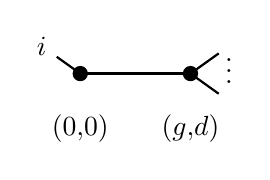
\begin{tikzpicture}[scale=0.7, baseline=-3pt,label distance=0.3cm,thick,
    virtnode/.style={circle,draw,scale=0.5}, 
    nonvirt node/.style={circle,draw,fill=black,scale=0.5} ]
    \node [nonvirt node,label=below:$(0{,}0)$] (A) {};
    \node at (2,0) [nonvirt node,label=below:$(g{,}d)$] (B) {};
    \draw [-] (A) to (B);
    \node at (-.7,.5) (n1) {$i$};
    \draw [-] (A) to (n1);
    \node at (2.7,.5) (m1) {};
    \node at (2.7,-.5) (m2) {};
    \draw [-] (B) to (m1);
    \draw [-] (B) to (m2);    
    \node at (2.7,0.2) (m3) {$\vdots$};
    \end{tikzpicture} 
\to 
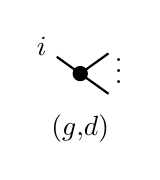
\begin{tikzpicture}[scale=0.7, baseline=-3pt,label distance=0.3cm,thick,
    virtnode/.style={circle,draw,scale=0.5}, 
    nonvirt node/.style={circle,draw,fill=black,scale=0.5} ]
    \node [nonvirt node,label=below:$(g{,}d)$] (A) {};
    \node at (-.7,.5) (n1) {$i$};
    \draw [-] (A) to (n1);
    \node at (.7,.5) (m1) {};
    \node at (.7,-.5) (m2) {};
    \draw [-] (A) to (m1);
    \draw [-] (A) to (m2);    
    \node at (.7,0.2) (m3) {$\vdots$};
    \end{tikzpicture}\ \ .
\]
\end{enumerate}
\end{lemma}
\begin{proof} 
%(1) Straightforward to check. \jocomment{I think (1) is not true, or is it? I would think that $(\sourcemap)^*[\Picabs_{\Gamma_{\delta}}]$ is the union over all $\frak N_{\Gamma_\delta \to \tilde \Gamma_\delta}$ for partial stabilizations $\Gamma_\delta \to \tilde \Gamma_\delta$. But I also think we won't need (1) below.}\textcolor{brown}{Y. Yes, you are completely right. I will remove it.}

\noindent(i) There are two pairs of universal curves with line bundle $(\frak C,\frak L)$ and $(\frak C', \frak L')$
\begin{center}
\begin{tikzcd}
\frak C' \arrow[dr,"\pi'"] \arrow[rr, "f"]
&~
& \frak C \arrow[dl,"\pi"] \\
~
&\frak N_{g,n,d}
&~
\end{tikzcd}
\end{center}
over the stack $\frak{N}_{g,n,d}$ with sections $\sigma_i:\frak N_{g,n,d}\to\frak C$ and $\sigma_i':\frak N_{g,n,d}\to \frak C'$. Because $f_*[\frak C'] = [\frak C]$, we have
\[
\targetmap^*\eta = \pi_*(c_1(\frak L)^2) = \pi_*(c_1(\frak L)^2f_*[\frak C']) = \pi'_*(c_1(f^*\frak L)^2) = (\sourcemap)^*\eta\, .
\]

\noindent (ii) Let $D'_0$ be the divisor
\[
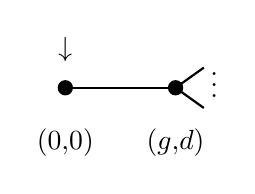
\begin{tikzpicture}[scale=0.7, baseline=-3pt,label distance=0.3cm,thick,
    virtnode/.style={circle,draw,scale=0.5}, 
    nonvirt node/.style={circle,draw,fill=black,scale=0.5} ]
    \node [nonvirt node,label=below:$(0{,}0)$] (A) {};
    \node at (2,0) [nonvirt node,label=below:$(g{,}d)$] (B) {};
    \draw [-] (A) to (B);
    %\node at (-.7,.5) (n1) {$i$};
    %\draw [-] (A) to (n1);
    \node at (0,.7) (n2) {$\downarrow$};
    \node at (2.7,.5) (m1) {};
    \node at (2.7,-.5) (m2) {};
    \draw [-] (B) to (m1);
    \draw [-] (B) to (m2);    
    \node at (2.7,0.2) (m3) {$\vdots$};
    \end{tikzpicture} 
\to 
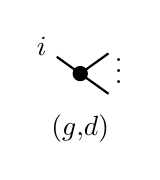
\begin{tikzpicture}[scale=0.7, baseline=-3pt,label distance=0.3cm,thick,
    virtnode/.style={circle,draw,scale=0.5}, 
    nonvirt node/.style={circle,draw,fill=black,scale=0.5} ]
    \node [nonvirt node,label=below:$(g{,}d)$] (A) {};
    \node at (-.7,.5) (n1) {$i$};
    \draw [-] (A) to (n1);
    \node at (.7,.5) (m1) {};
    \node at (.7,-.5) (m2) {};
    \draw [-] (A) to (m1);
    \draw [-] (A) to (m2);    
    \node at (.7,0.2) (m3) {$\vdots$};
    \end{tikzpicture}
\]
% \[
% \begin{tikzpicture}[scale=0.7, baseline=-3pt,label distance=0.3cm,thick,
%     virtnode/.style={circle,draw,scale=0.5}, 
%     nonvirt node/.style={circle,draw,fill=black,scale=0.5} ]
%     \node [nonvirt node,label=below:$(0{,}0)$] (A) {};
%     \node at (2,0) [nonvirt node,label=below:$(g{,}d)$] (B) {};
%     \node at (2,.7) (n1) { $\downarrow$};
%     \draw [-] (A) to (B);
%     \node at (2.7,.5) (m1) {};
%     \node at (2.7,-.5) (m2) {};
%     \draw [-] (B) to (m1);
%     \draw [-] (B) to (m2);    
%     \node at (2.7,0.2) (m3) {$\vdots$};
%     \end{tikzpicture} 
% \]
in $\frak C'$, and let $D'_i$ be the divisor
\[
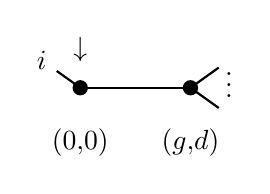
\begin{tikzpicture}[scale=0.7, baseline=-3pt,label distance=0.3cm,thick,
    virtnode/.style={circle,draw,scale=0.5}, 
    nonvirt node/.style={circle,draw,fill=black,scale=0.5} ]
    \node [nonvirt node,label=below:$(0{,}0)$] (A) {};
    \node at (2,0) [nonvirt node,label=below:$(g{,}d)$] (B) {};
    \draw [-] (A) to (B);
    \node at (-.7,.5) (n1) {$i$};
    \draw [-] (A) to (n1);
    \node at (0,.7) (n2) {$\downarrow$};
    \node at (2.7,.5) (m1) {};
    \node at (2.7,-.5) (m2) {};
    \draw [-] (B) to (m1);
    \draw [-] (B) to (m2);    
    \node at (2.7,0.2) (m3) {$\vdots$};
    \end{tikzpicture} 
\to 
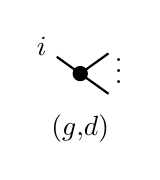
\begin{tikzpicture}[scale=0.7, baseline=-3pt,label distance=0.3cm,thick,
    virtnode/.style={circle,draw,scale=0.5}, 
    nonvirt node/.style={circle,draw,fill=black,scale=0.5} ]
    \node [nonvirt node,label=below:$(g{,}d)$] (A) {};
    \node at (-.7,.5) (n1) {$i$};
    \draw [-] (A) to (n1);
    \node at (.7,.5) (m1) {};
    \node at (.7,-.5) (m2) {};
    \draw [-] (A) to (m1);
    \draw [-] (A) to (m2);    
    \node at (.7,0.2) (m3) {$\vdots$};
    \end{tikzpicture}
\]
% \[
% \begin{tikzpicture}[scale=0.7, baseline=-3pt,label distance=0.3cm,thick,
%     virtnode/.style={circle,draw,scale=0.5}, 
%     nonvirt node/.style={circle,draw,fill=black,scale=0.5} ]
%     \node [nonvirt node,label=below:$(0{,}0)$] (A) {};
%     \node at (2,0) [nonvirt node,label=below:$(g{,}d)$] (B) {};
%     \draw [-] (A) to (B);
%     \node at (-.7,.5) (n1) {$i$};
%     \draw [-] (A) to (n1);
%     \node at (2,.7) (n2) {$\downarrow$};
%     \node at (2.7,.5) (m1) {};
%     \node at (2.7,-.5) (m2) {};
%     \draw [-] (B) to (m1);
%     \draw [-] (B) to (m2);    
%     \node at (2.7,0.2) (m3) {$\vdots$};
%     \end{tikzpicture}
% \]
in $\frak C'$. Here, the arrows pointing to the vertices with genus and degree $0$ indicate which component of the universal curve over the corresponding boundary divisor in $\frak N_{g,n,d}$ we take. The divisors $D_0', D_1', \ldots, D_n'$ are precisely the divisorial loci in $\frak C'$ which are contracted by the map $f: \frak C' \to \frak C$.
Then 
\[
\targetmap^*\psi_i = c_1(\sigma_i^*\omega_\pi)= ({\sigma}_i')^*c_1(f^*\omega_\pi) = ({\sigma}_i')^* c_1(\omega_{\pi'}(-D'_0-\sum_{i=1}^n D'_i)) = (\sourcemap)^*\psi_i - D_i\, , 
\] 
where the sections are denoted by $\sigma_i$.
\end{proof}


For the morphism $\sourcemap$, form the  fibre diagram 
\begin{equation} \label{eqn:frakNdiagrampprime}
\begin{tikzcd}
  \Picabs'_{\Gamma_{\delta}}\arrow[d]\arrow[r,"J'_{\Gamma_{\delta}}"] & \frak N\arrow[d,"\sourcemap"]\\
\Picabs_{\Gamma_{\delta}}\ar[r,"j_{\Gamma_{\delta}}"] & \Picabs_{g,0,0}. 
\end{tikzcd}
\end{equation}
By definition, the fibre product $\Picabs'_{\Gamma_{\delta}}$ parametrizes data
\[(C_v')_{v \in \V(\Gamma)}\, , \,\, \ca L'/C'=\sqcup_v C_v'\, , \,\, f: C' \to C\, , \,\, \ca L/C\, , \,\, f^* \ca L \xrightarrow{\sim} \ca L'\]
which simplifies to
\[(C_v')_{v \in \V(\Gamma)}\, , \,\, f: \sqcup_v C_v' = C' \to C\, , \,\, \ca L/C\, .\]
On the other hand, the stack $\frak N_{\Gamma_\delta}'$   parametrizes
\[
(C_v)_{v\in \V(\Gamma)}\, , \,\, \ca L/C\, , \,\, (f_v:C'_v\to C_v)_{v\in \V(\Gamma)}\, .
\]
There is a subtle difference here. For $\Picabs'_{\Gamma_{\delta}}$, the map $f$ is allowed to contract entire components $C_v'$ to points, whereas in the second case the target $C_v$ is always still 1-dimensional.


Our next step is to show 
\begin{equation} \label{eqn:Picabsprimeiso}
\Picabs'_{\Gamma_{\delta}} \cong \sqcup_{\Gamma_{\delta}\to \tilde{\Gamma}_{\delta}} \frak N_{\Gamma_{\delta}\to \tilde{\Gamma}_{\delta}}\, .\end{equation}
More precisely,
the connected components of $\Picabs'_{\Gamma_{\delta}}$ are in bijective correspondence to partial stabilizations $$\Gamma_{\delta}\to\tilde{\Gamma}_{\delta}\, .$$
We will prove, given a vertex $v \in \V(\Gamma)$ which can be contracted (with $g(v)=0$, $n(v) \leq 2$, $\delta(v)=0$), that
the locus of points in $\Picabs'_{\Gamma_{\delta}}$ where $f: C' \to C$ contracts $C_v'$ is open and closed.

For a vertex $v$ with $n(v)=2$, the universal curve $\frak C_v' \to \Picabs'_{\Gamma_{\delta}}$ has two sections (corresponding to the half-edges at $v$), and the locus where $C_v'$ is contracted equals the locus where the sections coincide, which is closed since $\frak C_v' \to \Picabs'_{\Gamma_{\delta}}$ is separated. 

To show closedness of the locus where $C_v'$ is \emph{not} contracted, assume we have a family 
\[(C_{v,S}')_{v \in \V(\Gamma)}\, , \,\, f: \sqcup_v C_{v,S}' = C_S' \to C_S\, , \,\, \ca L/C_S\, \]
of $\Picabs'_{\Gamma_{\delta}}$ over the spectrum $S$ of a strictly henselian DVR such that the fibre $C'_{v,\eta}$ of $C'_{v,S}$ over the generic point $\eta$ of $S$ is not contracted by $f$. We want to show that then also the fibre $C'_{v,L}$ over the closed point $L$ of $S$ is not contracted. By assumption,  $C'_{v,\eta}$ maps to a union $C_{v,\eta}$ of components of the fibre $C_\eta$ of $C_S$ over $\eta$. Then $C_{v,\eta}$ specializes to a union $C_{v,L}$ of components of $C_L$. Since $f$ is proper, $f$ maps the closure $C'_{v,S}$ of $C'_{v,\eta}$ to the closure of its image $C_{v,\eta}$. Since $C_{v,L}$ is still positive-dimensional, the curve $C'_{v,L}$ is indeed not contracted. For related arguments, see the proof of \cite[Proposition 2.2]{Kresch2013Flattening-stra}. 

% Younghan and I were stuck on showing that its complement is closed. This should be implied if we show that for a DVR $R$ (with closed point $L$ and open point $\eta$) and an $R$-point of $\Picabs'_{\Gamma_{\delta}}$ such that $C_{v,\eta}'$ is not contracted under $f$, then also $C_{v,L}'$ is not contracted. This seems very plausible: we can assume that the image $C_{v,\eta}$ of $C_{v,\eta}'$ under $f$ is a component of the flat map $C_\eta \to \on{Spec}(R)$ and it seems like its closure should not be a allowed to have a single point (the image of the contracted $C_{v,L}'$) as its specialization over $L$. Someone with basic knowledge of algebraic geometry to the rescue??

For a vertex $v$ with $n(v)=1$, the universal curve $\frak C_v' \to \Picabs'_{\Gamma_{\delta}}$ has a single section $\sigma_h$. On the one hand, the locus where $C_v'$ is contracted is exactly the locus where $f : \frak C' \to \frak C$ maps $\sigma_h$ to the smooth locus of $\frak C \to \Picabs'_{\Gamma_{\delta}}$, thus it is open. On the other hand, it is also the preimage under $\sigma_h$ of the exceptional locus of $\frak C' \to \frak C$, and thus closed.

We have proven that the connected components of $\Picabs'_{\Gamma_{\delta}}$ are in bijective correspondence to partial stabilizations $\Gamma_{\delta}\to\tilde{\Gamma}_{\delta}$. But a point 
\[(C_v')_{v \in \V(\Gamma)}\, , \,\, f: \sqcup_v C_v' = C' \to C\, , \,\, \ca L/C\]
on the corresponding component is equivalent to the data of any collection of curves $C_v'$ for $v' \in \V(\Gamma) \setminus \V(\tilde \Gamma)$, which are contracted by $f$, together with a point
\[(C_v')_{v \in \V(\tilde \Gamma)}\, , \,\, f: (C_v' \to C_v)\, , \,\, \ca L/C = \sqcup_{v \in V(\tilde \Gamma)} C_v\]
of $\frak N'_{\Tilde{\Gamma}_{\delta}}$. Hence, we have a isomorphism
\[\frak N_{\Gamma_{\delta}\to \tilde{\Gamma}_{\delta}} \cong \frak N'_{\Tilde{\Gamma}_{\delta}}\times \prod_{v\in \V(\Gamma)\setminus \V(\Tilde{\Gamma})} \frak M_{0,\n(v)}\, ,\]
where, in the last expression, $n(v)$ is necessarily $1$ or $2$.

% \{Maybe we want something like the following (haven't completely understood the above though). 

% Let $S$ be spec of a strictly hensellian DVR, and $f\colon C'\to C$ a map of prestable curves over $S$. Let $C_v$ be a connected component of the normalisation of $C_\eta$, with closure $\bar C_v$. Assume that $f$ is not constant on $C_v$. Then $f$ is not constant on the fibre $\bar C_v \times_S s$ (it may contract some components, but not all). 

% Proof. 
% $f$ is proper, so its image is closed, hence contains (in fact, equals) the closure of $f(C_v)$. But this is the closure of an irreducible component of a prestable curve, so its closed fibre has positive dimension. \qed
% }

For each partial stabilisation $\Gamma_{\delta}\to \tilde{\Gamma}_{\delta}$, we denote by $$J_{\Gamma_{\delta}\to\tilde{\Gamma}_{\delta}}: \frak N_{\Gamma_{\delta}\to\tilde{\Gamma}_{\delta}}\to \frak N$$ the restriction of $J'_{\Gamma_{\delta}}$ to $\frak N_{\Gamma_{\delta}\to \tilde{\Gamma}_{\delta}}$.  
\begin{lemma}\label{lem:N_invariance_P}
We have $\targetmap^* \P_{g}^\bullet = (\sourcemap)^* \P_g^\bullet
\, \in\, \prod_{c=0}^\infty {\mathsf{CH}}^c_{\mathsf{op}}(\frak N)$
for all $c \geq 0$. 
\end{lemma}
\begin{proof} 
We will use  formula \eqref{eqn:P_gformula2}
for $\P_g^\bullet$. By \cref{lem:pullback_comparison}, the terms $\exp(- \eta/2)$ have identical pullback under $\targetmap$ and $\sourcemap$. We can therefore
focus on the sum over graphs and weighting mod $r$. 

We start with a few remarks about the combinatorial factors in $\P_g^\bullet$ which will arise in the proof. Let $\Gamma_{\delta}\to\tilde{\Gamma}_{\delta}$ be a partial stabilization, then the Betti numbers agree,
$$h^1(\Gamma_\delta) = h^1(\tilde \Gamma_\delta)\, .$$
Given $r$, the map $W_{\Gamma_\delta,r} \to W_{\tilde \Gamma_\delta, r}$ of admissible weightings mod $r$ (induced by the inclusion $H(\tilde \Gamma) \to H(\Gamma)$ of half-edge sets) is a bijection. 

Moreover, if the map $\Gamma_{\delta}\to\tilde{\Gamma}_{\delta}$ only contracts components with $$(\g(v),\n(v),\delta(v))=(0,2,0)\,,$$ there is a canonical isomorphism $\Aut(\Gamma_\delta) \cong \Aut(\tilde \Gamma_\delta)$. On the other hand, in the formula for $\P_g^\bullet$, every term such that $\Gamma_\delta$ has a vertex with $$(\g(v), \n(v), \delta(v))=(0,1,0)$$ necessarily vanishes. Indeed, the half-edge $h$ at this vertex must have $w(h)=0$ such that the corresponding edge term vanishes. 

To keep the notation concise, we write $\Phi_{a}$ for the power-series 
\begin{align*} 
\Phi_{a}(x)&= \frac{1-\exp({-\frac{a}{2}}x)}{x}\\ &= \sum_{m=0}^\infty (-1)^m (\frac{a}{2})^{m+1} \frac{1}{(m+1)!}x^m = \frac{a}{2} - \frac{a^2}{8} x + \ldots 
\end{align*}
appearing in the edge terms of $\P_g^\bullet$. Moreover, given a graph $\tilde \Gamma_\delta$ with a half-edge $h$ incident to a vertex $v$, denote by $\psi_h, \psi_h'$ the classes on $\frak N'_{\tilde \Gamma_\delta}$ pulled back from $\frak N_{\g(v),\n(v),\delta(v)}$ in the diagram \eqref{eqn:frakNdiagramp}. Similarly, given a partial stabilization $\Gamma_\delta \to \tilde \Gamma_\delta$, the space $\frak N_{\Gamma_\delta \to \tilde \Gamma_\delta}$ contains $\frak N'_{\tilde \Gamma_\delta}$ as a factor, hence the notation also makes sense on $\frak N_{\Gamma_\delta \to \tilde \Gamma_\delta}$ (provided $h$ is a half-edge of $\tilde \Gamma_\delta$).

Let us first compute the pullback of the graph sum in $\P_g^{\bullet,r}$ via $\sourcemap : \frak N \to \Picabs_{g,0,0}$. Using the diagram \eqref{eqn:frakNdiagrampprime} and the decomposition \eqref{eqn:Picabsprimeiso}, we see
\begin{align} 
&(\sourcemap)^* \sum_{\Gamma_\delta, w}
\frac{r^{-h^1( \Gamma_\delta)}}{|\Aut(\Gamma_\delta)| }
\;
j_{\Gamma_\delta*}\Bigg[
\prod_{e=(h,h')\in \E(\Gamma_\delta)}
\Phi_{w(h)w(h')}(\psi_h + \psi_{h'}) \Bigg] \nonumber\\
=&\sum_{\Gamma_\delta \to \tilde \Gamma_\delta, w} \label{eqn:pprimepullb}
\frac{r^{-h^1( \Gamma_\delta)}}{|\Aut(\Gamma_\delta)| }
\;
J_{\Gamma_\delta \to \tilde \Gamma_\delta*}\Bigg[
\prod_{e=(h,h')\in \E(\Gamma_\delta)}
\Phi_{w(h)w(h')}(\psi'_h + \psi'_{h'}) \Bigg]\, .
\end{align}
In the second line, the sum is over all partial stabilizations $\Gamma_\delta \to \tilde \Gamma_\delta$.

Second, we compute the pullback of the graph sum in $\P_g^{\bullet,r}$ via $\targetmap : \frak N \to \Picabs_{g,0,0}$
\begin{align} 
&\targetmap^* \sum_{\tilde \Gamma_\delta, w}
\frac{r^{-h^1(\tilde  \Gamma_\delta)}}{|\Aut(\tilde \Gamma_\delta)| }
\;
j_{\tilde \Gamma_\delta*}\Bigg[
\prod_{e=(h,h')\in \E(\tilde \Gamma_\delta)}
\Phi_{w(h)w(h')}(\psi_h + \psi_{h'}) \Bigg]\nonumber \\
=&\sum_{\tilde \Gamma_\delta, w}\label{eqn:ppullb}
\frac{r^{-h^1(\tilde \Gamma_\delta)}}{|\Aut(\tilde \Gamma_\delta)| }
\;
\widehat J_{\tilde \Gamma_\delta*}\Bigg[
\prod_{e=(h,h')\in \E(\tilde \Gamma_\delta)}
\Phi_{w(h)w(h')}(\psi_h + \psi_{h'}) \Bigg]\, .
\end{align}
We use here the right fibre diagram in \eqref{eqn:frakNdiagramp} together with the fact that $G$ is proper, representable, and birational.  So by Proposition \ref{prop:invarianceproperbirat},
the pushforward of fundamental classes under $J_{\tilde \Gamma_\delta}$ and $\widehat J_{\tilde \Gamma_\delta}$ agree.

To compare to the formula for the pullback under $\sourcemap$, we use 
$$\psi_h + \psi_{h'} = \psi_h' - D_h + \psi_{h'}'- D_{h'}$$ on $\frak N'_{\tilde \Gamma_\delta}$ by \cref{lem:pullback_comparison}.
%By \cref{lem:pullback_comparison}, it is enough to show that the pullback of each edge term along $\targetmap$ and $\sourcemap$ coincide. For simplicity, we introduce a function $\Phi_{e,w}(x)= \frac{1-\exp({-\frac{w(h)w(h')}{2}}x)}{x}$ for each edge $e=(h,h')$. 
The next step of the proof is to use the self-intersection formula for $D_h, D_{h'}$ (similar to the formula described in \cite[Appendix A]{GraberPandharipande}) to expand the edge term
\[\Phi_{w\,w'}(\psi_h' - D_h + \psi_{h'}'- D_{h'}) = \sum_{m=0}^\infty (-1)^m (\frac{w\,w'}{2})^{m+1} \frac{1}{(m+1)!}(\psi_h' - D_h + \psi_{h'}'- D_{h'})^m.\] For example, $(D_h)^2$ is equal to
\begin{equation*}
-
    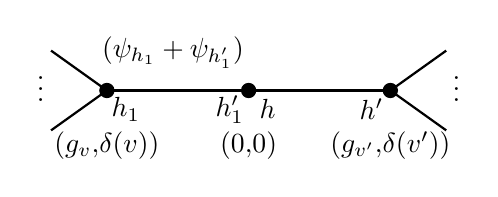
\begin{tikzpicture}[scale=1.2, baseline=-3pt,label distance=0.3cm,thick,
    virtnode/.style={circle,draw,scale=0.5}, 
    nonvirt node/.style={circle,draw,fill=black,scale=0.5} ]
    \node at (0,0) [nonvirt node,label=below:$(g_{v}{,}\delta(v))$] (A) {};
    \node at (1.5,0) [nonvirt node,label=below:$(0{,}0)$] (C) {};    
    \node at (3,0) [nonvirt node,label=below:$(g_{v'}{,}\delta(v'))$] (B) {};
    \node at (.2,-.2) {$h_1$};
    \node at (1.3,-.2) {$h'_1$}; 
    \node at (1.7,-.2) {$h$};
    \node at (2.8,-.2) {$h'$};
    \draw [-] (A) to (C);
    \draw [-] (B) to (C);
    \node at (.7,.4) {$(\psi_{h_1}+\psi_{h'_1})$};
    \node at (3.7,.5) (m1) {};
    \node at (3.7,-.5) (m2) {};
    \draw [-] (B) to (m1);
    \draw [-] (B) to (m2);    
    \node at (3.7,0.1) (m3) {$\vdots$};
    \node at (-0.7,.5) (n1) {};
    \node at (-0.7,-.5) (n2) {};
    \draw [-] (A) to (n1);
    \draw [-] (A) to (n2);    
    \node at (-.7,0.1) (n3) {$\vdots$};    
    \end{tikzpicture}
+ \,2
    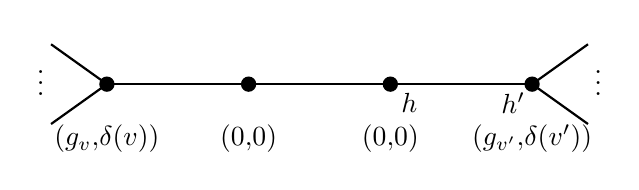
\begin{tikzpicture}[scale=1.2, baseline=-3pt,label distance=0.3cm,thick,
    virtnode/.style={circle,draw,scale=0.5}, 
    nonvirt node/.style={circle,draw,fill=black,scale=0.5} ]
    \node at (0,0) [nonvirt node,label=below:$(g_{v}{,}\delta(v))$] (A) {};
    \node at (1.5,0) [nonvirt node,label=below:$(0{,}0)$] (C) {};   
    \node at (3,0) [nonvirt node,label=below:$(0{,}0)$] (D) {}; 
    \node at (4.5,0) [nonvirt node,label=below:$(g_{v'}{,}\delta(v'))$] (B) {};
    \node at (3.2,-.2) {$h$};
    \node at (4.3,-.2) {$h'$};
    \draw [-] (A) to (C);
    \draw [-] (C) to (D);
    \draw [-] (D) to (B);
    \node at (5.2,.5) (m1) {};
    \node at (5.2,-.5) (m2) {};
    \draw [-] (B) to (m1);
    \draw [-] (B) to (m2);    
    \node at (5.2,0.1) (m3) {$\vdots$};
    \node at (-0.7,.5) (n1) {};
    \node at (-0.7,-.5) (n2) {};
    \draw [-] (A) to (n1);
    \draw [-] (A) to (n2);    
    \node at (-.7,0.1) (n3) {$\vdots$};    
    \end{tikzpicture}
\end{equation*}
and similarly for $(D_{h'})^2$.

The result will be a linear combination of terms
\begin{equation}
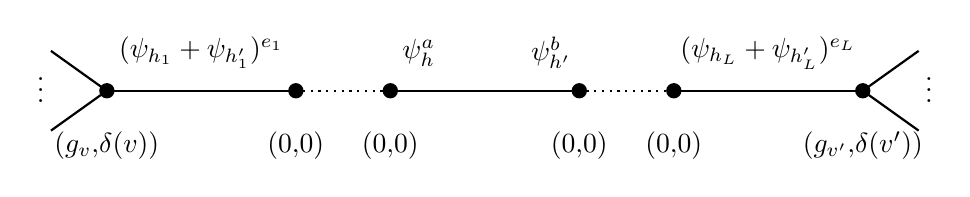
\begin{tikzpicture}[scale=1.2, baseline=-3pt,label distance=0.3cm,thick,
    virtnode/.style={circle,draw,scale=0.5}, 
    nonvirt node/.style={circle,draw,fill=black,scale=0.5} ]
    \node at (-6,0) [nonvirt node,label=below:$(g_{v}{,}\delta(v))$] (F) {};
    \node at (-4,0) [nonvirt node,label=below:$(0{,}0)$] (E) {};
    \node at (-3,0) [nonvirt node,label=below:$(0{,}0)$] (D) {};
    \node at (-1,0) [nonvirt node,label=below:$(0{,}0)$] (C) {};
    \node [nonvirt node,label=below:$(0{,}0)$] (A) {};
    \node at (2,0) [nonvirt node,label=below:$(g_{v'}{,}\delta(v'))$] (B) {};
    \draw [-] (A) to (B);
    \draw [-, dotted] (C) to (A);
    \draw [-] (D) to (C);
    \draw [-, dotted] (E) to (D);
    \draw [-] (F) to (E);
    \node at (1,.4) {$(\psi_{h_L}+\psi_{h'_L})^{e_L}$};
    \node at (-5,.4) {$(\psi_{h_1}+\psi_{h'_1})^{e_1}$};
    \node at (-2.7,.4) {$\psi_h^a$};
    \node at (-1.3,.4) {$\psi_{h'}^b$};
    %\node at (-.7,.5) (n1) {$i$};
    %\draw [-] (A) to (n1);
    %\node at (0,.7) (n2) {$\downarrow$};
    \node at (2.7,.5) (m1) {};
    \node at (2.7,-.5) (m2) {};
    \draw [-] (B) to (m1);
    \draw [-] (B) to (m2);    
    \node at (2.7,0.1) (m3) {$\vdots$};
    \node at (-6.7,.5) (n1) {};
    \node at (-6.7,-.5) (n2) {};
    \draw [-] (F) to (n1);
    \draw [-] (F) to (n2);    
    \node at (-6.7,0.1) (n3) {$\vdots$};    
    \end{tikzpicture}
\end{equation}
where the edge $(h,h')$ is at position $\ell$ in the above chain ($1 \leq \ell \leq L$). The total degree of this term (before the pushforward by $\widehat J_{\tilde \Gamma_\delta}$) is
\[m = \sum_{j \neq \ell} (e_j+1) + a + b\, .\]
The total coefficient of this particular term in $\Phi_{w\,w'}(\psi_h' - D_h + \psi_{h'}'- D_{h'})$ is then
\[
%\mathrm{Coeff} = 
\underbrace{(-1)^m (\frac{w\,w'}{2})^{m+1} \frac{1}{(m+1)!}}_{\text{coeff in $\Phi_{w\,w'}$}}\cdot \binom{m}{e_1+1, \ldots, a,b,\ldots, e_L+1} \underbrace{(-1)^{L-1}}_{\substack{\text{excess intersection}\\\text{of $-D_h, -D_{h'}$}}} % \underbrace{(-1)^{\sum_{j \neq i} e_j+1}}_{\text{sign from $-D_h, -D_{h'}$}} \cdot \underbrace{(-1)^{\sum_{j \neq i} e_j}}_{\text{excess intersection}},
\]
where the multinomial coefficient comes from the expansion of $$(\psi_h' - D_h + \psi_{h'}'- D_{h'})^m\, .$$
Writing $e_\ell=a+b$, we can simplify to obtain
\[
%\mathrm{Coeff} = 
\frac{1}{m+1}
\left(\prod_{j=1}^L (-1)^{e_j} (\frac{w\,w'}{2})^{e_j+1} \frac{1}{(e_j+1)!} \right) \binom{e_\ell}{a} (e_\ell+1)\, .
\]
Summing over all choices $a+b=e_\ell$ for fixed $e_\ell$, the coefficient of the term
\begin{equation}
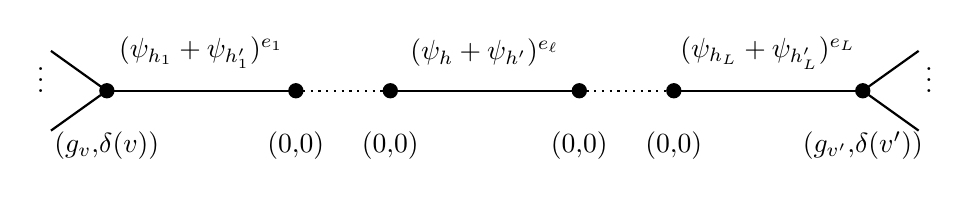
\begin{tikzpicture}[scale=1.2, baseline=-3pt,label distance=0.3cm,thick,
    virtnode/.style={circle,draw,scale=0.5}, 
    nonvirt node/.style={circle,draw,fill=black,scale=0.5} ]
    \node at (-6,0) [nonvirt node,label=below:$(g_{v}{,}\delta(v))$] (F) {};
    \node at (-4,0) [nonvirt node,label=below:$(0{,}0)$] (E) {};
    \node at (-3,0) [nonvirt node,label=below:$(0{,}0)$] (D) {};
    \node at (-1,0) [nonvirt node,label=below:$(0{,}0)$] (C) {};
    \node [nonvirt node,label=below:$(0{,}0)$] (A) {};
    \node at (2,0) [nonvirt node,label=below:$(g_{v'}{,}\delta(v'))$] (B) {};
    \draw [-] (A) to (B);
    \draw [-, dotted] (C) to (A);
    \draw [-] (D) to (C);
    \draw [-, dotted] (E) to (D);
    \draw [-] (F) to (E);
    \node at (1,.4) {$(\psi_{h_L}+\psi_{h'_L})^{e_L}$};
    \node at (-5,.4) {$(\psi_{h_1}+\psi_{h'_1})^{e_1}$};
    \node at (-2,.4) {$(\psi_{h}+\psi_{h'})^{e_\ell}$};
    %\node at (-.7,.5) (n1) {$i$};
    %\draw [-] (A) to (n1);
    %\node at (0,.7) (n2) {$\downarrow$};
    \node at (2.7,.5) (m1) {};
    \node at (2.7,-.5) (m2) {};
    \draw [-] (B) to (m1);
    \draw [-] (B) to (m2);    
    \node at (2.7,0.2) (m3) {$\vdots$};
    \node at (-6.7,.5) (n1) {};
    \node at (-6.7,-.5) (n2) {};
    \draw [-] (F) to (n1);
    \draw [-] (F) to (n2);    
    \node at (-6.7,0.2) (n3) {$\vdots$};    
    \end{tikzpicture}
\end{equation}
is exactly equal to
\[
%\mathrm{Coeff} = 
\frac{e_\ell +1}{m+1}
\left(\prod_{j=1}^L (-1)^{e_j} (\frac{w\,w'}{2})^{e_j+1} \frac{1}{(e_j+1)!} \right).
\]
Pushing forward by $\widehat J_{\tilde \Gamma_\delta}$, we forget where in the chain above the edge $(h,h')$ has been. Summing over the $L$ possible positions and using $m+1 = \sum_{\ell=1}^L (e_\ell +1)$, we obtain the coefficient
\[\prod_{j=1}^L \underbrace{(-1)^{e_j} (\frac{w\,w'}{2})^{e_j+1} \frac{1}{(e_j+1)!}}_{\text{coefficient of $x^{e_j}$ in $\Phi_{w\,w'}(x)$}}\, .\]
From the above discussion, we see that \eqref{eqn:ppullb} equals
\[\sum_{\Gamma_\delta \to \tilde \Gamma_\delta, w}
\frac{r^{-h^1( \tilde \Gamma_\delta)}}{|\Aut(\tilde \Gamma_\delta)| }
\;
J_{\Gamma_\delta \to \tilde \Gamma_\delta*}\Bigg[
\prod_{e=(h,h')\in \E(\Gamma_\delta)}
\Phi_{w(h)w'(h)}(\psi'_h + \psi'_{h'}) \Bigg]\, .\]
%Here, a priori 
The sum goes over stabilizations $\Gamma_\delta \to \tilde \Gamma_\delta$ contracting chains of curves with $(g,n,d)=(0,2,0)$.
By the previous remarks concerning the combinatorial factors, we have
\[h^1( \tilde \Gamma_\delta) = h^1(\Gamma_\delta)\, , \ \ \ |\Aut(\tilde \Gamma_\delta)| = |\Aut(\Gamma_\delta)|\, . \]
The sum does not change if we allow arbitrary stabilizations $\Gamma_\delta \to \tilde \Gamma_\delta$, since for $\Gamma_\delta$ having a vertex with $(g,n,d)=(0,1,0)$, the summand automatically vanishes. Thus the sum above equals the term computed in \eqref{eqn:pprimepullb}. 
% We first prove the case when $\E(\Gamma)=\{e=(h,h')\}$ with weight $w$. For each partial stabilization $\hat{\Gamma}_{\delta}\to \Gamma_{\delta}$, there exists a unique weighting $\hat{w}$ on $\hat{\Gamma}_{\delta}$ with $\hat{w}(h)=w(h)$ and $\hat{w}(h')=w(h')$. Then 
% \begin{equation*}
% \begin{split}
% \targetmap^*j_{\Gamma_{\delta}*}\Phi_{e,w}(\psi_h+\psi_{h'}) &= J_{\Gamma_{\delta}*}\targetmap^*\Phi_{e,w}(\psi_h+\psi_{h'}) \\
% &=J_{\Gamma_{\delta}*}\Phi_{e,w}((\sourcemap)^*(\psi_h+\psi_{h'})-D_h-D_{h'})\\
% &= ... \\
% &=\sum_{\hat{\Gamma}_{\delta}\to\Gamma_{\delta}}J'_{\hat{\Gamma}_{\delta}\to\Gamma_{\delta}*}\prod_{e\in\E(\hat{\Gamma})}\Phi_{e,\hat{w}}((\sourcemap)^*(\psi_h+\psi_{h'}))\\
% &=\sum_{\hat{\Gamma}_{\delta}\to\Gamma_{\delta}}(\sourcemap)^* J_{\hat{\Gamma}_{\delta}\to\Gamma_{\delta}*}\prod_{e\in\E(\hat{\Gamma})}\Phi_{e,\hat{w}}(\psi_h+\psi_{h'})\\
% &=\sum_{\hat{\Gamma}_{\delta}}(\sourcemap)^*j_{\hat{\Gamma}_{\delta}*}\prod_{e\in\E(\hat{\Gamma})}\Phi_{e,\hat{w}}(\psi_h+\psi_{h'})
% \end{split}
% \end{equation*}
% where $\hat{\Gamma}_{\delta}\to\Gamma_{\delta}$ is all partial stabilization. The third equality comes from the excess intersection formula of $(D_h)^k$. For general graph $\Gamma_{\delta}$, we can use the formula above at each edge. 
\end{proof}
%Now we show \cref{eq:pullback_pixton}, continuing in the notation we just set up. Choose a vector of integers $A=(\bd 0, a_{n+1},\cdots,a_{n+m})\in \mathbb{Z}^{n+m}$ such that $\ca L'(AP)$ is relatively very ample. Let $p\colon U_{l}'\to B'$ be the scheme over $B'$ constructed in \cref{sec:very_ample}.  Consider the following diagram
%\begin{equation}
% \begin{tikzcd}
%  U'_l \arrow[r, "\phi_{\ca L'(AP)}"]\arrow[d, "p"]& \overline{\mathcal{M}}_{g,n+m}(X,\beta) \arrow[d, "\phi_{f^*\ca O(1)\otimes(-AP)}"] \\
%  B' \arrow[r, "\ca \phi_{\ca L'}"]\arrow[d, "h"]\arrow[dr, "\phi_{\ca L'}"] & \Picabs_{g,n+m} \arrow[d]\\
%  B \arrow[r, "\phi_{\ca L}"]  & \Picabs_{g,n}.
%\end{tikzcd}
%\end{equation}
%where the lower left corner is not commutative. Since the pull back along $p$ is injective, it is enough to prove \cref{eq:pullback_pixton} on $U_{l}'$. In principle, 
%$\phi_{\ca L}^*\P_{g,\bd 0,0}^g(h \circ p)$ has all contributions from some chains of $\bb P^1$s which was inserted. After restricting to $\Picabs'$, contributions from $\bb P^1$ chains where line bundle has degree $0$ vanishes. 
%On the other hand, $\phi_{\ca L'(AP)} : U_{l}'\to \Picabs_{g,n+m}$ factors through $\overline{\mathcal{M}}_{g,n+m}(X,\beta)$, so on the unstable locus, the degree of the line bundle should be positive. Therefore we do not have contributions from $\PP^1$ chains with degree $0$. 
%=========

%I think the advantage for the proof of invariance under $\Phi$ is that it plays out purely on $\Picabs_{g,n,d}$ and not some strange family parametrized by $B$. For the vertex term $\exp(- \eta/2)$ this will be a standard computation involving the fact that the map $\frak C' \to \frak C$ is birational, thus fundamental class pushes forward to fundamental class. For the sum over graphs, I think there will be natural diagrams
%\[
%\begin{tikzcd}
%\prod_{v \in \V(\Gamma)} \Picabs_{g(v),n(v),\delta(v)} \arrow[d,"\prod_v \Phi_i"] &\Picabs_{\Gamma_{\delta}} \arrow[l] \arrow[r] \arrow[d] & \Picabs_{g,n,0} \arrow[d,"\Phi"]\\
%\prod_{v \in \V(\Gamma)} \Picabs_{g(v),n(v),\delta(v)} &\Picabs_{\Gamma_{\delta}} \arrow[l]\arrow[r] & \Picabs_{g,n,0}
%\end{tikzcd}
%\]
%for $\Gamma_\delta$ not containing a vertex of type $(g,n,d)=(0,0,0)$ (otherwise the fibre product is a bit strange - the generic point has no preimage, but if the $(0,0,0)$-curve degenerates into a $(0,0,a)$ and a $(0,0,-a)$-curve, then it can suddenly have preimages ... to think about). The right square is cartesian (maybe the left too). 

%Are these ingredients enough to show the invariance? I think the terms $\psi_h + \psi_{h'}$ will pull back to themselves \emph{plus} a contribution from inserting an unstable $(g,n,d)=(0,0,0)$-bubble inside the half-edge, and this turns out to be compatible with Pixton's formula?




%, because in the situation of invariance \invnrIV{} we essentially say that we are given a $\ca S$-point of $\ca N$ and then show an equality of operational classes on $\ca S$ pulled back from $\Picabs_{g,0,0}$ via $p,\sourcemap$.
%\{This I completely agree with, and it gives a good perspective on Inv IV. }

%But my hope would be that $\ca N$ exists and that one can do tautological computations on it. Also, I am guessing that the pullbacks of $\aj : \cat{Div}_g \to \Picabs_{g,0,0}$ via the two maps $p,\sourcemap$ should be isomorphic by the same arguments that David wrote before.

%\begin{proof}[Proof of Invariance \invnrIV{}]
%%This invariance is exactly what is shown in the proof of Lemma \ref{Lem:DR_alteration_invar}, and more precisely in \eqref{eq:pullback_pixton} and \eqref{eq:pullback_Div}.
%The data in the situation of Invariance \invnrIV{} give us exactly a map $\ca S \to \frak N$, and the invariance is immediate from \cref{lem:N_invariance_DR} (on the operational side), and from \cref{lem:N_invariance_P} (on the Pixton side). 
%% we essentially say that we are given a $\ca S$-point of $\ca N$ and then show an equality of operational classes on $\ca S$ pulled back from $\Picabs_{g,0,0}$ via $p,\sourcemap$.
%\end{proof}
%\appendix


%\section{Prestable curves and log curves}\label{sec:prestable_vs_log_curves}
%\{This section worries me slightly. It seems a convenient result, and an obvious thing to state, but I can't find it in the literature. Maybe there's some subtlety I'm missing? }
%
%Fix a genus $g$ and a number of markings $n$. We write $\frak M_{g,n}$ for the stack of prestable curves of genus $g$ with $n$ ordered smooth disjoint marked sections, and $\pi\colon \frak  C_{g,n}\to \frak M_{g,n}$ for the universal prestable curve over it, with markings $p_i$. We write $\ca M_{g,n}^{log}$ for the stack of log curves of genus $g$ with $n$ markings (see \cite{Kato2000Log-smooth-defo}), where we order the markings. The latter is shown in \cite[Theorem 3.12]{Gillam2012Logarithmic-sta} to be a groupoid fibration with log structure. In this section we equip $\frak M_{g,n}$ with the log structure coming from the boundary, and show that the resulting map $\frak M_{g,n} \to \ca M^{log}_{g,n}$ is a strict open immersion. 
%
%\begin{lemma}
%The stack $\frak M_{g,n}$ is smooth over ${\field}$, and the closed substack $\Delta$ of non-smooth curves is a normal-crossings divisor. 
%\end{lemma}
%\begin{proof}
%This is standard; the map
%\begin{equation}
%F\colon \bigsqcup_{m \ge 0} \Mbar_{g,n+m} \to \frak M_{g,n}
%\end{equation}
%forgetting the last $m$ markings is smooth and surjective, and the pullback of $\Delta$ is precisely the union of the boundaries. The result follows from the fact that being normal-crossings is a smooth-local property. 
%\end{proof}
%
%We can then equip $\frak  M_{g,n}$ with the log structure coming from this boundary, making it log smooth over ${\field}$ (equipping the latter with the trivial log structure). Unlike in the stable case, the natural map $\frak M_{g,n+1} \to \frak C_{g,n}$ is not an isomorphism, so we cannot equip $\frak C_{g,n}$ with a log structure via this map. Instead, we define a divisor $\Delta_{\frak C}$ in $\frak C_{g,n}$ as 
%\begin{equation}
%\Delta_{\frak C} = \pi^*\Delta + \sum_{i=1}^n p_i. 
%\end{equation}
%Evidently this $\Delta_{\frak C}$ is a normal crossings divisor on the smooth stack $\frak C_{g,n}$, hence defines a log structure making it log smooth over ${\field}$. The map of stacks $\pi\colon \frak C_{g,n} \to \frak M_{g,n}$ lifts uniquely to one of log stacks, since $\pi^*$ of a function which is a unit outside $\Delta$ will be a unit outside $\Delta_{\frak C}$. To see that the natural map $\pi\colon \frak C_{g,n} \to \frak M_{g,n}$ of log stacks is a log curve we just need to check that it is log smooth and integral (cf. \cite{Kato2000Log-smooth-defo}), but these are both local conditions, and our morphism is locally modelled on the standard log structure of stable curves. 
%
%%\begin{lemma}\{No, this is wrong - David to fix!}
%%Equipping $\frak M_{g, n+1}$ and $\frak M_{g,n}$ with the log structures coming from their boundaries, the map $\frak M_{g, n+1} \to \frak M_{g,n}$ (forgetting the last marking) makes $\frak M_{g, n+1}$ into a log curve over $\frak M_{g,n}$. 
%%\end{lemma}
%%\begin{proof}
%%Being a log curve is a local property for the strict smooth topology, so we can check this after pullback along $F$, whereupon it follows from \cite{Kato2000Log-smooth-defo}. 
%%\end{proof}
%%\begin{lemma}
%%The log curve $\frak C_{g,n} / \frak M_{g,n}$ of the previous lemma is \emph{basic} in the terminology of \cite[definition 3.8]{Gillam2012Logarithmic-sta}. 
%%\end{lemma}
%%\begin{proof}
%%This is again a smooth-local property, and is verified for stable curves by \cite{Kato2000Log-smooth-defo}. 
%%\end{proof}
%
%One verifies easily that the log curve $\frak C_{g,n} / \frak M_{g,n}$ is \emph{basic} in the terminology of \cite[definition 3.8]{Gillam2012Logarithmic-sta}. Gillam proves \cite[Lemma 3.10]{Gillam2012Logarithmic-sta} that basic log structures are minimal, hence the map $\phi\colon \frak M_{g,n} \to \ca M^{log}_{g,n}$ induced by this log structure is strict. 
%
%\begin{lemma}\label{lem:strict_open_immersion}
%The strict morphism $\phi\colon \frak M_{g,n} \to \ca M^{log}_{g,n}$ is an open immersion. 
%\end{lemma}
%\begin{proof}
%The map $\ul \phi$ is fully faithful, hence relatively representable by algebraic spaces, and is a monomorphism. It is also locally of finite presentation, hence relatively representable by schemes by \cite[\href{https://stacks.math.columbia.edu/tag/0B89}{Tag 0B89}]{stacks-project}. 
%
%There is a map $\psi\colon \ul{\ca M}^{log}_{g,n} \to \frak M_{g,n}$ by forgetting the log structure, and our map $\phi$ is a section of $\psi$. The map $\psi$ is birational; it is an isomorphism on the dense open locus of stable curves by \cite{Kato2000Log-smooth-defo}. Hence $\phi$ is an open immersion by \todo{D to add: lemma in paper with Sam (online soon...)}. 
%\end{proof}
%
%\begin{remark}
%I do not know whether $\phi$ is an isomorphism; I suspect not, but do not have an example to hand. It is equivalent to ask whether there exists a prestable curve over a separably closed field admitting a basic log structure other than the one coming from the above construction. Kato \cite{Kato2000Log-smooth-defo} shows this to be impossible in the stable case. 
%\end{remark}
%
%\{$\phi$ is an iso! Kato prop 2.3 doesn't use stability. This is also remarked in appendix to [Gross Siebert, log GW theory. }

%This does not prove that $\frak M_{g,n} \to \ca M^{log}_{g,n}$ is an iso, it just proves that it is a strict map. Maybe we can show that this map is also open, or something? Then I would feel better about pulling back along it... Note that there is a map the other way, and this is a section of it. And iso over DM locus. OK, we have a birational map of smooth stacks with a section. I guess image is open. I think the map is faithful, so relatively representable by algebraic spaces. And locally of finite presentation. And monomorphism. But monomorphism of algebraic spaces locally of finite type is representable by schemes by \cite[\href{https://stacks.math.columbia.edu/tag/0B89}{Tag 0B89}]{stacks-project}. Then it is open by lemma in paper with Sam. 



\section{Applications}\label{sec:applications}
\subsection{Proofs of Theorem \ref{FPA1} and Conjecture A} \label{Sect:ProofConjA}
We start by recalling notions presented in Section \ref{Sect:Twistdiffintro}, but now in the more general setting of $k$-differentials.
Let $A=(a_1,\ldots,a_n)$ be a vector of zero and pole multiplicities
satisfying
$$\sum_{i=1}^n a_i= k(2g-2)\, .$$
Let $\HH^k_g(A) \subset \mathcal{M}_{g,n}$ be the closed (generally non-proper) locus 
of pointed curves $(C,p_1,\ldots,p_n)$ satisfying the condition
$$\mathcal{O}_C\Big(\sum_{i=1}^n a_i p_i\Big) \simeq \omega_C^{\otimes k}\, .$$
In other words, $\HH^k_g(A)$ is the locus of (possibly) meromorphic $k$-differentials
with zero and pole multiplicities prescribed by $A$.
In \cite{Farkas2016The-moduli-spac}, a compact moduli space of twisted $k$-canonical divisors
$$\widetilde{\HH}^k_g(A) \subset \overline{\mathcal{M}}_{g,n}$$
is constructed extending $\HH^k_g(A) = \widetilde{\HH}^k_g(A) \cap \mathcal{M}_{g,n} $ to the boundary of $\overline{\mathcal{M}}_{g,n}$.

For $k \geq 1$ and $A$ not of the form $A = k \cdot A'$ with a vector $A'$ of nonnegative integers, the locus
$\widetilde{\HH}^k_g(A)$ is of pure codimension $g$ in
$\overline{\mathcal{M}}_{g,n}$ by \cite[Theorem 3]{Farkas2016The-moduli-spac} (for $k=1$) and \cite[Theorem 1.1]{Schmitt2016Dimension-theor} (for $k>1$). 
A weighted fundamental cycle of $\widetilde{\HH}^k_g(A)$, 
\begin{equation}\label{wwww4k}
\mathsf{H}^k_{g,A}\in \mathsf{CH}_{2g-3+n}(\oM_{g,n})\ ,
\end{equation}
is constructed in
\cite[Appendix A]{Farkas2016The-moduli-spac} and \cite[Section 3.1]{Schmitt2016Dimension-theor} with explicit nontrivial 
weights on the irreducible components.
The closure
$$\overline{\HH}^k_{g,A}\subset \oM_{g,n}$$
contributes to the weighted fundamental class $\mathsf{H}^k_{g,A}$ with
multiplicity 1, but there are additional boundary contributions, as described in the references above.

The weighted fundamental class 
$\mathsf{H}^k_{g,A}$
was conjectured in \cite{Farkas2016The-moduli-spac, Schmitt2016Dimension-theor}
to equal  the class given by Pixton's formula for the double ramification cycle. To state the conjecture, consider the shifted\footnote{The shift is needed since Pixton's original formula worked with powers of the log-canonical line bundle $\omega_C^{\text{log}} = \omega_C(\sum_{i=1}^n p_i)$ instead of $\omega_C$.} vector $\widetilde A = (a_1 + k, \ldots, a_n +k)$.

\begin{conjectureA}
For $k \geq 1$ and $A$ not of the form $A = k \cdot A'$ with a vector $A'$ of nonnegative integers, we have an equality
\[\mathsf{H}^k_{g,A} = 2^{-g} P_g^{g,k}(\widetilde A)\, ,\]
where $P_g^{g,k}(\widetilde A)$ is Pixton's cycle class defined in \cite[Section 1.1]{Janda2016Double-ramifica}.
\end{conjectureA}

\noindent By combining Theorem \ref{Thm:main}  with previous results of \cite{Holmes2019Infinitesimal-s}, we can now prove the conjecture.

\begin{theorem}\label{FPA}
Conjecture A is true.
\end{theorem}
\begin{proof}
By Theorem 1.1 of \cite{Holmes2019Infinitesimal-s}, the weighted fundamental class $\mathsf{H}^k_{g,A}$ is equal to the double ramification cycle $\mathsf{DR}_{g,A, \omega^k}$ constructed in \cite{Holmes2017Extending-the-d}. By Theorem \ref{cccc},
$\mathsf{DR}_{g,A, \omega^k}$
is in turn given by the action of $\mathsf{DR}^{\mathsf{op}}_{g,A}$ on the fundamental class
of $\overline{\mathcal{M}}_{g,n}$ via the morphism $\phi_{\omega_\pi^k}: \overline{\mathcal{M}}_{g,n} \to \Picabs_{g,n,k(2g-2)}$ associated to the family
\begin{equation*}
\pi: \mathcal{C}_{g,n} \rightarrow \overline{\cM}_{g,n}\, , \ \ \ \ \omega_\pi^{k} \rightarrow \mathcal{C}_{g,n}\, .
\end{equation*}
By Theorem \ref{Thm:main}, the class $\mathsf{DR}^{\mathsf{op}}_{g,A}$ is computed by the tautological class
$$\P_{g,A,d}^g \in {\mathsf{CH}}^g_{\mathsf{op}}(\Picabs_{g,n,k(2g-2)})\, . $$ By Proposition \ref{Prop:PixtonPullbackCompatibility}, the action of $\P_{g,A,d}^g$ on $[\overline{\mathcal{M}}_{g,n}]$ is indeed given by Pixton's original formula $ 2^{-g} P_g^{g,k}(\widetilde A)$, finishing the proof. \end{proof}

The steps of the proof of Theorem \ref{FPA} are summarized as follows:
\begin{align*}
    \mathsf{H}^k_{g,A}&=\mathsf{DR}_{g,A, \omega^k} &&\cite[\text{Theorem }1.1]{Holmes2019Infinitesimal-s}\\
    &=\mathsf{DR}^{\mathsf{op}}_{g,A}(\phi_{\omega_\pi^k})([\overline{\mathcal{M}}_{g,n}]) &&\text{Theorem }\ref{cccc}\\
    &=\P_{g,A,d}^g(\phi_{\omega_\pi^k})([\overline{\mathcal{M}}_{g,n}]) &&\text{Theorem }\ref{Thm:main}\\
    &=2^{-g} P_g^{g,k}(\tilde A) &&\text{Proposition }\ref{Prop:PixtonPullbackCompatibility}\, . 
\end{align*}
The result provides a completely geometric representative
of Pixton's cycle in terms of twisted $k$-differentials. 
Theorem \ref{FPA1} of Section \ref{Sect:Twistdiffintro} is the $k=1$ case of 
Theorem \ref{FPA}.

% A different 
% approach to Conjecture A will be pursued in [Felix et al] \jocomment{To fill in.}
% using new logarithmic compactifications of the moduli of
% meromorphic $k$-differentials and the virtual localization formula
% in the log context.

%Theorem \ref{FPA} is proven in Section \ref{Sect:ProofConjA} where the parallel conjectures \cite{Schmitt2016Dimension-theor}
%for higher differentials  are also proven (by parallel  arguments).

\subsection{Closures}\label{clozzz}
Let $A=(a_1,\ldots, a_n)$ be a vector of integers satisfying
$$\sum_{i=1}^n a_i =k(2g-2)\, .$$
A careful investigation of the closure%\{ the superscripts escape from the $[-]$ a bit. We could use $\left[ ... \right]$ instead, but would maybe just make things ugly. } \jocomment{It's true that the superscript is not under the bar, but for me that would be ok (and it is the notation I had in my paper).}Fine by me, removing comments. 
$$\HH^k_g(A) \subset \overline{\HH}^k_g(A) \subset \oM_{g,n}$$
is carried out in \cite{Bainbridge2018Compactificatio, Bainbridge2019Strata-of-k-dif}.
By a simple method presented in \cite[Appendix A]{Farkas2016The-moduli-spac} and \cite[Section 3.4]{Schmitt2016Dimension-theor},
Theorem \ref{FPA} easily determines the cycle classes of the
closures
$$ [\overline{\HH}^k_g(A)] \in \mathsf{CH}_{*} (\oM_{g,n})\, .$$
for the cases 
\begin{itemize}
    \item $k=1$ and all $a_i$ nonnegative, when $\overline{\HH}^k_g(A)$ has pure codimension $g-1$ and
    \item $k\geq 1$ and $A$ not of the form $A = k \cdot A'$ with a vector $A'$ of nonnegative integers, when $\overline{\HH}^k_g(A)$ has pure codimension $g$. %\{Above we write the condition as `not a $k$-multiple of something non-negative'. Better to be uniform with this?}
\end{itemize}
In particular, from the recursive formula for $[\overline{\HH}^k_g(A)]$ and the fact that Pixton's cycle on $\oM_{g,n}$ is tautological, the following is immediate.
\begin{corollary}\label{kk333}
The cycles $[\overline{\HH}^k_g(A)]$ are tautological classes in $\mathsf{CH}_*(\oM_{g,n})$.
\end{corollary}
In the case $k=1$, Corollary \ref{kk333} was known by work of Sauvaget  \cite{Sauvaget2017Cohomology-clas}, who gave a different approach to $[\overline{\HH}^1_g(A)]$ in terms of tautological classes.
The recursive formulas for $[\overline{\HH}^k_g(A)]$ from
Corollary \ref{kk333} have been implemented\footnote{In the ongoing project \cite{CMZ20}, the authors study formulas for Euler characteristics of strata of differentials in terms of intersection numbers on the compactification of these strata constructed in \cite{BCGGM3}. The
implementation of $[\overline{\HH}^1_g(A)]$ has played
a role in corroborating their formulas.}
in the software \cite{admcycles} for computations in the tautological ring of $\Mbar_{g,n}$.

Another application of Conjecture A is presented in the recent paper \cite{sauvaget_volumes} by Sauvaget. The paper studies moduli spaces of flat surfaces of genus $g$ with conical singularities at marked points $p_1, ..., p_n$. The singularities have fixed cone angles $2 \pi \alpha_i$, for $\alpha_1, \ldots, \alpha_n \in \mathbb{R}$, summing to $2g-2+n$. 
If all $\alpha_i$ are rational,  
the spaces of flat surfaces naturally contain $\mathcal{H}_g^k(k A )$,
for  $$A=(\alpha_i-1)_{i=1}^n\, ,$$
as closed subsets (for $k$ sufficiently divisibly). These subsets equidistribute (with respect to natural measures) as $k \to \infty$. Using the
equidistribution, 
Sauvaget is able to apply the recursive expression for $\overline{\HH}_g^k(k A)$ from Conjecture A to derive an explicit recursion for the volumes of the moduli spaces of flat surfaces.

\subsection{\texorpdfstring{$k$}{k}-twisted DR cycles with targets} \label{Sect:ktwistedDR}
We define  here  {\em $k$-twisted double ramification cycles with targets} via the class $\DRop_{g,A}$.

Let $X$ be a nonsingular projective variety with line bundle $\ca L$ and
an effective curve class
$\beta \in H_2(X, \mathbb{Z})$. Let
$$d_\beta= \int_\beta c_1(\ca L)\, .$$
Let $k\in \mathbb{Z}$ and $A=(a_1,\ldots, a_n)\in \mathbb{Z}^n$ satisfy
\begin{equation*}
d_\beta + k(2g-2+n) = \sum_{i=1}^{n}a_i\, .
\end{equation*}
Consider the morphism
\[
\phi\colon \MbarX \to \Picabs_{g,n,d_\beta+k(2g-2+n)}
\]
defined by the universal data
\begin{equation}\label{fftt666774}
\pi: \mathcal{C}_{g,n,\beta} \rightarrow \overline{\cM}_{g,n}(X,\beta)\, , \ \ \ \ 
f^*\ca L\otimes \omega^{\otimes k}_{log}
\rightarrow \mathcal{C}_{g,n,\beta}\, ,
\end{equation}
where
$f: \mathcal{C}_{g,n,\beta} \to X$
is the universal map.

%\[
%(f:(C,p_1,\cdots,p_n)\to X) \mapsto (C, p_1, \ldots, p_n, f^{*}\ca L \otimes %\omega^{\otimes k}_{log}(-\sum_{i=1}^{n}a_i p_i)).
%\]
\begin{definition}
The \textit{$k$-twisted $X$-valued double ramification cycle} is defined by
\[
\DR_{g,n,\beta}^{k}(X,\ca L)=\mathsf{DR}^{\mathsf{op}}_{g,A} (\phi) ( [\MbarX]^\textup{vir}) \in \Chow_{\vdim(g,n,\beta)-g}(\MbarX)\,.
\]
\end{definition}
In the notation of \cite[Section 0.4]{Janda2018Double-ramifica}, let $\P^{c,k,r}_{g,A,\beta}(X,\ca L)$ be the codimension $c$ part of the following expression
\begin{multline*}
\hspace{-10pt}\sum_{
\substack{\Gamma\in \G_{g,n,\beta}(X) \\
w\in \mathsf{W}_{\Gamma,r,k}(X)}
}
\frac{r^{-h^1(\Gamma)}}{|\Aut(\Gamma)| }
\;
j_{\Gamma_\delta*}\Bigg[
\prod_{i=1}^n \exp\left(\frac12 a_i^2 \psi_i + a_i \xi_i \right)\\ \hspace{+20pt}
\prod_{v \in \V(\Gamma)} \exp\left(-\frac12 \eta(v) - k \eta_{1,1}(v) - \frac{k^2}{2} \eta_{0,2}(v)    \right)
\\ \hspace{+10pt}
\prod_{e=(h,h')\in \E(\Gamma)}
\frac{1-\exp\left(-\frac{w(h)w(h')}2(\psi_h+\psi_{h'})\right)}{\psi_h + \psi_{h'}} \Bigg]\,.
\end{multline*} 
The definition of the admissible $k$-weightings $w\in \mathsf{W}_{\Gamma,r,k}(X)$ is similar to that in \cref{Ssec:weightings} but with the condition (iii) replaced by
\[
k(2g(v)-2+n(v)) + \int_{\beta(v)} c_1(\ca L) = \sum_{v(h)=v}w(h)\,\text{ for }v \in \V(\Gamma)\, .
\]
As in the case $k=0$ discussed in \cite[Proposition 1]{Janda2018Double-ramifica}, the class $\P^{c,k,r}_{g,A,\beta}(X,\ca L)$ is polynomial in $r$ for all sufficiently large $r$. 
Denote by $\P^{c,k}_{g,A,\beta}(X,\ca L)$ the value at $r=0$ of this polynomial. 
%\{Do we need to justify that it is polynomial? Or cite the mysterious Pixton paper? }\jocomment{I added a reference to the $k=0$ version of this result. Actually, this polynomiality (in $r$) is really proven in \cite[Appendix]{Janda2016Double-ramifica}, the mystery polynomiality is the one in the $a_i$.} Thanks! Deleting comments. 

By \cref{Thm:main} and a slight generalization of the procedure for pulling back Chow cohomology classes from $\Picabs_{g,n,d_\beta+k(2g-2+n)}$ to $\MbarX$ described in \cite[Section 1.5]{Janda2018Double-ramifica}, we have 
\begin{eqnarray*}
    \DR_{g,n,\beta}^{k}(X,\ca L)&= &\mathsf{DR}^{\mathsf{op}}_{g,A}(\phi)( [\MbarX]^\textup{vir})\\
    &=&\P_{g,A,d_\beta+k(2g-2+n)}^g (\phi)( [\MbarX]^\textup{vir})\\
    &=&\P^{g,k}_{g,A,\beta}(X,\ca L)\, .
\end{eqnarray*}

\subsection{Proof of Theorem \ref{Thm:mainvan}}
For all $c>g$, we will prove 
\begin{equation} \label{eqn:PgAdc_vanishing}
    \P_{g,A,d}^c\ = 0 \
\in {\mathsf{CH}}^c_{\mathsf{op}}(\Picabs_{g,n,d})\, .
\end{equation}
The path is parallel to the proof of Theorem \ref{Thm:main}.

%The proof only use the invariants of the expression $\P_{g,A,d}^c$ in \cref{sec:proof_of_main_theorem}.
By definition, the claim is
equivalent to showing that the map 
\begin{equation}\label{ff55ff3}
 \P_{g,A,d}^c(\phi) : \Chow_*(B) \to \Chow_{*-c}(B)
 \end{equation}
is zero for every
morphism $\phi:B \to \Picabs_{g,n,d}$ from an (irreducible) finite type scheme $B$ 
corresponding to the data
$$C \to B\, , \ \ \  \ca L \to C\,.$$
Retracing the steps of \cref{sec:proof_of_main_theorem} (and using the invariance \cref{lem:N_invariance_P}  for the codimension $c$ part $\P_{g,A,d}^c$ of Pixton's formula), we can reduce to the situation where $\ca L$ on $C$ is relatively sufficiently
positive with respect to $C \to B$. As in \cref{sec:positive_line_bundle},
we can then find $$\psi: U_l \to B$$
such that $\psi^*$ is injective on Chow groups and such that the composition 
$$U_l \to B \to \Picabs_{g,n,d}$$ 
factors through $\overline{\mathcal{M}}_{g,n}(\PP^l, d)'$. By Theorem 3.2
of \cite{Bae}, 
we have the vanishing $$\P_{g,A,d}^c (\PP^l,\ca O(1)) = 0
\, \in \, \mathsf{CH}_{\textup{vdim}(g,n,d)-c}(\overline{\mathcal{M}}_{g,n}(\PP^l, d))\, .$$
The same combination of \cref{lem:op_eq_ch_for_smooth} and the injectivity of $\psi^*$ then shows the desired vanishing of the map \eqref{ff55ff3}. \qed

% As in \cref{sec:proof_of_main_theorem} we can find an alteration $B' \to B$ together with a partial stabilization $f: C' \to C \times_B B'$ such that $C'$ admits disjoint sections meeting every component of every geometric fibre over $B'$. Applying \cref{lem:N_invariance_P} it suffices to consider the family $C' \to B'$ and the line bundle $f^* \ca L$. Here, by the arguments in \cref{sec:many_markings} we 

%For $X=\PP^k$, $\ca L = \ca O(1)$ and $c>g$, we have vanishing $\P_{g,A,d}^c (X,\ca L) = 0$   by \cite{Bae}. The arguments of \cref{sec:proof_of_main_theorem} then imply


\subsection{Connections to past and future results}\label{pasfut}
The relations of Theorem \ref{Thm:mainvan}
 generalize several previous results.
For $g=0$ and $c=1$, the vanishing \eqref{eqn:PgAdc_vanishing}
was observed in \cite[Proposition 1.2]{deJongStarr}. 
In fact, in genus $0$, there are many connections to past equations, see \cite[Section 4]{Bae}
for a full discussion with many examples including classical
equations and 
the relations of \cite{LeePand}.

%In fact, all genus zero $\mathsf{DR}$ relations can be obtained from tautological relations on $\mathfrak{M}_{0,n}$.

Randal-Williams \cite{RandalWilliams2012}  proves
a vanishing result in  cohomology with integral coefficients on the locus $\Picabs_{g,0,d}^\textup{sm}$ of smooth curves
for every $d \in \mathbb{Z}$.
We can recover a version of Randal-William's
vanishing in operational Chow  with $\mathbb{Q}$-coefficients which extends to all of $\Picabs_{g,0,d}$.  By \cref{Lem:Pixformulafactorization} and \cref{Lem:vertterm},  Pixton formula's on the locus $\Picabs_{g,0,0}^\textup{sm}$ takes the simple form
\[\P_{g,\emptyset,0}^c = \frac{1}{c!} (\P_{g,\emptyset,0}^1)^c\, ,\ \ \  \P_{g,\emptyset,0}^1 = - \frac{1}{2} \pi_* (c_1(\ca L)^2)\]
for the universal curve and the universal line bundle
$$\pi: \frak C \to \Picabs_{g,0,0}\, , \ \ \ \ca L \to \frak C\, .$$
We claim, up to scaling, the relation 
$$\Omega^{g+1}=0$$ of
\cite[Theorem A]{RandalWilliams2012} is exactly the restriction of the pullback of the relation $$(\P_{g,\emptyset,0}^1)^{g+1} = (g+1)! \P_{g,\emptyset,0}^{g+1} = 0 
\in {\mathsf{CH}}^{g+1}_{\mathsf{op}}(\Picabs_{g,0,0})$$
under the morphism
\[\Picabs_{g,0,d} \to \Picabs_{g,0,0}\, ,\ \ \ (C, \ca L) \mapsto (C, \ca L^{\otimes 2g-2} \otimes \omega_C^{\otimes (-d)})\, .\]
Indeed, over the locus of smooth curves, the pullback of $\P_{g,\emptyset,0}^1$ is given by
\begin{multline*} 
- \frac{1}{2} \pi_* (c_1(\ca L^{\otimes 2g-2} \otimes \omega_C^{\otimes (-d)})^2)=\\ -\frac{1}{2} \left((2g-2)^2 \pi_*(c_1(\ca L)^2) - 2d(2g-2)\pi_*(c_1(\ca L ) c_1(\omega_\pi)) + d^2 \pi_*(c_1(\omega_\pi)^2) \right)\, ,\end{multline*}
which matches the definition of $\Omega$ given in \cite[Theorem A]{RandalWilliams2012}
up to scalars.
% When we restrict our relations to the locus where the curve is smooth, these relations for higher genus cases were first observed in topological context, see \cite{RandalWilliams2012}. 

In Gromov-Witten theory,  pulling back \eqref{eqn:PgAdc_vanishing} under the morphisms $$\MbarX \to \Picabs_{g,n,d}$$ described in  \cref{Sect:ktwistedDR} and capping with the virtual class $[\MbarX]^\textup{vir}$ simply recovers the known vanishing 
\begin{equation} \label{eqn:PXbetavanishing}
    \P_{g,A,\beta}^{c,k}(X,\ca L) = 0 \in \Chow_{\vdim(g,n,\beta)-c}(\MbarX)
\end{equation}
for $c>g$ proven in \cite{Bae}. However, there are new applications for \emph{reduced} Gromov-Witten theory. Indeed, for a target $X$ having a nondegenerate holomorphic $2$-form, the virtual class of $\MbarX$ vanishes when $\beta \neq 0$.
To define invariants for such targets, the reduced class
\[[\MbarX]^\textup{red} \in \Chow_{*}(\MbarX)\]
is used instead, see \cite{bryanleung, maulikpandharipande}. By 
pulling back \eqref{eqn:PgAdc_vanishing} and capping with $[\MbarX]^\textup{red}$, we obtain new relations among reduced Gromov-Witten invariants. An application to the Gromov-Witten theory of K3 surfaces will appear in \cite{BaeBuelles} related to 
conjectures of \cite{ObPand}.


% This result has an application for reduced Gromov-Witten theory of $X$ which is not immediately obvious from previous works \cite{Bae, cj}.

% When $X$ has a nondegenerate holomorphic $2$ form, the virtual class of $\MbarX$ vanishes when $\beta \neq 0$, but the reduced class may not vanish. If we pullback $\mathsf{DR}$ relations to $\MbarX$ and acts on the reduced class, we get new relations among reduced Gromov-Witten invariants. An application to Gromov-Witten theory of K3 surfaces will appear in \cite{BaeBuelles}.


 %\{Looks very nice! On the relations of Randall-Williams, maybe worth mentioning that our results are stronger as we prove them in Chow, but weaker because we work with rational coefficients, so we cannot given information on the annihilator?}
 
%\textcolor{brown}{Y: In Rahul's note\\ \url{https://people.math.ethz.ch/~rahul/MRW.pdf}\\ he said the statement for rational Chow group was proven by Van der Geer. So, our result is stronger than Randal-Williams' in the sense that we proved the result on $\Picabs$. I agree that his result is sensitive in torsion part.}




\bibliographystyle{abbrv} %amsplain
%\bibliography{prebib.bib}

\def\cprime{$'$}
\begin{thebibliography}{10}

\bibitem{Abram_wise_birational}
D.~Abramovich and J.~Wise
\newblock Birational invariance in logarithmic Gromov–Witten theory. 
\newblock {\em Compositio Mathematica}, 154(3), 595-620, 2018.

\bibitem{Abramovich2013Expanded-degene}
D.~Abramovich, C.~Cadman, B.~Fantechi, and J.~Wise.
\newblock Expanded degenerations and pairs.
\newblock {\em Comm. Algebra}, 41(6):2346--2386, 2013.

%\bibitem{Aoki2005Hom-stack}
%M.~Aoki.
%\newblock Hom stacks.
%\newblock {\em Springer-Verlag}, 119:37--56, 2005.

\bibitem{Artin1974Versal-deform}
M.~Artin.
\newblock Versal deformations and algebraic stacks.
\newblock {\em Invent. Math.}, 27:165--189, 1974.

\bibitem{Bae}
Y.~Bae.
\newblock Tautological relations for stable maps to a target variety.
\newblock {\em Arkiv f\"or Matematik}, 58:19--38, 2020.

\bibitem{BaeBuelles}
Y.~Bae and T.-H.~B\"ulles.
\newblock {{Curves on K3 surfaces in divisibility 2}}.
\newblock {\em Forum Math. Sigma}, 9, e9:1--37, 2021. 

\bibitem{BaeSchmitt1}
Y.~Bae and J.~Schmitt.
\newblock {Chow rings of stacks of prestable curves {I} (appendix joint with J.~Skowera)}.
\newblock {\em { \href{https://arxiv.org/abs/2012.09887}{arXiv:2012.09887}}},
2020.

\bibitem{BaeSchmitt2}
Y.~Bae and J.~Schmitt.
\newblock {Chow rings of stacks of prestable curves {II}}.
\newblock {\em { \href{https://arxiv.org/abs/2107.09192}{arXiv:2107.09192}}},
2020.

\bibitem{Bainbridge2018Compactificatio}
M.~Bainbridge, D.~Chen, Q.~Gendron, S.~Grushevsky, and M.~M\"{o}ller.
\newblock Compactification of strata of {A}belian differentials.
\newblock {\em Duke Math. J.}, 167(12):2347--2416, 2018.

\bibitem{Bainbridge2019Strata-of-k-dif}
M.~Bainbridge, D.~Chen, Q.~Gendron, S.~Grushevsky, and M.~M\"{o}ller.
\newblock Strata of {$k$}-differentials.
\newblock {\em Alg. Geom.}, 6(2):196--233, 2019.

\bibitem{BCGGM3}
M.~Bainbridge, D.~Chen, Q.~Gendron, S.~Grushevsky, and M.~M\"{o}ller.
\newblock The moduli space of multi-scale differentials.
\newblock {\em { \href{https://arxiv.org/abs/1910.13492}{arXiv:1910.13492}}}, 2019.

\bibitem{Behrend1997The-intrinsic-n}
K.~Behrend and B.~Fantechi.
\newblock The intrinsic normal cone.
\newblock {\em Invent. Math.}, 128(1):45--88, 1997.

\bibitem{Biesel2016Fine-compactifi}
O.~Biesel and D.~Holmes.
\newblock Fine compactified moduli of enriched structures on stable curves.
\newblock {\em { \href{http://arxiv.org/abs/1607.08835}{arXiv:1607.08835}}},
  2016.

\bibitem{borne-vistoli}
N.~Borne and A.~Vistoli. 
\newblock Parabolic sheaves on logarithmic schemes
\newblock 	Advances in Mathematics 231 (2012), Issues 3-4, 1327--1363


\bibitem{Bosch1990Neron-models}
S.~Bosch, W.~L{\"u}tkebohmert, and M.~Raynaud.
\newblock {\em {N{\'e}ron models}}.
\newblock Springer, 1990.

%\bibitem{Bronchard2007Foncteur}
%S.~Brochard.
%\newblock Foncteur de Picard d'un champ alg\'ebrique.
%\newblock {\em Math. Ann.}, 343(3):541--602, 2009.

\bibitem{bryanleung}
J.~Bryan and N.~C.~Leung.
\newblock The enumerative geometry of {$K3$} surfaces and modular forms.
\newblock {\em J. Amer. Math. Soc.}, 13(2):371--410, 2000.

\bibitem{BGR}
A.~Buryak, J.~Gu\'{e}r\'{e}, and P.~Rossi.
\newblock D{R}/{DZ} equivalence conjecture and tautological relations.
\newblock {\em Geom. Topol.}, 23(7):3537--3600, 2019.

\bibitem{BSSZ}
A.~Buryak, S.~Shadrin, L.~Spitz, and D.~Zvonkine.
\newblock Integrals of {$\psi$}-classes over double ramification cycles.
\newblock {\em Amer. J. Math.}, 137(3):699--737, 2015.

\bibitem{Cavalieri2011Polynomial-fami}
R.~Cavalieri, S.~Marcus, and J.~Wise.
\newblock Polynomial families of tautological classes on
  $\mathcal{M}_{g,n}^{rt}$.
\newblock {\em Journal of Pure and Applied Algebra}, 216:950--981, 2012.

\bibitem{Chen2018Towards-a-Theor}
Q.~Chen, F.~Janda, Y.~Ruan, and A.~Sauvaget.
\newblock Towards a theory of logarithmic {GLSM} moduli spaces.
\newblock {\em \href{https://arxiv.org/abs/1805.02304}{arXiv:1805.02304}}, 2018.

\bibitem{CGJZ}
E.~Clader, S.~Grushevsky, F.~Janda, and D.~Zakharov.
\newblock Powers of the theta divisor and relations in the tautological ring.
\newblock {\em IMRN}, (24):7725--7754, 2018.

\bibitem{cj}
E.~Clader and F.~Janda.
\newblock Pixton's double ramification cycle relations.
\newblock {\em Geom. Topol.}, 22(2):1069--1108, 2018.

\bibitem{CMZ20}
M.~Costantini, M.~M\"oller and J.~Zachhuber.
\newblock {{The Chern classes and the Euler characteristic
of the moduli spaces of abelian differentials}}.
\newblock {\em in preparation}.

\bibitem{Jong1996Smoothness-semi}
A.~J. de~Jong.
\newblock Smoothness, semi-stability and alterations.
\newblock {\em Inst. Hautes {\'E}tudes Sci. Publ. Math.}, (83):51--93, 1996.

\bibitem{deJongStarr}
A.~J. de~Jong and J.~Starr.
\newblock Divisor classes and the virtual canonical bundle for genus $0$ maps.
\newblock {\em In: Bogomolov F., Hassett B., Tschinkel Y. (eds) Geometry Over
  Nonclosed Fields}, pages 97--126, 2017.

\bibitem{admcycles}
V.~Delecroix, J.~Schmitt, J.~van Zelm.
\newblock admcycles -- a Sage package for calculations in the tautological ring of the moduli space of stable curves.
\newblock {\em { \href{https://arxiv.org/abs/2002.01709}{arXiv:2002.01709}}}, 2020.

\bibitem{Edidin1997Characteristic-}
D.~Edidin and W.~Graham.
\newblock Characteristic classes in the {C}how ring.
\newblock {\em J. Alg. Geom.}, 6(3):431--443, 1997.

\bibitem{Edidin2017Towards-an-inter}
D.~Edidin and M.~Satriano.
\newblock Towards an intersection {C}how cohomology theory for {GIT} quotients.
\newblock {\em Transformation Groups}, 2020.

\bibitem{Faber2005Relative-maps-a}
C.~Faber and R.~Pandharipande.
\newblock Relative maps and tautological classes.
\newblock {\em J. Eur. Math. Soc.},
  7(1):13--49, 2005.

\bibitem{FanWu}
H.~Fan, L.~Wu, and F.~You.
\newblock Structures in genus-zero relative {Gromov--Witten} theory.
\newblock {\em Journal of Topology}, 13(1):269--307, 2020.

\bibitem{Fantechi2005Fundamental-alg}
B.~Fantechi, L.~G{\"o}ttsche, L.~Illusie, S.~L. Kleiman, N.~Nitsure, and
  A.~Vistoli.
\newblock {\em Fundamental Algebraic Geometry}, Vol. 123 of {\em Mathematical
  Surveys and Monographs}.
\newblock American Mathematical Society, Providence, RI, 2005.
\newblock Grothendieck's FGA explained.

\bibitem{Farkas2016The-moduli-spac}
G.~Farkas and R.~Pandharipande.
\newblock The moduli space of twisted canonical divisors.
\newblock {\em Journal of the Institute of Mathematics of Jussieu}, With an
  appendix by Janda, Pandharipande, Pixton, and Zvonkine:1--58, 2016.

%\bibitem{Frenkel2009Gromov-Witten-g}
%E.~Frenkel, C.~Teleman, and A.~Tolland.
%\newblock {Gromov-Witten gauge theory}.
%\newblock {\em Adv. Math.}, 288:201--239, 2016.

\bibitem{Fulton1984Intersection-th}
W.~Fulton.
\newblock {\em {Intersection theory}}.
\newblock Springer, 1984.

\bibitem{GraberPandharipande}
T.~Graber and R.~Pandharipande.
\newblock Constructions of nontautological classes on moduli spaces of curves.
\newblock {\em Michigan Math. J.}, 51(1):93--109, 2003.

\bibitem{Graber2005Relative-virtua}
T.~Graber and R.~Vakil.
\newblock Relative virtual localization and vanishing of tautological classes
  on moduli spaces of curves.
\newblock {\em Duke Math. J.}, 130(1):1--37, 2005.

\bibitem{Gross2013Logarithmic-Gro}
M.~Gross and B.~Siebert.
\newblock Logarithmic {G}romov-{W}itten invariants.
\newblock {\em J. Amer. Math. Soc.}, 26(2):451--510, 2013.

\bibitem{Grushevsky2012The-double-rami}
S.~Grushevsky and D.~Zakharov.
\newblock The double ramification cycle and the theta divisor.
\newblock {\em Proc. Amer. Math. Soc.}, 142(12):4053--4064, 2014.

\bibitem{Guere2016A-generalizatio}
J.~Gu{\'e}r{\'e}.
\newblock A generalization of the double ramification cycle via log-geometry.
\newblock {\em \href{https://arxiv.org/abs/1603.09213}{arXiv:1603.09213}},
  2016.

\bibitem{Hain2013Normal-function}
R.~Hain.
\newblock Normal functions and the geometry of moduli spaces of curves.
\newblock In G.~Farkas and I.~Morrison, editors, {\em Handbook of Moduli,
  Volume I. Advanced Lectures in Mathematics, Volume XXIV}. International
  Press, Boston, 2013.

\bibitem{Holmes2017Extending-the-d}
D.~Holmes.
\newblock Extending the double ramification cycle by resolving the
  {Abel-Jacobi} map.
\newblock {\em J. Inst. Math. Jussieu,
  \url{https://doi.org/10.1017/S1474748019000252}}, 2019.

\bibitem{Holmes2017Jacobian-extens}
D.~Holmes, J.~Kass, and N.~Pagani.
\newblock Extending the double ramification cycle using Jacobians.
\newblock {\em European Journal of Mathematics,
  \url{https://doi.org/10.1007/s40879-018-0256-7}}, 4(3):1087--1099, 2018.

\bibitem{Holmes2017Multiplicativit}
D.~Holmes, A.~Pixton, and J.~Schmitt.
\newblock Multiplicativity of the double ramification cycle.
\newblock {\em Doc. Math.}, 24:545--562, 2019.

\bibitem{Holmes2019Infinitesimal-s}
D.~Holmes and J.~Schmitt.
\newblock Infinitesimal structure of the pluricanonical double ramification
  locus.
\newblock {\em { \href{https://arxiv.org/abs/1909.11981}{arXiv:1909.11981}}},
  2019.

\bibitem{HolSch}
D.~Holmes and R.~Schwarz.
\newblock Logarithmic intersections of double ramification cycles.
\newblock {\em { \href{https://arxiv.org/abs/2104.11450}{arXiv:2104.11450}}},
  2021.


\bibitem{Janda2016Double-ramifica}
F.~Janda, R.~Pandharipande, A.~Pixton, and D.~Zvonkine.
\newblock Double ramification cycles on the moduli spaces of curves.
\newblock {\em Publications math{\'e}matiques de l'IH{\'E}S}, 125(1):221--266,
  2017.

\bibitem{Janda2018Double-ramifica}
F.~Janda, R.~Pandharipande, A.~Pixton, and D.~Zvonkine.
\newblock Double ramification cycles with target varieties.
\newblock {\em { \href{https://arxiv.org/abs/1812.10136}{arXiv:1812.10136}}},
  2018.

\bibitem{Kato2000Log-smooth-defo}
F.~Kato.
\newblock Log smooth deformation and moduli of log smooth curves.
\newblock {\em Internat. J. Math.}, 11(2):215--232, 2000.

\bibitem{Kato1989Logarithmic-str}
K.~Kato.
\newblock Logarithmic structures of {F}ontaine-{I}llusie.
\newblock In {\em Algebraic analysis, geometry, and number theory ({B}altimore,
  {MD}, 1988)}, pages 191--224. Johns Hopkins Univ. Press, Baltimore, MD, 1989.

\bibitem{BumsigKim2008LOGARITHMICSTABLEMAPS}
B.~Kim.
\newblock Logarithmic stable maps.
\newblock In {\em New developments in algebraic geometry, integrable systems
  and mirror symmetry ({RIMS}, {K}yoto, 2008)}, volume~59 of {\em Adv. Stud.
  Pure Math.}, pages 167--200. Math. Soc. Japan, Tokyo, 2010.

\bibitem{Knudsen1983The-projectivitii}
F.~F. Knudsen.
\newblock The projectivity of the moduli space of stable curves. {II}. {T}he
  stacks {$M_{g,n}$}.
\newblock {\em Math. Scand.}, 52(2):161--199, 1983.

\bibitem{Kresch1999Cycle-groups-fo}
A.~Kresch.
\newblock Cycle groups for {A}rtin stacks.
\newblock {\em Invent. Math.}, 138(3):495--536, 1999.

\bibitem{Kresch2013Flattening-stra}
A.~Kresch.
\newblock Flattening stratification and the stack of partial stabilizations of
  prestable curves.
\newblock {\em Bull. Lond. Math. Soc.}, 45(1):93--102, 2013.

\bibitem{Laumon2000Champs-algebriq}
G.~Laumon and L.~Moret-Bailly.
\newblock {Champs alg{\'e}briques, volume 39 of Ergebnisse der Mathematik und
  ihrer Grenzgebiete. 3. Folge. A Series of Modern Surveys in Mathematics
  [Results in Mathematics and Related Areas. 3rd Series. A Series of Modern
  Surveys in Mathematics]}, 2000.


\bibitem{LeePand} Y.-P.~Lee and R.~Pandharipande.
\newblock A reconstruction theorem in quantum cohomology
and quantum $K$-theory.
\newblock {\em Amer. J. Math.} 126(6):1367--1379, 2004 

\bibitem{Li2001-Stable}
J.~Li.
\newblock Stable morphisms to singular schemes and relative stable morphisms.
\newblock {\em J. Diff. Geom.}, 57(3):509--578, 2001.

\bibitem{Li2002A-degeneration-}
J.~Li.
\newblock A degeneration formula of {GW}-invariants.
\newblock {\em J. Diff. Geom.}, 60(2):199--293, 2002.

\bibitem{Manolache2012Pullbacks}
C.~Manolache.
\newblock Virtual pull-backs.
\newblock {\em J. Algebraic Geom.}, 21(2):201--245, 2012.

\bibitem{Marcus2013Stable-maps-to-}
S.~Marcus and J.~Wise.
\newblock Stable maps to rational curves and the relative Jacobian.
\newblock {\em \href{https://arxiv.org/abs/1310.5981}{arXiv:1310.5981}}, 2013.

\bibitem{Marcus2017Logarithmic-com}
S.~Marcus and J.~Wise.
\newblock {Logarithmic compactification of the Abel-Jacobi section}.
\newblock {\em \href{https://arxiv.org/abs/1708.04471}{arXiv:1708.04471}},
  2017.

\bibitem{maulikpandharipande}
D.~Maulik and R.~Pandharipande.
\newblock Gromov-{W}itten theory and {N}oether-{L}efschetz theory.
\newblock In {\em A celebration of algebraic geometry}, volume~18 of {\em Clay
  Math. Proc.}, pages 469--507. Amer. Math. Soc., Providence, RI, 2013.

\bibitem{MPS20}
S.~Molcho, R.~Pandharipande, J.~Schmitt.
\newblock The {H}odge bundle, the universal $0$-section, and the log {C}how ring of the moduli space of curves.
\newblock {\em { \href{https://arxiv.org/abs/2101.08824}{arXiv:2101.08824}}},
  2021.

\bibitem{PW}
S.~Molcho, R.~Pandharipande, and J.~Wise, 
\newblock Relative and log comparisons.
\newblock in preparation.



\bibitem{Molcho2018The-logarithmic}
S.~Molcho and J.~Wise.
\newblock The logarithmic Picard group and its tropicalization.
\newblock {\em {\href{https://arxiv.org/abs/1807.11364}{arXiv:1807.11364}}},
  2018.



\bibitem{ObPand}
G.~Oberdieck and R.~Pandharipande.
\newblock Curve counting on $K3\times E$, the Igusa cusp form $\chi_{10}$,
and descendent integration.
\newblock in {\em $K3$ surfaces and their moduli}, C. Faber, G. Farkas,
and G. van der Geer, eds.
\newblock Birkhauser Prog. in Math., 315:245--278, 2016.

\bibitem{ObPix}
G.~Oberdieck and A.~Pixton.
\newblock Holomorphic anomaly equations and the igusa cusp form conjecture.
\newblock {\em Invent. Math.}, 213(2):507--587, 2018.

\bibitem{OlssonAlgebraic-spaces}
M.~Olsson.
\newblock {\em {Algebraic spaces and stacks}}.
\newblock AMS, 2016.

\bibitem{RPSLC}
R.~Pandharipande.
\newblock A calculus for the moduli space of curves.
\newblock {\em Proceedings of Algebraic geometry--Salt Lake City}, pages
  459--488, 2015.

\bibitem{Pandharipande2019Tautological-re}
R.~Pandharipande, A.~Pixton, and D.~Zvonkine.
\newblock Tautological relations via {$r$}-spin structures.
\newblock {\em J. Algebraic Geom.}, 28(3):439--496, 2019.






\bibitem{Pix18}
A.~Pixton.
\newblock Generalized boundary strata classes.
\newblock In {\em The Abel Symposium}, pages 285--293. Springer, 2017.

\bibitem{RandalWilliams2012}
O.~Randal-Williams.
\newblock Relations among tautological classes revisited.
\newblock {\em Adv. Math.}, 231(3-4):1773--1785, 2012.

\bibitem{Ranganathan2019A-note-on-cycle}
D.~Ranganathan.
\newblock A note on cycles of curves in a product of pairs.
\newblock {\em \href{https://arxiv.org/abs/1910.00239}{arXiv:1910.00239}}, 
  2019.

\bibitem{Raynaud-Gruson}
M.~Raynaud and L.~Gruson
\newblock Crit\`eres de platitude et de projectivit\'e.
\newblock {\em Invent. Math.}, 13, 1--89, 1971.

\bibitem{Sauvaget2017Cohomology-clas}
A.~Sauvaget.
\newblock Cohomology classes of strata of differentials.
\newblock {\em Geom. Topol.}, 23(3):1085--1171, 2019.

\bibitem{sauvaget_volumes}
A.~Sauvaget.
\newblock Volumes of moduli spaces of flat surfaces.
\newblock {\em \href{https://arxiv.org/abs/2004.03198}{arXiv:2004.03198}},
  2020.


\bibitem{Schmitt2016Dimension-theor}
J.~Schmitt.
\newblock Dimension theory of the moduli space of twisted {$k$}-differentials.
\newblock {\em Doc. Math.}, 23:871--894, 2018.


\bibitem{stacks-project}
%T.~{Stacks Project Authors}.
Stacks project.
\newblock \url{http://stacks.math.columbia.edu}, 2013.

\bibitem{Suzumura1976Remarks-on-the-}
K.~Suzumura.
\newblock Remarks on the theory of collective choice.
\newblock {\em Economica}, 381--390, 1976.

\bibitem{Totaro1994The-Chow-ring-o}
B.~Totaro.
\newblock The Chow ring of the symmetric group.
\newblock {\em Algebraic K-theory (Seattle, WA, 1997), 249–281, Proc. Sympos. Pure Math., 67,}
\newblock{Amer. Math. Soc., Providence, RI, 1999.}

\bibitem{Tseng2}
H.-H. Tseng and F.~You.
\newblock Higher genus relative and orbifold {Gromov-Witten} invariants.
\newblock {\em \href{https://arxiv.org/abs/1806.11082}{arXiv:1806.11082}},
  2018.

\bibitem{Tseng1}
H.-H. Tseng and F.~You.
\newblock Higher genus relative and orbifold {Gromov-Witten} invariants of
  curves.
\newblock {\em \href{https://arxiv.org/abs/1804.09905}{arXiv:1804.09905}},
  2018.


\bibitem{Vistoli1989Intersection-th}
A.~Vistoli.
\newblock Intersection theory on algebraic stacks and on their moduli spaces.
\newblock {\em Invent. Math.}, 97(3):613--670, 1989.

\bibitem{Yin}
Q.~Yin.
\newblock Cycles on curves and Jacobians: a tale of
two tautological rings.
\newblock {\em Alg. Geom.}, 3(2):179--210, 2016.

\end{thebibliography}

\noindent {Department of Mathematics, ETH Z\"urich} \\
\noindent {younghan.bae@math.ethz.ch}\\

\noindent {Mathematisch Instituut, Universiteit Leiden} \\
\noindent {holmesdst@math.leidenuniv.nl}\\

\noindent {Department of Mathematics, ETH Z\"urich} \\
\noindent {rahul.pandharipande@math.ethz.ch}\\

\noindent {Mathematical Institute, University of Bonn} \\
\noindent {schmitt@math.uni-bonn.de}\\

\noindent {Mathematisch Instituut, Universiteit Leiden} \\
\noindent {r.m.schwarz@math.leidenuniv.nl}\\
\end{document}